\documentclass[a4paper, 12pt]{report}
\usepackage[utf8]{inputenc}
\usepackage{cmap}
\usepackage{amssymb}
\usepackage{amsmath}
\usepackage{setspace}
\usepackage{graphicx}
\usepackage[T2A]{fontenc}
\usepackage[utf8]{inputenc}
\usepackage[normalem]{ulem}
\usepackage[left=2cm,right=2cm, top=2cm,bottom=2cm, bindingoffset=0cm]{geometry}
\usepackage[english,russian]{babel}
\usepackage{indentfirst}
\usepackage[unicode]{hyperref}

\usepackage{tikz}
\usepackage[T2A]{fontenc}
\usepackage[utf8]{inputenc}


\newenvironment{Proof}
{\par\noindent{\bf Доказательство.}}
{\hfill$\scriptstyle\blacksquare$}

\graphicspath{{pictures/}}
\usepackage{wrapfig}
\DeclareGraphicsExtensions{.pdf,.png,.jpg}

\usetikzlibrary{patterns}
\usetikzlibrary{hobby}

\DeclareMathOperator\Arcsin{Arcsin}
\DeclareMathOperator\Arccos{Arccos}
\DeclareMathOperator\Arctg{Arctg}
\DeclareMathOperator\Arcctg{Arcctg}

\DeclareMathOperator\Arsh{Arsh}
\DeclareMathOperator\Arch{Arch}
\DeclareMathOperator\Arcth{Arcth}
\DeclareMathOperator\Arccth{Arccth}
\DeclareMathOperator\Ln{Ln}

\DeclareMathOperator*{\res}{res}
\DeclareMathOperator{\sgn}{sgn}

\title{\textbf{\Huge{Математический анализ}}\par\bigskipКонспект по 4-му семестру
	специальности «прикладная математика»\par(лектор: С. А. Мазаник)}
	
\date{}


\begin{document}

\maketitle
\newpage
\tableofcontents{}
	\newpage
	
	\chapter{Комплексные числа}
	
	
	
\section{Комплексные числа}

 \quad Вы с ними уже знакомы с к.ч. из курса алгебры, и в анализе они нам уже встречались. Обычно к.ч. вводится как пара действительных чисел (x, y), если для них определим понятия равенства, сложения и умножения следующим образом.
  \par\bigskip
  \begin{enumerate}
      \item Два комплексных числа ($x_1$, $y_1$) и ($x_2$, $y_2$) считаем равными тт. $x_1=x_2$, $y_1=y_2$
      \item Суммой двух к.ч. ($x_1=y_1$) и ($x_2=y_2$) назовём к.ч. ($x_1+x_2$, $y_1+y_2$)
      \item Произведение чисел ($x_1$, $y_1$) и ($x_2$, $y_2$) есть число ($x_1 x_2-y_1y_2$, $x_1y_2+x_2y_1$)
  \end{enumerate}
  \par\bigskip
 Для обозначения отрицаний над к.ч. используются те же знаки, что и для действительных чисел
 
 Множество всех комплексных чисел обозначаем символом $\mathbb{C}$

 К.ч. (0,1) называют \textbf{мнимой единицей} и обозначают $i$, т.е. (0,1)=i. \parК.ч. (1,0) отождествляем действительной единицей (1,0)=1.
  \par\bigskip
 Очевидно: 
  \par\bigskip 
 \quad \quad $(x, 0)=x,\quad (0, y)=iy$
  \par\bigskip 
 Вычислим $i^2$ :
  \par\bigskip 
 \quad \quad $i^2$ = (0,1)*(0,1) = (-1,0) = -1;\quad т.е. $i^2$=-1
  \par\bigskip
 Любое к.ч. ($x$, $y$) можно представить в виде
  \par\bigskip
 \quad \quad ($x$, $y$) = ($x$, 0)+(0,$y$) = $x+iy$
  \par\bigskip
 Этот вид называют алгебраической формой к.ч.

 Операции над к.ч, записанными в алгебр. форме более наглядны и соответствуют мнимым представлениям об этих операциях над действительными числами. 
  \par\bigskip
 Например:
  \par\bigskip
 \quad \quad $(x_1+iy_1) + (x_2+iy_2) = x_1+x_2+i(y_1+y_2)$
  \par\bigskip
 \quad \quad $(x_1+iy_1)*(x_2+iy_2) = x_1x_2-y_1y_2+i(x_1y_2+x_2y_1)$  
  \par\bigskip
 К.ч. принято обозначать одной буквой $z = x+iy$
\par x - \textbf{действительная часть} к.ч. $z = x+iy$
 \par y - \textbf{мнимая часть} к.ч. $z = x+iy$ 
   \par\bigskip
 \quad \quad $x=Re(x+iy)=Re\, z$
   \par\bigskip
 \quad \quad $y=Im(x+iy)=Im\, z$
   \par\bigskip
 К.ч. $x-iy$ называется сопряжённым числу $x+iy$ и обозначается $\overline{Z}$
   \par\bigskip.
 \quad \quad $\overline{Z} = \overline{x+iy} = x-iy$
    \par\bigskip
 Очевидны следующие свойства:
   \par\bigskip
 \quad \quad $\overline{(\overline{z})} = z$; \quad $\overline{z_1+z_2}=\overline{z_1}+\overline{z_2}$; \quad $\overline{z_1z_2}={\overline{z_1}} \cdot {\overline{z_2}}$;\quad $\overline{z^n}=\overline{z}^n$   
   \par\bigskip
 Число $\sqrt{x^2+y^2}$ называется \textbf{модулем} к.ч. $z=x+iy$ и обозначает $|z|$   
   \par\bigskip
 \quad \quad $|z| = |x+iy| = \sqrt{x^2+y^2}$
   \par\bigskip
 \textbf{Свойства:}
\begin{enumerate}
\item[1)] $|z|\geqslant0, |z|=0 \quad \Longleftrightarrow \quad z=0$
\item[2)] модуль действительного числа совпадает с его абсолютной величиной
\item[3)] $|\overline{z}|=|z|$
\item[4)] $|z_1z_2|=|z_1||z_2|$
\item[5)] $z\overline{z}=|z|^2$
\end{enumerate}
 \par\bigskip Числа 0 и 1 во множестве $\mathbb{C}$ играют ту же роль,что и в $\mathbb{R}$
\par\bigskip
Разность двух к.ч. - вычитание - действие обратное сложению.

Деление - действие обратное умножению. Однако практически оно выполняется умножением числителя и знаменателя на сопряжённое к знаменателю.
 \par\bigskip
 \textbf{Примеры:} 
 \begin{enumerate}
\item[1)] $\frac{1}{i} = \frac{1i}{ii} = -i$; 
\item[2)] $\frac{1+i}{i-i} = \frac{(1+i)^2}{1^2-(i^2)} = \frac{1+2i-1}{2} = i$
\end{enumerate}




\subsection{Геометрическая интерпретация комплексных чисел}  

Если взять прямоугольную декартову систему координат на плоскости, то между точками плоскости и  множеством к.ч. устанавливается биекция, если к.ч. $(x,y)=x+iy$ трактовать как точку плоскости с координатами ($x$, $y$). Обозначать эту точку будем на плоскости $Z$.Действительные числа представляются точками оси $Ox$, поэтому и всю ось называют - действительной. Часть мнимую числа изображается точками оси $Oy$ и эту ось называют линейной осью. Плоскость, на которой отображают к.ч. называют комплексной плоскостью.     

\begin{wrapfigure}[6]{l}{0.2\linewidth} 
    %\vspace{-3ex}
    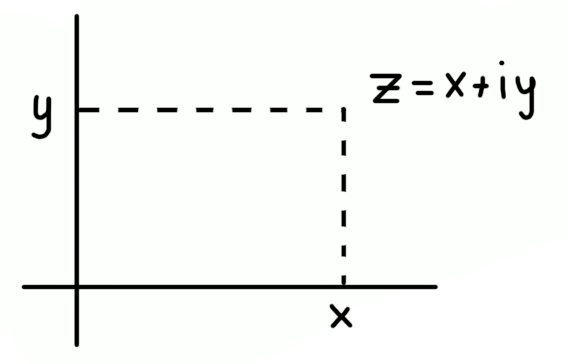
\includegraphics[width=0.9\linewidth]{kompl/1kompl.png}
\end{wrapfigure}

 К.ч. $z$ и $-z$ симметричны относительно начала координат. Числа $z$ $\overline{z}$ ассиметричны относительно действительной оси.
 
 К.ч. можно трактовать также, как вектор с началом в точке $О$ и концом в $Z$, т.е. радиус вектор точки ($x$,$y$). Это точка биекция.
 
 Число $z_1+z_2$ - вектор равный сумме векторов $z_1$ и $z_2$
 
 $z_1-z_2$ - вектор равный разности
 \par\bigskip
 Очевидно, что число $|z_1-z_2|$ - представляет собой расстояние между точками $z_1$ и $z_2$
 
 Отметим, что из геометрической интерпретации к.ч. вытекают неравенства:
 $$||z_1|-|z_2|| \leqslant |z_1-z_2| \leqslant |z_1|+|z_2|$$
$$\left|\sum\limits_{k=1}^n z_k\right| \leqslant \sum\limits_{k=1}^n |z_k|$$

 \par\bigskip\textbf{Пример 1} : Множество точек комплексной плоскости удовлетворяющих соотношению $|z-z_0|=R$ есть окружность раудиуса $R$ с центром в точке $|z_0|$. Обозначаем $S(z_0; R)$
    \par\bigskip
 \textbf{Пример 2} : {$z| z \in \mathbb{C}, |z-z_0| < R$} открытый круг радиуса R с центром в точке $Z_0$: $B(z_0; R)$
    \par\bigskip
 \quad Замкнутый круг $\overline{B}(z_0; R) = \left\{z| z \in \mathbb{C}, |z-z_0|\leqslant R  \right\} $
   \par\bigskip
 \quad Кольцо $B(z_0; 2; R)$ = $\left\{z| z \in \mathbb{C}, 2 < |z-z_0| < R  \right\}$
 \par\bigskip



  \subsection{Тригонометрическая и показательная формы к.ч.}  

Точки на плоскости можно задать не только через декартовы, но и через полярные координаты $z, \phi$, где $z=|z|$ - модуль расстояния от 0 до $z$, а $\phi$ - угол между положительным направлением действительной оси и вектором $z$ (3 искомых угла по общему правилу) этот угол называют аргументом комплексного числа $z:\; (z\neq 0)$ и обозначают $\phi=Arg\, z$. \par\bigskipДля\quad $z=0\quad Arg\, z$ не вводится.
 \par\bigskip
 Значение аргумента определяется с точностью до целого числа  (кратного 2n)
 \par\bigskip
 Чтобы устранить эту неодназначность, условились что:
 $$\varphi_0 \leqslant \varphi \leqslant \varphi_0+2\pi$$
 
 т.е. выбирают аргумент на промежутке длинны $2\pi$. Выбор $\phi_0$ - произволен. Чаще всего $-\pi < \phi \leqslant \pi$ либо $0 \leqslant \phi < 2\pi$. Выбранный таким образом аргумент называют \textbf{главным значением аргумента} и обозначают его $Arg\, z$
 \par\bigskip
 Таким образом $Arg\, z = arg\, z + 2\pi k$, $k\in \mathbb{Z}$ из связи декартовых и  вытекает, что:
 $$x=\rho\, cos\varphi,\quad y=\rho\, sin\varphi,\quad \text{поэтому}\   z=x+iy=\rho (cos\varphi+isin\varphi)$$
 
 Эта форма к.ч. называется \textbf{тригонометрической формой}.
 \par\bigskip
 В другом виде
 
 $$z=|z|(cos Arg\, z+iArg\, z)$$
 \par\bigskip
 Аргумент $\varphi = Arg\, z$ удовлетворяет соотношению 
 
 $$tg\varphi=\frac{y}{x}$$
 
 но не все значения $\varphi$ являются аргументом. А именно:
 
\begin{equation*}
Arg z= 
 \begin{cases}
   arctg \frac{y}{x}, x>0\\
   $\pi + arctg\frac{y}{x}, x<0, y\geqslant0$ \quad\quad   если $-\pi<\varphi\leqslant\pi$ \\
   $\pi+arctg\frac{y}{x}, x<0, y\geqslant0$\\
 \end{cases}
\end{equation*}

 На практике эта формула не используется, а $arg\,z$ выбирают с учётом знакопостоянства $z$ на плоскости.
 \par\bigskip
 \textbf{Пример:} найти модуль и аргумент числа $z=1-i$ и записать число в тригонометрической форме.
 
 $|z|=\sqrt{1+1}=\sqrt{2}$;\quad $arg z=arctg(-1)= 
 \begin{cases}
   \frac{-\pi}{4}, \quad -\pi<\varphi\leqslant\pi \\
   \frac{7\pi}{4}, \quad 0\leqslant\varphi<2\pi
 \end{cases}$

 $1-i=\sqrt{2}(cos(\frac{-\pi}{4})+isin(\frac{-\pi}{4}))$

\par\bigskip
 Вы уже знакомы с формулами Эйлера

 $$e^{i\varphi}=cos\varphi+isin\varphi$$
\par\bigskip
 Поэтому, очевидно, что к.ч. $z$ может быть представимо в виде (экспотенциальная формула к.ч.) 
 
 $$z=\rho\,e^{i\varphi}=|z|e^{iarg z}=|z|e^{iArg z}$$
 
 z -- модуль, $\varphi$ -- аргумент
 \par\bigskip
 Отметим:\quad $e^{2\pi i}=1,\quad e^{\pi i}=-1,\quad e^{\frac{\pi i}{2}}=i, e^{\frac{-\pi i}{2}}=-i$
 
 $|e^{i\varphi}|=1\quad \forall \varphi \in \mathbb{R}$
 
 \parТригонометрическая и показательная форма комплексного числа очень удобны при умножении и делении:
 
 $$z_1z_2=|z_1| e^{i\varphi_1}|z_2|e^{i\varphi_2}=|z_1||z_2|e^{i(\varphi_1+\varphi_2)}$$
 
 $$\frac{z_1}{z_2}=\frac{z_1e^{i\varphi_1}}{z_2e^{i\varphi_2}}=\frac{z_1}{z_2}e^{i(\varphi_1-\varphi_2)}$$
 \par\bigskip
 Отсюда вытекают равенства:
 $$arg z_1z_2=arg z_1+arg z_2$$
 $$arg\frac{z_1}{z_2}=arg z_1-arg z_2$$

 с точностью до $2\pi$
 \par\bigskip
 \textbf{Формула Муавра}

$$z^n=(ze^{i\varphi})^n=z^ne^{in\varphi}$$

 или

$$(cos \varphi+isin \varphi)^n=cos n\varphi+isin n\varphi$$

\par\bigskip
 Тригонометрическая и показательная формулы позволяют легко вычислить корни из к.ч.
 
 \par\bigskip $z^n=c,\ c\in \mathbb{C},\ c\neq 0,\ n\in \mathbb{N} $
 \par\bigskip
 Поставим задачу найти все комплексные корни $z$ этого уравнения. 
 \par\bigskip
 Пусть $c=z_0e^{i\varphi_0},\ z=ze^{i\varphi}$

 Тогда $z^n=z_0,\ n\varphi=\varphi_0+2k\pi$
 
 Поэтому $z=\sqrt[n]{z_0};\ \varphi_k=\frac{\varphi+2k\pi}{n} \quad \quad k=0,1,...,n-1$

 Значения $k$ можно брать из всего $\mathbb{Z}$, но всего n различных.

 На комплексной плоскости эти значения находятся в вершинах правильного n-угольника, вписанного в окружность радиуса $\sqrt[n]{z_0}$
 \par\bigskip
 \textbf{Пример.}\quad $\sqrt[n]{1}=\left\{1,-1,i,-i\right\}$
 
 
 
 \subsection{Последовательности комплексных чисел}  
 
 
 Рассмотрим последовательность ($z_n$) к.ч.
 \par\bigskip
 Число $c\in\mathbb{C}$ называют \textbf{пределом последовательности} ($z_n$), если 
 
 $$\forall\varepsilon>0 \quad \exists\nu(\varepsilon)>0 \quad\forall n\geqslant\nu(\varepsilon) \Rightarrow |z_n-c|\leqslant\varepsilon$$
 
 или 
 
 $$\forall V_\varepsilon(c) \quad \exists\nu_\varepsilon>0 \quad \forall n\geqslant\nu_\varepsilon \Rightarrow z_n\in V_\varepsilon(c)$$
 
 или
 
 \begin{center}
     $\lim_{n\to \infty} |z_n - c|=0$\ \text{-- действительная последовательность}
 \end{center}

Обозначения стандартные:\quad $\lim_{n\to \infty} z_n=c,\quad \lim z_n=c,\quad z_n\rightarrow c,\quad n\rightarrow\infty$
\par\bigskip
Геометрический смысл
\par
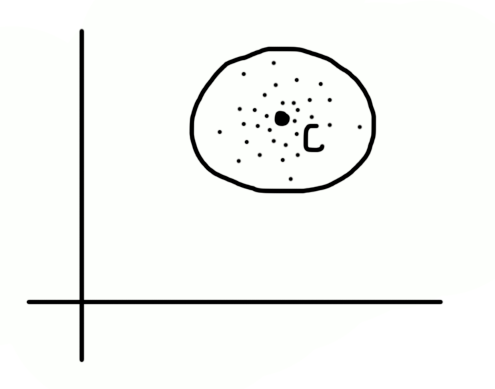
\includegraphics[width=0.3\linewidth]{kompl/2kompl.png}
  
\par\bigskip
Последовательность имеющую классический предел назовём \textbf{сходящейся}
\par\bigskip
Каждой последовательности к.ч. ($z_n$) соответствуют две последовательности действительных чисел \\($x_n$) и ($y_n$), где $z_n=x_n+iy_n$

\par\bigskip
\textbf{Теорема:}\quad \textit{Существование предела $lim\, z_n=c$ равносильно существованию двух пределов $lim x_n$ и $lim y_n$, при этом $lim\, z_n=lim\, x_n+ilim\, y_n$}
\bigskip

\begin{wrapfigure}[6]{r}{0.2\linewidth} 
    \vspace{-1ex}
    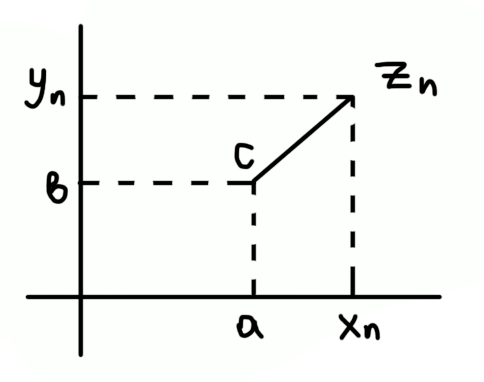
\includegraphics[width=0.9\linewidth]{kompl/3kompl.png}
\end{wrapfigure}

$\blacklozenge$\hspace{2 mm} Пусть $c=a+ib$
 
 $\Rightarrow \quad lim\, z_n=c$ 
 \par\bigskip
 $|x_n-a|\leqslant|z_n-c|\leqslant\varepsilon$ (катет меньше или равен гипотенузе)
 
 $|y_n-b|\leqslant|z_n-c|\leqslant\varepsilon$
 \par\bigskip
  $\Rightarrow$ \quad $|z_n-c|=|(x_n-a)+i(y_n-b)|\leqslant|x_n-a|+|y_n-b|\leqslant2\varepsilon$
  
  (Сторона треугольника меньши суммы двух других ) \quad $\blacksquare$
  \par\bigskip
  Из определения предела и доказанной теоремы вытекают общие свойства:

  \begin{enumerate}
\item[1)] Критерий Коши сходимости
\item[2)] Принцип Вебера
\item[3)] Арифметика пределов
\item[4)] $lim z_n=c \quad \Rightarrow \quad lim|z_n|=|c| (||z_n|-|c||\leqslant|z_n-c|)$
\item[5)] $lim z_n=z_0,\ lim\varphi_n=\varphi_0\quad \Rightarrow \quad limz_n=z_0e^{i\varphi_0}$
\end{enumerate}

 
 \subsection{Расширенная комплексная плоскость}  
 
 Плоскость комплексных чисел называется \textbf{сходящейся к бесконечности}, если $lim z_n=+\infty$. \parЗапись:\quad $lim\, z_n=\infty$
 
 Другими словами:\quad $\forall\varepsilon>0, \exists\nu_\varepsilon, \forall n\geqslant\nu_\varepsilon\quad\Rightarrow\quad|z_n|\geqslant\varepsilon$
 
 Геометрически это означает, что $z_n$ лежит вне круга радиуса $\varepsilon$. Это множество называют \textbf{окрестностью бесконечности} и обозначать будем $B(0;\ \varepsilon;\ +\infty)$.
 
 Следовательно, точка $z=\infty$ является пределом последовательности $(z_n)$, если в $\forall$ окрестности точки $z=\infty$ содержаться все члены этой плоскости, за исключением конечного их числа.
 
 Таким образом, символу $z=\infty$ ставится в соответствие символическая бесконечно удалённая точка.
 
 \par\bigskip
 \textbf{Определение:}\quad комплексную плоскость, наполненную бесконечно удалённой точкой называют \textbf{расширенной комплексной плоскостью}.
 \par\bigskip
 \newpage
 Наглядное представление расширенной комплексной плоскости даёт следующая геометрическая интерпретация:
 \begin{wrapfigure}[9]{l}{0.35\linewidth} 
    \vspace{-2ex}
    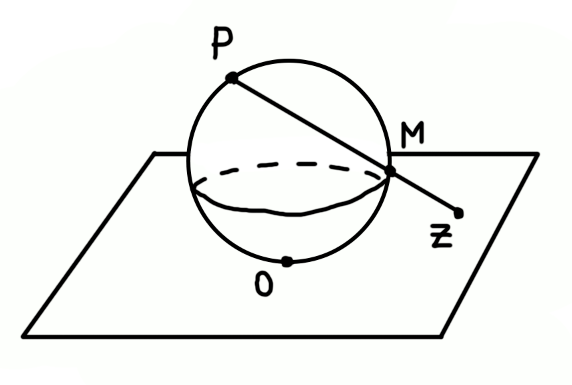
\includegraphics[width=0.9\linewidth]{kompl/4kompl.png}
\end{wrapfigure}
 
 Рассмотрим сферу S, касающуюся комплексной плоскости в т. $O$. Обозначим через $P$ точку сферы, диаметрально противоположную точке $O$. Каждой точке $z$ комплексной плоскости поставим в соответствие точку $M$, которая является точкой пересечения сферы с отрезком, соединяющим $Z$ и $P$
 
 Ясно, что при этом последовательности $Z_n$, сходящейся к $\infty$, соответствует последовательность точек сферы $S$, сходящаяся к $P$. Поэтому точке $P$ поставим в соответствие точку $z=\infty$.
  
 
 Такое соответствие между точками комплексной плоскости и точками сферы $S$ является взаимно однозначными. Оно называется \textbf{стереографической проекцией}, а сфера $S$ называется \textbf{сферой Римана}.
 \par\bigskip
 Комплексные числа (включая $z=\infty$) можно изображать точками сферы Римана. При этом, сходящиеся последовательности к.ч. изображаются на сфере Римана сходящимися последовательностями. 
 
 При стереографической проекции окружности переходят в окружности, угол между пересекающимися кривыми на плоскости равен углу между образами этих кривых на сфере Римана.
 
 В такой интерпритации $z=\infty$ выступает как обычная точка, однако  не будем рассматривать. 
 
 \par\bigskip
 Иногда будем употреблять обозначения:
  \begin{enumerate}
\item ]$-\infty,\ +\infty$[ -- действительная ось 
\item ]$-i\infty,\ +i\infty$[ -- мнимая ось
\item ]$\alpha-i\infty,\ \alpha+i\infty$[ -- $Re\,z=\alpha$
\item ]$\beta i-\infty,\ \beta i+\infty$[ -- $Im\, z=\infty$
\end{enumerate}

\textbf{Утверждение.}\quad Расширенная комплексная плоскость - есть замкнутое множество (даже больше компакт).

Прямая в расширенной комплексной плоскости замкнута.




\section{Комплексные функции действительного аргумента}
\par\bigskip
Пусть $z = \sigma (t)$ определена  на отрезке $[\alpha, \beta] \subset \mathbb {R} $ и принимает комплексные значения, т.е $\sigma: [\alpha, \beta] \to \mathbb{C}$. Такую функцию можно представить в виде:
\begin {equation}
\sigma (t) = \xi(t) + i \eta (t)
\end {equation}
\\где $\xi (t)$ = Re $\sigma (t)$; $\eta(t)$ = Im $ \sigma (t)$ --- действительные функции.

\par\bigskip
\textit{Многие свойства действительных функций переносятся на комплексно-значные функции:}
\par\bigskip
Предел функции $\sigma (t)  = \xi(t) + i\eta(t)$ определяем формулой $\lim\limits_{t \to t_0} \sigma (t) = \lim\limits_{t \to t_0} \xi (t) + i\lim\limits_{t \to t_0} \eta (t).$
\par\bigskip Таким образом предел $\sigma(t)$ существует, если существуют пределы функций $\xi (t), \eta (t)$.
Это определение эквивалентно такому  утверждению:
\begin {equation}
\lim\limits_{t \to t_0} \sigma(t) = a \iff \ \forall \varepsilon  > 0 \ \exists \  \delta_\varepsilon > 0 \ \forall \  t, 0 < |t - t_0| \leq \delta_\varepsilon \implies |\sigma (t) - a| \leq \varepsilon
\end{equation}

Функцию $\sigma (t)$ назовем \textbf{непрерывной в точке (на отрезке)}, если в этой точке (на этом отрезке) непрервыны функции $\xi (t)$ и $ \eta(t)$.
\par\bigskip Нетрудно увидеть, что это определенние равносильно следующему утверждению:
\par $\sigma(t)$\text{ - непрерывна в точке }  $t_0\ \iff \ \lim\limits_{t \to t_0} \sigma (t) = \sigma(t_0)$
\par
$\forall \ \varepsilon > 0 \ \exists \ \delta_\varepsilon > 0 \ \forall \ t, |t - t_0| \leq \ \delta_\varepsilon \implies |\sigma(t) - \sigma(t_0)| \leq \varepsilon$
\par\bigskip
Сумма, разность, произведение, частное (со знаменателем, отличным от нуля) непрерывных функций, есть функция непрерывная.

\par\bigskip
Если $\sigma(t)$ непрерывна на отрезке, то она \textbf{ограничена} на этом отрезке, т.е. $\exists$ M такое, что $|\sigma (t)| \leq M \ \forall t$

Производная вычисляется по формуле (имеют место основные правила вычисления производных)
\begin{equation}
 \sigma'(t) = \lim\limits_{\Delta t \to 0} \frac{\sigma(\Delta + \Delta t) - \sigma (t)} {\Delta t}
\end{equation}
\par Однако не все теоремы действительного анализа  переносятся на комплексно-значные функции: например не имеют места т. Ролля и ... 
\par\bigskip
\textbf{Пример.} \quad $\sigma(t) = e^{it}$ дифференцируема на $ [0, 2\pi]$
\par $\sigma' = ie^{it}$, но $|\sigma '(t)| = |ie^{it}| = 1$ \ для $t \in [0, 2\pi]$ \ хотя $\sigma (0) = \sigma (2\pi) = 1$
\par\bigskip
Определение интеграла: $\int\limits_\alpha^\beta \sigma(t)dt = \int\limits_\alpha^\beta \xi(t)dt + i\int\limits_\alpha^\beta \eta(t)dt $  
\par
Это определение экивалентно определению с помощью интегральных сумм.
\par\bigskip
\textbf{Имеют место обычные формулы:}
\begin{enumerate} 
  \item  $\int\limits_\alpha^\beta (a_1\sigma_1(t) + a_2\sigma_2(t))dt =a_1\int\limits_\alpha^\beta \sigma_1(t)dt$ + $a_2\int\limits_\alpha^\beta \sigma_2(t)dt$
  \item  $\int\limits_\alpha^\beta \sigma(t)dt = - \int\limits_\beta^\alpha \sigma(t)dt $
  \item Аддитивность: $\int\limits_\alpha^\gamma \sigma(t)dt +   \int\limits_\gamma^\beta \sigma(t)dt = \int\limits_\alpha^\beta \sigma(t)dt$
  \item Формула Ньютона-Лейбница
  \item $|\int\limits_\alpha^\beta \sigma(t)dt| \leq \int\limits_\alpha^\beta |\sigma(t)|dt$
\end{enumerate}
Но не верна теорема о среднем.
\\На комплексно-значную функцию можно смотреть как на вектор-функцию.
\par\bigskip
\section{ Кривые в $\mathbb{C}$}
На кривую $l$ в комплексной плоскости можно смотреть как на кривую в $\mathbb{R}^2$.
\par
Пусть $\sigma: |\alpha, \beta| \to \mathbb{R}^2 $, представление кривой $l$.
\parТогда $\vec\eta = \sigma(t), t \in |\alpha, \beta|$ - её векторно -приближенное уравнение, которое можно записать так:
\begin{equation*}
 \begin{cases}
   x = \xi(t)
\\
	y = \eta(t)
 \end{cases}
t \in |\alpha, \beta|, \text {где $\xi(t)$ и $\eta(t)$ - координатные функции $\sigma$}
\end{equation*}
\\ Но мы знаем, что между множеством комплексных чисел и множеством точек плоскости устанавливаются взаимно-однозначное соответствие $z = x + iy$.
\\Поэтому $z = x(t) + iy(t) = \xi(t) + i\eta(t) = :: \sigma(t), t \in [\alpha, \beta], \sigma$ -  комплексно-значная функция.
\par\bigskip
Уравнение $z=\sigma(t), t \in |\alpha, \beta|$ называют \textbf{параметрическим уравнением кривой $l$ на комплексной плоскости}.
\\Незамкнутую кривую $l$ всегда будем считать ориентированной в направлении возрастания параметра t, и это направление будем называть \textbf{положительным}, а противоположное ему \textbf{отрицательным}. 
\\ $\sigma(\alpha)$ - начало кривой, $\sigma(\beta)$ - конец кривой.
\\ \\ \textbf{Пример: } 
\begin{enumerate}
    \item $z = \cos t, \pi < t \leq 2\pi$
    \begin {equation*}
	\begin{cases}
	x =\cos t \\
	y = 0
	\end{cases}
	\ \ \ \ 
\begin{tikzpicture}
\draw[ultra thick, black] (-1,0) -- node[shift = {(-1, -0.4)}]{$-1$} (1, 0) -- node[shift = {(0, -0.4)}]{$1$} (1,0);
\end{tikzpicture}
\end{equation*}
\item $z = e^{it}, 0 \leq t < 2\pi$ - окружность,  $|z|=1$ \ ориентированная так, что направление движения против часовой стрелки.
\item $z = z_0 + e^{it}, 0 \leq t < 2\pi, |z - z_0| = 1$
\item $z = z_0 + Re^{it}, 0\leq t < 2\pi, |z- z_0 = R|$
\end{enumerate}

\par\bigskip
Для кривой в $\mathbb{C}$ сохраняются все определения для плоских кривых.
\\Например, \textbf{кривая простая}, если она не имеет самопересечений, т.е $t_1 \neq t_2 \implies \sigma(t_1) \neq \sigma(t_2)$. Если начало и конец совпадают, то это не самопересечение.
\par\bigskip
\textbf{Спрямляемая кривая} - имеющая длину $l = \int\limits_\alpha^\beta \sqrt{\xi'(t)^2 + \eta'(t)^2}dt = \int\limits_\alpha^\beta |\sigma'(t)|dt$
\par\bigskip
\textbf{Гладкая кривая}
\\$\sigma(t)$ -- непрерывно-дифференцируема и $\sigma$'(t) $\neq$ 0, t $\in$ |$\alpha, \beta$|, $\sigma'(t)$ -- вектор касательной.
\par\bigskip

\section{Области в $\mathbb{C}$}
Все определния сохраняются как и в $\mathbb{R}^2$.
\par \textbf{Область} --- открытое связное множество.
\par \textbf{Компакт} --- замкнутое ограниченное множествo.
\par\bigskip
Дальше рассматриваем область, границы которой состоят из конечного числа кусочно-гладких кривых и изолированных точек.
\\Ориентация границы $\partial D$ области $D$ считаем \textbf{положительной}, если при движении по границе $\partial D$ область останется слева.
\par\bigskip
\textbf{Примеры:}
\begin{enumerate}
    \item $B(z_0, 0, R)$ - круг с выколотой точкой, проколотая окрестность точки $z_0$, центрированная окрестность $0 < |z-z_0|<R$ 
\item круг с разрезом 
\item кольцо $B(z_0;z;R)$
\item Расширенная комплексная плоскость --- односвязна
\item Расширенная комплексная плоскость с выброшенной точкой --- односвязна
\end{enumerate}


\par\bigskip
\section{Функции комплексной переменной}
\par\bigskip
Пусть $D \subset \mathbb{C}$ (множество комплексных элементов), и каждому $z \in D$ поставленно в соответствие одно или несколько комплексных чисел $w$. Тогда говорят, что на $D$ задана функция. 
\par\bigskip
$f: D \to \mathbb{C}, D \subset \mathbb{C}$ или $f: z \mapsto w, w = f(z), \ x + iy \longmapsto u + iv$
\par\bigskip Комплексному числу ставится в соответствие комплексное число.
\par $w(z) = u(x,y) + iv(x,y)$,\quad где $u(x,y) = Re\,w(z), v(x,y) = Im\,w(z)$ --- действительные функции. 
\par\bigskip Таким образом комплексную функцию можно рассматривать как пару действительных функций действительных аргументов $x, y$. 
\par\bigskip
 Многие свойства ФКП можно получить исходя из такой связи.
\\Если каждому $z$ отвечает одно значение $w$, то функцию $w = f(z)$ называют \textbf{однозначной}. Если же некоторым $z$ соответствует более одного $w$, то $f$ называют \textbf{многозначной}.
\par\bigskip
Если $f:D \to G$, то можно поставить вопрос об обратной функции $f^{-1}: G \to D, \\ z = f^{-1}(w).$
\par\bigskip
Если обратная функция неоднозначна, то функцию $f$ называют \textbf{неодноместной}. Если $f^{-1}$ --- однозначна, то $f$ --- \textbf{одноместна.}
\\Другими словами, $f$ --- \textbf{одноместна} на множестве $D$, если $\forall z_1, z_2 \in D$ равенство \\$f(z_1) = f(z_2)$ имеет место тогда и только тогда, когда $z_1 = z_2$. 
\par\bigskip
Геометрически  будем интерпретировать следующим образом: график функции комплексного переменного изобразился бы некоторой  поверхностью в трёхмерном пространтве $x, y, u, v$. Однако неявно это трудно представить, поэтому обычно поступают так: интерпретируют геометрически $f$ как отображение множеств на разных плоскостях. Так хорошо, но трудно рисовать и плохо видно.
\\ 
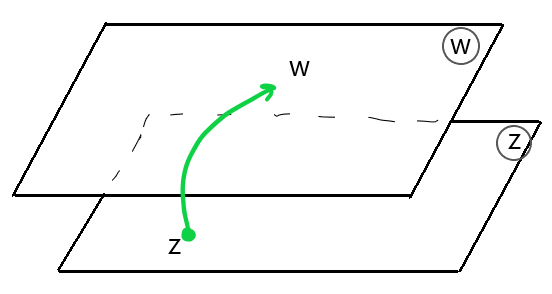
\includegraphics[scale = 0.75]{im1} \ поэтому будем рисовать иначе
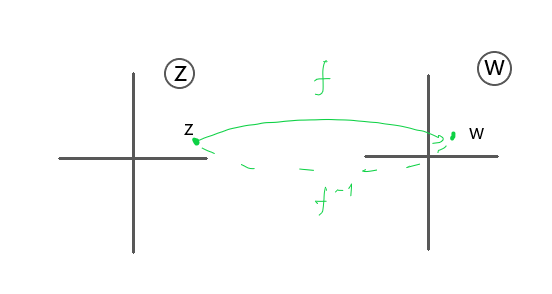
\includegraphics[scale = 0.5]{im2}
\\ Иногда плоскости $z$ и $w$ совмещают (как полярные и декартовы координаты).
\\ 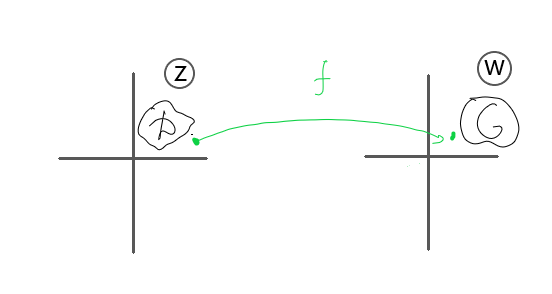
\includegraphics[scale = 0.5]{im3}
\\ $w = f(z)$, то $w$ называют \textbf{образом точки $z$ при отображении $f$}, а $z$ \textbf{прообразом}. Аналогично $G$ --- \textbf{образ}, $D$ --- \textbf{прообраз}. 
\par\bigskip Композиция: $f \circ g$:
\\ 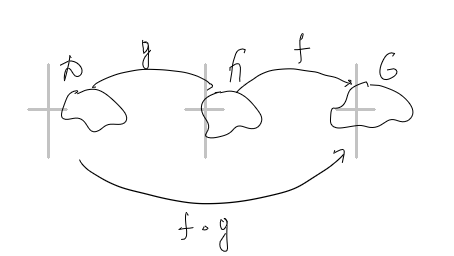
\includegraphics[scale = 0.75]{im4}
\par\bigskip
\textbf{Примеры:}
\\ $w = arg\ z$ - однозначная, обратная неоднозначная.
\\ $w = Arg\ z$ - неоднозначна, неодноместна.
\\ $w = z^2$ - однозначна, неодноместна.
\\ $w = \sqrt{z}$ - неоднозначна.
\\ $w = \bar z$ - однозначна, одноместна.
\par\bigskip


\section{Предел функции комплексной переменной}
Пусть точка $z_0$ является предельной точкой множества $D$. Число $A$ называется \textbf{пределом} функции $f$ при $z \to z_0$, если:
\begin{equation}
	\forall \  V(A) \  \exists \ \dot U (z_0) \ \ \ \ \ \ \ \ \ \ f(\dot U (z_0)) \subset V(A)
\end{equation}
\\ Другими словами:$A$ --- предел $f$, если
\begin{equation}
	\forall \ \varepsilon \ > 0 \ \exists \ \ \delta_\varepsilon > 0 \ \ \ \ \forall z \in B(z_0, 0, \delta_\varepsilon) \cap D \implies f(z) \in B(A; E)
\end{equation}
или
\begin{equation}
A = \lim\limits_{z \to z_0} f(z), \text{если} \ \forall \ \varepsilon \ > 0 \ \exists \ \ \delta_\varepsilon > 0 \ \ \forall \ z \in D,\ \ 0\ <|z - z_0| \leq \ \delta_\varepsilon \implies |f(z) - A|\leq \varepsilon
\end{equation}
или
\begin{multline}
	\\
	A = \lim\limits_{z \to z_0} f(z), \text{если} \lim\limits_{z \to z_0}|f(z) - A| = 0\\
	\exists \lim\limits_{z \to z_0} f(z) = A \iff \exists \  \text{два предела} \lim\limits_{x \to x_0,\  y \to y_0} u(x,y) и \lim\limits_{x \to x_0,\  y \to y_0} v(x,y)
	\\
	\text{причём} \lim\limits_{z \to z_0}f(z) = \lim\limits_{x\to x_0, y \to y_0} u(x,y) + i \lim\limits_{x \to x_0, y \to y_0} v(x,y)
\end{multline}
\par\bigskip
Имеет место \textbf{критерий Гейне}:
\\Для того чтобы $f(z) \rightarrow A$ при $z \rightarrow z_0 \iff \ \forall (z_n), z_n \in D, \ z_n \neq z_0, z_n \to z_0 \implies f(z_n)  \to A$, при $n \to \infty$.
\par\bigskip
Из изложенных фактов вытекает, что на предел ФКП можно перенести простейшие предложения, относящиеся к пределам функций двух действительных переменных (суммы, произведения, частного и т.д.).
\\В теории ФКП используют следствие Ландау, о, О, n, которые имеют тот же смысл, что и в действительном анализе.

\par\bigskip
\section{Непрерывность функций коплексной переменной}
\par Пусть $z_0 \in D$ и $f:D \to \mathbb{C}$
\par $f$ называют \textbf{непрерывной} в точке $z_0$, есл $\lim\limits_{z\to z_0}f(z) = f(z_0)$.
\par Исходя из определения предела и непрерывности, заключаем, что можно привести множество равносильных формулировок:
\begin{enumerate}
\item $f$ непрерывна в точке $z_0$, если \\ $\forall \varepsilon > 0 \ \ \ \exists \ \delta(\varepsilon) > 0 \ \  \forall z,\ \ |z - z_0|\leq \delta(\varepsilon) \implies |f(z) - f(z_0)| \leq \varepsilon $
\\ Непрерывность $f$ в точке $z_0$ равносильна непрерывности $u(x,y)$ и $v(x,y)$ в точке $(x_0, y_0)$
\\ Это позволяет перенести на ФКП многие свойства Ф2П. Например аримфметики непрерывных функций. 
\\ Функцию $f$ назовем \textbf{непрерывной}  на множестве $D$, если она непрерывная в каждой точке этого множества. 
\\Аналогично, как и в действительном анализе вводятся понятия о \textbf{равномерной непрерывности}.
\end{enumerate}
\par\bigskip
\textbf{Примеры:}
\begin{enumerate}
    \item z, Rez, Imz, $\bar z$, |z| - непрерывны на $\mathbb{C}$.
    \item P(z) непрерывна на $\mathbb{C}$.
    \item $\frac{P(z)}{Q(z)}$ - непрерывны там, где заданы и $Q(z) \neq 0$.
\end{enumerate}

\par\bigskip
Отметим также и \textbf{свойства}:
\begin{enumerate}
    \item $f \in C(D)$ и $f$ - биекция $D$ на $G$, то $D$ - область $\implies$ $G$ - область и $f^{-1} \in C(G)$ 
\item Если $f \in C(\bar D) \bar D$ $f$ - ограничена в $D$, т.е $\exists M > 0$, что $|f(z)|\leq M \ \forall z \in D$, причём $|f(z)|$ достигнет в $\bar D$ своих наибольшего и наименьшего значений(следствие т.Вейерштрасса для Ф2П и $|f| = \sqrt{n^2 + v^2}$). Имеет место аналог т. Кантора.
\end{enumerate}

\par\bigskip
Аналогично определяется непрерывность $f$ в бесконечно удалённой точке $z_0 = \infty$:\\ $f$ -- непрерывна в $z_0 = \infty$ $\lim\limits_{z \to z_0},если f(Z) = f(\infty)$






\section{Элементарные функции комплексного переменного}

\subsection{Линейная функция} 
\hspace{1 mm}

$w = f(z) = az$,\quad a $\in \mathbb{C} $ --- непрерывна на $ \mathbb{C}$.  

\par\bigskipЕсли $ a \neq 0,$ то она биективна и для нее существует обратная функция $z = \frac{1}{a}w$ и имеет обозначение $w = f^{-1}(z) = \frac{1}{a}z$ - тоже линейная. Поскольку обратная однозначная, то исходная однолистна.

\bigskip{$w = f(z) = az = \left\lvert a \right\rvert \left\lvert z \right\rvert e^{i(\theta +\varphi  )}$,  
где $a = \left\lvert a \right\rvert e^{i\theta }, z = \left\lvert z \right\rvert e^{i\varphi  }\Rightarrow \left\lvert w\right\rvert = \left\lvert a\right\rvert \left\lvert z\right\rvert$}

\par $arg$\hspace{1 mm}$ w $ = $ arg$\hspace{1 mm}$ a + arg$\hspace{1 mm}$ z$
\bigskip

Из этих двух соотношений следует способ построения образа при линейном отображении:

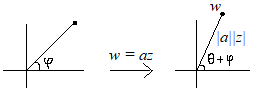
\includegraphics{5-6/1io.png}

Таким образом функция $w = f(z) = az$ осуществляет растяжение в $\left\lvert a \right\rvert$ раз и поворот на угол $\theta = arg$\hspace{0.2 mm}$z$.

Функцию $w = az + b$ тоже называют линейной функцией. Образ, получившийся при отображении $w = az $ ещё отличается на вектор b.

\par\bigskip\textbf{Пример.} \quad Найти образ $\left\lvert z\right\rvert < 1$ при отображении $w = 2iz + 1 + i$

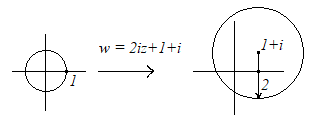
\includegraphics{5-6/2io.png}

\subsection{Степенная функция}
\subsection*{1)$\hspace{3 mm} w = f(z) = \frac{1}{z} $} 

\par{Непрерывная для $z\neq 0$, биективная, обратимая.} 

$f^{-1} = \frac{1}{z},\ w = \rho e^{i\theta },\ z = re^{i\varphi }$

Тогда $\rho\, e^{i\theta } = \frac{1}{r\,e^{i\varphi }} = \frac{1}{r} e^{-i\varphi }\quad \Rightarrow \quad \rho = \frac{1}{r},\ \theta = -\varphi   $.
 \ То есть, $\left\lvert w\right\rvert = \frac{1}{\left\lvert z\right\rvert },\  arg\hspace{1 mm}w = arg\hspace{1 mm}z.  $

Геометрическая картинка:

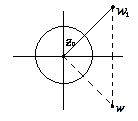
\includegraphics{5-6/3io.png}
\par
Точки внутри круга отображются в точки вне круга и наоборот (инверсия относительно единичной окружности, затем зеркальное отображение относительно действительной оси).
Внутренность круга отображается во внешность и наоборот. Лучи в лучи. Окружности в окружности.

\subsection*{2)$\hspace{3 mm} w = z^n, n\in \mathbb{N} $}

Функция непрерывная. Определена в $\mathbb{C} $. Однозначна, но не однолистна. 

$z = re^{i\varphi }, w = \rho e^{i\theta }$

$\rho e^{i\theta } = r^ne^{in\varphi }\Rightarrow \rho = r^n$, т.е. $\left\lvert w \right\rvert = \left\lvert z \right\rvert^n  $, $arg\hspace{1 mm}w = n\hspace{1 mm} arg\hspace{1 mm}z$ (с точностью до $2k\pi $).

Функция необратима на всей плоскости, т. $z, z = \sqrt[n]{w} $, и для каждого w получаем n значений z, т.е. функция $w = z^n$ не инъективна или, по-другому, неоднолистная во всей плоскости. 

Найдем множество однолистности 

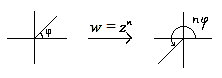
\includegraphics{5-6/4io.png}

То есть луч поворачивается на угол $n\varphi $. Сектор с радиусом\textbf{(?)} $\frac{2\pi }{n} $ и нулём в центре переходит в плоскость с разрезом. 

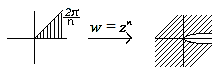
\includegraphics{5-6/5io.png}

Каждый из секторов ...(разрез???)... $\frac{2\pi }{n} $ отображается на всю плоскость.

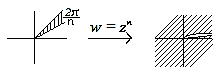
\includegraphics{5-6/6io.png}

\subsection*{3$)\hspace{3 mm} w = \sqrt[n]{z} , n\in \mathbb{N} $}

Это функция обратная степенной. Приходится выбирать ветки. Это делается исходя из формулы:

\quad{$\sqrt[n]{z} = \sqrt[n]{z} e^{i\frac{\varphi +2k\pi }{n}  } $ \quad и достигается выбором k.}

Т.е. функция $w = \sqrt[n]{z}$ многозначна, но можно выбрать k однозначных ветвей. Действие обратное степенной. (Плоскость с разрезом на ... $\frac{2\pi }{n}. $)

\subsection{Экспонента}
\begin{center}
    \textbf{$w = e^z$}
\end{center}

Может быть определена формулой 

\begin{center}
    $ e^z = e^{x+iy} = e^xe^{iy} = e^x(\cos y + i\sin y)$
    \par Re $e^z = e^x\cos y$
    \par Im $z = e^x\sin y$
\end{center} 



\par\bigskipОтсюда вытекают следующие свойства:
\par\bigskip
\begin{enumerate} 
  \item $e^{z_1}e^{z_2}=e^{z_1+z_2},$\quad$\forall z_1,z_2\in\mathbb{C}$
    
  \item $e^{z+2k\pi i}=e^z,$\quad$\forall z\in \mathbb{C}$
  \par т.е. функция $e^z$ --- периодическая с периодом $2k\pi$$i$ 
  \par Поэтому функция $e^z$ неоднолистна (хотя и однозначна). В точках $z+$$2k\pi$$i$ она принимает одинаковые значения.
  
  \item $e^z$ непрерывна во всей комплексной плоскости.
  
  \item $|e^z|=e^x$,$\quad$ $Arge^x=y+$$2k\pi$
\end{enumerate}

\par\bigskipИз этих соотношений вытекает геометрический характер отображения:

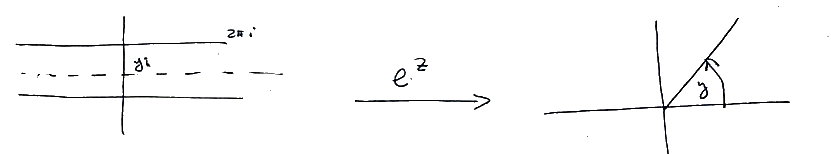
\includegraphics[width=15cm, height=3cm]{exponenta 7/exp.png}

$-\infty<x<+\infty$\quad$\Rightarrow$$\quad$$0<e^x<+\infty$,$\qquad$ $\qquad$$|w|\in$ $\left]0,+\infty\right[$,$\quad$$\arg e^z=y$

\par\bigskip

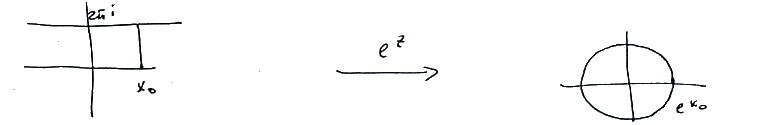
\includegraphics[width=16cm, height=3cm]{exponenta 7/exp2.png}

 $z=x_0+iy$,$\quad$$0<y<2\pi$,$\qquad$ $\qquad$ $|w|=e^{x_0}$,$\quad$$0<\arg w<2\pi$
\par\bigskip
Кроме того,

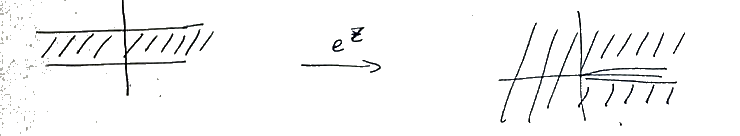
\includegraphics[width=14cm, height=3cm]{exponenta 7/exp3.png}

\subsection{Логарифм}
\begin{center}
    \par\bigskip {$w=Ln\,z$}
\end{center}
\par\bigskip
Это функция, обратная экспоненте.
\par\bigskip
$w=e^z $\quad$\Rightarrow$\quad$ z=Ln\,w,$\quad$w=Ln\,z$
\par\bigskip
$w=u+iv$,$\quad$ $ z=\rho e^{i\phi}$
\par\bigskip
$z=e^w$\quad$\Rightarrow$\quad$\rho\,e^{i\phi}=e^{u+iv}=e^{u}e^{iv}$\quad$\Rightarrow$\quad$\rho\,e^u,\ \phi=v\pm 2k\pi$

\par\bigskip

Или в других обозначениях:
$u=ln|z|,$ $\quad$ $v=arg\,z+2k\pi$
\par\bigskip

Итак,
\begin{center}
    \par\bigskip $Ln\,z=ln|z|+iarg\,z+2k\pi i$
\end{center}

\par\bigskip
Функция многозначна. Выбор ветвей определяется выбором $k$. Однозначную  функцию при $k=0$ называют 
\textbf{главным значением} логарифма и обозначают $дnz$.
\par\bigskip Таким образом
\par\bigskip
 $ln\,z=ln|z|+iarg\,z$
\par\bigskip
$Ln\,z=ln\,z+2k\pi i,$\quad$ k\in$ $\mathbb{Z}$
\par\bigskip
\textbf{Пример}
\par\bigskip
$ln\,1=0;$\quad$ ln\,i=\frac{\pi}{2}i$
\par\bigskip
$Ln\,1=2k\pi i,$\quad$ Ln\,i=(\frac{\pi}{2}+2k\pi)i$
\par\bigskip
С геометрической точки зрения действие обратно экспоненте
\par\bigskip
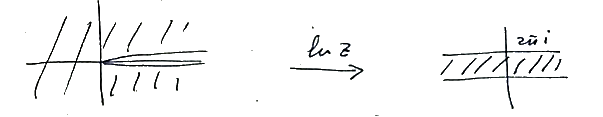
\includegraphics[width=14cm, height=3cm]{exponenta 7/log.png}
\par\bigskip
и т.д.



\section{Тригонометрические и гиперболические функции. Свойства и конформные отображения.}
\subsection{Тригонометрические функции.}
Тригонометрические функции $\sin{z}$, $\cos{z}$ определяются следующими формулами:
\[ \sin{z}=\frac{e^{iz}-e^{-iz}}{2i}; \quad \cos{z}=\frac{e^{iz}+e^{-iz}}{2}\]

Основные свойства $\sin{z}$, $\cos{z}$:
\begin{enumerate}
    \item $\sin{z}$ и $\cos{z}$ непрерывны на $\mathbb{C}$.
    \item $\sin{z}$ и $\cos{z}$ принимают все комплексные значения, то есть уравнения $\sin{z}=a$ и $\cos{z}=a$ имеют решения $\forall a \in \mathbb{C}$.
    
    В частности, отсюда следует, что $\sin{z}$ и $\cos{z}$ неограничены в $\mathbb{C}$.
    \item Все формулы элементарной тригонометрии, справедливые для действительного аргумента, имеют место и для комплексных значений. В частности, функции $\sin{z}$ и $\cos{z}$ периодичны с периодом $2\pi i$.
    \[
        \cos^2{z} + \sin^2{z} = 1; \quad \sin{2z} = 2\sin{z}\cos{z}    
    \]
    \item $\sin{z} = \sin(x+iy) = \sin{x}\cos{iy}+\cos{x}\sin{iy} = \sin{x}\ch y + i\cos x \sh y$

    $\cos z = \cos(x+iy) = \cos x \ch y - i\sh x \sh y$
    \item Связь тригометрических и гиперболических функций
    
    $\begin{aligned}[t]
        &\sin z  = -i\sh iy & &\cos z  = \ch iz\\
        &\sin iz = i\sh z   & &\cos iz = \ch z
    \end{aligned}
    $
    \item $\displaystyle \tg z = \frac{\sin z}{\cos z}, \quad \ctg z = \frac{\cos z}{\sin z}$
\end{enumerate}
\subsection{Гиперболические функции.}
Гиперболические функции $\sh z$, $\ch z$, $\th z$, $\cth h$ определяются следующими формулами:
\[ \sh{z}=\frac{e^{z}-e^{-z}}{2}; \quad \ch{z}=\frac{e^{z}+e^{-z}}{2} \]
\[ \th z = \frac{\sh z}{\ch z}; \quad \cth z = \frac{\ch z}{\sh z} \]
Для них справедливы те же формулы, что и для действительного аргумента. В частности,
\[ \ch^2 z - \sh^2 z = 1\].




\section{Обратные тригонометрические и гиперболические функции. Выражение их через логарифм.}
Определяются, как функции обратные к соответствующим тригонометрическим функциям. Рассмотрим, например, $w=\Arcsin z$

Для этого рассмотрим функцию $w=\sin z$
\begin{gather*}
    w=\frac{e^{iz}-e^{-iz}}{2i}, \quad e^{iz} = \tau \\
    2iw = \tau - \frac{1}{\tau} \Rightarrow \tau^2 - 2iw\tau - 1 = 0 \\
    \tau^2 - 2iw\tau + (iw)^2 + w^2 - 1 = 0 \\
    (\tau - iw)^2 = 1 - w^2 \\
    \tau - iw = \sqrt{1 - w^2} \\
    \tau = iw + \sqrt{1 - w^2} \Rightarrow e^{iz} = iw + \sqrt{1 - w^2} \Rightarrow \\
    z = -i\Ln \left(iw + \sqrt{1 - w^2} \right)
\end{gather*}
Переобозначив, получим:
\begin{equation*}
    \boxed{\Arcsin z = -i\Ln \left(iz + \sqrt{1 - z^2} \right)}
\end{equation*}
Аналогично: 
\begin{equation*}
    \boxed{\Arccos z = -i\Ln \left(z + \sqrt{z^2 - 1} \right)}
\end{equation*}

\begin{gather*}
    w=\cos{z}=\frac{e^{iz}+e^{-iz}}{2}, \quad e^{iz} = \tau \\
    2w = \tau - \frac{1}{\tau} \Rightarrow \tau^2 - 2w\tau + 1 = 0 \\
    (\tau - w)^2 = (w^2 - 1) \Rightarrow \\
    e^{iz} = w + \sqrt{w^2 - 1} \Rightarrow \\
    z = -i\Ln \left(w + \sqrt{w^2 - 1} \right)
\end{gather*}

\begin{equation*}
    \boxed{\Arctg z = \frac{1}{2i} \Ln \left( \frac{1 + iz}{1 - iz} \right)}
\end{equation*}

\begin{gather*}
    w=\tg{z}=\frac{\sin z}{\cos z} = \frac{e^{iz} - e^{-iz}}{(e^{iz} + e^{-iz})i}, \quad e^{iz} = \tau \\
    iw = \frac{\tau^2 - 1}{\tau^2 + 1} \Rightarrow \tau^2 - 1 = iw\tau^2 + iw \Rightarrow \\
    (1 - iw)\tau^2 - iw - 1 = 0 \Rightarrow \tau^2 = \frac{1 + iw}{1 - iw} \\
    e^{2iz} = \frac{1 + iw}{1 - iw} \Rightarrow z = \frac{1}{2i} \Ln \left( \frac{1 + iw}{1 - iw} \right)
\end{gather*}

\begin{equation*}
    \boxed{\Arcctg z = -\frac{1}{2i} \Ln \left( \frac{iz + 1}{iz - 1} \right)}
\end{equation*}

\begin{gather*}
    w=\tg{z}=\frac{\cos z}{\sin z} = i\frac{(e^{iz} + e^{-iz})}{e^{iz} - e^{-iz}}, \quad e^{2iz} = \tau \\
    -iw = \frac{\tau + 1}{\tau - 1} \Rightarrow \tau(1 + iw) = iw - 1\\
    e^{2iz} = \frac{iw - 1}{iw + 1} \Rightarrow z = \frac{1}{2i} \Ln \left( \frac{iw - 1}{iw + 1} \right)
\end{gather*}
Точно так же обратные гиперболические:
\begin{align*}
    \Arsh z &= \Ln \left( z + \sqrt{z^2 + 1} \right) \\
    \Arch z &= \Ln \left( z + \sqrt{z^2 - 1} \right) \\
    \Arcth z &= \frac{1}{2} \Ln \left( \frac{1 + z}{1 - z} \right) \\
    \Arccth z &= \frac{1}{2} \Ln \left( \frac{z + 1}{z - 1} \right)
\end{align*}
Все вышеупомянутые функции являются многозначными, поэтому можно рассматривать главные ветви этих функций, которые получаются выбором главных ветвей функций $\Ln z$ и $\sqrt z$.






\section{Дифференциируемость ФКП}
Понятие дифференциируемости функции комплексного переменного вводится аналогично понятию дифференциируемости действительной функции.
\par\bigskip
Пусть функция $f$ определена, однозначна и конечна в окрестности \textsl{U($z_0$)} точки $z_0 \in \mathbb{C}$. 
\par Функцию $f$ называют \textbf{дифференциируемой в точке} $z_0$, если существует такое С $\in \mathbb{C}$,
\par что:
\par\bigskip
\begin{center}
$\forall \Delta z, z_0 + \Delta z \in \textsl{U($z_0$)} \Rightarrow \textsl{f} (z_0 + \Delta z) = \textsl{f} (z_0) + C\Delta z + \alpha(\Delta z)|\Delta z|$.
\end{center}
\par\bigskip
где С - комплексное число, $\alpha (\Delta z) \to 0$ при $\Delta z \to 0, \alpha (0) = 0$.
\par
Число С называют \textbf{производной функции} $f$ в точке $z_0$.
\par
Производную функции обозначают любым из следующих способов:
\par\bigskip
\begin{center}
\textsl{f'}($z_0$), $\frac{\textsl{df}(z_0)}{\textsl{d}z}$,
$\left. \frac{\textsl{df}(z)}{\textsl{d}z} \right |_{z=z_0}$
\end{center}
\par\bigskip
Выражение С$\Delta z$ называют \textbf{дифференциалом} $\textsl{df}(z_0)$ функции $f$ в точке $z_0$.
\newline
Из определения дифференциала следует, что дифференциал независимой переменной $z$ совпадает с приращением этой переменной. Поэтому $dz$ = $\Delta z$ для независимой переменной $z$, и дифференциал функции $f$ в точке $z_0$ равен $f'(z_0)dz$, таким образом:
\par\bigskip
\begin{center}
$df$ = $f'(z_0)\,dz$
\end{center}
\par\bigskip
Из определения производной следует, что производную функции в точке можно вычислить как предел отношения приращения функции к приращению аргумента, когда последний стремится к нулю:
\par\bigskip
\begin{center}
$ \lim_{\Delta z \to 0} \frac{\textsl{f} (z_0 + \Delta z) - \textsl{f} (z_0)}{\Delta z} = \lim_{\Delta z \to 0} \frac{C\Delta z + \alpha(\Delta z)|\Delta z|}{\Delta z} = C = \textsl{f'}(z_0)$
\end{center}
\bigskip
Верно и обратное утверждение:
\par\bigskip
\textbf{Теорема.} \hspace{2 mm}
\textsl{Если существует конечный предел }
\par\bigskip
\begin{center}
$ \lim_{\Delta z \to 0} \frac{\textsl{f} (z_0 + \Delta z) - \textsl{f} (z_0)}{\Delta z} = C$.
\end{center}
\par\bigskip
\textsl{то функция $f$ дифференциируема в точке $z_0$ и её производная $f'(z_0)$ = С.}
\par\bigskip
$\blacklozenge$\; Из существования предела следует, что 
\par\bigskip
\begin{center}
$\frac{\textsl{f} (z_0 + \Delta z) - \textsl{f} (z_0)}{\Delta z} = C + \alpha_1(\Delta z)$
\end{center}
\par\bigskip
где $\alpha_1(\Delta z) \to_{\Delta z \to 0} 0$, откуда
\par\bigskip
\begin{center}
$\textsl{f} (z_0 + \Delta z) - \textsl{f} (z_0) = C\Delta z + \alpha_1(\Delta z)\Delta z$
\end{center}
\par\bigskip
Полагая
\par\bigskip
\begin{center}
$\alpha (\Delta z) = \begin{cases}
\frac{\alpha_1 (\Delta z)\Delta z}{|\Delta z|},$ при  $ \Delta z \not= 0,\\
  0, $ при $ \Delta z = 0.
\end{cases}$
\end{center}
\par\bigskip
Получаем
\par\bigskip
\begin{center}
$\textsl{f} (z_0 + \Delta z) = \textsl{f} (z_0) + C\Delta z + \alpha(\Delta z)|\Delta z|$
\end{center}
\par\bigskip
где $\alpha (\Delta z) \to 0 $ при $\Delta z \to 0$, $\alpha (0) = 0.$ Полученное равенство, в силу определения,
\par\bigskip
и означает дифференциируемость функции $f$ в точке $z_0$. \quad
$\blacksquare$

\par\bigskip
Таким образом, дифференциируемость функции $f$ в точке $z_0$ равносильна существованию конечного предела отношения приращения функции в этой точке к приращению аргумента, когда приращение аргумента стремится к нулю.
\par
Из определения дифференциируемоти вытекает, что функция, дифференциируемая в точке, является непрерывной в этой точке.
\par
На ФКП распространяются все правила дифференциирования функций действительного аргумента. Имеют место следующие утверждения:

\par\bigskip
\textbf{Теорема.} \quad
\textsl{Если функции $f$ и $g$ - дифференциируемы в точке $z_0$, то дифференциируемыми в этой точке так же являются:}
\par
\textsl{1) линейная комбинация функций $f$ и $g$ с любыми комплексными коэффицентами a и b, при этом: }
\par\bigskip
\begin{center}
    $\left. (af(z) + bf(z))' \right |_{z=z_0} = af'(z_0) + bf'(z_0);$
\end{center}
\par\bigskip
\textsl{2) произведение $f(z)g(z)$ функций $f$ и $g$, при этом:}
\par\bigskip
\begin{center}
 $\left. (f(z)g(z))' \right |_{z=z_0} = f'(z_0)g(z_0) + f(z_0)g'(z_0);$
\end{center}
\par\bigskip
\textsl{3) частное $f(z)/g(z)$ функций $f$ и $g$ со знаменателем отличным от нуля, при этом:}
\par\bigskip
\begin{center}
 $\left. (f(z)/g(z))' \right |_{z=z_0} = \frac{f'(z_0)g(z_0) - f(z_0)g'(z_0)}{g^2(z_0)};$
\end{center}

\section{Условия Коши-Римана}
Непрерывность функции $f$ равносильна непрерывности её действительной и мнимой частей. Но для дифференциируемости функции $f$ не достаточно диффференциируемости ей действительной и мнимой частей. Имеет место следующая теорема:
\par\bigskip
\textbf{Теорема.} \quad
\textsl{Для того, чтобы функция $f(z) = u(x, y) + iv(x, y)$, заданная в окрестности точки $z = x + iy$, была дифференцируемой в точке $z$, необходимо и достаточно выполнение следующих условий: }
\par\bigskip
\textsl{1) функции $u(x, y)$ и $v(x, y)$ дифференцируемы в точке $(x, y)$}
\par
\textsl{2) в точке $(x, y)$ выполнены условия \textbf{Коши-Римана}:}
\par\bigskip
\begin{center}
$\frac{\partial u(x, y)}{\partial x} = \frac{\partial v(x, y)}{\partial y}$ \quad $ \frac{\partial u(x, y)}{\partial y} = -\frac{\partial v(x, y)}{\partial x}$ 
\quad(1)
\end{center}
\par\bigskip
\textsl{При выполнении уловия теоремы производная функции f может быть вычислена по любой из следующих формул:}
\par\bigskip
\begin{center}
$f'(z) = \frac{\partial u(x, y)}{\partial x} + i\frac{\partial v(x, y)}{\partial x}.$ \quad $ f'(z) = \frac{\partial v(x, y)}{\partial y} - i\frac{\partial u(x, y)}{\partial y}$ , 
\par\bigskip
$f'(z) = \frac{\partial u(x, y)}{\partial x} - i\frac{\partial u(x, y)}{\partial y}.$ \quad  $ f'(z) = \frac{\partial v(x, y)}{\partial y} + i\frac{\partial v(x, y)}{\partial x}$  (2)
\end{center}
\par\bigskip
$\blacklozenge \Rightarrow )$ Пусть функция $f$ дифференцируема в точке $z = x + iy$. Тогда 
\par\bigskip
\begin{center}
    $\Delta f = f(z + \Delta z) - f(z) = f'(z)\Delta z + \alpha (\Delta z)|\Delta z|$.  (3)
\end{center}
\par\bigskip
где $\alpha(\Delta z) \to_{\Delta z \to 0} 0, \alpha (0) = 0$.
\par
Приращение $\Delta f(z)$ может быть представлено в виде: 
\par\bigskip
\begin{center}
    $\Delta f(z) = \Delta u(x, y) + i\Delta v(x, y).$
\end{center}
\par\bigskip
Положим
\par\bigskip
\begin{center}
    $f'(z) = A + iB, \rho = |\Delta z| = \sqrt{\Delta x^2 + \Delta y^2}$.
    \par\bigskip
    $\alpha (\Delta z) = \alpha_1 (\Delta x, \Delta y) + i\alpha_2 (\Delta x, \Delta y).$
\end{center}
\par\bigskip
причём
\par\bigskip
\begin{center}
   $\underset{\Delta x \to 0, \Delta y \to 0}{lim} \alpha_1 (\Delta x, \Delta y) = \underset{\Delta x \to 0, \Delta y \to 0}{lim} \alpha_2 (\Delta x, \Delta y) = 0$.
   \par\bigskip
   $\alpha_1(0, 0) = \alpha_2(0,0) = 0$.
\end{center}
\par\bigskip
Тогда (3) примет вид:
\par\bigskip
\begin{center}
   $\Delta u(x, y) + i\Delta v(x, y) = (A + iB)(\Delta x + i\Delta y) + (\alpha_1 (\Delta x, \Delta y) + i\alpha_2 (\Delta x, \Delta y))\rho.$
\end{center}
\par\bigskip
Что равносильно системе:
\par\bigskip
\begin{center}
   $\begin{cases}
    \Delta u(x, y) = A\Delta x - B\Delta y + \alpha_1 (\Delta x, \Delta y)\rho \\
    \Delta v(x, y) = A\Delta y + B\Delta x + \alpha_2 (\Delta x, \Delta y)\rho
    \end{cases}$
\end{center}
\par\bigskip
которая и означает дифференциируемость $u $ и $ v$ в точке $(x, y)$.
\par 
Из этой системы вытекает, что:
\par\bigskip
\begin{center}
   $A = \frac{\partial u}{\partial x}, -B = \frac{\partial u}{\partial y},$
   \par\bigskip
   $ A = \frac{\partial v}{\partial y}, B = \frac{\partial v}{\partial x}.$
\end{center}
\par\bigskip

откуда и следует (1). Т.к. $f'(z) = A + iB$, то из этих же равенств следует (2) для производной функции $f$.
\par
$\Leftarrow$) Так как функции $u$ и $v$ дифференциируемы в точке $(x, y)$, то для них выполнены равенства:
\par\bigskip
\begin{center}
   $\begin{cases}
    \Delta u(x, y) = \frac{\partial u(x, y)}{\partial x}\Delta x + \frac{\partial u(x, y)}{\partial y}\Delta y + \alpha_1 (\Delta x, \Delta y)\rho \\
    \Delta v(x, y) = \frac{\partial v(x, y)}{\partial x}\Delta x + \frac{\partial v(x, y)}{\partial y}\Delta y + \alpha_2 (\Delta x, \Delta y)\rho
    \end{cases}$
\end{center}
\par\bigskip
где 
\par\bigskip
\begin{center}
  $\underset{\Delta x \to 0, \Delta y \to 0}{lim} \alpha_1 (\Delta x, \Delta y) = \underset{\Delta x \to 0, \Delta y \to 0}{lim} \alpha_2 (\Delta x, \Delta y) = 0$.
   \par\bigskip
   $\alpha_1(0, 0) = \alpha_2(0,0) = 0$.
\end{center}
\par\bigskip
Из выполнения условий Коши-Римана (1) следует, что 
\par\bigskip
\begin{center}
   $\begin{cases}
    \Delta u(x, y) = \frac{\partial u(x, y)}{\partial x}\Delta x - \frac{\partial v(x, y)}{\partial x}\Delta y + \alpha_1 (\Delta x, \Delta y)\rho \\
    \Delta v(x, y) = \frac{\partial v(x, y)}{\partial x}\Delta x + \frac{\partial u(x, y)}{\partial x}\Delta y + \alpha_2 (\Delta x, \Delta y)\rho
    \end{cases}$
\end{center}
\par\bigskip
Умножая второе равенство на $i$ и складывая с первым получим:
\par\bigskip
\begin{center}
   $\Delta u(x, y) + i\Delta v(x, y) = \left (\frac{\partial u(x, y)}{\partial x} + i\frac{\partial v(x, y)}{\partial x} \right )\Delta x - \left (\frac{\partial v(x, y)}{\partial x} - i\frac{\partial u(x, y)}{\partial x} \right )\Delta y +$
   \par\bigskip
   $ + (\alpha_1 (\Delta x, \Delta y) + i \alpha_2 (\Delta x, \Delta y))\rho$,
\end{center}
\par\bigskip
откуда 
\par\bigskip
\begin{center}
$\Delta u(x, y) + i\Delta v(x, y) = \left (\frac{\partial u(x, y)}{\partial x} + i\frac{\partial v(x, y)}{\partial x} \right )(\Delta x + i\Delta y) +$
\par\bigskip
   $ + (\alpha_1 (\Delta x, \Delta y) + i\alpha_2 (\Delta x, \Delta y))\rho$.
\end{center}
\par\bigskip
Поэтому
\par\bigskip
\begin{center}
$\Delta f(z) = \left (\frac{\partial u(x, y)}{\partial x} + i\frac{\partial v(x, y)}{\partial x} \right )(\Delta x + i\Delta y)\Delta z + \alpha (\Delta z)|\Delta z|$, 
\end{center}
\par\bigskip
где функция $\alpha (\Delta z) = \alpha_1 (\Delta x, \Delta y) + i\alpha_2(\Delta x, \Delta y)$ удоволетворяет условиям
\par\bigskip
\begin{center}
$\underset{\Delta z \to 0}{lim} \alpha (\Delta z) = 0,  \alpha (0) = 0$,
\end{center}
\par\bigskip
что и означает дифференциируемость функции $f$ в точке $z$ и выполнение равенства
\par\bigskip
\begin{center}
    $f'(z) = \frac{\partial u(x, y)}{\partial x} + i\frac{\partial v(x, y)}{\partial x}.$
\end{center}
\par\bigskip
Из этой формулы с помощью условий Коши-Римана (1) получаются остальные формулы (2) для производной $f'$ функции $f$.




\section{Сопряженные гармонические функции}
Выясним, может ли произвольная действительная функция $u(x,y)$, дифференцируемая в точке $(x,y)$, быть действительной (или мнимой) частью некоторой дифференцируемой функции $f(z)$.
\par\bigskip
Пусть $f(z) = u(x, y) + iv(x, y)$ дифференцируема в точке $z = (x + iy)$ и $u$ и $v$ имеют непрерывные частные производные до 2-ого порядка включительно. Тогда из условия Коши--Римана имеем
\begin{center}
    $\dfrac{\partial u}{\partial x} = \dfrac{\partial v}{\partial y}; \quad \dfrac{\partial u}{\partial y} = -\dfrac{\partial v}{\partial x}$
\end{center}
Дифференцируя по $x$ и $y$, получаем
\begin{center}
    $\dfrac{\partial^2 u}{\partial x^2} = \dfrac{\partial^2 v}{\partial x \partial y}; \quad \dfrac{\partial^2 u}{\partial y^2} = -\dfrac{\partial^2 v}{\partial y \partial x}$
\end{center}
Учитывая, что 
\begin{center}
    $\dfrac{\partial^2 v}{\partial x \partial y} = \dfrac{\partial^2 v}{\partial y \partial x}$
\end{center}
Получаем 
\begin{center}
    $\dfrac{\partial^2 u}{\partial x^2} + \dfrac{\partial^2 u}{\partial y^2} = \Delta u = 0$
\end{center}
Аналогично получаем
\begin{center}
    $\dfrac{\partial^2 v}{\partial x^2} + \dfrac{\partial^2 v}{\partial y^2} = \Delta v = 0$
\end{center}
Следовательно, функции $u$ и $v$ должны удовлетворять условию Лапласа.

\par\bigskip
Функции, которые удовлетворяют уравнению Лапласа и дважды непрерывно дифференцируемы, называются \textbf{гармоническими функциями.}
\par\bigskip
Действительная и мнимая части дифференцируемой ФКП являются гармоническими функциями.
\par\bigskip
Гармонические функции $u(x, y)$ и $v(x, y)$, связанные между собой условиями Коши-Римана, называются \textbf{сопряженными}.
\par\bigskip
Таким образом, действительная и мнимая части дифференцируемой в области $D$ функции являются в этой области сопряженными гармоническими функциями. 
\par\bigskip
Верно и обратное: Если в области $D$ есть две сопряженные гармонические функции $u(x, y)$ и $v(x, y)$, то функция $f(z) = u + iv$ дифференцируема в обсласти $D$. Это следует из критерия дифференцируемости.
\par\bigskip

\textbf{Теорема.} \quad
\textit{Функция $f(z) = u + iv$ дифференцируема в области $D \quad \Longleftrightarrow \quad u(x, y)$ и $v(x, y)$ являются сопряженными гармоническими в этой области.}
\par\bigskip

Зная одну из сопряженных гармонических функций $u(x, y)$ или $v(x, y)$, всегда можно восстановить и другую.
\par\bigskip

\textbf{Теорема.} \quad
\textit{Для всякой функции $u(x, y)$, гармонической в односвязной области $D$, можно найти сопряженную с ней гармоническую функцию, определяемую с точностью до произвольного постоянного слагаемого.}
\newline 
$\blacklozenge$ \hspace{1 mm} Т.к. $u(x, y)$ $-$ гармоническая в области $D$, то имеет место уравнение:
\begin{center}
    $\dfrac{\partial}{\partial y}(-\dfrac{\partial u}{\partial y}) = \dfrac{\partial}{\partial x}(\dfrac{\partial u}{\partial x})$
\end{center}
И, следовательно, выражение
\begin{center}
    $-\dfrac{\partial u}{\partial y}dx + \dfrac{\partial u}{\partial x}dy = Pdx + Qdy$
\end{center}
является полным дифференциалом некоторой однозначной функции $v(x, y)$, определяемой формулой 
\begin{center}
    $$v(x, y) = \int\limits_{(x_0, y_0)}^{(x, y)} -\dfrac{\partial u}{\partial y}dx + \dfrac{\partial u}{\partial x}dy\ + C \eqno (1)$$
\end{center}
Из $(1)$ имеем
\begin{center}
    $\dfrac{\partial v}{\partial x} = -\dfrac{\partial u}{\partial y};\quad \dfrac{\partial v}{\partial y} = \dfrac{\partial u}{\partial x} $
\end{center}
Откуда следует, что $v(x, y)$ -- гармоническая в области $D$ функция, сопряженная с $u(x, y)$.
$\blacksquare$
\par\bigskip

На практике, при восстановлении функции $f$ иногда удобнее вычисление криволинейного интеграла заменить на использование условия Коши--Римана.
\par\bigskip

\textbf{Пример.}\quad Найти $f(z)$, если $u(x, y) = y^3 - 3x^2y$ и $f(0) = 0$
\par\bigskip
\textit{1 способ}
\par
по формуле $(1)$
\begin{center}
    $v(x, y) = \int\limits_{(0, 0)}^{(x, y)} (-3y^2 + 3x^2)dx - 6xydy = \int\limits_0^x 3x^2\,dx - \int\limits_0^y 6xy\,dy = x^3 - 3xy^2 + C $
\end{center}
\begin{center}
    $f(z) = y^3 - 3x^2y + ix^3 - 3ixy^2 + Ci = i(x^3 + 3x^2yi + 3xy^2 + i^3y^3) + iC = i(x + iy)^3 + iC = iz^3 + iC$
    
\end{center}
\par
И т.к. $f(0) = 0$ \quad => \quad $f(z) = iz^3$
\par\bigskip
\textit{2 способ}
\par\bigskip
\begin{center}
    $-\dfrac{\partial u}{\partial x} = \dfrac{\partial v}{\partial y} = -6x y \quad => \quad v(x, y) = -3x y^2 + \varphi(x)$
\end{center}
\par\bigskip
\begin{center}
    $\dfrac{\partial v}{\partial x} = -3y^2 + \varphi'(x) = -\dfrac{\partial u}{\partial y} = -3y^2 + 3x^2 \quad => \quad \varphi'(x) = 3x^2 \quad => \quad \varphi(x) = x^3 + C$
    \par\bigskip
    $v = -3xy^2 + x^3 + C$
\end{center}


\newpage
\section{Геометрический смысл производной аргумента ФКП}
Пусть функция $w = f(z)$ дифференцируема в некоторой окрестности точки $z_0$, и пусть $f'(z_0) \not= 0$. Рассмотрим в плоскости гладкую кривую $l$, уравнение которой $z = \sigma (t)$, $\alpha \le t \le \beta$, проходящую через точку $z_0$, $z_0 = \sigma(t_0)$, $t_0 \in ]\alpha, \beta[$.
\begin{figure}[bh]
\begin{minipage}[t]{0.32\linewidth}
\center{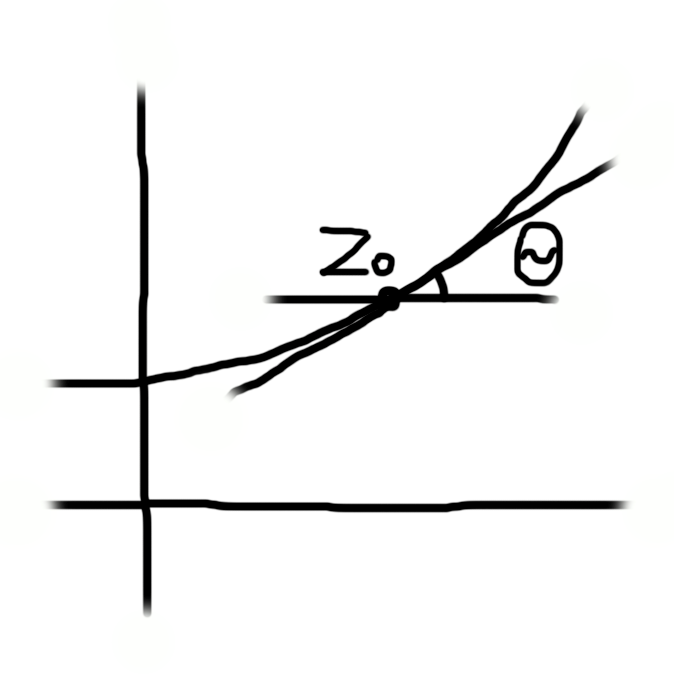
\includegraphics[width=0.8\linewidth]{geom fkp 13-14/2.png}}
\end{minipage}
\hfill
\begin{minipage}[t]{0.32\linewidth}
\center{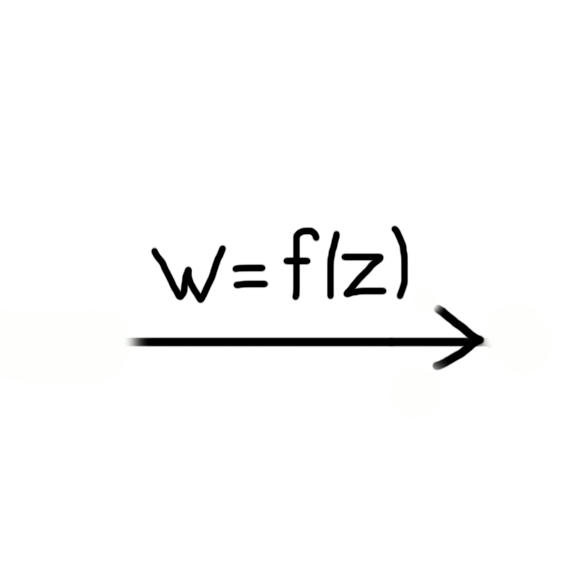
\includegraphics[width=0.8\linewidth]{geom fkp 13-14/3.png}}
\end{minipage}
\hfill
\begin{minipage}[t]{0.32\linewidth}
\center{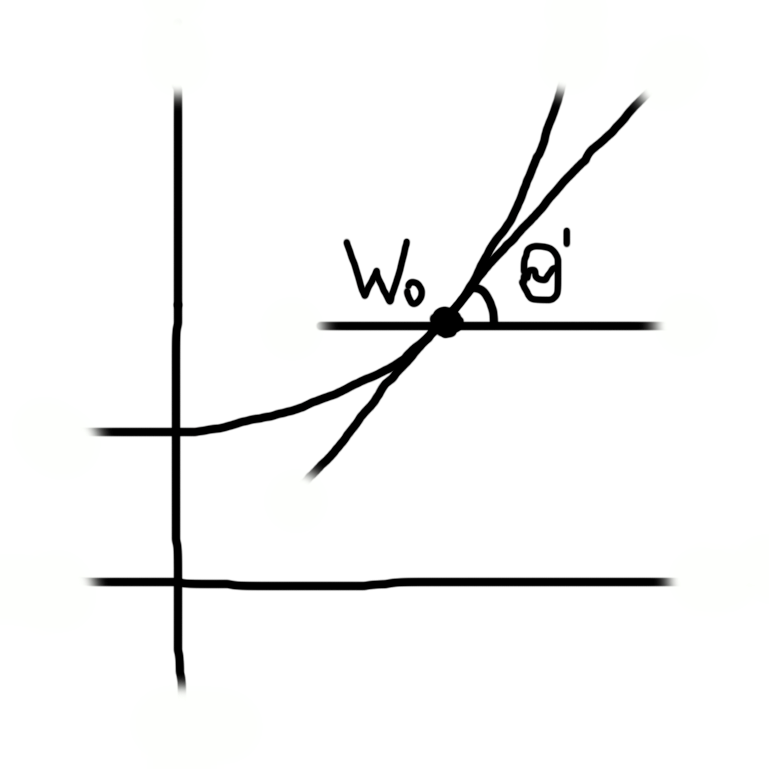
\includegraphics[width=0.8\linewidth]{geom fkp 13-14/1.png}}
\end{minipage}
\end{figure}
Обозначим через $\theta$ угол, образуемый кривой $l$ в точке $z_0$ с положительным направлением действительной оси, т.е. $\theta$ - угол между $Ox$ и касательной. 
\par Тогда, как нам уже известно
\begin{center}
    $\theta = arg \, \sigma'(t_0)$
\end{center}
\par Функция $f$ отображает окрестность точки $z_0$ на некоторую окрестность точки $w_0 = f(z_0)$ плоскости $w$, и при этом $l \rightarrow L$, т.е. $L = f(l)$. 
\par Мы можем написать уравнение $L$:
\begin{center}
    $w = w(t) = (f \circ \sigma)(t) = f(\sigma(t)), \quad \alpha \le t \le \beta$
\end{center}
\par По правилу дифференцирования композиций
\begin{center}
    $$w'(t_0) = f'(\sigma(t_0)) \cdot \sigma'(t_0) = f'(z_0)\sigma'(t_0)  , \quad \alpha \le t \le \beta \eqno(*)$$
\end{center}
\par\bigskip Т.к. кривая $l$ гладкая, и поэтому $\sigma'(t_0) \not= 0$, a $f'(z_0) \not= 0$ по условию, то из $(*)$ следует, что $w'(t_0) \not= 0$, что означает гладкость кривой $L$ в точке $w_0$. Поэтому в точке $w_0$ существует касательная к $L$.
\par Обозначим угол, образованный касательной к кривой $L$ и положительным направлением оси $Ox$ через $\theta'$:
\begin{center}
    $\theta' = arg \, w'(t_0)$
\end{center}
\par Из $(*)$ вытекает, что 
\begin{center}
    $\theta' = arg \, w'(t_0) = arg \, f'(z_0) + arg \, \sigma'(t_0)$
\end{center}
\par Обозначим $\alpha := arg \, f'(z_0)$
\par Тогда предыдущее равенство перепишем в виде
\begin{center}
    $\theta' = \alpha + \theta$ \quad или \quad $\theta' - \theta = \alpha$ 
\end{center}
\par Величина $\theta' - \theta$ называется \textbf{углом поворота кривой} $l$ в точке $z_0$ при отображении $w = f(z)$.
\par\bigskip
Из рассмотренного видно, что если $f'(z_0) \not= 0$, то угол поворота в точке $z_0$ не зависит от вида и направления кривой и равен $\alpha = arg \, f'(z_0)$.
\par Это означает, что все кривые, проходящие через точку $z_0$, поворачиваются при отображении $w = f(z)$ на один и тот же угол, равный аргументу производной в точке $z_0$.
\par\bigskip Таким образом, отображение $w = f(z)$, где $f$ дифференцируемая в окрестности точки $z_0$ функция и $f'(z_0) \not= 0$ сохраняет углы между кривыми, проходящими через точку $z_0$, не только по величине, но и по направлению отсчёта.
\begin{figure}[t]
\begin{minipage}[t]{0.32\linewidth}
\center{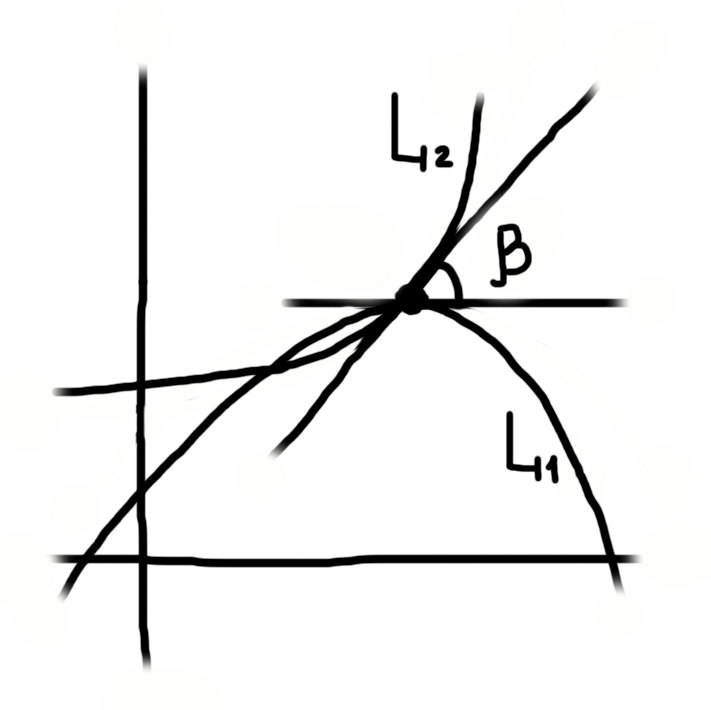
\includegraphics[width=0.8\linewidth]{geom fkp 13-14/4.png}}
\end{minipage}
\hfill
\begin{minipage}[t]{0.32\linewidth}
\center{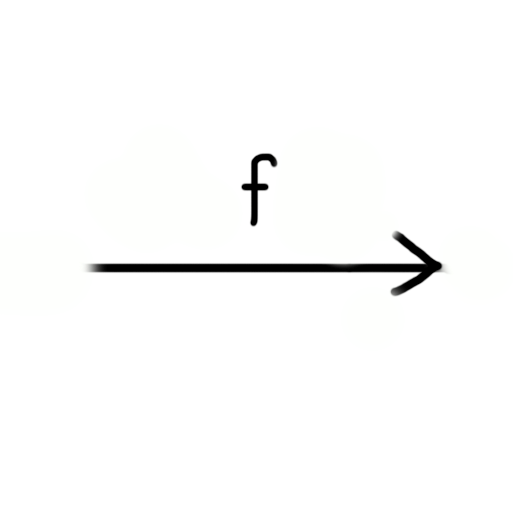
\includegraphics[width=0.8\linewidth]{geom fkp 13-14/5.png}}
\end{minipage}
\hfill
\begin{minipage}[t]{0.32\linewidth}
\center{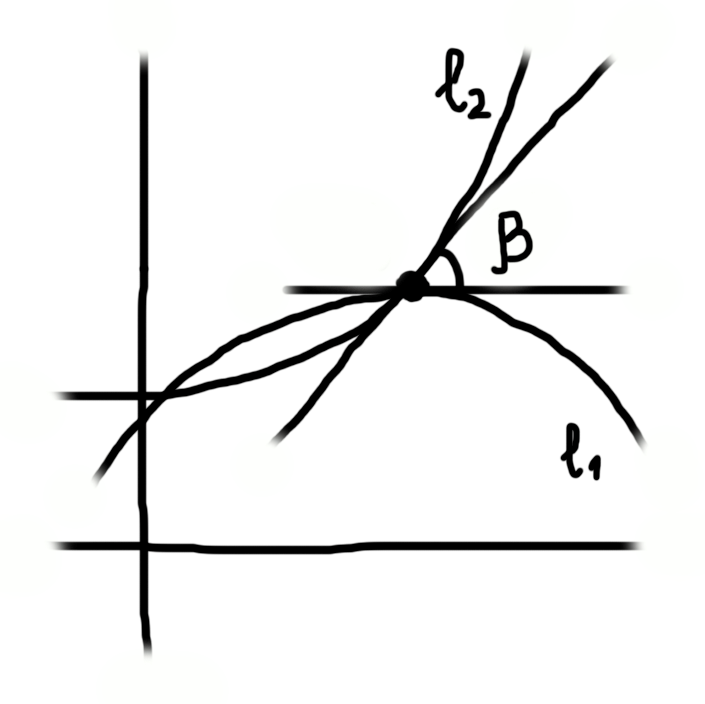
\includegraphics[width=0.8\linewidth]{geom fkp 13-14/6.png}}
\end{minipage}
\end{figure}





\par\bigskip Рассмотрим теперь в прежних предположениях ($f$ - дифференцируема в т. $z_0$\\ и $f'(z_0) \ne 0$) произвольную точку $z = z_0 +\Delta z$, расположенную в достаточно малой окрестности т. $z_0$.

Тогда $\Delta w = f(z_0 + \Delta z) - f(z_0) = w - w_0 \quad \Rightarrow \quad w = w_0 + \Delta w$.

Известно, что $f'(z_0) = \lim\limits_{\Delta z \rightarrow 0} \dfrac{\Delta w}{\Delta z}$. Отсюда вытекает:

\begin{center}
	$\lim\limits_{|\Delta z \rightarrow 0|} \dfrac{\Delta w}{\Delta z} = |f'(z_0)|$
	\bigskip

	или $|\Delta w| = |f'(z_0)||\Delta z| + o(|\Delta z|)$
\end{center}

Пусть $|z - z_0| = \rho$, где $\rho$ - $fix$ и достаточно мало. Тогда последняя формула говорит, что:
	$$|\Delta w| = |f'(z_0)|\rho + o(|\Delta z|)$$
	\par\bigskip
Другими словами, окружность $|z - z_0| = \rho$ при отображении $f$ переходит в замкнутую кривую, которая мало отличается от окружности $|w - w_0| = |\Delta w| = \rho \cdot |f'(z_0)| + o(|\Delta z|)$

Иначе говоря, отображение $f$ с точностью до бесконечно малых более высокого порядка, чем $|\Delta z|$, растягивает круг $|\Delta z| \leq \rho$ в $|f'(z_0)|$ раз.

Величина $\lim\limits_{\Delta z \rightarrow 0}\dfrac{\Delta w}{\Delta z} = k$ называется \textbf{коэффициентом линейного растяжения} элемента $z - z_0 = \Delta z$ в точке $z_0$ при отображении $w = f(z)$.
\par\bigskip 
Таким образом, линейное растяжение в точке $z_0$ не зависит от положения элемента $z_0 +\Delta z$ и всегда равно $f'(z_0)$ ($f$ - дифференцируема и $|f'(z_0)| \ne 0$). Это свойство называют \textbf{свойством постоянства расстояния}.

\begin{center}
    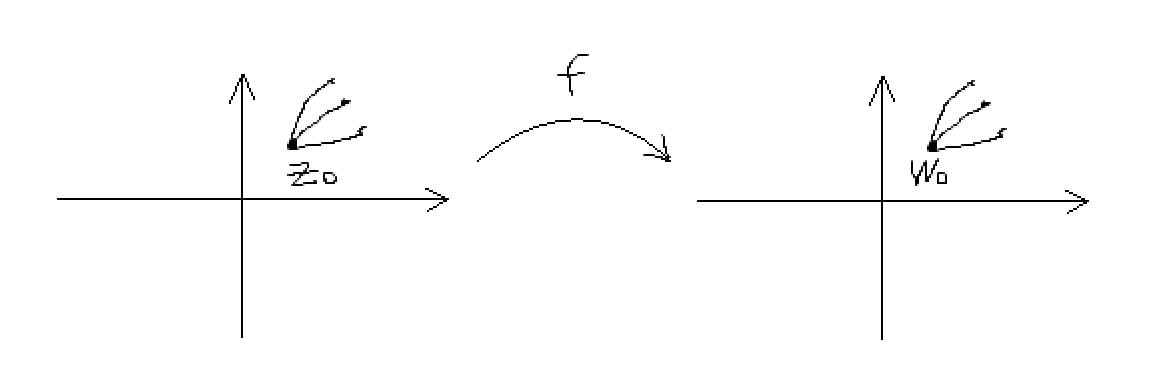
\includegraphics[width=15 cm]{zInF.png}
\end{center}

	
\par\bigskip
\section{Конформные отображения}

\par Пусть $f: D \rightarrow C, D \in C$.
\par\bigskip
Отображение $f$ называют \textbf{конформным в точке $z_0 \in D$}, если оно сохраняет угол между кривыми и обладает постоянством расстояний.
\par\bigskip
Геометрический смысл производной говорит о том, что есть $f$ дифференцируемая в некоторой окрестности точки $z_0 = f'(z_0) \ne 0$, то отображение $w = f(z)$ является конформным в точке $z_0$.

Отметим, что условие $f'(z) \ne 0$ является существенным. Оно означает, что Якобиан отображения отличен от нуля. Действительно, отображение $w = f(z)$ можно трактовать как действительное отображение:
\begin{center}
	\begin{cases}
	    u = u(x, y)
	    \\
	    v = v(x, y)
	\end{cases}
\end{center}

области $D$ на некоторой область $G$. Якобиан этого отображения в точке $(x_0, y_0)$ можно выписать следующим образом:
\begin{center}
	$J(x_0, y_0) = \begin{vmatrix} \frac{\partial u}{\partial x}& \frac{\partial u}{\partial y} \\ \frac{\partial v}{\partial x}& \frac{\partial v}{\partial y} \end{vmatrix} = \frac{\partial u}{\partial x} \cdot \frac{\partial v}{\partial y} - \frac{\partial u}{\partial y} \cdot \frac{\partial v}{\partial x} = \begin{bmatrix} \frac{\partial u}{\partial x} = \frac{\partial v}{\partial y};\ \frac{\partial u}{\partial y} = -\frac{\partial v}{\partial x} \end{bmatrix} = (\frac{\partial u}{\partial x})^2 + (\frac{\partial v}{\partial x})^2 = |f'(z_0)|^2 \not= 0$
\end{center}

\par\bigskip
Если отображение взаимно-однозначно и конформно в каждой точке области $D$, то его называют \textbf{конформным в области $D$}.
\par\bigskip
Из сказанного вытекает, что если:
\begin{enumerate}
    \item $f$ - однозначны и однолистны в $D$
    \item $f$ - дифференциируема в $D$
    \item $f'(z)\ne 0 \quad \forall z \in D$
\end{enumerate}

то $f(z)$ конформно в $D$.
\par\bigskip

Иногда рассматривают конформные отображения ..., их называют конформными отображениями $2$ рода, а ... $1$
\par\bigskip

Например $w =\overline{z}$. Она не дифференциируема нигде, однако
\begin{center}
    $z=\rho e^{i\phi}$;   \quad   $ w=r\cdot e^{i\psi} \quad \Rightarrow \quad \psi = -\phi $ \quad и \quad $r = \rho$
\end{center}

Очевидно, что конформным отображением 2 рода будет и отображение $f(\overline{z})$, если $f$ обладает свойствами 1-3.
\par\bigskip
\textbf{Пример:}
\begin{enumerate}
    \item $w=\dfrac{1}{z}$, $w'=-\dfrac{1}{z^2}$ отображение конформно во всех точках (кроме м.б. $z=0$, и $z=\infty$)
    \item $w=z^2$ - конформно во всех точках пространства за исключением точки $z=0$ : $\arg w=2\arg z$
\end{enumerate}

\subsection{Вычисление площадей и длин дуг образов фигур}

Пусть $f$ дифференцируема в замыкании $\overline{D}$, ограниченной в области $D$ и $G$ - образ $D$ при отображении $w=f(z)$. $G$ также область, так как $f$ непрерывно равн. Функцию $f$ предполагаем однозначной и однолистной в области $D$ и пусть $l$-изменяемая кривая в $D$, а $L$ ее образ.
\par\bigskip

Тогда(площадь $G$) = $\iint\limits_D(|f'(z)|^2) dx\,dy$. \par(Для $L$)=$\underset{l}{\int}|f'(z)||dz|$
\\
$\blacklozenge$

\begin{enumerate}
    \item Площадь $G$=$\iint\limits_G du\,dv=\iint\limits_D(|J(x,y)|) dx\,dy=\underset{D}{\int}\int(|f'(z)|^2) dx\,dy$
    \item Пусть уравнение $l: z = \sigma(t),t\in|\alpha,\beta|$,\  $l=\int\limits_\alpha^\beta|\sigma'(t)dt|$
    \par Тогда $L: z = (f\circ \sigma)(t)=f(\sigma(t)),t\in(\alpha,\beta)$\par
    $\text{дл.}L=\int\limits_\alpha^\beta|f"(\sigma(t)|dt=\int\limits_\alpha^\beta|f'(\sigma(t)||\sigma'(t)|dt=\int\limits_\alpha^\beta|f'(Z)||\sigma(t)dt|=\int\limits_{l}|f'(z)|ds=\int\limits_{l}|f'(z)||dz|$
\end{enumerate} \blacksquare








\par\bigskip
\section{Интеграл ФКП}
\bigskip
\begin{wrapfigure}[10]{l}{0.4\linewidth} 
    
    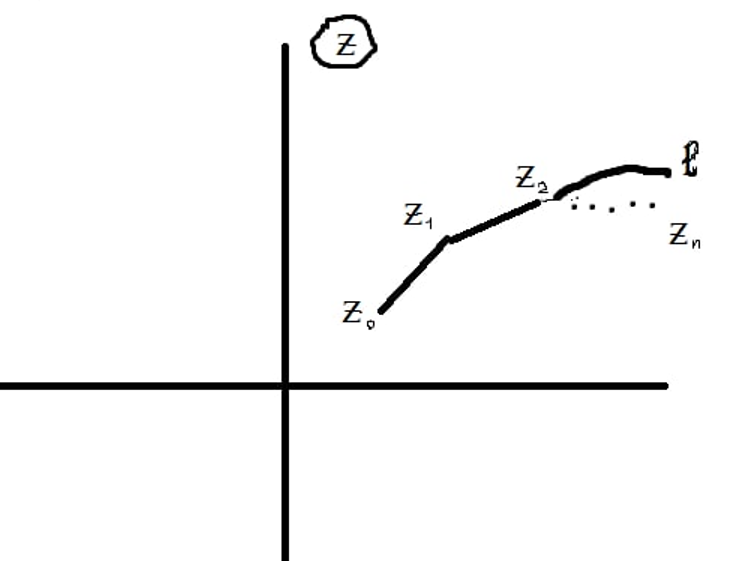
\includegraphics[width=0.4\textwidth]{123.png}
\end{wrapfigure}
Пусть на комплексной плоскости \(  Z \)  некоторая ориентированная кусочно-гладкая кривая \( l \). 
Пусть также на \(  l \) определена функция комплексного измененного \( z \)   \(w = f(z)\). Разобъем кривую l точками \( z_0, z_1, ... , z_n \), где \( z_0 \) - начало кривой, \( z_n \) - конец кривой, на n частей.
\par\bigskip
Введем обозначения:  
\item \( \Delta z_k ::= z_k - z_{k-1} \) , \( \sigma = \max | \Delta z_k| \)
\item Если  \( l_k \) - участок кривой между точками \( z_{k-1}\) и \( z_k\) , что выберем точку \( \xi_k \in l_k \) 
\par\bigskip
\textbf
\textbf{Составим интегральную сумму  \( \sigma = \sum\limits_{k=1}^n  f( \xi_k ) \Delta z_k \)}
\par\bigskip Если существует \( \lim\sigma \) и он не зависит ни от способа разбиения кривой, ни от выбора точек \( \xi_k \), то его называют \textbf{интегралом от функции} \( \textbf{f(z)} \) \textbf{по кривой} \(  \textbf{l} \) и обозначают символ \(  \int\limits_l  f(z)dz\) 
\par\bigskip
Таким образом \( \ \int\limits_l f(z)dz = \underset{\sigma \to 0}{lim}  \sum\limits_{k=1}^n  f( \xi_k ) \Delta z_k\) 
\par\bigskip
Теперь встаёт вопрос о существовании интеграла и его вычислении.
\par\bigskip
Пусть
\par \( z= x + iy\),\quad  \(  f(z)= u(x,y)+iv(x,y)\),  
\par \(  z_k=x_k+iy_k \), \quad \(  x_k-x_{k-1}= \Delta x_k\), \quad
\(  y_k-y_{k-1}= \Delta y_k\), \par  \(\xi_k =\xi_k +i\eta_k \) . (?)


\par\bigskip
\\Тогда линейную сумму можно представить в виде  
\par\bigskip
\\ \( \sigma = \sum\limits_{k=1}^n  f( \xi_k )\Delta z_k = \sum\limits_{k=1}^n (u(\xi_k , \eta_k)+ iv(\xi_k , \eta_k))(\Delta x_k +  \Delta y_k )= \sum\limits_{k=1}^n (u(\xi_k , \eta_k) \Delta x_k- v(\xi_k , \eta_k)\Delta y_k) +i\sum\limits_{k=1}^n (u(\xi_k , \eta_k)\Delta y_k+v(\xi_k , \eta_k)\Delta x_k) \)
\par\bigskip
\\Переходя в этом равенстве к пределу при \( \sigma\to 0 \) получим
\par\bigskip \( \int\limits_l f(z)dz = \int\limits_l u(x,y)dx - v(x,y)dy + i \int\limits_l v(x,y)dx + u(x,y)dy\) 
\par\bigskip
\\Таким образом, существование интеграла \  \( \int_l f(z)dz\) \  равносильно существованию двух КРИ-2, и при этом имеет место равенство, написанное выше.
\par\bigskip Эту формулу удобно запомнить в следующем виде:
\begin{center}
    \( \int\limits_l f(z)dz = \int\limits_l (u+iv)(dx+idy)\)
\end{center}

\par\bigskip

\section{Вычисление интеграла ФКП и его свойства} 
\\ Пусть \( z=\sigma(t)=x(t)+iy(t)\) --- уравнение кривой \(l\), \( \alpha \leqslant t \leqslant \beta\)
\par\bigskip Тогда  \( \int\limits_l f(z)dz = \int\limits_l udx - vdy + i \int\limits_l vdx + udy =\) \begin{bmatrix} \text{сведём к ОИ} \end{bmatrix} \(= \int\limits_\alpha^\beta (u(x(t),y(t))x^\prime(t)- v(x(t),y(t))y^\prime(t))dt+i\int\limits_\alpha^\beta (v(x(t),y(t))x^\prime(t)+ u(x(t),y(t))y^\prime(t))dt = \int\limits_\alpha^\beta (u(x(t),y(t))+iv(x(t),y(t))(x^\prime(t)+iy^\prime(t))dt = \int\limits_\alpha^\beta f(\sigma(t))\sigma^\prime(t)dt \) 
\par\bigskip
\\Итак \( \boxed{\int\limits_l f(z)dz = \int\limits_\alpha^\beta f(\sigma(t))\sigma^\prime(t)dt} \qquad   \)
\par\bigskip
\\То есть интеграл ФКП сводится к вычислению интеграла от комплекснозначной функции (определенного).
\par\bigskip
\\\textbf { Все свойства интеграла ФКП}  вытекают из свойств КРИ-2 и определения интеграла ФКП. Поэтому ограничимся их простым перечислением:
\begin{enumerate}
\item Линейность
\par\( \int\limits_l(\alpha f_1+\beta f_2)dz=\alpha\int\limits_l f_1 dz+\beta\int\limits_{l} f_2 dz\) , где \(\alpha_1,\alpha_2\)-комплексные постоянные
 \item Изменение ориентации (меняем знак) \par\(\int\limits_{l^+}f(z)dz=-\int\limits_{l^-}f(z)dz\)

 \item \(\int\limits_{z_0}^z d\xi = z-z_0\) 
 \item Если $\exists M, |f(z) \leqslant M| \quad\Rightarrow \quad |\int\limits_l f(z)dz| \leqslant M \cdot \text{дл.} l$
 \item Аддитивность
 \par \(\int\limits_{l_1 v l_2}f(z)dz = \int\limits_{l_1}f(z)dz+\int\limits_{l_2}f(z)dz\)
 \item \(|\int\limits_l^{z_0} f(z)dz| \leqslant \int\limits_l |f(z)|ds = \int\limits_l |f(z)||dz|\)
 \par \blacklozenge \quad \(|\sigma|=|\sum\limits_{k=1}^n f(\xi_k)\Delta z_k|\)\leqslant \(\sum\limits_{k=1}^n|f(\xi_k)|\) 
 $\Delta z_k|=\sum\limits_{k=1}^n|f(\xi_k)|$ 
 \\ $\Delta s_k$ --- интегральная сумма для КРИ-1. Переходя к пределу и получаем требуемое. \blacksquare
\end{enumerate}
\\
\\ \textbf{Пример.}
\quad \( \int\limits_l Re\, z dz\) , \(l:z=(1+i)t\),  \(0\leqslant t\leqslant 1\)
\\  \(\int\limits_l Re z dz = \int\limits_0^1 t(1+i)t (1+i)dt = \int\limits_0^1 t(1+i)dt=\frac{(1+i)t^2}{2} |_0^1 = \frac{(1+i)}{2} \)



\section{Непрерывность ФКП в плоскости, вплоть до границы}
Пусть $a, b$ --- внутренние или граничные точки области $D$. \par\bigskip
\textbf{Расстоянием между} $a$ и $b$ будем называть величину $\rho_D(a, b) = \underset{\gamma}{inf} \text{дл.} \gamma$, где дл. $\gamma$ --- длина кривой $\gamma$, а инфимум берётся по всем кривым, соединяющим точки $a$ и $b$ и лежащим в области $D$.
\par\bigskip
Очевидно, что $\rho_D(a, b) \geq |a - b|$ и $\rho_D(a, b) = |a - b|$, если отрезок $[a, b] \in D$.
\par\bigskip
Отметим, что если $a$ и $b$ --- различные точки граничной кривой области $D$, то $\rho_D(a, b) > 0$ даже в том случае, если $a$ и $b$ совпадают как точки плоскости.

\begin{wrapfigure}[8]{l}{0.4\linewidth} 
    \vspace{-4ex}
    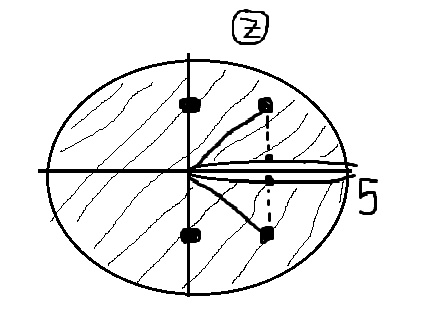
\includegraphics[width=0.4\textwidth]{49-50D.png}
\end{wrapfigure}
\oar\bigskip
\textbf{Пример.} 
\par\bigskip

$D = B(0; 5)$ с разрезом 

$\rho_D(-i, i) = 2, $

$\rho_D(1-i, 1+i) = 2 \sqrt{2}$.

$a = 1$ --- точка на верхнем береге разреза;

$b = 1$ --- точка на нижнем береге разреза.

$\rho_D(a, b) = 2,$ 

$\rho_D(a, 0) = 1,$

$\rho_D(a, 1-i) = 1 + sqrt(2)$
\par\bigskip
Пусть $D$ --- ограниченная область, граница которой $\partial D$ состоит из конечного числа замкнутых кривых $\gamma_1, \gamma_2, ..., \gamma_n$. Пусть функция $f$ определена на $D \cup \partial D$.
\par\bigskip
Функцию $f(z)$ будем называть \textbf{непрерывной в области $D$ вплоть до границы $\partial D$}, если для каждой точки $a \in D \cup \partial D$ имеет место равенство $f(a) = \lim\limits_{\rho_D(z,a)\rightarrow 0}f(z)$.
\par\bigskip
Если $a$ --- внутренняя точка, или $a$ не является точкой самопересечения граничной кривой, то $\lim\limits_{\rho_D(z,a)\rightarrow 0}f(z) = \lim\limits_{z\rightarrow a}f(z)$, т.е. понятие непрерывности в такой точки обычное.

Таким образом, если граница $\partial D$ области $D$ состоит из простых кривых (замкнутых), то непрерывность $f$ вплоть до границы равносильна непрерывности $f$ в $\overline{D} = D \cup \partial D$. Но если $\partial D$ не является простой, то из непрерывности $f$ вплоть до границы не следует непрерывность $f$ на $\overline{D}$.

\textbf{Пример.}\quad $f(z) = \sqrt{z} = z^{\frac{1}{2}}e^{\frac{i\phi}{2}}$, где $z = \rho \cdot e^{i\phi},\quad 0 < \phi < 2\pi$.
\par\bigskip
Доопределим $f$ в каждой граничной точке $a$ области как на рисунке вначале параграфа по формуле: $f(a) = \lim\limits_{\rho_D(z, a) \rightarrow 0}$. Эта функция непрерывна в $D$ вплоть до границы. В частности, если $z = x > 0$ на верхнем береге разреза, то $$\lim\limits_{\rho_D(z,a)\rightarrow 0}f(z) = \lim\limits_{z\rightarrow x, Im(z) > 0}f(z) = f(x + 0\cdot i) = \sqrt{x}$$

На нижнем береге разреза $z = x > 0$, получаем $$\lim\limits_{\rho_D(z,a)\rightarrow 0}f(z) = \lim\limits_{z\rightarrow x, Im(z) < 0}f(z) = f(x - 0\cdot i) = -\sqrt{x}$$

Отсюда следует, что $f(z)$ не является непрерывной в $\overline{D}$.



\section{Интегральная теорема Коши}
Продолжим разговор об интегралах. Речь пойдёт об интегральной теореме Коши --- одном из наиболее важных результатов в теории ФХП.
\par\bigskip

\textbf{Теорема.} \quad
\textit{Пусть f однозначна и дифференцируема в конечной односвязной области D и пусть её производная f'(z) непрерывна в D. Тогда интеграл от f(z) по любой замкнутой кривой l, целиком лежащей в D, равен нулю:}
$$\int\limits_l f(z)\,dz=0 $$\\
\blacklozenge \hspace{4 mm}
\text{Воспользуемся формулой} \par
$$\int\limits_l f(z)\,dz = \int\limits_l u\,dx - v\,dy + i\int\limits_lv\,dx+u\,dy$$

Так как $f$ обладает непрерывной производной в области $D$, то все частные производные первого порядка функции $u(x,y),\ v(x,y)$ --- непрерывны в области $D$ и в этой области удовлетворяют условиям Коши--Римана
$$\frac{\partial u}{\partial x} = \frac{\partial v}{\partial y}\quad ,\quad \frac{\partial u}{\partial y} = - \frac{\partial v}{\partial x}$$

Но эти условия для КРИ-2 представляют собой условия независимости от пути интегрирования, и, значит, КРИ равны 0.

Поэтому и $\int\limits_l f(z)\,dz=0$. \quad
\blacksquare
\par\bigskip

Иногда эту теорему формулирую в следующем виде:
\par\bigskip
\textit{Если f(z) непрерывно дифференцируема в односвязной конечной области D, ограниченной кусочно-гладким контуром $\partial D$ и непрерывна в $\overline D = D \cup \partial D$ (или вплоть до границы), то $\int\limits_{\partial D} f(z)\, dz = 0$.}
\par\bigskip

Отмечу также, что теорема верна и в случае, если f --- дифференцируема (непрерывность не обязательна!). Есть доказательство Гурса (см., например, Сидоров и др.)

Теорему можно распространить и на неодносвязную область.
\par\bigskip

\textbf{Теорема.} \quad
\textit{Пусть граница $\partial D$ многосвязной области D состоит из замкнутой кусочно-гладкой кривой $l_0$ и попарно непересекающихся замкнутых кусочно-гладких кривых $l_1,\ l_2, \ldots ,\ l_n$, расположенных внутри $l_0$ и пусть функция f(z) дифференцируема в области D и непрерывна в $\overline D$. Тогда}
$$\int\limits_{\partial D} f(z)\,dz=0\ ,$$
\textit{где каждый из контуров обходится в положительном направлении, то есть так, что область остаётся слева.}\\

\begin{wrapfigure}[7]{l}{0.3\linewidth} 
\vspace{-6ex}
    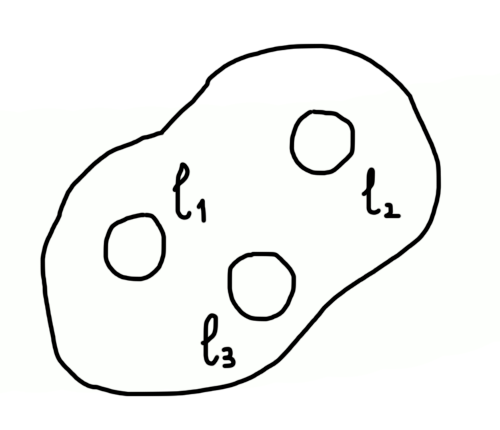
\includegraphics[width=5 cm]{koshi.png}
\end{wrapfigure}

$\blacklozenge$ \hspace{1 mm}
Для доказательства проводим разрезы так, чтобы получившаяся область была связной по теореме Коши для односвязных областей.
$$\int\limits_\gamma f(z)\,dz = 0 $$
Интегралы по разрезам уничтожаются. \quad \blacksquare
\par\bigskip

\textbf{Следствие 1.} \quad
В условиях теоремы Коши $\int\limits_{l_1} f(z)\,dz = \int\limits_{l_2} f(z)\,dz$, если $l_1 \subset D,\ l_2 \subset D$ и имеют одни и те же концы.
\par\bigskip

\textbf{Следствие 2.} \quad
$\int\limits_{\gamma_1}f(z)\,dz = \int\limits_{\gamma_2}f(z)\,dz$, если $\gamma_1$ и $\gamma_2$ замкнуты, $\gamma_1 \subset D,\ \gamma_2 \subset D$ и $\gamma_1$ и $\gamma_2$ охватывают одни и те же лакуны.


\section{Неопределённый интеграл}
Пусть $f(z)$ дифференцируема в односвязной области $D$. Обозначим
$$\Phi(z) := \int\limits_{z_0}^z f(\xi)\,d\xi,$$
где $z_0$ --- фиксированная точка области $D$, $z$ --- произвольная точка области $D$.
\par\bigskip Функция $\Phi$ является однозначной функцией z, поскольку в силу теоремы Коши \\(см. Следствие 1) интеграл $\int\limits_{z_0}^{z} f(\xi)\,d\xi$ не зависит от формы пути интегрирования. Тем самым оправдана форма записи интеграла.
\par\bigskip

\textbf{Теорема.} \quad \textit{Пусть функция f определена и непрерывна в конечной односвязной области D и интеграл от этой функции по любому замкнутому контуру, лежащему в D, равен нулю. Тогда функция $\Phi(z)$ дифференцируема в области D и $\Phi'(z)=f(z)$, то есть}
$$\left( \int\limits_{z_0}^z f(\xi)d\xi \right) ' = f(z)$$

\blacklozenge \quad 
Функция $\Phi$ однозначна в $D$, поскольку интеграл по любому замкнутому контуру равен нулю. Составим отношение:
\[\frac{\Delta \Phi}{\Delta z} = \frac{\Phi(z + \Delta z)-\Phi(z)}{\Delta z} = \frac{1}{\Delta z} \left( \int\limits_{z_0}^{z+\Delta z}f(\xi)\,d\xi - \int\limits_{z_0}^z f(\xi)\,d\xi \right) = \frac{1}{\Delta z} \int\limits_{z_0}^{z+\Delta z}f(\xi)\,d\xi,\]
так как интеграл не зависит от формы пути интегрирования. Здесь предполагается, что $z+\Delta z \in D.$

Возьмём в качестве пути интегрирования отрезок, принадлежащий $D$. Так как $D$ --- область, то все точки внутренние и $\exists U(z) \in D$. Считаем, что $z+\Delta z \in U(z)$.

\par\bigskip Оценим теперь следующую величину
\[\left | \frac{\Delta \Phi}{\Delta z} - f(z) \right | = 
\left | \frac{1}{\Delta z}\int\limits_z^{z+\Delta z}f(\xi)\,d\xi - \frac{1}{\Delta z}\int\limits_z^{z+\Delta z}f(z)\,d\xi \right | = 
\frac{1}{|\Delta z|}\left | \int\limits_z^{z+\Delta z}(f(\xi) - f(z))d\xi \right | \leqslant\]
\[\leqslant \frac{1}{|\Delta z|}\int\limits_z^{z+\Delta z}|f(\xi) - f(z)| d\xi \leqslant 
\otimes\]
Так как $f$ непрерывна в $D$, в частности в точке $z$, то $\forall \epsilon > 0,\ 
\exists \delta (\epsilon)>0,\ 
\forall \xi,\ 
|\xi - z| \leqslant \delta \Rightarrow
|f(z) - f(\xi)| \leqslant \epsilon$

$$\otimes \leqslant 
\frac{1}{|\Delta z|} \int\limits_z^{z+ \Delta z} \epsilon \xi d\xi =
\frac{\epsilon}{|\Delta z|} \cdot |\Delta z| = 
\epsilon$$

Причём, это неравенство выполняется для 
$\forall \xi \in [z,\ z+\Delta z]$, если 
$|\Delta z| \leqslant \delta (\epsilon)$.

Итак, существует 
$\lim\limits_{\Delta z \to 0}\frac{\Delta \Phi}{\Delta z} = f(z)$, то есть 
$\Phi '(z) = f(z)$.
\blacksquare

Доказанная теорема позволяет ввести понятие первообразной и неопределенного интеграла ФКП.
\par\bigskip

Пусть $f$ определена в области $D$ и $F$ --- дифференцируема в $D$. Если $F'(z) = f(z)$, для всех $z \in D$, то $F(z)$ называют \textbf{первообразной функции $f$ в области $D$}.
\par\bigskip
Совокупность всех первообразных в $D$ называют \textbf{неопределённым интегралом от $f$}.
\par\bigskip

Из доказанной теоремы вытекает, что, если $f$ непрерывна в односвязной области $D$, и интеграл по любому замкнутому контуру из $D$ равен нулю, то $f$ обладает первообразной $\Phi(z) = \int\limits_{z_0}^z f(\xi)\,d\xi$.
\par
В частности, если $f$ дифференцируема в конечной односвязной области $D$, то она имеет в этой области первообразную. Действительно, в этом случае $f$ удовлетворяет условиям предыдущей теоремы, поскольку, по теореме Коши, интеграл по любому замкнутому контуру равен нулю, и, поэтому, $\Phi(z) = \int\limits_{z_0}^z f(\xi)\,d\xi$ является первообразной для $f$. Отметим, что, если $\Phi(z)$ --- первообразная, то и всякая функция вида $\Phi(z) + C$ также будет первообразной ($C$ --- произвольное комплексное число). Верно и обратное.
\par\bigskip

\textbf{Теорема.}
\quad \textit{Совокупность всех первообразных функции f(z) в области D определяется формулой F(z)+C, где F --- какая-нибудь первообразная функции f, а C --- произвольная комплексная постоянная.} \\
\blacklozenge \hspace{4 mm}
Пусть $F_1(z)$ и $F_2(z)$ --- две первообразные функции $f$ в области $D$. Тогда функция $F(z) = F_1(z) - F_2(z) = u + iv$ есть постоянная в области $D$. Действительно, по условию $F'(z) = F_1'(z) - F_2'(z) = f(z) - f(z) = 0$ для всех $z \in D$. Отсюда следует, что
\[F'(z) = 
\frac{\partial u}{\partial x}+i\frac{\partial v}{\partial x}=
\frac{\partial v}{\partial y}-i\frac{\partial u}{\partial y}= 0 \quad \Rightarrow \quad
\frac{\partial u}{\partial x} = 
\frac{\partial u}{\partial y} = 
\frac{\partial v}{\partial x} =
\frac{\partial v}{\partial y} =
0 \Rightarrow\]
\[\Rightarrow u = C_1,\ v = C_2 \quad \Rightarrow \quad
F(z) = C_1 + iC_2 = C\] \blacksquare

\bigskip
Техника вычисления неопределённого интеграла такая же, как и для действительных функций. 

Например:
$$\int e^z\,dz = e^z + C,\qquad \int z^n\,dz = \frac{z^{n+1}}{n+1}\quad (n \ne -1)$$
\par\bigskip

Имеет место формула Ньютона--Лейбница
$$\int\limits_{z_0}^{z_1}f(\xi)\,d\xi = \Phi(z_1)-\Phi(z_0)$$

\begin{Proof}
\[\Phi(z) = \int\limits_{z_0}^{z}f(\xi)\,d\xi + C \quad \Rightarrow \quad \Phi(z_0) = C,\]
\[\Phi(z_1) =  \int\limits_{z_0}^{z_1}f(\xi)\,d\xi + C = \int\limits_{z_0}^{z_1}f(\xi)\,d\xi + \Phi(z_0) \quad \Rightarrow \quad \int\limits_{z_0}^{z_1}f(\xi)\,d\xi = \Phi(z_1) - \Phi(z_0)\]
\end{Proof}

Справедлива формула интегрирования по частям.

Если область $D$ неодносвязна, то всё усложняется. Функция $\Phi(z)$ может быть уже неоднозначной, интеграл зависит от пути интегрирования.

Например:
$$\int\limits_1^z\frac{d\xi}{\xi} = \ln z + 2k\pi i = Ln\,z$$

Этот интеграл в области $Re\,z > 0$ не зависит от пути интегрирования, так как там функция дифференцируема и область односвязна. Если же в качестве контура интегрирования взять окружность $|z| = 1$, то $\int\limits_{|z|=1}\frac{dz}{z} = 2\pi i$. Получаем, что интеграл не равен нулю по замкнутому контуру. Всё потому, что функция разрывна в точке $z = 0$ (в области, ограниченной окружностью). Но мы можем считать её дифференцируемой в двусвязной области, получающейся, если у круга $|z| \leqslant 1$ выбросить точку $z = 0$.
\par\bigskip

\textbf{Пример 1.} \quad
$I = \int\limits_0^i z\sin z\,dz$.

Подынтегральная функция однозначна и дифференцируема во всей плоскости, значит интеграл не зависит от пути интегрирования. Можно интегрировать по частям:
\[\begin{matrix} 
u = z && dv = \sin z\:dz \\ du = dz && v = -\cos z
\end{matrix} \quad \Rightarrow \quad 
I = \bigl. -z\cos z \bigr|_0^i + \bigl. \sin z \bigr|_0^i = -i\cos i + 0 + \sin i - 0 = \]
\[= -i(\cos i + i\sin i) = -ie^{i\cdot i} = -ie^{-1};\]
\par\bigskip

\textbf{Пример 2.} \quad
$\int\limits_{-1}^1 \bar z\,dz$ --- по верхней полуокружности $|z| = 1$. Функция не дифференцируема, не зависит от пути интегрирования (вообще говоря, сводим к ОИ:
$$z = e^{i\phi},\ \bar z = e^{-i\phi},\ dz = ie^{i\phi}d\phi \quad \Rightarrow \quad
\int\limits_{-1}^1 \bar z\,dz = \int\limits_\pi^0 e^{-i\phi}\cdot ie^{i\phi}\,d\phi = -\pi i.$$










\section{Интегральная формула Коши}

Доказанная теорема Коши позволяет установить ряд важных следствий, в частности позволяет установить определённую связь между значениями дифференцируемой функций во внутренних точках области её дифференцируемости и граничными значениями этой функции. А именно, имеет место следующая теорема.

\par\bigskip

\textbf{Теорема.} \quad
\textit{Пусть функция $f$ дифференцируема в односвязаной области $D$ и $L$ - простой замкнутый контур целиком лежащий в $D$, $z_0$ - точка из $D$, лежащая внутри контура $L$. Тогда:}
\[
    f(z_0) = \frac{1}{2\pi i}\oint\limits_{L}\frac{f(z)}{z-z_0}dz
\]
\textit{где $L$ обходится в положительном направлении.}

Эта формула называется \textbf{интегральной формулой Коши}, а интеграл - \textbf{интегралом Коши}\\
\blacklozenge \hspace{4 mm}
Построим $\gamma_\rho ::= S(z_0, \rho)$ так, $\gamma_\rho$ принадлежала области , ограниченной контуром $L$.
\begin{center}
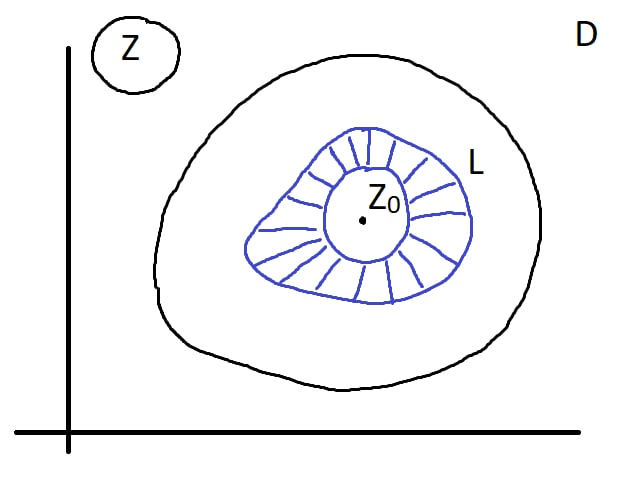
\includegraphics[width=0.5\linewidth]{complex1}
    
\end{center}

Тогда, на основании теоремы Коши для многосвязных областей, получим:


\[
    \oint\limits_{L}\frac{f(z)}{z-z_0}dz = \oint\limits_{\gamma_\rho}\frac{f(z)}{z-z_0}dz,
\]
\par или
\[
    \frac{1}{2\pi i}\oint\limits_{L}\frac{f(z)}{z-z_0}dz = \frac{1}{2\pi i}\oint\limits_{\gamma_\rho}\frac{f(z)}{z-z_0}dz
\]

Рассмотрим модуль разности:
\[
    |\frac{1}{2\pi i}\oint\limits_{\gamma_\rho}\frac{f(z)}{z-z_0}dz - f(z_0)| = |\frac{1}{2\pi i}\oint\limits_{\gamma_\rho}\frac{f(z)}{z-z_0}dz - \frac{1}{2\pi i}\oint\limits_{\gamma_\rho}\frac{f(z_0)}{z-z_0}dz| =
\]
\[
    = \frac{1}{2\pi}|\oint\limits_{\gamma_\rho}\frac{f(z)-f(z_0)}{z-z_0}dz| \leq 
    \frac{1}{2\pi}\oint\limits_{\gamma_\rho}\frac{|f(z)-f(z_0)|}{|z-z_0|}dz
\]

Так как $f$ непрерывна в точке $z_0$:
\[
    \forall \epsilon > 0, \exists \delta_\epsilon > 0, \forall \rho \leq \delta_\epsilon \rightarrow |f(z)-f(z_0)| \leq \epsilon
\]

Тогда имеем:
\[
     \frac{1}{2\pi}\oint\limits_{\gamma_\rho}\frac{|f(z)-f(z_0)|}{|z-z_0|}dz \leq  =
    \frac{1}{2\pi}\oint\limits_{\gamma_\rho}\frac{\epsilon}{|z-z_0|}dz < \frac{\epsilon}{2\pi\rho}\oint\limits_{\gamma_\rho}dz = \frac{\epsilon}{2\pi \rho} \cdot 2\pi\rho = \epsilon
\]

Так как разность между двумя величинами не зависит от $\rho$ за счёт выбора $\rho$ может быть сделана сколь угодно малой, что это разность есть $0$, то есть:
 \[
    \frac{1}{2\pi i}\oint\limits_{L}\frac{f(z)}{z-z_0}dz = \frac{1}{2\pi i}\oint\limits_{\gamma_\rho}\frac{f(z)}{z-z_0}dz = f(z_0)
 \]
\blacksquare
 
\section{Замечания и следствия формулы Коши}
\begin{enumerate}
  \item Теорема может быть сформулирована в следующем виде:
  
  \textit{Если $f$ дифференцируема в односвязной области $D$ и непрерывна в $\overline{D}$}, то
  \[
    \frac{1}{2\pi i} \oint\limits_{\delta D}\frac{f(\zeta)}{\zeta - z}d\zeta = f(z)
  \]
  
  Согласно этой формуле, на интеграл Коши можно смотреть как на интеграл зависящий от параметра.
  
  \item Теорема остается справедливой и для многосвязной области $D$. При этом, при выводе формулы в качестве $\gamma_\rho$ следует взять окружность, которая может быть стянута в точку $z_0$, всё время оставаясь в $D$.
  \[
    \frac{1}{2\pi i} \oint\limits_{\delta D}\frac{f(z)}{z - z_0}dz = f(z_0)
  \]
  
  \item В условиях теоремы
  \[
    \frac{1}{2\pi i} \oint\limits_{\delta D}\frac{f(z)}{z - z_0}dz = 
    \begin{cases}
    f(z_0), z_0 \in D\\
    0, z_0 \notin \overline{D}\\
    \nexists, z_0 \in \delta D
    \end{cases}
  \]
  
  \item
  \textbf{Теорема о среднем.} \quad
  \textit{Пусть $f$ дифференцируема в шаре $B(z_0; R)$ и непрерывна в $\overline{B}(z_0; R)$. Тогда значение этой функции в центре круга равно среднему арифметическому её значений на окружности $\gamma_R = S(z_0; R)=\delta B(z_0; R)$. То есть:
  \[
    f(z_0) = \frac{1}{2\pi R}\oint\limits_{\gamma_R}f(z)ds = \frac{1}{2\pi}\int\limits_{0}^{2\pi}f(z_0 + R e^{i\phi})d\phi
  \]}
  \begin{Proof}
  \[
    f(z_0) = \frac{1}{2\pi i}\oint\limits_{\gamma_R}\frac{f(z)}{z-z_0}dz = [z=z_0 + R e^{i\phi}] = \frac{1}{2\pi i}\int\limits_{0}^{2\pi}\frac{f(z_0+R e^{i\phi})}{R e^{i\phi}}\cdot R i e^{e\phi}d\phi = 
  \]
  \[
    \frac{1}{2\pi}\int\limits_{0}^{2\pi}f(z_0 + R e^{i\phi}d\phi = [\text{Для круга имеем:} Rd\phi = ds] = \frac{1}{2\pi R}\int\limits_{\gamma_R}f(z)ds
  \]
  \end{Proof}
  
  Эту теорему ещё называют и \textbf{теоремой Гаусса.}
  \end{enumerate}
  
  Как следствие, получаем теорему о среднем для гармонической функции:
  
  \textbf{Теорема (о среднем для гармонической функции).} \quad \textit{Пусть $u(x_0, y_0)$ - гармоническая в кругу $B(z_0; R)$ и непрерывна в $\overline{B}(z_0; R)$. Тогда:
  \[
    u(x_0, y_0) = \frac{1}{2\pi}\int\limits_{0}^{2\pi}u(x_0 + Rcos\phi, y_0 + Rsin\phi)d\phi
  \]
  } \\
  \blacklozenge \hspace{4 mm}
    Построим $f(z)$ так, чтобы $u(x, y)=Re f(z)$ и $f$ - дифференцируема в $B(z_0; R)$. Тогда:
    \[
        f(z_0) = \frac{1}{2\pi}\int\limits_{0}^{2\pi}f(z_0 + \rho e^{i\phi})d\phi, \; \text{где } 0 < \rho < R
    \]
    
    Приравняем действительные части:
    \[
        u(x_0, y_0) = \frac{1}{2\pi} \int\limits_{0}^{2\pi}u(x_0+\rho cos\phi, y_0 + Rsin\phi)d\phi
    \]
    
    Перейдем к приделу где $\rho \rightarrow R$ и получим требуемое.
  \blacksquare
  
  
  
  
  
  
  
  
  
\section{Принцип максимума модуля дифференцируемой ФКП}
\par\bigskip
\textbf{Теорема.} \textit{\quad Пусть $f$ дифференцируема в области $D$ и непрерывна в $\overline{D}$.Тогда или $|f(z|\equiv const$ в области $D$, или максимальное значение $|f(z)|$ достигается только на границе $\partial D$ области D.} \\
\bigskip
$\blacklozenge$ \hspace{1 mm} $f(z)=u(x,y)+iv(x,y)$
\par
Поэтому $|f(z)|=\sqrt{u^2(x,y)+v^2(x,y)}$ непрерывна в $\overline{D}$ и на основании теоремы Вейерштрасса о достижении точных границ она достигает максимума в $\overline{D}$. Обозначим через $z_0$ точку максимума:
$$|f(z_0)|= \max_{z \in \overline{D}} |f(z)|$$
\par Предположим, что  $z_0\in D$(т.е. $z_0$ внутренняя точка области D, $z_0\not\in \partial D$).


\begin{wrapfigure}[8]{l}{0.3\linewidth} 
    \vspace{-25pt}
    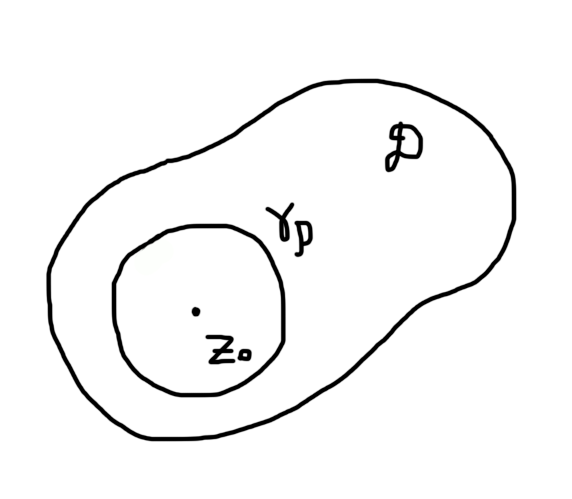
\includegraphics[width=0.3\textwidth]{max mod FKP/1maxModFKP.png}
\end{wrapfigure}

\par\bigskip Построим окружность $\gamma_g=S(z_0, g)$ так, чтобы $\overline{\gamma_g}\in D$. Тогда по теореме о среднем $$f(z_0)=\frac1{2\pi g}\int_{\gamma_g}f(z)ds$$

Отсюда следует:
 \par\bigskip
$|f(z_0)|\leqslant \frac1{2\pi g}\int_{\gamma_g}|f(z)|ds \leqslant \frac1{2\pi g}\max_{\gamma_g} |f(z)| *2\pi g=\max_{\gamma} |f(z)|$\quad\quad(1)\\
 \par\bigskip
 C другой стороны, согласно выбору точки $z_0: |f(z_0)|\geqslant |f(z)|\quad \forall z\in \overline{D}$
 \par\bigskip
 Отсюда следует, что: $\max_{\gamma_g} |f(z)|\le |f(z_0)|$\quad\quad (2)
 \par\bigskip
 Из (1) и (2) следует, что $\max_{\gamma_g} |f(z)|= |f(z_0)|$, 
 т.е. $\exists z^* \in \gamma_g , \quad |f(z^*)|=|f(z_0)|$
 \par\bigskip
 Покажем теперь, что $\forall z \in \gamma_g |f(z)|=|f(z_0)|$
 
 \begin{wrapfigure}[10]{l}{0.3\linewidth} 
    \vspace{-15pt}
    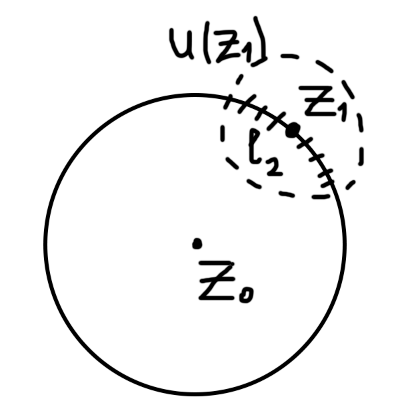
\includegraphics[width=0.2\textwidth]{max mod FKP/2maxModFKP.png}
\end{wrapfigure}
 \par\bigskip
 Предположив, что в какой-то точке $z_1 \in \gamma_g$ выполняется $|f(z_1)|<|f(z_0)|$ , мы найдем такую окрестность $U(z_1)$ точки $z_1$, что в силу непрерывности функции f(z):
 
 $$\forall z \in U(z_1) \cap \gamma_g \quad|f(z)|<|f(z_0)$$
 
 А тогда:\par$$\frac1{2\pi g}\int_{\gamma_g}|f(z)|ds=\frac1{2\pi g}\int_{l_1}|f(z)|ds+\frac1{2\pi g}\int_{l_2}|f(z)|ds< \frac1{2\pi g}|f(z_0)|*length\  l_1+$$
 
$$ +\frac1{2\pi g}|f(z_0)|*length\  l_2=|f(z_0)|$$
\par\bigskip
Таким образом \quad 
\begin{center}
    $|f(z_0)|>\frac1{2\pi g} \int_{\gamma_g}|f(z)|ds$
\end{center}
\par\bigskip
На основании же теоремы о среднем вытекает, что
\begin{center}
    $|f(z_0)|\leqslant \frac1{2\pi g} \int_{\gamma_g}|f(z)|ds$
\end{center}
\par\bigskip
Получаем противоречие. 
\par\bigskip Значит, $\forall z \in \gamma_g |f(z)|=|f(z_0)|$
\par\bigskip
Отсюда вытекает, что на окружности $\gamma_g$ функция |f(z)| имеет постоянное значение, равное своему максимальному значению в $\overline{D}$. Аналогичным образом рассуждая для $\gamma_{g_1}$, где $g_1<g$, приходим к выводу,
что $|f(z)|=|f(z_0)| \quad \forall z \in \overline{B}(z_0,g)$
\par\bigskip
Покажем теперь, что и в любой точке $\forall z' \in D \quad|f(z')|=|f(z_0)|$
С этой целью соединим точки $z_0$ и $z'$ спрямляемой кривой $l$, целиком лежащей в D.

\begin{wrapfigure}[5]{l}{0.2\linewidth} 
    \vspace{-15pt}
    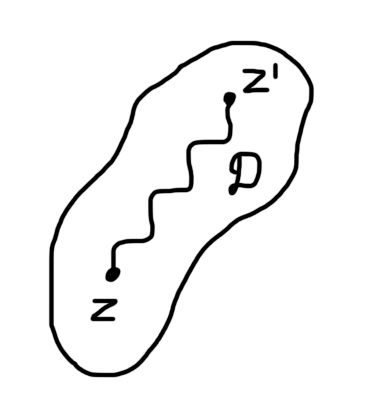
\includegraphics[width=0.2\textwidth]{max mod FKP/3maxModFKP.png}
\end{wrapfigure}
 \par\bigskip

\par\bigskip
$d::=g(l,\partial D)=0$
\par\bigskip
Разобьем $l$ точками $z_0,z_1,..., z_n=z'$ на дуги $l_1,l_2,..., l_n$ таким образом, чтобы длина $l_k$ была меньше $\frac{d}{2}$.

Построим систему кругов $B(z_k, \frac{d}{2})$.
Тогда $\bigcup\limits_{k=0}^n B(z_k, \frac{d}{2}) \subset D,\par l \in \bigcup\limits_{k=0}^n B(z_k, \frac{d}{2}) $

\par\bigskip
Действительно, если $z\in l_k$, то $|z-z_k|\leqslant length\quad l_k < \frac{d}{2}$,\quad т.е. дуга  $l_k \in B(z_k,\frac{d}{2})$ и $\gamma=\bigcup\limits_{k=1}^n \gamma_k \subset \bigcup\limits_{k=0}^n B(z_k, \frac{d}{2}) $

Так как $z_1 \in  B(z_0, \frac{d}{2}) \subset B(z_0, g) $ и $|f(z_1)|=|f(z_0)|$, то в круге $B(z_1, \frac{d}{2})$ \quad$|f(z)|=|f(z_0)|$ и т.д. пока не придем к точке $z'$ и $|f(z')|=|f(z_0)|$
\par\bigskip
Значит, из предположения, что $|f(z)|$ достигает максимума во внутренней точке области D следует, что $|f(z)|=const$. А поскольку известно, что $|f(z)|\not=const $,то получаем противоречие. Следовательно, $|f(z)|$ не может достигать своего максимума во внутренней точке области D. Но так как максимум существует, то он обязательно лежит на $\partial D.\quad \blacksquare$
\quad\bigskip

\textbf{Замечания:}
\begin{enumerate}
    \item \textit{ Имеет место и принцип минимума модуля: если f дифференцируема в D, непрерывна в $\overline{D}$ и $f(z)\not= 0$ ни в одной точке области D, то минимум $|f(z)|$ достигается на $\partial D$.}\\
    $\blacklozenge$\quad  Для доказательства достаточно применить принцип максимума модуля к функции $\frac1{|f(z)|}.\quad \blacksquare$

    \item \textit{Аналогичная теорема имеет место и для гармонических функций: гармоническая в области D функция, не являющаяся постоянной, принимает свои максимальные  и минимальные значения на границе области D.}
    
    \item \textit{ Если f дифференцируема и $|f|=C \quad \forall z\in D$, то $|f(z)|=const$ } \\
    $\blacklozenge$ \quad Функция $ln f(z)$ имеет постоянную действительную часть 
    $ln |f(z)|$. На основании условий Коши-Римана дифференцируемая функция с постоянной действительной частью постоянна, а значит и $f(z)$ постоянна. \quad $\blacksquare$
\end{enumerate}








\section{Ряды с комплексными членами(числовые, функциональные, степенные)}
\subsection{Числовые ряды}


Ряд  $\sum z_k $ называется \textbf{сходящимся}, если сходится последовательность его частных сумм: $S_n= \sum\limits_{k=1}^n z_k$
\par\bigskip

При этом $S= \lim\limits_{n \to \infty} S_n$ называют \textbf{суммой ряда}.
\par\bigskip
Ряд $\sum z_k $ называется \textbf{абсолютно сходящимся}, если сходится ряд $\sum |z_k| $. Если же $\sum z_k $ сходится, а  $\sum |z_k| $ расходится, то говорят, что $\sum z_k $ сходится \textbf{неабсолютно(условно)}.
\par\bigskip
Из свойств сходящихся последовательностей вытекают следующие свойства рядов:
\begin{enumerate}
    \item \textit{Для сходимости ряда $\sum z_k $, где $z=x+iy$, необходима и достаточна сходимость рядов $\sum x_k $ и $\sum y_k $. При этом:
    $\sum z_k =\sum x_k+ i\sum y_k $}
    \item  \textit{Из сходимости ряда $\sum z_k $ следует сходимость ряда $\sum az_k $, где $a\in \mathbb{C}$, и при этом выполняется равенство:
    $$\sum az_k=a\sum z_k$$}
    \item \textit{Если сходятся ряды $\sum z_k$ и $\sum \xi_k$, то сходится и ряд $\sum (z_k+\xi_k)$, и при этом $\sum z_k + \sum \xi_k=\sum (z_k+\xi_k)$}
    \item \textit{Критерий Коши сходимости}:
    $$\forall \epsilon>0\quad \exists \nu(\epsilon)>0 \quad \forall n,m \geqslant \nu(\epsilon)\quad \left| \sum\limits_{k=n}^{m+n} z_k \right|\leqslant\epsilon$$
    \item \textit{Если $\sigma=\sum \xi_k$, $s=\sum z_k$, и если хотя бы один из рядов сходится абсолютно, то и их произведение сходится, при этом
$\sum z_k \sum \xi_k=\sum c_k$, где $c_k=\sum\limits_{n=1}^k z_n\xi_{k-n+1}$ и $\sum c_k=\sigma s$}
\end{enumerate}



\section{Ряды функций}  

Изучаются по той же схеме, что и ряды с действительными членами.
Вспомним основные определения для действительных рядов:

\begin{enumerate}
    \item Последовательность функций $(f_n(z))$ называется \textbf{сходящейся} к функции $f(z)$ на множестве D, если $$\forall z\in D\quad \lim_{n \to \infty} f_n(z)=f(z)$$
    \item Последовательность функций $(f_n(z))$ называется \textbf{равномерно сходящейся} к функции $f(z)$ на множестве D, если
    $$\forall \epsilon>0 \quad\exists \nu(\epsilon) \quad \forall n\geqslant \nu(\epsilon) \quad \forall z \in D \quad |f_n(z)-f(z)|\leqslant \epsilon$$
    \item  Ряд $\sum f_k(z) $ \textbf{сходится(поточечно)} на множестве D, если он сходится как числовой ряд в каждой точке D.
    \item Ряд $\sum f_k(z) $ \textbf{сходится равномерно} на множестве D, если последовательность его частных сумм сходится равномерно D.
\end{enumerate}

\par\bigskip
Для рядов функций справедливы следующие утверждения, которые доказываются так же, как это было в действительных рядах:
\quad\bigskip
\begin{enumerate}
    \item \textbf{Критерий Коши} \par
    Для того, чтобы ряд $\sum f_k(z) $ сходился равномерно на множестве D, необходимо и достаточно, чтобы:
    $$\forall \epsilon>0 \quad\exists \nu(\epsilon) \quad \forall n\geqslant \nu(\epsilon) \quad \forall p\geqslant 0 \quad \forall z \in D \quad \left| \sum\limits_{k=n}^{n+p} f_k(z)\right|\leqslant  \epsilon$$
    \item \textbf{Признак Вейерштрасса} \par
    Если для ряда $\sum f_k(z) $ существует сходящаяся числовая
    мажоранта, то он сходится равномерно на D:
    $\forall k \quad \forall z \in D \quad|f_k(z)|\leqslant c_k \quad ,  \sum c_k \longrightarrow$, то $\sum f_k(z) \rightrightarrows$
    
    \item \textbf{Непрерывность суммы и почленное интегрирование}\par
    Если  $ f_k(z) $ непрерывны в области D, а ряд  $\sum f_k(z) $ сходится равномерно в D и f(z) есть его сумма, то:
    \begin{enumerate}
        \item f(z) непрерывна в D;
        \item ряд можно интегрировать почленно вдоль любой кусочно-гладкой кривой l из D, т.е.
        $\int\limits_l f(z)dz= \sum\limits_{k=1}^\infty \int\limits_l f_k(z)dz$
    \end{enumerate}
\end{enumerate}


\section{Степенные ряды}  

\textbf{Степенной ряд} -- это ряд вида:

$$\sum\limits_{k=0}^\infty c_k (z-z_0)^k,$$ где $c_k, z_0 \in \mathbb{C}$, z-комплексная переменная.

\par\bigskip
\textbf{Множество сходимости степенного ряда} -- множество точек из $\mathbb{C}$, для которых ряд сходится. Для комплексных степенных рядов справедливы все утверждения, сформулированные ранее для действительных рядов, лишь слово "интервал" следует заменить на "открытый круг". Каждый степенной ряд обладает \textbf{радиусом сходимости} R таким, что в открытом круге $B(z_0;R)$ степенной ряд сходится, а вне круга $\overline{B}(z_0;R)$ расходится. Этот круг в отдельных случаях может вырождаться в точку или быть всей комплексной плоскостью. 
\par\bigskip
Находится радиус сходимости по формуле Коши-Адамара:
$$R=\frac1{\varlimsup\limits_{n \to \infty} \sqrt[n]{|c_n|}}$$
\par или $R=\lim\limits_{n \to \infty} \left| \frac{c_n}{c_{n+1}} \right|$, если он существует

\par\bigskip
В круге $B(z_0;R)$ степенной ряд сходится абсолютно и равномерно, т.е. он сходится равномерно в любой замкнутой области $\overline{D} \subset B(z_0;R) $

Сумма степенного ряда является функцией, непрерывной в круге сходимости.
$$f(z)=\sum\limits_{k=0}^\infty c_k(z-z_0)^k$$

Коэффициенты $c_k$ степенного ряда связаны с функцией f следующим образом:
$$c_k=\frac{f^{(k)}(z_0)}{k!},$$ т.е. степенной ряд является рядом Тейлора своей суммы.
\par\bigskip
Разложение функции в степенной ряд единственно. Степенной ряд можно дифференцировать(и почленно интегрировать) в круге сходимости нужное число раз.

\par\bigskip
\textbf{Примеры:} $\sum z^n, \sum \frac{z^n}{n}, \sum \frac{z^n}{n^2}$

\begin{enumerate}
    \item $\frac1{(1-z)^2}=\left( \frac1{1-z}\right)'=(1+z+z^2+...+)'=1'+z'+(z^2)'+... =1+2z+3z^2+4z^3+...=\sum\limits_{k=0}^\infty (k+1)z^k$
    \item $ln(1+z)=\int\limits_0^z \frac{dz}{1+z}=\int\limits_0^z (1-z+z^2-z^3+...)dz=\int\limits_0^z dz-\int\limits_0^z zdz+\int\limits_0^z z^2dz-...=z-\frac{z^2}{2}+\frac{z^3}{3}-...=\sum\limits_{k=1}^\infty (-1)^{k+1} \frac{z^k}{k}$
\end{enumerate}



\par\bigskip
\section{Регулярные функции}

\subsection{Связь регулярных и дифференцируемых функций (критерий регулярности функции)}
Пусть функция $f$ определена в окрестности точки $z \ne \infty$ и представима в этой окрестности степенным рядом $\sum\limits_{k=0}^\infty c_k(z - z_0)^k = f(z)$, сходящимся в некотором круге $B(z_0; \rho), \rho > 0$. Тогда функцию $f$ называют \textbf{регулярной} в точке $z_0$. \par\bigskip
Функцию $f$ называют \textbf{регулярной в области $D$}, если она регулярна в каждой точке области $D$.

\textit{Синонимы к "регулярная": голоморфная, однозначная аналититческая.}

\bigskip \textbf{Теорема.} \ \textit{$f$ регулярна в области $D$ $\Longleftrightarrow$ она дифференцируема в $D$.} \\
$\blacklozenge \quad \Rightarrow \quad$\par Дано: \quad $f$ - регулярная в $D$. \par Возьмём $\forall z_0 \in D$ и покажем, что $f$ дифференцируема в т. $z_0$.

В силу регулярности $f$ в точке $z_0$:

\begin{center}
    $f(z) = \sum\limits_{k=0}^\infty c_k(z - z_0)^k$
\end{center}

и ряд сходится к $f$ в некотором круге $B(z_0; \rho)$, где $\rho > 0$.

Отсюда вытекает, что $f(z_0) = c_0$. 
\par\bigskip
Рассмотрим $\dfrac{f(z) - f(z_0)}{z - z_0}$ при $z \ne z_0$. Из разложения в ряд $f(z_0) = 0 \Rightarrow$

\begin{center}
    $\dfrac{f(z) - f(z_0)}{z - z_0} = \sum\limits_{k=1}^{\infty} c_k(z - z_0)^{k}$ (степень уменьшилась на $1$ из-за деления на $z - z_0$)
\end{center}

Т.к. ряд справа имеет радиус сходимости $\rho > 0$, то его сумма есть функция непрерывная в $B(z_0.; \rho)$ и можно перейти к пределу при $z \rightarrow z_0$. В итоге получим:

\begin{center}
    $\lim\limits_{z\to z_0} \dfrac{f(z) - f(z_0)}{z - z_0} = f'(z_0) = c_1$
\end{center}

Т.е. функция $f$ дифференцируема в точке $z_0$. Т.к. изначально мы брали точку $z_0$ как произвольную точку из $D$, то это справедливо для всей области $D$ $\Rightarrow$ $f$ дифференцируема в области $D$.\bigskip\\
\bigskip
$\Leftarrow$\quad Пусть $z_0$ --- произвольная точка области $D$. Рассмотрим круг $B(z_0; \rho) \subset D, \rho  > 0$.\par Т.к. $D$ --- область, то такой круг существует. Обозначим, как и раньше, $\omega_{\rho} = S(z_0; \rho)$ --- окружность с радиусом $\rho$ > 0 с центром в $z_0$.
\par\bigskip\par\bigskip
\begin{wrapfigure}[4]{l}{0.5\linewidth} 
    \vspace{-5ex}
    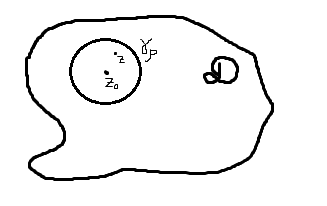
\includegraphics{oblD.png}
\end{wrapfigure}
Пусть $z$ --- произвольная точка круга: $z \in B(z_0; \rho)$. На основании интегральной формулы Коши:

\begin{center}
    $\dfrac{1}{2\pi i}\int\limits_{\gamma_{\rho}}\dfrac{f(\xi)}{\xi - z_0}d\xi = f(z)$
\end{center}

Разложим фукнцию $\dfrac{1}{\xi - z}$ в степенной ряд по степеням $z - z_0$:

\begin{center}
    $\dfrac{1}{\xi - z}$ = $\dfrac{1}{(\xi - z_0) - (z - z_0)} = \dfrac{1}{\xi - z_0}\cdot\dfrac{1}{1 - \dfrac{z - z_0}{\xi - z_0}} = \sum\limits_{n=0}^{\infty}\dfrac{(z - z_0)^n}{(\xi - z_0)^{n + 1}}$
\end{center}

Если $\xi \in \gamma_{\rho}$, то $|\xi - z_0| = \rho$; $|\dfrac{z - z_0}{\xi - z_0}| = \dfrac{|z - z_0|}{\rho} < 1$ и, значит, полученный ряд сходится равномерно на окружности $\gamma_{\rho}$ как ряд от $\xi$.

Ряд $\dfrac{f(\xi)}{\xi - z} = \sum\limits_{n=0}^{\infty}\dfrac{f(\xi)}{(\xi - z_0)^{n+1}}\cdot(z - z_0)^n (*)$ сходится на $\gamma_{\rho}$ равномерно по $\xi$ в силу признака Вейерштрасса ($f$ непрерывна $\Rightarrow |f| \leq M$).

Тогда $|\dfrac{f(\xi)}{(\xi - z_0)^{n+1}}\cdot(z - z_0)^{n}| \leq \dfrac{M}{\rho}\cdot|\dfrac{z - z_0}{\rho}|^n = \dfrac{M}{\rho}\cdot q^n$ - мажоранта. Поэтому этот ряд можно почленно проинтегрировать на $\gamma_{\rho}$.
\par\bigskip
Проинтегрируем (*):

\begin{center}
    $\int\limits_{\gamma_{\rho}}\dfrac{f(\xi)}{\xi - z}d\xi = \sum\limits_{n=0}^{\infty}\int\limits_{\gamma_{\rho}}\dfrac{f(\xi)}{(\xi - z_0)^{n+1}}d\xi\cdot(z - z_0)^n$
\end{center}

Учитывая итегральгую формулу Коши, получим:

\begin{center}
    $f(z) = \sum\limits_{n=0}^{\infty} c_n(z - z_0)^n (2)$, где $c_n ::= \dfrac{1}{2\pi i}\int\limits_{\gamma_{\rho}}\dfrac{f(\xi)}{(\xi - z_0)^{n+1}}d\xi (3)$
\end{center}

Ряд (2) сходится в круге $B(z_0; \rho)$, а это и означает, что $f(\xi)$ регулярна в точке $z_0$. В силу проивола в выборе $z_0$ следует регулярность $f$ в $D$. \quad $\blacksquare$
\par\bigskip
\textbf{Замечание 1.} \quad Понятия дифференцируемости и регулярности функции в области $D$ равносильны, поэтому на регулярные функции автоматически переносятся все свойства функций, дифференцируемых в области, например: линейная комбинация регулярных функций в области есть функция регулярная в той же области, композиция регулярных функций есть функция регулярная и т.д.
\par\bigskip
\textbf{Замечание 2.} \quad Во всех доказательствах и теоремах выше выражение "функция дифференцирума в области $D$" можно теперь заменить на выражение "фукнция регулярна в области $D$". Например, интегральную теорему Коши можно теперь сформулировать следущим образом: \textit{Если функция $f$ регулярна в области $D$ и непрерывна в $\overline{D}$, то $\int\limits_{\partial D}f(z)dz = 0$}.
\par\bigskip
\textbf{Замечание 3.}\quad Следует иметь в виду, что понятие регулярности и дифференцируемости функции в итоге не равносильны. А именно: если функция $f$ регулярна в точке $z_0$, то она дифференцируема в этой точке. Это вытекает из доказательства необходимости в теореме. Обратное же не верно. Функция $f(z) = \overline{z}^2$ дифференцируема в точке 0, но не голоморфна в этой точке. Для того, чтобы функция была голоморфной в точке, нужно чтобы оа была дифференцируема как в самой точке, так и в некоторой окрестности этой точки.
\par\bigskip
\textbf{Замечание 4.} \quad Из доказательства теоремы следует, что ряд (2) заведомо сходится в круге $B(z_0, R)$, где $R$ - расстояние от точки $z_0$ до границы области дифференцируемости функции $f$ (до ближайшей точки недифференцируемости) и не может сходится в большем круге, ибо сумма степенного ряда - функция дифференцируемая в круге сходимости.
\par\bigskip
\textbf{Замечание 5.}\quad Голоморфность функции в бесконечно удалённой точке определяется следующим образом: $f(z)$ называют регулярной в точке $z = \infty$, если функция $g(\xi) = f(\dfrac{1}{\xi})$ голоморфна в точке $\xi = 0$. Отсюда вытекает, что f(z) определённая в некоторой окрестности точки $z = \infty$ будет голоморфной в точке $\z = \infty$ в том и только в том случае, если она представима некоторой окрестности точки $z = \infty$ сходящимся рядом:

\begin{center}
    $f(z) = \sum\limits_{n=0}^{\infty}\dfrac{c_n}{z^b}$
\end{center}


\par\bigskip
\subsection{Интегральное представление для произвольной регулярной функции}

\textbf{Теорема.} \quad
\textit{Если $f$ регулярна в области $D$, то она бесконечное число раз дифференцируема в этой области, причём имеет место формула:}
\begin{center}
    $f^{(n)}(z) = \dfrac{n!}{2\pi i}\int\limits_{\gamma_{\rho}}\dfrac{f(\xi)}{(\xi - z)^{n+1}}d\xi$
\end{center}

$\blacklozenge$ Возьмём $\forall z_0 \in D$. Т.к. $f$ голоморфна в точке $z_0$, то $f(z) = \sum\limits_{n=0}^{\infty}c_n(z - z_0)^n$, где ряд сходится в некотором круге $B(z_0; \rho) \subset D$. Но степенной ряд можно любое число раз дифференцировать в круге сходимости и коэффициенты этого ряда вычисляются по формуле:
\begin{center}
    $c_n = \dfrac{f^{(n)}(z_0)}{n!}$
\end{center}
поскольку степенной ряд является рядом Тейлора своей суммы.
\par\bigskip
С другой стороны, при доказательстве предыдущей теоремы было получено, что:

\begin{center}
    $c_n = \dfrac{1}{2\pi i}\int\limits_{\gamma_{\rho}}\dfrac{f(\xi)}{(\xi - z_0)^{n+1}}d\xi (3)$
\end{center}

В силу единственности разложения функции в степенной ряд получим:

\begin{center}
   $\dfrac{f^{(n)}(z_0)}{n!} = \dfrac{1}{2\pi i}\int\limits_{\gamma_{\rho}}\dfrac{f(\xi)}{(\xi - z_0)^{n+1}}d\xi$
\end{center}

Учитывая произвол в выборе точки $z_0$:

\begin{center}
   $f^{(n)} = \dfrac{n!}{2\pi i}\int\limits_{\gamma_{\rho}}\dfrac{f(\xi)}{(\xi - z)^{n+1}}d\xi$ \quad$\blacksquare$
\end{center}
\par\bigskip
\textbf{Замечание 1.} \quad Если $f$ дифференцируема один раз в некоторой окрестности точки $z_0$, то она дифференцируема сколько угодно раз в этой окрестности.
\par\bigskip
\textbf{Замечание 2.}\quad Формула для вычисления n-й производной функции $f$ может быть получена формальным дифференцированием интегральной формулы Коши, причём дифференцирование производится под знаком интеграла.
\par\bigskip
\textbf{Замечание 3.}\quad Если функция $f$ дифференцируема в окрестности точки $z_0$, то она регулярная в точке $z_0$ и представима степенным рядом, который является рядом Тейлора для $f$. Таким образом, формальный ряд тейлора $\sum\limits_{n=0}^{\infty}\dfrac{f^{(n)}(z_0)}{n!}(z - z_0)^n$ для функции $f$, дифференцируемой в окрестности точки $z_0$ сходится к $f$ в некоторой окрестности точки $z_0$.

\par\bigskip
Аналогичное утверждение для функции действительного переменного не имело место. \par\bigskip Например:
\begin{center}
    $f(x) = $
    \begin{cases}
        $e^{-\frac{1}{x^2}}, x \ne 0$\\
        0, $x = 0$
    \end{cases}
\end{center}
всюду дифференцируема и имеет, в частности, все производные в точке $x = 0$ равные 0 и, значит, все коэффициенты Тейлора в точке $x = 0$ тоже равны 0, однако $f(x)$ тождественно не равна $0$.
\par\bigskip
\textbf{Замечание 4.}\quad Теореме можно придать следующую формулировку:

\textit{Если $f$ регулярна в $D$ и непрерывна в $\overline{D}$, то \exists f^{(n)}(z), \forall z \in $D$ и при этом
\begin{center}
$f^{(n)}(z) = \dfrac{n!}{2\pi i}\int\limits_{\gamma_{\rho}}\dfrac{f(\xi)}{(\xi - z)^{n+1}}d\xi$ 
\end{center}}
\par Доказательство вытекает из доказанной теоремы и следствия 2 к теореме Коши.





\subsection{Теорема Лиувилля}
\textbf{Теорема.} \quad
\textit{Если $f$ ограничена по модулю и регулярна во всей плоскости комплексного переменного, то f(z) = const, $\forall z$}\\
$\blacklozenge$ \hspace{1 mm} Поскольку $f$ регулярна во всей плоскости комплексного переменного, то она дифференцируема при $\forall z$ и производную можно вычистить по формуле:

\begin{center}
    $f'(z) = \dfrac{1}{2\pi i}\int\limits_{\gamma_{\rho}}\dfrac{f(\xi)}{(\xi - z)^2}d\xi$; $\gamma_{\rho} = S(z_0; \rho), \rho > 0$
\end{center}

Оценим $f'(z)$ по модулю, учитывая, что $\forall z: |f(z)| \leq M$:

\begin{center}
    $|f'(z)| \leq \dfrac{1}{2\pi}\int\limits_{\gamma_{\rho}}\dfrac{|f(\xi)|}{\rho^2}d\xi \leq \dfrac{M}{2\pi\rho^2}\cdot2\pi\rho = \dfrac{M}{\rho}$
\end{center}

Т.к. интеграл не зависит от $\rho$, то $\rho$ можно выбрать сколь угодно большим $\Rightarrow$ $|f'(z)| = 0$.

В силу произвола в выборе точки $z$ получаем $|f'(z)| = 0, \forall z \Rightarrow f'(z) = 0 \Rightarrow f(z) = const.$ $\blacksquare$
\par\bigskip
\textit{\textbf{Следствие (Основная теорема алгебры):} Пусть $P_n(z) = c_nz^n + c_{n-1}z^{n-1} + ... + c_1z + c_0, n \geq 1, c_k \in C, c_n \ne 0$ --- некоторый многочлен степени n с комплексными коэффициентами. Тогда $P_n(z)$ имеет по крайней мере 1 комплексный корень.}\\
$\blacklozenge$ \hspace{1 mm} Докажем от противного. Пусть $P_n(z) \ne 0, \forall z$.

Функция $f(z) = \dfrac{1}{P_n(z)}$ будет голоморфной во всей комплексной плоскости. $P_n(z) \rightarrow \infty$ при $z \rightarrow \infty \Rightarrow f(z) \rightarrow 0$ при $z \rightarrow \infty \Rightarrow \exists M: |f(z)| \leq M, \forall z$. По теореме Лиувилля $\Rightarrow f(z) = const \Rigtharrow P_n(z) = const$. Это противоречит тому, что $c_n \ne 0$. $\blacksquare$

\par\bigskip
\textbf{Пример. } \quad $sinz, cosz$ в силу теоремы Лиувилля не ограничены в плоскости комплексных чисел. 

\subsection{Теорема Мореры}

\textbf{Теорема. }\quad
\textit{Если $f$ непрерывна в одгосвязной области $D$ и интеграл от $f$ по любому замкнутому контуру, лежащему в $D$, равен 0 ($\int\limits_{l}f(z)dz = 0$), то функция $f$ регулярна в области $D$}.\\
$\blacklozenge$\hspace{2 mm} Как известно, непрерывная в области $D$ функция, интграл от которой по любому замкнутому контуру равен нулю, обладает в этой области первообразной, т.е. $\exists F(z)$ такая, что $F'(z) = f(z)$. По критерию регулярности $F(z)$ - регулярна в $D$ и, следовательно, её производная регулярна в $D$, т.е. $F'(z) = f(z)$ - регулярна в $D$. $\blacksquare$
\par\bigskip
\textbf{Замечание. }\quad Эта теорема в некотором смысле является обратной к интегральной теореме Коши. Она даёт достаточные условия регулярности функции.

\par\bigskip
\textbf{Пример. } \quad
\begin{wrapfigure}[4]{r}{0.2\linewidth} 
    \vspace{-5ex}
    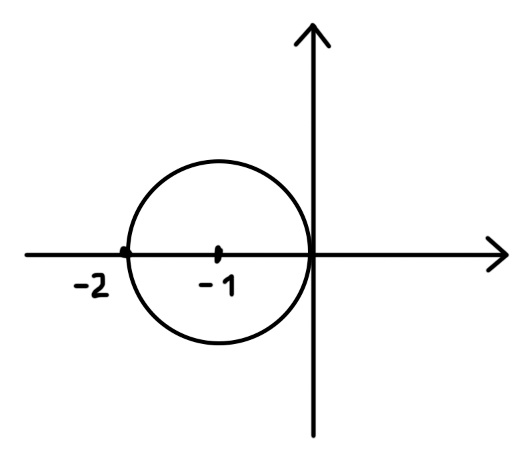
\includegraphics[width=0.2\textwidth]{luivill.png}
\end{wrapfigure}
\textit{1) Вычислить $J = \int\limits_{|z+1|=1}\dfrac{z^2}{z^2 + 4z + 3}dz$}
\\
$J = \int\limits_{|z+1|=1}\dfrac{z^2}{(z + 1)(z + 3)}dz = \int\limits_{|z+1|=1}\dfrac{\dfrac{z^2}{z + 3}}{(z + 1)}dz = 2\pi i \dfrac{z^2}{z + 3}\bigg|_{z = -1} = 2\pi i \dfrac{1}{2} = \pi i$




\subsection{Первая теорема Вейерштрасса}

\textit{Как мы уже имели возможность убедиться, регулярные функции обладают свойствами, которым нет аналога у действительных функций. В частности, может быть значительно усилена и теорема о дифференцировании рядов функций по сравнению с соответствующей теоремой для действительных рядов. Напомним, что мы уже отмечали, что теорема о непрерывности суммы ряда функций и теоремы об интегрировании звучали так же.}
\par\bigskip
 \textbf{Теорема (первая теорема Вейерштрасса).}\quad
\textit{Если $f_n$ регулярны в области $D$, а ряд $\sum\limits_{n=1}^{\infty} f_n(z) = f(z)$ сходится равномерно в любой замкнутой области $\overline{G}$, где $G \subset D$, то:}
\begin{enumerate}
    \item \textit{$f = \sum f_n$ - есть функция регулярная в $D$}
    \item \textit{Ряд можно дифференцировать почленно в $D$ любое число раз,} \par \textit{т.е. $f^{(k)}(z) = \sum\limits_{n=1}^{\infty}f_n^{(k)}(z), k \in N$;}
    \item \textit{Ряд из производных $\sum f_n^{(k)}(z)$ сходится равномерно в любой замкнутой области $\overline{G} \subset D$ (сходится локально-равномерно в $D$).}
\end{enumerate} \\
$\blacklozenge$ 1) По теореме, являющейся аналогом теоремы Стокса-Зейделя, $f$ является функцией непрерывной в любой замкнутой области $\overline{G} \subset D$, откуда следует, что она непрерывна в $D$, поскольку любая точка $z \in D$ является внутренней и поэтому может быть заключена в некоторую $\overline{G} \in D$. На основании теоремы о почленном интегрировании ряд можно интегрировать почленно по любой спрямляемой прикой из $C$. В частности:

\begin{center}
    $\int\limits_l f(z)dz = \sum\limits_{n=1}^{\infty}\int\limits_l f_n(z)dz$,
\end{center}

где $l$ - замкнутый спрямляемый контур из $D$. Т.к. функции $f_n(z)$ регулярны в $D$, то $\int\limits_l f_n(z)dz = 0$ для $\forall n \in N$ и поэтому и $\int\limits_l f(z)dz = 0$. По теореме Мореры, $f(z)$ регулярна в $D$.
\par\bigskip
2) Зафиксируем любую точку $z \in D$ и построим круг $B(z; \rho)$ так, чтобы $\overline{B}(z; \rho) \subset D; \gamma_{\rho} ::= S(z; \rho)$, тогда на основании интегральной формулы Коши для производной поскольку все $f_n(z)$ и $f(z)$ регулярны в $\overline{B}(z; \rho)$, то:

\begin{center}
    $f^{(k)}(z) = \dfrac{k!}{2\pi i} \int\limits_{\gamma_{\rho}}\dfrac{f(\xi)}{(\xi - z)^{k+1}}d\xi$ (1)
    \par\bigskip
    $f_n^{(k)}(z) = \dfrac{k!}{2\pi i} \int\limits_{\gamma_{\rho}}\dfrac{f_n(\xi)}{(\xi - z)^{k+1}}d\xi$ (2)
    \par\bigskip
    $k \in N, k - fix$
\end{center}
\par\bigskip
Поскольку ряд $\sum\limits_{n=1}^{\infty}f_n(\xi)$ сходится равномерно на $\gamma_{\rho}$, то на $\gamma_{\rho}$ сходится равномерно и ряд $\sum\limits_{n=1}^{\infty}\dfrac{f_n(\xi)}{(\xi - z)^{k+1}}$. Действительно, для остатка этого ряда, учитывая, что $|\xi - z| = \rho$ будем иметь следующую оценку ($r_n(\xi)$ - остаток первого ряда, $R_n(\xi)$ - остаток исследуемого ряда):

\begin{center}
    $|R_n(\xi)| = \dfrac{1}{|\xi - z|^{k+1}}|r_n(\xi)| = \dfrac{1}{\rho^{k+1}}|r_n(\xi)| \leq \dfrac{\epsilon}{\rho^{k+1}}$,
\end{center}

где $\rho, k$ - постоянные, $\forall \xi \in \gamma_{\rho}$.

Следовательно, указанный ряд можно интегрировать почленно на $\gamma_{\rho}$. Проинтегрируем тождество

\begin{center}
    $\dfrac{f(\xi)}{(\xi - z)^{k+1}} = \sum\limits_{n=1}^{\infty}\dfrac{f_n(\xi)}{(\xi - z)^{k+1}}$
\end{center}

вдоль $\gamma_{\rho}$. Получим:

\begin{center}
    $\int\limits_{\gamma_{\rho}}\dfrac{f(\xi)}{(\xi - z)^{k+1}} = \sum\limits_{n=1}^{\infty}\int\limits_{\gamma_{\rho}}\dfrac{f_n(\xi)}{(\xi - z)^{k+1}}$
\end{center}

Учитывая (1) и (2) в итоге получаем:

\begin{center}
    $f^{(k)}(z) = \sum\limits_{n=1}^{\infty}f_n^{(k)}(z)$
\end{center}

3) Покажем, что $\sum\limits_{n=1}^{\infty}f_n^{(k)}(z)$ сходится равномерно $\forall \overline{G} \in D$. Действительно, поместим $\overline{G}$ в контур $l$ так, чтобы $l \in D$. 
\par\bigskip\par\bigskip
\begin{wrapfigure}[4]{l}{0.5\linewidth} 
    \vspace{-5ex}
    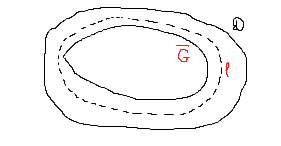
\includegraphics{GinDVeyerhtrass.png}
\end{wrapfigure}

Обозначим за $P$ область, ограниченную контуром $l$. Обозначим $d ::= \rho(\overline{G}, l) > 0$. Тогда $\forall \xi \in l, \forall z \in \overline{G}: |\xi - z| \geq d$. Т.к. $r_n(z)$ --- остаток ряда $\sum\limits_{n=1}^{\infty}f_n(z)$ есть функция регулярная (т.к. $r_n(z) = f(z) - \sum\limits_{p=1}^n f_p(z), f(z) регулярна по пункту 1 теоремы, а \sum\limits_{p=1}^n f_p(z) регулярна как сумма конечного числа регулярных функций$), то $\forall z \in \overline{G}$ имеет место равенство:

\begin{center}
    $r_n^{(k)}(z) = \dfrac{k!}{2\pi i}\int\limits_{l}\dfrac{r_n(\xi)}{(\xi - z)^{k+1}}d\xi$
\end{center}

По условию, ряд $\sum f_n(z)$ сходится равномерно в замкнутой области $\overline{D}$, ограниченной контуром $l$, поэтому $\forall \varepsilon > 0, \exists \nu(\varepsilon) > 0, \forall n \geq \nu(\varepsilon), \forall z \in \overline{D} \Rightarrow |r_n(z)| \leq \varepsilon$.

Пусть теперь $n \geq \nu(\varepsilon)$. Тогда $|r_n^{(k)}| = \dfrac{k!}{2\pi}|\int\limits_l \dfrac{r_n(\xi)}{(\xi - z)^{k+1}}\,d\xi| \leq \dfrac{k!}{2\pi}\int\limits_l\dfrac{|r_n(\xi)|}{|\xi - z|^{k+1}}d\xi \leq \dfrac{k! \cdot \varepsilon}{2\pi \cdot d^{k+1}} \cdot$дл$l = k\cdot \varepsilon$, что и доказывает равномерную сходимость ряда $\sum f_n^{(k)}(z)$ в области $\overline{G}$. $\blacksquare$
\par\bigskip
\textbf{Замечание 1.}\quad Теорема, очевидно, имеет место, если потребовать равномерную сходимость ряда $\sum f_n(z)$ в $\overline{D}$.
\par\bigskip
\textbf{Замечание 2.} \quad Как показывает простой пример, из равномерной сходимости ряда $\sum f_n(z)$ в $\overline{D}$ не следует равномерная сходимость в $\overline{D}$ ряда из производных:

$\sum\dfrac{z^n}{n^2}$ сходится равномерно в $\overline{B}(0; 1)$, а ряд $\sum\dfrac{z^{n-1}}{n}$ уже не будет равномерно сходящимся в круге $\overline{B}(0; 1)$, т.к. он и вовсе расходится при $z = 1$. Другими словами, заключение 3) теоремы не может быть, вообще говоря, расширено.  



\par\bigskip
\subsection{Вторая теорема Вейерштрасса}

\textbf{Теорема (вторая теорема Вейерштрасса)} \quad
\textit{Если $f_n(z)$ регулярны в $D$, непрерывны в $\overline{D}$ и $\sum\limits_{n=1}^{\infty}f_n(z)$ сходится равномерно на $\partial D$, то он сходится равномерно и в $\overline{D}$}. \bigskip \\
$\blacklozenge$ \hspace{1 mm} Воспользуемся критерием Коши равномерной сходимости. \par Т.к. $\sum f_n(z)$ сходится равномерно на $\partial D$, то $$\forall \varepsilon > 0, \exists \nu(\varepsilon) > 0, \forall n \geq \nu(\varepsilon), \forall p \geq 0, \forall \xi \in \delta D \quad \Rightarrow \quad |\sum\limits_{k=n+\xi}^{n+p}| \leq \varepsilon$$.

Рассмотрим функцию $g(z) = \sum\limits_{k=n}^{n+p}f_k(z)$. Эта функция регулярна в $D$ и непрерывна в $\overline{D}$ как сумма конечного числа функций, обладающих этими же свойствами. По теореме о максимуме модуля регулярной функции:

\begin{center}
    $|g(z)| = |\sum\limits_{k=n}^{n+p}f_k(z)| \leq \max\limits_{s \in \partial D}|\sum\limits_{k=n}^{n+p}f_k(z)| \leq \varepsilon$
\end{center}

Т.е. для $\sum f_n(z)$ в $\overline{D}$ выполняется критерий Коши равномерной сходимости.  $\blacksquare$ 

\par\bigskip
\subsection{Разложение регулярных функций в ряды Тейлора}
\par\bigskip
Как уже отмечалось, дифференцируемая в некоторой окрестности точки $z_0$ (включая саму $z_0$) функция $f$ может быть представлена рядом Тейлора:

\begin{center}
    $f(z) = \sum_{n=0}^{\infty}c_n(z - z_0)^n$,
\end{center}

где коэффициенты $c_n$ могут быть вычислены по формулам:

\begin{center}
    $c_n = \dfrac{f^{(n)}(z_0)}{n!}$,
\end{center}

либо

\begin{center}
    $c_n = \dfrac{1}{2\pi i}\int\limits_{\gamma_{\rho}}\dfrac{f(\xi)}{(\xi - z_0)^{n+1}}d\xi$,
\end{center}

$\gamma_{\rho} = S(z_0; \rho)$ лежит в области регулярности $f$. Радиус сходимости ряда может быть вычислен \textbf{по формулам Коши-Адамара}:

\begin{center}
    $R = \dfrac{1}{\overline{\lim}\sqrt[n]{|c_n|}}$, либо $R = \lim|\dfrac{c_n}{c_{n+1}}|$
\end{center}

Отметим, что на границе круга сходимости функция не может быть регулярной во всех точках, ибо допуская противное, окажется, что каждая точка окружности обдалает окрестностью, в которой функция регулярна, а тогда можно доказать, что $\exists r$, что $f$ будет регулярна в круге радиуса $R + r$ с центром в точке $z_0$, что противоречит тому, что $R$ - радиус сходимости. Кстати, это согласуется и с замечанием к теореме о связи регулярных и дифференцируемых функций, где утверждалось, что радиус сходимости равен расстоянию от точки $z_0$ до границы области дифференцируемости (до ближайшей точки недиффиренцируемости).
\par\bigskip
Точку, в которой $f$ регулярна, называют \textbf{регулярной (обыкновенной, правильной)} точкой функции $f$. Все остальные точки будем называть \textbf{особыми}. Например, $w = \ln(z), z = 0$ --- особая, все остальные --- регулярные.
\par\bigskip
Итак:\; \textit{Если $z_0$ --- правильная точка для $f$, то $f$ может быть представлена степенным рядом с центром в этой точке: $f(z) = \sum\limits_{n=0}^{\infty}c_n(z - z_0)^{n},$ причём радиус сходимости этого ряда равен расстоянию от точки $z_0$ до ближайшей особой точки функции $f$}.
\par\bigskip
\textbf{Примеры: }
\begin{enumerate}
    \item  В области действительных чисел не совсем ясно было, почему ряд $\dfrac{1}{1 + x^2} = \sum\limits_{n=0}^{\infty}(-1)^n x^{2n}$ расходится вне интервала $]-1; 1[$, в то время как $\dfrac{1}{1 + x^2}$ определена, непрерывна и дифференцируема сколько угодно раз на всей действительной оси, причём точки $x = \pm 1$ для неё не являются особыми. \par Теперь картина ясна: у функции $\dfrac{1}{1 + x^2}$ точки $z = \pm i$ являются особыми, а поэтому радиус сходимости $R = 1$.
    
    \item $\sum\dfrac{z^n}{n^2}, R = 1$ и хотя в $\overline{B}(0; 1)$ ряд сходится равномерно, на $S(0; 1)$ лежит по крайней мере одна особая точка функции, являющейся суммой этого ряда.
    \par

    Отметим в заключение, что для элементарных функций $\sin(z), \cos(z), \ln(1 + z), \sh(z), \ch(z),$
    $ e^z, \dfrac{1}{1 + z}$ имеют место основные разложения в ряды Тейлора, знакомые нам с действительного анализа.
\end{enumerate}





\subsection{Нули регулярной функции}
Точка $z = z_0$ называется \textbf{нулём} функции $f(z)$, регулярной в этой точке, если $f(z) = 0$.
\par\bigskip
Пусть $z_0$ --- нуль функции $f(z)$ и $z_0 \ne \infty$. Представим $f$ степенным рядом в окрестности точки $z = z_0$, что возможно, поскольку $f$ голоморфна в этой точке:

\begin{center}
    $f(z) = \sum\limits_{n=0}^{\infty}c_n(z - z_0)^n$
\end{center}

Поскольку $z_0$ --- нуль функции $f$, то $f(z_0) = c_0 = 0$. Пусть $c_m$ --- первый отличный от нуля коэффициент в написанном разложении, т.е.:

\begin{center}
    $f(z) = \sum\limits_{n=m}^{\infty}c_n(z - z_0)^n = c_m(z - z_0)^m + c_{m+1}(z - z_0)^{m+1} + ..., c_m \ne 0$
\end{center}

Тогда число $m$ называют \textbf{порядком} или \textbf{кратностью} нуля $z = z_0$ функции $f$.
\par\bigskip
Т.к. $c_n = \dfrac{f^{(n)}(z_0)}{n!}$, то порядок нуля равен наименьшему порядку производной функции $f$ в этой точке, отличной от нуля.
\par\bigskip
Функцию $f$ можно переписать иначе:

\begin{center}
    $f(z) = (z - z_0)^m (c_m + c_{m+1}(z - z_0) + ...)$
\end{center}

где ряд $c_m + c_{m+1}(z - z_0) + ... =:: g(z)$ сходится в том же круге, что и ряд для $f$. Поэтому его сумма, т.е. функция $g(z)$ регулярна в точке $z_0$ и $g(z_0) = c_m \ne 0$.
\par\bigskip
Таким образом, если $z = z_0$ --- нуль регулярной функции $f(z)$ порядка $m$, то справедливо представление:

\begin{center}
    $f(z) = (z - z_0)^m g(z), g(z_0) \ne 0, g$ --- регулярна в точке $z = z_0$.
\end{center}

Нетрудно видеть, что справедливо и обратное утверждение. Отсюда получаем четыре маленьких следствия:
\par\bigskip
\textbf{Следствие 1.}\quad Нули регулярной функции всегда имеют целый порядок.
\par\bigskip
\textbf{Следствие 2.} \quad Для того, чтобы $z_0$ была нулём функции $f(z)$ необходимо и достаточно, чтобы при $z \rightarrow z_0: f(z) \sim A \cdot (z - z_0)^m$
\par\bigskip
\textbf{Следствие 3.} Если $z = z_0$ --- нуль порядка $m$ функции $f$, то для $(f(z))^k, k \in N, z_0$ является нулём порядка $m \cdot k$.
\par\bigskip
\textbf{Следствие 4.}\quad Если $z_0$ --- нуль порядка $m$ функции $f$, то для $f' z_0$ будет нулём порядка $m - 1$.
\par\bigskip

Рассмотрим теперь случай, когда $z = \infty$ --- нуль функции $f(z)$, т.е. $f(\infty) = 0$ и функция $f$ регулярна в точке $z = \infty$. Тогда, как мы знаем, в окрестности $z = \infty$ функция $f$ может быть представлена рядом:

\begin{center}
    $f(z) = \sum\limits_{n=1}^{\infty}\dfrac{c_n}{z^n}$
\end{center}

Если $c_m$ --- первый отличный от нуля коэффициент в этом разложении, то $m$ называют порядком или кратностью нуля $z = \infty$ функции $f$.

Тогда $f(z) = \dfrac{1}{z^m}(c_m + \dfrac{c_{m+1}}{z} + ...) = \dfrac{1}{z^m}\phi(z)$, где $\phi(z)$ --- функция, регулярная в бесконечно удалённой точке и $\phi(\infty) = c_m \ne 0$.

Верно и обратное: если $f$ представима в виде $f(z) = \dfrac{\phi(z)}{z^m}$, где $\phi(z)$ - регулярная и $\phi(\infty) \ne 0$, то $z = \infty$ является нулём кратности $m$ функции $f$.

Отметим, что и в этом случае нули имеют целый порядок, а так же, при $z \rightarrow \infty f(z) \sim \dfrac{B}{z^m}$.
\par\bigskip
\textbf{Примеры.} \quad Найти нули и определить их порядок:
\begin{enumerate}
    \item $f(z) = \sin(z)$. $z = 0$ - нуль первого порядка, т.к. $\sin(z) \sim z$ при $z \rightarrow0$. Также $z = k\pi, k \in Z$ --- нули первого порядка, т.к. $f'(k\pi) = cos(k\pi) \ne 0, \forall k \in Z$
    \item $\dfrac{(z^3 + 1)^4}{(z^2 + 7)^11}e^{\dfrac{1}{z}} \sim_{z \rightarrow \infty} \dfrac{z^{12}}{z^{22}} = \dfrac{1}{z^{10}} \quad \Rightarrow \quad z = \infty$ --- нуль 10-го порядка.
    \item $(e^z - 1)^3 \sim z^3 \quad \Rightarrow \quad z = 0$ --- нуль третьего порядка.
\end{enumerate}
\par\bigskip


Для нулей регулярных фукнций имеет место одна очень интересная теорема: 
\par\bigskip
\textbf{Теорема.} \quad
\textit{Пусть $f$ регулярна в точке $z_0$ и $f(z_0) = 0$. Тогда, либо $f(z) \equiv 0$ в некоторой окрестности точки $z_0$, либо $\exists$ такая окрестсность точки $z_0$, в которой нет нулей функции $f(z)$, отличных от $z_0$ (т.е. обязательно будет существовать такая окрестность точки $z_0$, в которой не будет таких точек $z$ (кроме неё самой), в которых функция $f$ обащается в нуль).}\\
$\blacklozenge$ \hspace{1 mm} $f(z) = \sum\limits_{n=1}^{\infty}c_n(z - z_0)^n, z \in B(z_0; \rho), \rho > 0$.
\par\bigskip
Возможны два случая:
\par\bigskip
1) Все $c_k = 0, k \in N \Rightarrow f(z) = 0, \forall z \in B(z_0; \rho)$
\par\bigskip
2) $\exists m \geq 1$ такое, что $c_0 = c_1 = ... = c_{m-1} = 0, c_m \ne 0$. Тогда $z_0$ --- нуль кратности $m$ функции $f$ и $f(z) = (z - z_0)^m g(z), g(z_0) \ne 0, g$ --- регулярна в точке $z_0$. В силу непрерывности функции в некоторой окрестности $z_0$ из условия $g(z_0) \ne 0 \Rightarrow g(z) \ne 0$ в некоторой окрестности точки $z_0$. Итак, $\exists$ окрестность точки $z_0$, в которой нет других нулей функции $f$, кроме самой $z_0$. \quad $\blacksquare$ 
\par\bigskip
Короче теорему можно сформулировать так: \textit{нули регулярной функции изолированы}.




\section{Множество сходимости ряда Лорана}
\textbf{Рядом Лорана} называют ряд вида:
\par\bigskip
\begin{center}
  $$  \sum_{n = -\infty}^{+\infty} c_n (z - z_0)^n  \eqno(1) $$
\end{center}
\par\bigskip
Где $z_0$ - фиксированная точка комплексной плоскости, $c_n$ - комплексные числа, зависящие от n и не зависящие от $z$. Суммирование ведётся как по положительным так и по отрицательным значениям индекса $n$.
\par\bigskip
В развёрнутой форме ряд Лорана можно исследовать как сумму двух рядов:
\begin{center}
  $$  \sum_{n = 0}^{+\infty} c_n (z - z_0)^n = f_1(z)  \eqno(2) $$
  \par
  $$  \sum_{n = -\infty}^{-1} c_n (z - z_0)^n = \sum_{n = 1}^{+\infty} c_{-n} \frac{1}{(z - z_0)^n} = f_2(z)  \eqno(3) $$
\end{center}
\par\bigskip
и тогда:
\par\bigskip
\begin{center}
  $$\sum_{n = -\infty}^{+\infty} c_n (z - z_0)^n = \sum_{n = 1}^{+\infty} c_{-n} \frac{1}{(z - z_0)^n} + \sum_{n = 0}^{+\infty} c_n (z - z_0)^n$$
\end{center}
\par\bigskip
Ряд (1) называется сходящимся в точке $z$, если в этой точке одновременно сходятся ряды (2) и (3) и в случае сходимости под суммой ряда понимают:
\begin{center}
  $f(z) = f_1(z) + f_2(z)$
\end{center}

Исследование сходимости ряда Лорана сводится к исследованию сходимости двух степенных рядов.
\par
Ряд (2), как известно, сходится в круге $B(z_0, R) = \{z $ $|$ $ |z - z_0| < R\}$ где $R$ - радиус сходимости $R = \frac{1}{lim_{n \to \infty} \sqrt{|c_n|}}$
\par\bigskip
Рассмотрим ряд (3). Сделав замену $\frac{1}{z - z_0} = \xi$ приходим к степенному ряду по степеням $\xi$: 
$$\sum_{n = 1}^{+\infty} c_{-n} \xi^n$$
\par\bigskip
Он сходится в круге $B(0, \frac{1}{r})$, где через $\frac{1}{r}$ обозначен радиус сходимости:
\par\bigskip
$$\frac{1}{r} = \frac{1}{lim_{n \to \infty} \sqrt{|c_{-n}|}}$$
\par\bigskip
Т.е. ряд сходится для таких $\xi$, что $|\xi| < \frac{1}{r}$ и, следовательно, для ряда (3) получаем:
$|\xi| = \frac{1}{|z - z_0|} < \frac{1}{r} \Rightarrow |z - z_0| < r$. Ряд сходится вне круга $B(z_0, r)$.
\par\bigskip
Т.к. ряд Лорана сходится, когда одновременно сходятся ряды (2) и (3), то возможны три случая:
\par\bigskip
\begin{figure}[bh]
\begin{minipage}[t]{0.32\linewidth}
\center{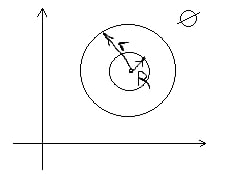
\includegraphics[width=0.8\linewidth]{loran/1.jpg}}
\end{minipage}
\hfill
\begin{minipage}[t]{0.32\linewidth}
\center{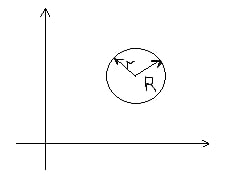
\includegraphics[width=0.8\linewidth]{loran/2.jpg}}
\end{minipage}
\hfill
\begin{minipage}[t]{0.32\linewidth}
\center{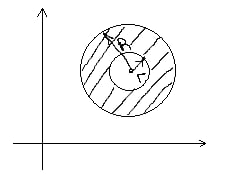
\includegraphics[width=0.8\linewidth]{loran/3.jpg}}
\end{minipage}
\begin{minipage}[t]{1\linewidth}
\begin{tabular}{p{0.32\linewidth}p{0.32\linewidth}p{0.32\linewidth}}
\centering 1) $r < R$  & \centering 2) $r = R$ & \centering 4) $r > R$ 
\end{tabular}
\end{minipage}
\end{figure}
\par\bigskip
Т.е. область сходимости ряда лорана - кольцо:
\par\bigskip
\begin{center}
$B(z_0; r; R) = \{z \, | \,  r < |z - z_0| < R\}$
\end{center}
\par\bigskip
В каждой точке $\mathbb{C} \setminus B(z_0; r, R)$ ряд Лорана расходится, поскольку расходится один из его рядов (2) ил (3)
\par
Если $r = 0$ то $B(z_0; 0, R) = B(z_0, R) \setminus \{z_0\}$
\par
В граничных точках кольца ряд Лорана может как сходиться так и расходиться. Ряд Лорана сходится абсолютно и локально равномерно в кольце $\Rightarrow$ его сумма в кольце сходимости - голоморфная функция.


\section{Представление функций рядом Лорана}
\textbf{Теорема.} \quad
\textsl{Функция $f$ голоморфная в кольце $B(z_0; r, R)$ представима в этом кольце сходимости рядом Лорана: }
\begin{center}
$$ f(z) = \sum_{n = -\infty}^{+\infty} c_n (z - z_0)^n  \eqno(4) $$ 
\end{center}
\par\bigskip
\textsl{где коэффиценты $c_n$ определяются по формуле: }
\begin{center}
\textsl{$$ c_n = \frac{1}{2\pi i} \int_{\varrho_\rho} \frac{f(\xi)}{(\xi - z_0)^{n + 1}}\,d\xi \eqno(5) $$ } 
\end{center}
\par\bigskip
$\varrho_\rho = S(z_0, \rho) \subset B(z_0; r, R)$ $ n \in \mathbb{Z}$
\textsl{, обход в положительном напрвлении.}
\par\bigskip
$\blacklozenge$ Возьмём $\forall z \in B(z_0; r, R)$ и построим кольцо $B(z_0; r_1, R_1)$ так, чтобы $z \in B(z_0; r_1, R_1)$. В силу интегральной теоремы Коши для неодносвязной области получим:
\begin{center}
$$ f(z) = \frac{1}{2\pi i} \int_{\varrho_{R_1}} \frac{f(\xi)}{\xi - z}\,d\xi - \frac{1}{2\pi i} \int_{\varrho_{r_1}} \frac{f(\xi)}{\xi - z}\,d\xi\eqno(6) $$ 
\end{center}
\par
где 
\begin{center}
$\varrho_{R_1} = S(z_0, R_1), $ $\varrho_{r_1} = S(z_0, r_1) $ 
\end{center}
\par\bigskip
и обе окружности обходятся против часовой стрелки.
\par
Рассмотрим каждый из интегралов в отдельности:
\begin{center}
$\frac{1}{2\pi i} \int_{\varrho_{R_1}} \frac{f(\xi)}{\xi - z}\,d\xi = \frac{1}{2\pi i} \int_{\varrho_{R_1}} \frac{f(\xi)}{\xi - z_0} \cdot \frac{1}{1 - \frac{z - z_0}{\xi - z_0}}\,d\xi = $ 
\par\bigskip
$ = \frac{1}{2\pi i} \int_{\varrho_{R_1}} \frac{f(\xi)}{\xi - z_0} \cdot \sum_{n = 0}^{+\infty} \frac{(z - z_0)^n}{(\xi - z_0)^n}$ = [можно проинтегрировать ряд почленно в силу равномерной сходимости] = $$\sum_{n = 0}^{+\infty} c_n(z - z_0)^n \eqno(7)$$
\end{center} \par
где 
\begin{center}
$$c_n = \frac{1}{2\pi i} \int_{\varrho_{R_1}} \frac{f(\xi)}{(\xi - z_0)^{n + 1}}\,d\xi \eqno(8)$$
\end{center}
\par\bigskip
Отметим, что, вообще говоря, мы не можем написать $c_n = \frac{f^{(n)}(z_0)}{n!}$, т.к. $f(z)$ не регулярна в круге $B(z_0, z)$.
\par
В силу теоремы коши для неодносвязной области:
\begin{center}
$$c_n = \frac{1}{2\pi i} \int_{\varrho_\rho} \frac{f(\xi)}{(\xi - z_0)^{n + 1}}\,d\xi \eqno(9)$$
\end{center}
\par
где $\varrho_\rho = S(z_0, \rho) \subset B(z_0; r, R)$.
\par
Рассмотрим второй интеграл из (6):
$$-\frac{1}{2\pi i} \int_{\varrho_{r_1}} \frac{f(\xi)}{\xi - z}\,d\xi = \frac{1}{2\pi i} \int_{\varrho_{r_1}} \frac{f(\xi)}{z - z_0} \cdot \frac{1}{1 - \frac{\xi - z_0}{z - z_0}}\,d\xi = $$
$$ \frac{1}{2\pi i} \int_{\varrho_{r_1}} \sum_{n = 1}^{+\infty} \frac{f(\xi)}{(z - z_0)^n} \cdot (z - z_0)^{n-1}\, d\xi = \sum_{n = -1}^{-\infty} c_n(z - z_0)^n \eqno(10)$$

\par\bigskip
где 
$$c_{-n} = \frac{1}{2\pi i} \int_{\varrho_{r_1}} f(\xi)(\xi - z_0)^{n - 1}\,d\xi$$
\par\bigskip
или

$$c_n = \frac{1}{2\pi i} \int_{\varrho_{r_1}} \frac{f(\xi)}{(\xi - z_0)^{n + 1}}\,d\xi$$
\par\bigskip
В силу теоремы Коши для многосвязных областей:
\begin{center}
$$c_n = \frac{1}{2\pi i} \int_{\varrho_\rho} \frac{f(\xi)}{(\xi - z_0)^{n + 1}}\,d\xi \eqno(11)$$
\end{center}
\par\bigskip
Объединяя всё вместе, получаем:
$$ f(z) = \sum_{n = -\infty}^{+\infty} c_n (z - z_0)^n $$
\par\bigskip
где

$$ c_n = \frac{1}{2\pi i} \int_{\varrho_\rho} \frac{f(\xi)}{(\xi - z_0)^{n + 1}}\,d\xi $$

\par\bigskip
В силу произвольного выбора точки $z$ разложение имеет место в кольце $B(z_0; r, R)$.
$\blacksquare$


\section{Свойства ряда Лорана}
\begin{enumerate}
    \item \textsl{Если $f$ голоморфна в круге $B(z_0; R)$, то все $c_{-n} = 0$ в силу т. Коши и ряд Лорана становится рядом Тейлора. Ряд Тейлора - частный случай ряда лорана.}
    \item \textsl{Разложение в ряд Лорана функции $f$ голоморфной в кольце $B(z_0; r, R)$ единственно.}

$\blacklozenge$\hspace{1 mm} Предположим, что на ряду с представлением 
\begin{center}
$$ f(z) = \sum_{n = -\infty}^{+\infty} c_n (z - z_0)^n $$
\end{center}
\par\bigskip
в этом же кольце имеет место представление
\begin{center}
$$ f(z) = \sum_{n = -\infty}^{+\infty} a_n (z - z_0)^n $$
\end{center}
\par тогда
\begin{center}
$$ \sum_{n = -\infty}^{+\infty} c_n (z - z_0)^n = \sum_{n = -\infty}^{+\infty} a_n (z - z_0)^n $$
\end{center}
\par\bigskip
Умножим это равенство на $(z - z_0)^{- m - 1}$ и проинтегрируем по $\varrho_\rho = S(z_0, \rho) \subset B(z_0, r, R)$:
\begin{center}
$$ \sum_{n = -\infty}^{+\infty} c_n (z - z_0)^{n - m - 1} = \sum_{n = -\infty}^{+\infty} a_n (z - z_0)^{n - m - 1} $$
\end{center}
\par\bigskip
Учитывая, что $\int_{\varrho_\rho} \frac{1}{(z-z_0)^k}\, dz = \begin{cases}
    \ 2\pi i, k = 1 \\
    \ 0, k \in \mathbb{Z} \setminus \{1\}
    \end{cases}$
получим $2\pi i c_m = 2\pi i a_m$ $\Rightarrow c_m = a_m$ $\forall m \in \mathbb{Z}$ $\blacksquare$
\par\bigskip
Отсюда следует, что коэффиценты разложения в ряд Лорана не зависят от того, каким способом это разложение получено. На практике стремятся обойтись без вычисления $c_n$ с помощью интегралов. {\tiny{я хачу питсу}}
\par\bigskip

\item \textsl{Кольцо сходимости ряда Лорана для функции $f$, его размеры, зависят от особых точек функции $f$. Поскольку ряд Лорана можно трактовать как сумму двух степенных рядов, то такими же рассуждениями, как и для ряда Тейлора, можно показать, что каждая из окружностей, являющаяся границей кольца максимальной ширины, внутри которого функцию можно разложить в ряд Лорана, содержит хотя бы одну особую точку функции $f$.}

\item \textsl{\textbf{Неравенство коши для коэффицентов ряда Лорана}}
\par
\textsl{Пусть $f$ голоморфна в кольце $B(z_0, r, R)$, тогда коэффиценты $c_n$ ряда Лорана для $f$ в этом кольце удоволетворяют неравенствам:}
\par\bigskip
\begin{center}
$|c_n| \le \frac{M}{\rho^n}$
\end{center}
\par\bigskip
где $$M = \max_{\varrho_\rho} |f(\xi)|, \varrho_\rho = S(z_0, \rho) \subset B(z_0; r, R)$$
\par\bigskip
$\blacklozenge$ $c_n = \frac{1}{2\pi i} \int_{\varrho_\rho} \frac{f(\xi)}{(\xi - z_0)^{n + 1}}\,d\xi \Rightarrow |c_n| \le \frac{1}{2\pi i} \int_{\varrho_\rho} \frac{|f(\xi)|}{|\xi - z_0|^{n + 1}}\,d\xi \le \frac{M}{2\pi \rho^{n + 1}}\cdot$ $ 2\pi \rho = \frac{M}{\rho^n} $ $\blacksquare$

\item \textsl{Разложение одной и той же функции $f$ в ряд Лорана возможно в разных областях и эти разложения различны.}


\par\bigskip
\textbf{Пример}
\par\bigskip
$f(z) = \frac{1}{(z+1)(z+2)}$ -- разложить в ряд Лорана в окрестности точки $z_0 = 0$. $f$ голоморфна в областях 1) $B(0, 1)$, 2) $B(0, 1, 2)$, 3) $B(0, 2, +\infty).$
\par\bigskip
1) т.к. $f$ регулярна в круге $B(0, 1)$, то ряд Лорана - это ряд Тейлора:
$$\frac{1}{(z+1)(z+2)} = \frac{1}{(z+1)} - \frac{1}{(z+2)} = \sum_{n = 0}^{+\infty} (-1)^n z^n - \sum_{n = 0}^{+\infty} \frac{(-1)^n z^n}{2^{n + 1}} = \sum_{n = 0}^{+\infty} (-1)^n (1 - \frac{1}{2^{n + 1}}) z^n$$
\par\bigskip
2) $B(0, 1, 2)$ 
$$\frac{1}{(z+1)(z+2)} = \frac{1}{(z+1)} - \frac{1}{(z+2)} = \frac{1}{z} \cdot \frac{1}{1 + \frac{1}{z}} - \frac{1}{2} \cdot \frac{1}{1 + \frac{z}{2}} = \sum_{n = -1}^{-\infty} (-1)^{n + 1} z^n + \sum_{n = 0}^{+\infty} \frac{(-1)^{n + 1} z^n}{2^{n + 1}}$$
\par\bigskip
3) $B(0, 1, +\infty)$ 
$$\frac{1}{(z+1)(z+2)} = \frac{1}{(z+1)} - \frac{1}{(z+2)} = \sum_{n = 0}^{+\infty} \frac{(-1)^n}{z^{n + 1}} - \sum_{n = 0}^{+\infty} \frac{(-1)^{n} 2^n}{z^{n + 1}} = \sum_{n = 0}^{+\infty} \frac{(-1)^n(1 - 2^n)}{z^{n + 1}}$$

\end{enumerate}



\section{Ряд Лорана в окрестности особой точки}

1) \quad Если f регулярна в кольце $В(z_0;0,R)$, и точка $z_0$ --- особая для $f$ ($f$ нерегулярна в этой точке), то $f$ в данном кольце можно представить рядом Лорана:

$$f(z)=\sum\limits_{n=1}^\infty \frac{c_{-n}}{(z-z_0)^n}+\sum\limits_{n=0}^\infty c_{n}(z-z_0)^n$$

Это разложение называют \textbf{разложением в ряд Лорана в окрестности особой точки}, при этом ряд  $\sum\limits_{n=1}^\infty \frac{c_{-n}}{(z-z_0)^n}$ называют \textbf{главной частью}, а ряд $\sum\limits_{n=0}^\infty c_{n}(z-z_0)^n$ --- \textbf{правильной частью}.
\bigskip

2) \quad Если f представима в окрестности бесконечно удаленной точки, т.е. в

$B(0,R,+\infty)=\mathbb{C}\setminus \overline{B}(0;R)$
сходящимся рядом:
$f(z)=\sum\limits_{n=-\infty}^{+\infty} c_n z^n$

то этот ряд называют\textbf{ рядом Лорана в окрестности бесконечно удаленной точки}, при этом:

$\sum\limits_{n=1}^{\infty} c_n z^n$ --- правильная часть


$\sum\limits_{n=0}^{\infty} \frac{c_{-n}}{ z^n}$ --- главная часть
\bigskip

\textbf{Пример:}
$$z^3e^{1/z}=z^3\left(1+\frac1{z}+...+\frac1{n!z^n}+...\right)=z^3+z^2+\frac1{2}z+\frac1{6}+\frac1{24z}+...+\frac{1}{n!z^{n-3}}+...$$

где $z\in B(0;0,\infty)$
\bigskip

На это разложение можно смотреть двояко: как на разложение в ряд Лорана в окрестности нуля и на разложение в ряд Лорана в окрестности бесконечно удаленной точки.

\section{Классификация особых точек}

Пусть однозначная функция $f$ регулярна в окрестности конечной точки $z_0$,т.е. в некотором кольце $B(z_0,0,R)$, а в самой точке $z_0$ не является регулярной(может быть и неопределена в этой точке). Тогда точку $z_0$ называют \textbf{изолированной особой точкой однозначного характера для функции $f$.} \par\bigskip Дальше для краткости будем говорить <<изолированная особая точка>>, или просто особая точка.
\par\bigskip
В сделанных предположениях на функцию f, в окрестности точки $z_0$, т.е. в $B(z_0,0,R)$ ее можно представить рядом Лорана:
$$f(z)=\sum\limits_{n=-\infty}^{+\infty} c_n (z-z_0)^n$$

При этом возможны 3 случая:
\begin{enumerate}
    \item В разложении отсутствует главная часть, т.е. 
    $$f(z)=\sum\limits_{n=0}^{+\infty} c_n (z-z_0)^n$$
    в этом случае $z_0$ называют \textbf{устранимой особой точкой.}
    \item Главная часть содержит конечное число членов:
    $$f(z)=\frac{c_{-m}}{(z-z_0)^m}+\frac{c_{-m+1}}{(z-z_0)^{m+1}}+...+\frac{c_{-1}}{(z-z_0)}+\sum\limits_{n=0}^{+\infty} c_n (z-z_0)^n, \quad c_m\not= 0$$
    тогда $z_0$ называют \textbf{полюсом порядка m}. Полюс первого порядка называют еще \textbf{простым полюсом}.
    \item Разложение содержит бесконечно много членов главной части
$$f(z)=\sum\limits_{n=-\infty}^{+\infty} c_n (z-z_0)^n$$
тогда $z_0$ называют \textbf{существенной особой точкой.}
\end{enumerate}

\textbf{Примеры: } \quad Точка $z=0$ для следующих функций:
\par\bigskip
$\frac{e^z-1}{z}$ --- устранимая особая точка.
\bigskip

$\frac{e^z}{z}$ --- простой полюс.
\bigskip

$\frac{cos(z)}{z^{10}}$ --- полюс 10-го порядка.
\bigskip

$e^{1/z}$ --- существенная особая точка.


\section{Поведение функции в окрестности УОТ(устранимой особой точки)}

\textbf{Критерий.} \quad \textit{Точка $z_0$ есть УОТ для функции $f \quad<=>\quad f$  ограничена в некоторой окрестности этой точки $z_0$.}\\
$\blacklozenge$ \hspace{1 mm} $\Rightarrow$ \quad Представим $f$ рядом Лорана в окрестности особой точки $z_0$:
$$f(z)=c_0+c_1(z-z_0)+c_2(z-z_0)^2+...+c_n(z-z_0)^n+...\quad z\in B(z_0,0,R)$$

В этом разложении справа --- степенной ряд, f непрерывна и регулярна в $B(z_0,0,R)$, следовательно, в этом равенстве можно перейти к пределу при $z\to z_0,\quad =>$ 

$=>\lim\limits_{z \to z_0} f(z_0)=c_0$.\par\bigskip Раз существует конечный предел, то f ограничена в окрестности $z_0$.
\par\bigskip
\Leftarrow \quad Пусть $|f(z)|\leqslant M$ для $z\in B(z_0,0,R)$. Тогда, поскольку $f$ регулярна в данном кольце, ее можно представить рядом Лорана:

$$f(z)=\sum\limits_{n=-\infty}^{+\infty} c_n (z-z_0)^n$$

Для коэффициентов этого ряда $c_k$ имеет место неравенство Коши:
$$|c_n|\leqslant \frac{M}{g^n}, \quad \forall g\in B(z_0,0,R)$$

или $|c_n|\leqslant M*g^{-n}$
\par\bigskip
Рассмотрим $n<0$. Устремим g к нулю, благо это возможно. Правая часть неравенства стремится к нулю, а левая от g не зависит, $=> c_n=0, \quad n=-1,-2,...\quad=>\quadc_{-n}=0,\ n\in \mathbb{N}$
\par\bigskip
Это значит, что в разложении $f$ в ряд Лорана в окрестности $z_0$ отсутствует главная часть, что по определению и говорит о том, что $z_0$ --- УОТ.\quad $\blacksquare$
\par\bigskip
\textbf{Замечание.} \quad Из доказательства следует, что для того, чтобы $z_0$ была УОТ, необходимо и достаточно, чтобы существовал конечный предел $\lim\limits_{z\to z_0} f(z)$.

\par\bigskip
Точку $z_0$ называют устранимой особой точкой потому, что, доопределив или переопределив значение функции $f$ в точке $z_0$, положив ее равной значению предела в этой точке, получим, что $f$ регулярна в $z_0$. Этим устранимые особые точки ФКП отличаются от устранимых особых точек действительных функций. Там, доопределяя, получали непрерывную функцию, которая в самой точке могла оказаться и недифференцируемой. Здесь же только из ограниченности $f$ (и регулярности в окрестности) вытекает не только существование конечного предела и непрерывность, но и дифференцируемость, т.е. регулярность.
\par\bigskip
Сказанное позволяет иногда не обращать внимания на УОТ и смотреть на нее как на правильную точку.
\par\bigskip
\textbf{Примеры:} $$\frac{sin(z)}{z}, \quad \frac{1-cos(z)}{(1-e^{-z})^2}$$





\section{Полюс}
	\textbf{Теорема.} \quad
	\textit{Точка $z_0 \neq \infty$ --- полюс функции $f \iff$  $\lim\limits_{z \to z_0}f(z) = \infty$} \\
	\blacklozenge \hspace{3 mm} 
		$\implies$) \quad Пусть $z_0$ - полюс порядка $m$. \parТогда
		\begin{center}
		    $f(z) = \frac{C_{-m}}{(z - z_0)} + \dots + \frac{C_{-1}}{z - z_0} + \sum\limits_{n = 0}^{\infty} C_n(z - z_0)^n, C_{-m} \neq 0.$
		\end{center}
		\par или \begin{center}
		    $f(z) = \frac{1}{(z - z_0)^m}(C_{-m} + C_{-m+1}(z - z_0)+ \dots) = \frac{\Psi(z)}{(z -z_0)^m}$
		\end{center}\par где $\Psi(z)$ регулярна в окрестности точки $z_0$ и $\Psi(z_0) = C_{-m} \neq 0$. \par\bigskipПри $z \to z_0 \implies \Psi (z) \to C_{-m}, (z -z_0)^m \to 0 \implies f(z) \longrightarrow \infty $.
		\par\bigskip
		$\Longleftarrow$)\quad Пусть $f(z) \longrightarrow \infty$ при $z \to z_0$. \par\bigskip Тогда для $\forall M > 0, \ \exists$ такая окрестность $U(z_0)$ точки $z_0$, что $\forall z \in U(z_0)  \implies |f(z)| \geq M$.
		\par\bigskip Рассмотрим $g(z) = \frac{1}{f(z)}$.
		\par\bigskip В окрестности $U(z_0)$ функция $g(z)$ регулярна и ограничена: $|g(z_0)| \leq \frac{1}{M}$. Следовательно точка $z_0$ для $g(z)$ является устранимой особой точкой и, поэтому:
		\begin{center}
		    $g(z) = \frac{1}{f(z)} = b_0 + b_1(z - z_0) + \dots$
		\end{center}
		
		\\Поскольку $g(z) \to 0$ при $z \to z_0 \quad \implies \quad b_0 = 0$. \par\bigskip Пусть $b_m, m \geq 1$ первый отличный от нуля коэффицент в этом разложении, $b_m \neq 0$. 
		\par\bigskip Тогда \begin{center}
		    $\frac{1}{f(z)} = b_m(z -z_0)^m + \dots = (z - z_0)^m(\underbrace{b_m + b_{m+1}(z - z_0) + \dots}_{\varphi(z)}) = (z - z_0)^m \varphi(z)$
		\end{center} где $\varphi(z)$ регулярна и $\varphi(z_0) = b_m \neq 0.$
		\par\bigskip Тогда \par\bigskip $f(z) = \frac{1}{(z -z_0)^m \varphi(z)} = [\frac{1}{\varphi(z)}$ - регулярна] = $\frac{1}{(z - z_0)^m}(\alpha_0 + \alpha_1(z-z_0) + \dots) = |\alpha_0 \neq 0| =  \frac{\alpha_0}{(z - z_0)^m} + \frac{\alpha_1}{(z -z_0)^{m-1}} + \dots$
		\par\bigskip Это означает, что $z_0$ - полюс порядка $m$ для $f$. \quad
	\blacksquare
	\par\bigskip
	\textbf{Следствие 1.} \quad $z_0$ --- полюс порядка $m$ функции $f$ $\iff$ $f$ представлена в виде $f(z) =\frac{\Psi(z)}{(z - z_0)^m},\  m \in \mathbb{N}$, где $\Psi$ - регулярна, $\Psi(z_0) \neq 0$, $z \in B(z_0, 0, R)$.
	\par\bigskip
	\textbf{Следствие 2.} \quad $z_0$ --- полюс порядка $m$ функции $f$ $\iff$ для $\frac{1}{f(z)}$ точка $z_0$ --- нуль кратности $m$.
	\par\bigskip
	\textbf{Следствие 3.} \quad $z_0$ --- полюс порядка $m$ функции $f$ $\iff$ $f(z) \mathtt{\sim} \frac{A}{(z - z_0)^m}$, $z \to z_0$
	\par\bigskip
	\textbf{Следствие 4.} \quad Если две функции не имеют в некоторой области других особых точек, кроме полюсов, то их сумма, произведение и частное могут иметь в этой области особыми точками только полюса и УОТ.
	\par\bigskip
	\textbf{Примеры:}
	\begin{enumerate}
	    \item Исследовать характер особой точки функции $ tg \frac{1}{z}$ в конечной части плоскости. 
	\par\bigskip
	Особые точки будут там, где $tg$ не ограничен. Это точки $\frac{1}{z} = \frac{(2k+1)\pi}{2}. \implies z_k = \frac{2}{(2k+1)\pi}$.
	\\Исследуем одну из них, например $z = \frac{2}{\pi};$
	\\Ясно, что остальные будут иметь такой же характер в силу переодичности функции $tg$
	\\Для этого рассмотрим $g(z) = \frac{1}{tg\frac{1}{z}} = ctg \frac{1}{z}$
	\\g($\frac{2}{\pi} = 0; g'(\frac{2}{\pi}) = - \frac{1}{\sin^2(\frac{1}{z})}(\frac{-1}{z^2})\bigg|_{z = \frac{2}{\pi}} \neq 0 \ \implies \frac{2}{\pi}$ - простой нуль для  $g \implies \frac{2}{\pi}$ простой полюс для $f$. Точка $z=0$ также является особой для $tg \frac{1}{z}$. Но она не будет изолированной, поскольку в любой её окрестности есть простые полюса. Такие точки мы не рассматриваем. В таком случае говорят, что 0 является предельной точкой для полюсов функции.
	
	\item $\frac{sin^2 z}{(z-e^z)^3}.$ \quad 0 --- простой полюс $z = 2k\pi i; \quad k \neq 0$ - полюса третьего порядка.
	\item $\frac{1 - cos z}{z^5} \quad \implies \quad z = 0$ --- полюс 3 порядка
	\end{enumerate}
	
	\section{Существенно особая точка (СОТ)}
	На вопрос о поведении функции в окрестности существенно особой точки(СОТ) даёт ответ теорема, которую в зарубежной литературе называют т.Вейерштрасса, а в отечественной --- т.Сохоцкого. 
	
	\parВейерштрасс опубликовал её в 1876г, Сохоцкий --- в 1868. Иногда т. Сохоцкого - Вейерштрасса.
	
	\par\bigskip 
	\textbf{Теорема Сохоцкого.}\quad \textit{Если $z_0$ - СОТ функции $f$, то для $\forall$ комплексного А существует последовательность $(z_n)$ сходящаяся к $z_0$ и такая, что $f(z_m) \to A, n \to \infty$}\\
	\blacklozenge \hspace{3 mm} \par
	\begin{enumerate}
	    \item $A =\infty$ \par Функция $f$ не может быть ограниченной в окрестности точки $z_0$, иначе $z_0$ была бы устранимой особой точкой. 
		\parОтсюда вытекает, что для каждого натурального n в кольце $B(z_0;0;\frac{1}{n})$ найдётся точка $z_n$ такая, что $|f(z_n)|\geq n$.\par Построенная последовательность $(z_n)$ и является искомой, т.к $z_n \to z_0$ при $n \to \infty$ и $f(z_n)\to \infty$.
		\item $A \neq \infty$.\par Будем доказывать методом от противного. \par Пусть для $\forall$ последовательности $(z_n) \ z_n \to z_0 \ \ f(z_n) \not \to A$. Тогда $\exists \ \varepsilon_0 > 0, \ \exists \ \delta_0 > 0, \forall z \in B(z_0; 0; \delta_0) \implies |f(z) - A| \geq \varepsilon_0$
		\\ (В противном случае, если построить отрицание этого утверждения, получим, что $\exists (z_n), f(z_n) \to A$).
		\par Рассмотрим функцию $\varphi (z) = \frac{1}{f(z) - A}$. Функция $\varphi(z)$ регулярна в окрестности $z_0$, как частное двух регулярных функций, со знаменателем на равным нулю.
		\par
		\\ $\varphi$ - ограничена, поскольку $|\varphi(z)| = \frac{1}{|f(z) - A|} < \frac{1}{\varepsilon_0}$.\par Следовательно для $\varphi$ точка $z_0$ является устранимой особой точкой и, поэтому, существует $\lim\limits_{z \to z_0} \varphi(z) = ::B$.\par А тогда $f(z) = A + \frac{1}{\varphi(z)}$ и $\quad \implies \quad \exists \lim\limits_{z \to z_0}f(z) = A + \frac{1}{B}$. \par Этот предел конечен, если $b \neq 0$, и бесконечен если $B = 0$, т.е. $z_0$ либо УОТ для $f$, либо полюс, что равным образом противоречит условию теоремы. \quad
	\blacksquare
	\end{enumerate}
	
	\par\bigskip
	\textbf{Замечание 1.}\quad В СОТ не может существовать ни конечный, ни бесконечный предел $f$, т.е. $\lim\limits_{z \to z_0}f(z) - \not\exists$ обратное тоже верно: если $\lim f$ не существует, то это СОТ. (для функции регулярной в некоторой окрестности точки $z_0$)
	\par\bigskip
	\textbf{Замечание 2.}\quad Есть более тонкая теорема Пикара характеризующая поведение функции в окрестности СОТ, которую только сформируем:
	\par В сколько угодно малой окрестности СОТ функция $f$ принимает бесконеное число раз $\forall$ комплексное значение, за исключением, быть может, одного. 
	\par\bigskip
	\textbf{Замечание 3.} \quad Поскольку у функции не бывает изолированных особых точек однозначного характера, то мы можем для изучения и определения характера этих точек не прибегать к разложению в ряд Лорана, а исследовать поведение функции в окрестности особой точки, т.е находить $\lim\limits_{z_0}f(z)$.
	\par\bigskip
	\textbf{Замечание 4.} \quad В отличие от рассмотренных особых точек $\exists$ изолированные особые точки многозначного характера. Например: $\sqrt{z}, z = 0$ --- точка ветвления второго порядка, $Znz, z = 0$ - логарифмическая точка ветвления. Кроме того бывают и неизолированные особые точки. Такие точки мы не рассматриваем в нашем курсе. 
	\par\bigskip
	\textbf{Примеры:}
	\begin{enumerate}
	    \item  $e^{\frac{1}{z}}=\sum\limits_{n = 0}^{\infty} \frac{1}{n!}\cdot \frac{1}{z^n} \implies z = 0$ --- СОТ
	    \item Если $f$ и $g$ регулярны в точке $z_0$, то для $\frac{f}{g} \ \  z_0$ --- либо правильная, либо устранимая, либо полюс. В частности, рациональная функция $\frac{P_m(z)}{Q_n(z)}$ может иметь в качестве особых точек либо УОТ, либо полюса. 
	    \item Если $z_0$ --- существенно особая точка для $f$, то для $\frac{1}{f} \ \ z_0$ --- СОТ либо неизолированная особоая точка (предельная точка полюсов) 
	\end{enumerate}

	\par\bigskip
	\section{Исследование бесконечно удалённой точки}
	\\ Бесконечно удаленная точка называется \textbf{изолированной особой точкой функции $f$}, если существует такое $R$ в области $B(0, R, +\infty)$, $f$ регулярна, а $z = \infty$ - особая для $f$.  
	\\При этих предположениях $f$ в области $B(0, R, +\infty)$. 
	\par\bigskip Можно представить сходящимся рядом Лорана:
	\begin{center}
	    $f(z) = \underbrace{\sum\limits_{n = 0}^{\infty} \frac{C_{-n}}{z^n}}_{\text{правильная часть}} + \underbrace{\sum\limits_{n = 1}^{\infty} C_n\cdot z^n}_{\text{главная часть}}$
	\end{center}
	\\ $\infty$ --- УОТ, если в разложении отсутствует главная часть
	\\ $\infty$ --- полюс, если главная часть - конечное число членов	
	\\ $\infty$ --- полюс, если главная часть - бесконечное число членов
	\par\bigskip Здесь справедливы все теоремы об изолированных особых точках. 
	\par\bigskip В частности, если $\exists \lim\limits_{z \to z_0}f(z)$ и он конечен то:
	\\ $ z =\infty$ --- УОТ. Верно и обратное. 
	\bigskip
	\\$\infty_0$ --- полюс \quad $\iff$ \quad $\lim\limits_{z_0}f(Z) = \infty$
	\\$\infty_0$ --- полюс \quad $\iff$ \quad $f(z)  = \varphi(z) \cdot z^m$, \quad $\Psi$ --- рег.,\quad $\lim\limits_{z \to \infty}\Psi(Z) = a,\quad a \neq 0, a \neq \infty$
	\\$\infty$ --- полюс \quad $\iff$ \quad $z = \infty$ \; нуль для\; $\frac{1}{f}$
	\\$\infty$ --- полюс \quad $\iff$ \quad $f(z) \mathtt{\sim} Az^m$,\quad $z \to \infty$
	\par\bigskip
	\\Для $z = \infty$ --- СОТ теорема повторяется дословно.
	
	
	
	
	
	\section{Целые и мероморфные функции}
Функцию, регулярную в конечной части плоскости (не имеющую конченых особых точек) называют \textbf{целой функцией}.
\par\bigskip
У нас уже есть достаточный опыт работы с такими функциями:
\begin{center}
    $e^z,\ sin\,z,\ cos\,z,\ sh\,z,\ ch\,z,\ P_n(z)$
\end{center}
\parИз свойств регулярных функций следует, что если $f$ и $g$ $-$ целые функции, то таковыми будут и $\alpha f + \beta g$, $fg$, $f\circ g$.
\par\bigskip
Разложим целую функцию в ряд Тейлора в точке $z=0$ (0 - правильная!)
\begin{center}
    $f(z) = \sum\limits_{n=0}^\infty c_n z^n$
\end{center}
\par Поскольку $f$ регулярна во всей комплексной плоскости, то этот ряд сходится во всей плоскости, и поэтому на это разложение можно смотреть и как на разложение в ряд Лорана в окрестности $z = \infty$, причём главная часть разложения $\sum\limits_{n=0}^\infty c_n z^n$ правильная $-$ $c_0$. Единственной особой точкой у целой функции может быть $x = \infty$. Из вида главной части вытекает, что если $z = \infty$ - полюс порядка $n$, то $f$ $-$ многочлен степени n. 
\par\bigskip Целая функция, для которой $z = \infty$ является существенной особой точкой, называется \textbf{целой трансцендентной функцией}. ($e^z,\ sin\,z,\ cos\,z$)
\par\bigskip Если целая функция имеет точку $z = \infty$ $-$ УОТ или правильную, то она постоянная.
\par\bigskip Функция $f(z)$ называется \textbf{мероморфной}, если она регулярна в каждой ограниченной части плоскости за исключением конечного числа полюсов.
\par\bigskip Во всей комплексной плоскости число полюсов может быть и бесконечным: $tg\,z,\ \frac{1}{sin\, z},\ \frac{1}{e^z}\ - $ мероморные функции.
\par\bigskip \textbf{Теорема.}\quad \textit{Всякая рациональная функция является мероморфной и имеет во всей комплексной плоскости лишь конечное число полюсов.}
\par \textit{Верно и обратное: Мероморфная функция, имеющая во всей комплексной плоскости лишь конечное число полюсов} $z_1, z_2, ..., z_n$ ($z = \infty$ \textit{также может быть полюсом) является рациональной и представима в виде}
\begin{center}
    $f(z) = A_0 + f_0(z) + \sum\limits_{k=1}^\infty f_k(z)$
\end{center}
\par \textit{где} $f_0$ и $f_k\ -$ \textit{главные части ряда Лорана для} $f$ \textit{в окрестности точек} $z = \infty$ и $z_k$ \textit{соответственно.}
\\ $\blacklozenge$ \hspace{1 mm} Пусть $f_k(z) = \sum\limits_{j=1}^{n_k} \frac{a_{jk}}{(z-z_0)^j}$ \quad и \quad $f_0(z) = A_1 z + ... + A_M z$
\par Тогда $g(z) = f(z) - f_0(z) - \sum\limits_{k=1}^{M} f_k(z)\ $ --- \  регулярна во всей расширенной комплексной плоскости и ограничена\par 
$=>$ \quad по теореме Луивилля $g = A_0$ --- постоянная. $\blacksquare$
\par\bigskip \textbf{Замечание 1.}\quad Теорема дает разложение рациональной функции на сумму простейших дробей.
\par\bigskip \textbf{Замечание 2.}\quad Всякая мероморфная функция представима в виде отношения двух целых.
\par\bigskip \textbf{Теорема Пикара.} \quad \textit{Любая мероморфная функция} $\not=  const$ \textit{принимает все комплексные значения за исключением, быть может, двух (исключительные пикаравские значения).}
\par\bigskip Например, $tg\,z$ --- два исключительных значения $\pm i$ \quad $tg\,z \not= \pm i$
\par\bigskip Для целых функций имеет место обобщенная теорема Луивилля.
\par \textbf{Теорема (обобщённая Луивилля).} \quad \textit{Если целая функция} $f_k(z) = \sum\limits_{k=0}^{\infty} c_k z^k$ \textit{удовлетворяет в кольце} $B(0, R, +\infty)$ \textit{неравенству} \\ $|f(z)| \le M\cdot |z|^m \quad (m \in \mathbb{N}_0)$, \textit{то} $f(z)$ --- \textit{многочлен степени не выше} $m$.
\\ $\blacklozenge$ \hspace{1 mm} Для $\rho > R$ \quad $|c_n| = |\frac{1}{2\pi i} \int\limits_{\gamma_\rho}^{} \frac{f(\xi)}{\xi^{n+1}}\, dx| \le \frac{1}{2\pi} \frac{M \cdot \rho^m}{\rho^{n+1}} 2\pi \rho = M \rho^{n-m}$
\par Если $n > m$ \quad $=>$ \quad $c_n = 0$, т.к. $\rho$ можно взять сколь угодно большим, а $c_n$ от $\rho$ не зависит. \quad $=>$ \quad \par 
$=>$ \quad $c_{m+1} = c_{m+2} = ... = 0$
\par $=>$ \quad $f(z) = c_0 + c_1 z + ... + c_m z^m$  $\blacksquare$
	




\section{Вычеты}

\subsection{Определение вычета} 

Пусть $f$ регулярна в некоторой окрестности точки $z_0$, т.е. в кольце $B(z_0, 0, R)$. Тогда $z_0$
либо правильная точка функции $f$, либо изолированная особая точка. В любом случае $f$
можно представить в $B(z_0, 0, R)$ сходящимся рядом Лорана.
\par\bigskip

\textbf{Вычетом функции $f$ в точке $z_0$} называется коэффициент $C_{-1}$ ряда Лорана для $f$ в окрестности точки $z_0$.
\par\bigskip

Обозначают вычет функции $f$ в точке $z_0$ одним из следующих символов:
\begin{center}
    {Выч($f(z), z_0$),\; $\underset{z=z_0}{\text{Выч}}f(z)$,\; Res($f(z), z_0$),\; $\underset{z=z_0}{Res}f(z)$,\; $Res f(z_0)$. }
\end{center}

Мы будем обозначать вычет символами:
$$\underset{z=z_0}{res}f(z),\; \underset{z_0}{res}f.$$

Поскольку у нас есть формула для вычисления коэффициентов ряда Лорана через интегралы (см. *Представление функций рядом Лорана)
$$C_n = \frac{1}{2\pi i}\int_{\gamma_{\rho }}^{ } \frac{f(\zeta  )}{(\zeta - z_0 )^{n+1}} \,d\zeta,\quad \gamma_{\rho} \in B(z_0, 0, R), $$

то из этой формулы при $n = -1$ получим
$$c_{-1} = \frac{1}{2\pi i}\int_{\gamma_{\rho }}^{ } f(\zeta  ) \,d\zeta,\quad \gamma_{\rho} = S(z_0, \rho )$$
\begin{center}
    т.е.\quad $\overset{}{\underset{z_0}{res}}\,f = \frac{1}{2\pi i}\int_{\gamma_{\rho }}^{ } f(z) \,dz$
\end{center}


Иногда эту формулу берут за определение вычета функции f в точке $z_0$. 
Тогда моментально следует, что $\displaystyle \res_{z_0} f = C_{-1}$.
Понятие вычета принадлежит Коши. Им же указаны различные приложения вычетов к многочисленным вопросам анализа.

К понятию вычета Коши, по-видимому, отыскивая разность между двумя интегралами, взятыми
по путям с общим началом и общим концом, между которыми (путями) 
заключены полюса функции. Этим и объясняется выбор названия "вычет".

\par\bigskip
Сразу же отметим очевидный факт, который вытекает из определения вычета:

\textbf{Если $z_0$ --- правильная или устранимая особая точка, то вычет функции $f$ относительно $z_0$ равен нулю. }
\par\bigskip
Конечно, ведь в этом случае в разложении $f$ в окрестности точки $z_0$ в ряд Лорана отсутствует главная часть, что означает, что $C_{-1} = 0$.

\par\bigskip
\textbf{Примеры.}
\begin{enumerate}
    \item $\overset{}{\underset{z = 0}{res}}\, e^{\frac{1}{z}} \quad e^{\frac{1}{z}} = 1 + \frac{1}{z} + \frac{1}{2!z^2} + ... \Rightarrow \displaystyle \res_{z=0}  e^{\frac{1}{z}} = 1.$
    \item $\overset{}{\underset{z = 0}{res}}\, \frac{\sin z}{z^5} = 0 $
    \item $\overset{}{\underset{z = 0}{res}}\, \frac{\sin z}{z^2} = 1 $
    \item $\overset{}{\underset{z = 0}{res}}\, \cos \frac{1}{1-z} = 0 $
\end{enumerate}


В приведенных примерах достаточно просто было написать ряд Лорана в окрестности особой точки и, как следствие, вычет находился достаточно быстро.

Однако для большинства функций это достаточно трудоемкая операция --- разложение в ряд Лорана. Хорошо бы найти какие-либо более простые приемы отыскания вычета. Приступим к этой задаче.

\subsection{Вычисление вычета в точке}

\subsubsection*{1.\hspace{1 mm} Пусть $z_0$ - простой полюс функции f.}

Тогда разложение $f$ в ряд Лорана в окрестности $z_0$ имеет вид:
$$f(z) = \frac{C_{-1}}{z-z_0} + C_0 + C_1(z-z_0) + ... $$

Отсюда следует, что 
$$C_{-1} =\displaystyle \lim_{z \to z_0}(z-z_0)f(z)  $$
$$ \text{т.е}\quad \overset{}{\underset{z = 0}{res}}\, f = \lim_{z \to z_0}(z-z_0)f(z)$$

\textbf{Примеры.}
\begin{enumerate}
    \item $\overset{}{\underset{z = i}{res}}\, \frac{z+1}{z^2+1} = \lim_{z \to i} \frac{(z+1)(z-i)}{z^2+1} = \frac{1+i}{2i} = \frac{1}{2}(1-i) $
    \item $\overset{}{\underset{z = -i}{res}}\, \frac{z+1}{z^2+1} = \lim_{z \to -i} \frac{(z+1)(z+i)}{z^2+1} = \frac{-i+1}{-2i} = \frac{1}{2}(1+i) $
\end{enumerate}

В частности, если $f(z) = \frac{\varphi (z)}{\psi (z)},$  где $\varphi$ и $\psi$ регулярны в точке $z_0$, причём $\varphi(z_0) \neq 0$, а для $\psi$ точка $z_0$ является простым нулём, т.е. $\psi(z_0) = 0$, $\psi'(z_0) \neq 0$, то $z_0$ - простой полюс для f и тогда получаем
$$\overset{}{\underset{z_0}{res}}\, f = \overset{}{\underset{z_0}{res}}\,\frac{\varphi}{\psi} = \lim_{z \to z_0}\frac{\varphi(z)(z-z_0)}{\psi(z)} = \lim_{z \to z_0}\frac{\varphi(z)}{\frac{\psi(z) - \psi(z_0)}{z-z_0}} = \frac{\phi(z_0)}{\psi'(z_0)}$$

Итак, в случае простого полюса 
$$\overset{}{\underset{z = z_0}{res}}\,\frac{\varphi(z)}{\psi(z)} = \frac{\varphi(z)}{\psi'(z_0)} $$

Предыдущие примеры по этой формуле вычисляются следующим образом:
\begin{enumerate}
    \item $\overset{}{\underset{z = i}{res}}\,\frac{z+1}{z^2+1} = \frac{i+1}{2i}$
    \item $\overset{}{\underset{z = -i}{res}}\,\frac{z+1}{z^2+1} = \frac{-i+1}{-2i}$
\end{enumerate}


\subsubsection*{2. Пусть $z_0$ - полюс порядка m функции $f$.}

Тогда ряд Лорана в окрестности $z_0$ для f имеет вид:
$$f(z) = \frac{C_{-m}}{(z-z_0)^m} + ... + \frac{C_{-1}}{z-z_0} + C_0 + C_1(z-z_0) + ...    $$

Наша задача с помощью простых операций получить $C_{-1}$ выраженное через $f$.
\par\bigskip
Умножим обе части на $(z-z_0)^m$:
$$(z-z_0)^mf(z) = C_{-m} + C_{-m+1}(z-z_0) + ... + C_{-1}(z-z_0)^{m-1} + C_0(z-z_0)^m + ...   $$

Продифференцируем $(m-1)$ раз:
$$\frac{d^{m-1} }{d z^{m-1}} ((z-z_0)^mf(z)) = (m-1)!C_{-1} + m!C_0(z-z_0) + ..., $$

разделим на $(m-1)!$ и перейдем к пределу, откуда и получим $C_{-1}$, т.е. $\overset{}{\underset{z_0}{res}}\,f:$
$$\overset{}{\underset{z_0}{res}}\,f = \frac{1}{(m-1)!} \lim_{z \to z_0} \frac{d^{m-1}}{dz^{m-1}}(z-z_0)^mf(z) $$

В частности, если $f(z) = \frac{g(z)}{(z-z_0)^m}, $ где $g$ - регулярна в точке $z_0$ и $g(z_0)\neq 0$,  то из предыдущей формулы вытекает:

$$ \overset{}{\underset{z_0}{res}}\, \frac{g(z)}{(z-z_0)^m} = \frac{1}{(m-1)!}g^{m-1}(z_0)   $$

\par\bigskip
\textbf{Примеры.}
\begin{enumerate}
    \item $ \overset{}{\underset{z=1}{res}}\, \frac{\sin 2z}{(z+1)^3} = \frac{1}{2!}(\sin 2z)''|_{z=-1} = -2\sin (-2)  $
    \item $ \overset{}{\underset{k\pi}{res}}\,\ctg z = \overset{}{\underset{k\pi}{res}}\,\frac{\cos z}{\sin z} = 1  $
\end{enumerate}



\subsubsection{Вычисление вычета в существенно особой точке}
\textbf{Задача.} \quad 
Выяснить, что произойдёт, если мы примем полюс порядка $m$ за полюс большего порядка. В каких случаях можно получить правильный ответ.

Нет других алгоритмов, кроме разложения в ряд Лорана, либо вычисления интеграла.
\par\bigskip
\textbf{Примеры.}
\begin{enumerate}
    \item $ \overset{}{\underset{z=0}{res}}\,z^5\sin \frac{1}{z^2}$
    
    $ z^5 \sin \frac{1}{z^2} = z^5(\frac{1}{z^2} - \frac{1}{3!z^6} + ...)\quad \Rightarrow \quad \overset{}{\underset{0}{res}}\, f = -\frac{1}{6}$
    
    \item $f(z) = z^4 \sin \frac{1}{z^2} \quad \Rightarrow \quad \overset{}{\underset{0}{res}}\,f = 0   $
    
    \item $ f(z) = z^3\ln(1+\frac{1}{z})$
    $f(z) = z^3(\frac{1}{z} - \frac{1}{2z^2} + \frac{1}{3z^3} - \frac{1}{4z^4} + ...) \quad \Rightarrow \quad \overset{}{\underset{0}{res}}\,f = - \frac{1}{4}.$
\end{enumerate}



\subsection{Вычет в бесконечно удалённой точке}
Пусть $f$ голоморфна в некоторой окрестности бесконечно удалённой точки, т.е. в $B(0, R, +\infty)$. Тогда $z = +\infty$ либо изолированная особая точка, либо правильная. В любом случае $f$ можно представить рядом Лорана в окрестности $z = +\infty$ 

    $$f(z) = \dots + \frac{c_{-n}}{z^n} + \dots + \frac{c_{-1}}{z} + c_0 + c_1 z + \dots$$

\textbf{Вычетом} функции $f$ \textbf{в точке $z = \infty$} называют коэффицент при $\frac{1}{z}$ взятый с обратным знаком, т.е.: 
\par\bigskip
\begin{center}
    $\underset{z = \infty}{res} f(z) = - c_{-1}$
\end{center}
\par\bigskip
Вспоминая выражение коэффицентов ряда Лорана через интегралы, можно записать:
\par\bigskip
\begin{center}
    $c_{-1} = \frac{1}{2 \pi i} \int\limits_{\gamma_\rho} f(z) \, dz$, $\gamma_\rho = S(0, \rho)$ - обход против часовой стрелки
\end{center}
\par\bigskip
Поэтому
\par\bigskip
\begin{center}
    $c_{-1} = \frac{1}{2 \pi i} \int\limits_{\gamma_\rho} f(z) \, dz$, $\gamma_\rho = S(0, \rho)$ --- обход против часовой стрелки
\end{center}
\par\bigskip
Поэтому
\par\bigskip
\begin{center}
    $\underset{\infty}{res} f = - \frac{1}{2 \pi i} \int\limits_{\gamma_\rho} f(z) \, dz$
\end{center}
\par\bigskip
либо, можем поменять направление:
\par\bigskip
\begin{center}
    $\underset{\infty}{res} f = \frac{1}{2 \pi i} \int\limits_{\gamma_\rho} f(z) \, dz$ - обход по часовой стрелке
\end{center}
\par\bigskip
Отметим, что формулу для вычисления вычета с помощью интеграла можно объединить в обну формулу как для конечной, так и для бесконечно удалённой точки.
\par
Действительно, если $f$ голоморфна в окрестности $U(z_0)$, $z_0$ - конечная или бесконечная, то в любом случае:
\par\bigskip
\begin{center}
    $\underset{\infty}{res} f = \frac{1}{2 \pi i} \int\limits_{\gamma_\rho} f(z) \, dz$
\end{center}
\par\bigskip
где $\gamma_\rho \subset U(z_0)$ и $\gamma_\rho$ обходится так, что точка $z_0$ остаётся слева.
\par
Следует так же иметь в виду, что в отличие от конечных особых точек, вычет относительно бесконечно удалённой особой точки может быть отличен от нуля в случае, если она правильная или УОТ.
\par\bigskip
\textbf{Пример.} \quad $\underset{\infty}{res} (3 + \frac{8}{z}) = -8$, $\infty$ - правильная.
\par\bigskip
Если $z = \infty$ является нулём функции $f$ кратности $m$, то, как известно:
\begin{center}
    $f(z) \thicksim \frac{A}{z^m}$
\end{center}

тогда:

\begin{center}
    при $m = 1$, т.е. $f(z) \thicksim \frac{A}{z} \Rightarrow \underset{\infty}{res} f = -A$
    \par
     при $m > 1$, т.е. $f(z) \thicksim \frac{A}{z^m} \Rightarrow \underset{\infty}{res} f = 0$
\end{center}
\par\bigskip
\textbf{Примеры:}
\begin{enumerate}
    \item $\underset{\infty}{res} \frac{z}{z^2 + 1}$
\par\bigskip
\begin{center}
$\frac{z}{z^2 + 1} = \frac{1}{z} \cdot \frac{1}{1 + \frac{1}{z^2}} = \frac{1}{z} (1 - \frac{1}{z^2} + \frac{1}{z^4} + \dots) \quad \Rightarrow \quad \underset{\infty}{res} f = -1 $
\par\bigskip
либо \quad $\frac{z}{z^2 + 1} \thicksim \frac{1}{z} \quad \Rightarrow \quad \underset{\infty}{res} f = -1$
\end{center}

\item $ \underset{\infty}{res} \frac{z}{z^2 + 1} \sin{\frac{1}{z}}$
\par\bigskip
\begin{center}
$(\frac{1}{z} - \frac{1}{z^3} + \frac{1}{z^5} + \dots)(\frac{1}{z} - \frac{1}{3! \, z^3} + \frac{1}{5! \, z^5} + \dots) \quad \Rightarrow \quad \underset{\infty}{res} f = 0 $
\par\bigskip
либо \quad $\frac{z}{z^2 + 1} \sin{\frac{1}{z}} \thicksim \frac{1}{z^2} \quad \Rightarrow \quad \underset{\infty}{res} f = 0$
\end{center}
\end{enumerate}




\section{Основная теорема о вычетах и её следствия.}


\textbf{Теорема.}\quad
\textit{Пусть f регулярна в ограниченной односвязной области $D$, ограниченной кусочно-гладким контуром $\partial D$, за исключением конечного числа изолированных особых точек $z_k,  k=\overline{1,n}$ и непрерывна в $\overline{D}$ (за исключенем точек $z_k$). }
\par\textit{Тогда \[
    \int_{\partial D}  f(z) \,dz = 2\pi i \sum_{k=1}^{n} \underset{\text{$z_k$}}{res f},
\]}
\par\textit{где $\partial D$ обходится в положительном направлении.}
\par\bigskip

\begin{wrapfigure}{l}{0.25\textwidth}
    \centering
    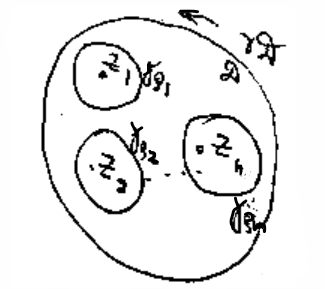
\includegraphics[width=2.8cm]{b41}
\end{wrapfigure}
$\blacklozenge$
$\quad$Построим окружности $\gamma_{\rho_k}=S(z_k;\rho_k)\subset D$
так, чтобы $B(z_k,\rho_k)$ не содержали других особых точек, кроме $z_k$.
На основании теоремы Коши для многосвязных областей:
\[
    \int_{\partial D}  f(z) \,dz =\sum_{k=1}^{n} \int_{\gamma_{\rho_k}}  f(z) \,dz=  \sum_{k=1}^{n}2\pi i \underset{\text{$z_k$}}{res f}= 2\pi i \sum_{k=1}^{n} \underset{\text{$z_k$}}{res f}
\]\begin{flushright}$\blacksquare$\end{flushright}


\textbf{Замечание 1.} \quad
Теорема справедлива и для неодносвязных областей, причём под $\partial D $ понимаем совокупность кривых, составляющих границу $D$, причём все кривые обходятся так, что область остается слева.

\textbf{Замечание 2.} \quad
Практическое значение теоремы состоит в том, что во многих случаях значительно проще вычислить вычет, чем интеграл, посему эта теорема может быть использована для вычисления интегралов ФКП.
\par\bigskip
\textbf{Теорема.} \quad 
\textit{Пусть f регулярна во всей расширенной плоскости комплексного переменного за исключением конечного числа изолированных особых точек.}
\textit{Тогда сумма вычетов функции, включая и вычет относительно бесконечно удаленной точки, равен нулю.
\[\sum_{k=1}^{n} \underset{\text{$z_k$}}{res f} + \underset{\text{$\infty$}}{res f}=0\]}\nextline
$\blacklozenge$\hspace{2 mm} Выберем R так, чтобы все конечные особые точки функции f лежали в круге B(0,R). \par\bigskip По основной теореме о вычетах \[
    \int_{S(0,R)}  f(z) \,dz = 2\pi i \sum_{k=1}^{n} \underset{\text{$z_k$}}{res f},
\]
$\quad$С другой стороны \[
    \int_{S(0,R)}  f(z) \,dz = -2\pi i  \underset{\infty}{res f},
\]
$\quad$Вычитая и получим требуемое.
\begin{flushright}$\blacksquare$\end{flushright}
\par\bigskip

\textbf{Следствие.} \quad
В условиях теоремы 
\[\underset{\text{$\infty$}}{res f}=-\sum_{k=1}^{n} \underset{\text{$z_k$}}{res f}\]
т.е. вычет функции $f$ относительно бесконечно удалённой точки равен сумме вычетов $f$, взятых с обратным знаком, относительно всех особых точек. Это обстоятельство используют при вычислении $\underset{\text{$\infty$}}{res f}$ и при вычислении интегралов.







\section{Вычисление интегралов вида $\displaystyle \int_0^{2\pi}R(\sin t, \cos t) dt$}
$R(u, v)$~--- рациональная функция своих переменных, причём предполагается, что на отрезке $[0, 2\pi]$ функция $R(\sin t, \cos t)$ не имеет особых точек. \\
Сделаем замену переменных, полагая $z = e^{it}$, то есть вводим комплексный аргумент.
Тогда 
\begin{gather*}
    \cos t = \frac{e^{it} + e^{-it}}{2} = \frac{z + \frac{1}{z}}{2} = \frac{z^2 + 1}{2z} \\
    \sin t = \frac{e^{iz} - e^{-iz}}{2i} = \frac{z - \frac{1}{z}}{2i} = \frac{z^2 - 1}{2iz} \\
    dz = ie^{it}dt \Rightarrow dt = \frac{dz}{iz}
\end{gather*}
\parИ в результате получим
\[ \int_0^{2\pi}R (\sin t, \cos t) dt = \frac{1}{i} \int_{|z| = 1} R \left(\frac{z^2 + 1}{2z}, \frac{z^2 - 1}{2iz} \right)\frac{dz}{z} \]
\par Подынтегральная функция является рациональной функцией $z$, значит, в круге $B(0,1)$ она голоморфна, за исключением, может быть, конечного числа изолированных особых точек, являющихся полюсами, либо УОТ.
Поэтому интеграл может быть вычислен с помощью теоремы о вычетах.

\begin{remark}
    Интеграл $\displaystyle \int_{-\pi}^{\pi} R(\sin t, \cos t) dt$ вычисляется по той же формуле.
    Указанным методом может быть вычислен и интеграл $\displaystyle \int_0^{\pi} R(\sin t, \cos t) dt = \frac{1}{2} \int_{-\pi}^{\pi} R(\sin t, \cos t) dt$
\end{remark}
\par\bigskip
\textbf{Пример.} \par\bigskip
$\displaystyle I = \int_0^\pi \frac{dt}{a + \cos t}, \quad |a| > 1$ \par\bigskip
$\displaystyle I = \frac{1}{2} \int_{-\pi}^{\pi} \frac{dt}{a + \cos t} = \frac{1}{2i} \int_{|z|=1} \frac{dz}{z \left( a + \frac{z^2 + 1}{2z} \right)} = \frac{1}{i} \int_{|z|=1} \frac{dz}{z^2+2az+1}$
$\displaystyle z_{1,2}=-a \pm \sqrt{a^2-1}$ \\
\begin{enumerate}
    \item $a > 1$. В круге $B(0,1)$ лежит корень $z_1 = -a+\sqrt{a^2-1}$, поэтому \\
        $\displaystyle I = \frac{1}{i}2\pi i \res_{z=z_1}{\frac{1}{z^2+2az+1}} = 2 \pi \frac{1}{2\left(-a+\sqrt{a^2-1}\right) +2a} = \frac{\pi}{\sqrt{a^2-1}}$
    \item $a<-1$. В круге $B(0,1)$ лежит корень $z_2 = -a-\sqrt{a^2-1}$ \\
        $\displaystyle I = \frac{2\pi}{2\left(-a-\sqrt{a^2-1}\right) +2a} = -\frac{\pi}{\sqrt{a^2-1}}$
\end{enumerate}
\par
\textit{Ответ}: $\displaystyle I = \frac{\pi \sgn a}{\sqrt{a^2-1}}$





\section{Вычисление интегралов вида $\displaystyle \int_{-\infty}^{+\infty}f(x) dx$}
Здесь будем рассматривать НИ-1, то есть предполагается, что $f(x)$ не имеет конечных особых точек на действительной оси.

Введем в рассмотрение функцию комплексного аргумента $f(z)$, которая совпадает с $f(x)$ при $z=x$ 
и предположим, что в верхней полуплоскости $f(z)$ имеет конечное число изолированных особых точек $z_1,\dotsc,z_n$.

\textbf{Лемма.} \quad
    \textit{Если существуют такие положительные постоянные} $R_0, M, \delta$\textit{,\\ что для всех точек верхней полуплоскости} $\ImR z>0$\textit{,
    удовлетворяющих условию} \\$\displaystyle |z|>R_0 \quad (z\in B(0, R_0, \infty)\;\cap\;\{z \;|\; \ImR z>0\})$ \textit{имеет место неравенство}
    $\displaystyle |f(z)| \leqslant \frac{M}{|z|^{1+\delta}}$, то
    \begin{equation} \label{lemma:1}
        \int_{C_\rho} f(z)dz \xrightarrow[\rho \to \infty]{} 0,
    \end{equation}
    \textit{где} $ C_\rho $~--- \textit{полуокружность} $|z|<\rho, \ImR z>0, \rho>R_0$

\blacklozenge 
    $\displaystyle \bigg\lvert\int_{C_\rho} f(z)dz \bigg\rvert \leqslant \int_{C_\rho} |f(z)||dz| \leqslant \int_{C_\rho} \frac{M}{\rho^{1+\delta}}|dz| = \frac{M}{\rho^{1+\delta}} \int_{C_\rho} |dz| = \frac{M}{\rho^{1+\delta}} \; \pi \rho = \frac{M\pi}{\rho^\delta} \xrightarrow[\rho \to \infty]{} 0 $
\blacksquare \par\bigskip
\textbf{Замечание 1.} \quad
Если условия леммы выполнены в секторе $\varphi_1<\arg z < \varphi_2$, то формула \eqref{lemma:1} имеет место, но в \eqref{lemma:1} $C_\rho$ - дуга окружности $S(0, \rho)$, лежащая в секторе.

\par\bigskip
\textbf{Замечание 2.} \quad
Условия леммы заведомо выполняются, если $z=\infty$ есть нуль порядка 2 или выше, а в окрестности $z=\infty$ функция регулярна.\\
\blacklozenge \hspace{3 mm} $\displaystyle f(z) = \frac{\psi(z)}{z^2}; \quad |\psi(z)|\leqslant M, \quad \delta=1$ \quad \blacksquare

В частности, если $f(z)$ рациональная функция $\displaystyle f(z)=\frac{P_n(z)}{Q_m(z)}$, $P_n, Q_m$~--- многочлены, то для выполнения леммы нужно потребовать $m>n+1$
\par\bigskip
\textbf{Теорема. } \quad
    \textit{Если функция} $f(z)$ \textit{не имеет особых точек на действительной оси и имеет лишь конечное число изолированных особых точек}
    $z_1, z_2, \dotsc, z_n$ \textit{в верхней полуплоскости, причём} $f(z)$ \textit{удовлетворяет условиям леммы} \eqref{lemma:1} \\\textit{и интеграл}
    $\displaystyle \int_{-\infty}^{+\infty}f(x)dx$ \textit{сходится, то}
    \begin{equation}
        \int_{-\infty}^{+\infty}f(x)dx = 2\pi i \sum_{k=1}^n \res_{z_k} f(z)
    \end{equation}


\begin{proof}
    $\blacklozenge$ Построим контур $C_R$, состоящий из полуокружности $\gamma_R$ в верхней полуплоскости и отрезка $[-R, R]$ действительной оси
    так, чтобы все особые точки попали в область ограниченную этим контуром. \\
    \begin{center}
        \begin{tikzpicture}
            \draw (0, 0) node[below]{$-R$} -- (3, 0) node[below]{$R$};
            \draw (3, 0) arc(0:180:1.5);
            \draw [->] (1,-0.1) -- (2,-0.1); 
        %   \draw (2,1) -- ++(30:2cm) (2,1) -- ++(60:2cm);
            \draw [->] ([shift=(80:1.5cm)]1.5,0.1) arc (80:100:1.5cm);
            \node[] at (0, 1.5) {$C_R$};
            \node[] at (3, 1) {$\gamma_R$};
            \node[circle, fill, inner sep=0.7pt] at (1, 0.3) {};
            \node[circle, fill, inner sep=0.7pt] at (2, 0.5) {};
            \node[circle, fill, inner sep=0.7pt] at (1.4, 1) {};
        \end{tikzpicture}
    \end{center}
    \par По основной теореме о вычетах
    $\displaystyle \int_{C_R} f(z)dz = 2\pi i \sum_{k=1}^n \res_{z_k} f(z)$ \par
    Но $\displaystyle \int_{C_R} f(z)dz = \int_{\gamma_R} f(z)dz + \int_{[-R, R]} f(z)dz$ \par\bigskip
    Перейдем к пределу при $R \to \infty$. Используя лемму, получим \\
    $$\displaystyle \int_{-\infty}^{+\infty}f(x)dx = 2\pi i \sum_{k=1}^n \res_{z_k} f(z)$$ \blacksquare
\end{proof}

\par\bigskip
\textbf{Следствие. } \quad
    Если $\displaystyle f(x)=\frac{P_n(x)}{Q_m(x)}$ и на оси нет особых точек, то для сходимости интеграла необходимо и достаточно, чтобы
    $\displaystyle \frac{P_n(x)}{Q_m(x)} \underset{x \to \infty}{\sim} \frac{A}{x^{m-n}} \quad \Rightarrow \quad m-n>1$ и тогда автоматически выполняются условия леммы, а, значит, и теоремы. \\
    Другими словами сходящийся НИ-1 от рациональной функции может быть всегда вычислен указанным методом.
    
\par\bigskip
\textbf{Замечание.} \quad
    Аналогично доказывается
    \begin{equation*}
        \int_{-\infty}^{+\infty} f(x)dx = -2\pi i \sum_{k=1}^n \res_{z_k} f(z),
    \end{equation*}
    где $z_k$ - особые точки функции $f(z)$ в нижней полуплоскости.

\par\bigskip
\textbf{Пример.}
    $\displaystyle I=\int_0^{+\infty} \frac{dx}{x^4+1}=\frac{1}{2}\int_{-\infty}^{+\infty} \frac{dx}{x^4+1}$ \\
    
    В силу следствия можно воспользоваться формулой теоремы. \par\bigskip
    Особые точки: $\displaystyle z_k=\sqrt[4]{-1} = e^{\frac{i\pi+2k\pi i}{4}} = e^{i \left(\frac{\pi}{4}+\frac{k\pi}{2}\right)}$ \par
    То есть: $z_1=e^{i {\pi \over 4}}, \quad z_2=e^{i \left(\frac{\pi}{4} + \frac{\pi}{2}\right)}, \quad
    z_3=e^{i \left(\frac{\pi}{4} + \pi\right)}, \quad z_4=e^{i \left(\frac{\pi}{4} + \frac{3\pi}{2}\right)}$ \par
    В верхней полуплоскости 2 особые точки: $z_1$ и $z_2$.\par\bigskip
    Поэтому $\displaystyle I={1 \over 2} \, 2\pi i \left(\res_{z_1} \frac{1}{z^4+1} + \res_{z_2} \frac{1}{z^4+1}\right) = 
    \pi i \left(\frac{1}{4z_1^3} + \frac{1}{4z_2^3}\right) = \pi i \left(\frac{z_1}{4z_1^4} + \frac{z_2}{4z_2^4}\right) = 
    -\frac{\pi i}{4} \left(z_1 + z_2\right) = -\frac{\pi i}{4} \left(\frac{\sqrt{2}}{2} + i\frac{\sqrt{2}}{2} - \frac{\sqrt{2}}{2} + i\frac{\sqrt{2}}{2}\right) = 
    -\frac{\pi i}{4} i \sqrt{2} = \frac{\pi \sqrt{2}}{4}$
    \par\bigskip
    Этот же интеграл можно вычислить по-другому. \\
    \begin{center}
        \begin{tikzpicture}
            \draw (0, 0) -- (3, 0);
            \draw (1, -1) -- (1, 2);
            \draw (3, 0) arc(0:90:2);
            \draw [->] (1.6,-0.1) -- (2.4,-0.1); 
            \draw [->] (0.9,1.4) -- (0.9, 0.6); 
            \draw [->] ([shift=(30:2.1cm)]1,0) arc (30:60:2.1cm);
            \node[] at (0, 1.5) {$C_R$};
            \node[] at (3.2, 0.9) {$\gamma_R$};
        \end{tikzpicture}
    \end{center}
    \par
    $\displaystyle \int_{\gamma_R} \to 0$ по лемме. \par
    $\displaystyle \int_{C_R} = \int_{\gamma_R} + \int_0^R \frac{dx}{1+x^4} - \int_0^{iR} \frac{dz}{1+z^4} = 
    2 \pi i \res_{z_1} \frac{1}{1+z^4} = 2\pi i \, \frac{z_1}{4z_1^4} = -\frac{2\pi i}{4} \left(\frac{\sqrt 2}{2} + i \, \frac{\sqrt 2}{2}\right)$ \par
    $\displaystyle \int_0^{iR} \frac{dz}{1+z^4} = \left[x=0, y=y \quad z=iy\right] = \int_0^{iR} \frac{idy}{1+y^4};$ \par\bigskip
    Перейдя к пределу \par
    $\displaystyle I-iI = -\frac{\pi i}{2} \left(\frac{\sqrt 2}{2} + i \, \frac{\sqrt 2}{2}\right) \quad \Rightarrow \quad I=\frac{\pi\sqrt 2}{4}$






\section{Интегралы вида $\int\limits_{-\infty}^{+\infty}e^{i\alpha x} f(x)\, dx$, лемма Жордана}
\par \textbf{Лемма 1.} $\ sin\,x \ge \frac{2}{\pi}x, \quad x \in [0, \frac{\pi}{2}]\\ $ 
\bigskip
\begin{wrapfigure}[4]{l}{0.3\linewidth} 
    \vspace{-6ex}
    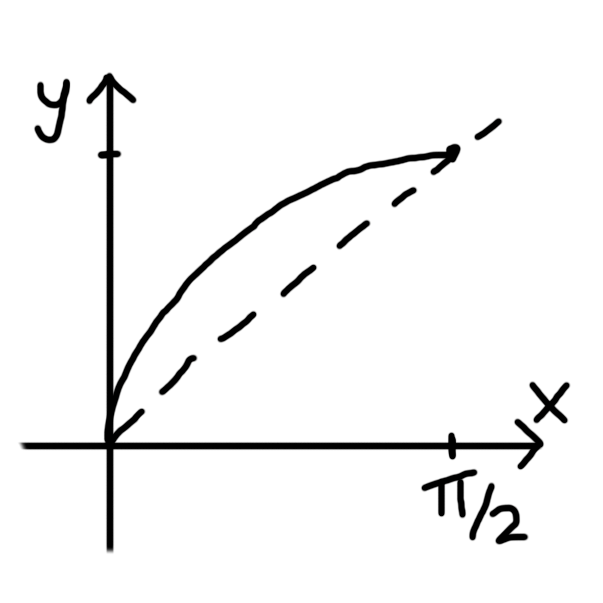
\includegraphics{jordan/1int.png}
\end{wrapfigure}
$\blacklozenge$ Функция $sin$ выпукла вверх на $[0, \frac{\pi}{2}]$, поэтому её график лежит выше хорды, соединяющей её концы.
\\ уравнение хорды \quad $y = \frac{2}{\pi}x$ \quad $=>$
\\ $sin\,x \ge \frac{2}{\pi}x$, \quad $\forall x \in [0, \frac{\pi}{2}]$ \ 
$\blacksquare$
\bigskip\bigskip\bigskip\par
\textbf{Лемма Жордана.}\quad \textit{Пусть} $f(z)$ \textit{регулярна в верхней полуплоскости} $Im\,z \ge 0$ \textit{за исключением конечного числа изолированных особых точек, и }
$\smash{\displaystyle\max_{\gamma_{R}}} |f(z)| \rightarrow_{R \rightarrow \infty} 0$, \textit{где} $\gamma_R ::= S(0, R) \cap {\{z|Im\,z \ge 0}\}$.
\bigskip \\  \textit{Тогда, при} $fix\,\alpha > 0$ \quad $\Rightarrow \quad \lim\limits_{R \rightarrow \infty} \int\limits_{\gamma_{R}} f(z)e^{i\alpha z}\, dz = 0$ 
\bigskip \\
$\blacklozenge \hspace{1 mm}$ Т.к. $\smash{\displaystyle\max_{\gamma_{R}}} |f(z)| \rightarrow 0$ при $R \rightarrow \infty$ \quad $\Rightarrow$ \ 
$\forall \epsilon > 0,\ \exists R_0(\epsilon), \ \forall z \in \gamma_{R_0} \Rightarrow |f(z)| \le \epsilon$ \par\bigskip
Рассмотрим 
\begin{center}
    $\int\limits_{\gamma_{R}} e^{i\alpha z}f(z)\, dz = \begin{bmatrix} z = Re^{i\varphi} \\ 0 \le \varphi \le \pi \end{bmatrix} = \int\limits_{0}^{\pi} e^{i \alpha\varphi R e^{i\varphi}}f(R e^{i\varphi}) R i e^{i\varphi}\, d\varphi$
\end{center}
\par Возьмём $R > R_0$. Тогда 
\begin{center}
    $|\int\limits_{\gamma_{R}} e^{i\alpha z}f(z)\, dz|\ \le\  R\int\limits_{0}^{\pi} |e^{i \alpha\varphi R (cos\,\varphi + i sin\,\varphi)}|\cdot|f(R e^{i\varphi})|\, d\varphi\  \le\ R\int\limits_{0}^{\pi} e^{- \alpha R sin\,\varphi}\cdot \epsilon\, d\varphi\ =\ 2R\epsilon \int\limits_{0}^{\frac{\pi}{2}} e^{- \alpha R sin\,\varphi}\, d\varphi\ \le\ $\par[по лемме 1]$\ \le
    \ 2R\epsilon \int\limits_{0}^{\frac{\pi}{2}} e^{- \alpha\varphi R \frac{2}{\pi}\varphi}\, d\varphi\ =\ -\frac{2R\varphi\pi}{2R\alpha} e^{-\alpha R \frac{2}{\pi} \varphi}\ \bigg|_{0}^{\frac{\pi}{2}}\ =\ \frac{\pi \epsilon}{\alpha} (1 - e^{-\alpha R})\ \le\ \frac{\pi}{\alpha}\epsilon
    \quad \blacksquare$
\end{center}
\par\bigskip
\textbf{Замечание.}\ Если $\alpha < 0$, а $f$ удовлетворяет условию леммы Жордана в некоторой полуплоскости, то заключение леммы имеет место по дуге окружности в нижней полуплоскости:
\begin{center}
    $\lim\limits_{R \rightarrow \infty} \int\limits_{\gamma_{R}} e^{-i\beta z}f(z)\, dz, \quad \beta > 0$
\end{center}
\par Аналогичное утверждение имеет место для правой полуплоскости:
\begin{center}
    $\lim\limits_{R \rightarrow \infty} \int\limits_{\gamma_{R}} e^{-\beta z}f(z)\, dz, \quad \beta > 0$
\end{center}
\par для левой полуплоскости:
\begin{center}
    $\lim\limits_{R \rightarrow \infty} \int\limits_{\gamma_{R}} e^{\beta z}f(z)\, dz, \quad \beta > 0$
\end{center}

\textbf{Теорема.} \ \textit{Пусть} $f(z)$:
\begin{enumerate} 
\item \textit{регульярна в верхней полуплоскости за исключением конечного числа изолированных точек} $z_1, z_2, \dots, z_n$
\item \textit{не имеет особых точек на действительной оси}
\item $|f(z)| \rightarrow 0$ \textit{при} $z \rightarrow \infty$,\quad $Im\,z \ge 0$
\end{enumerate}
\par \textit{Тогда при} $\alpha > 0$
\begin{center}
    $\int\limits_{-\infty}^{+\infty}e^{i\alpha x} f(x)\, dx = 2\pi i \sum\limits_{-\infty}^{\infty} \overset{}{\underset{z_k}{res}} (f(z) e^{i\alpha z})$
\end{center} 
\begin{wrapfigure}[4]{r}{0.2\linewidth} 
    \vspace{-10ex}
    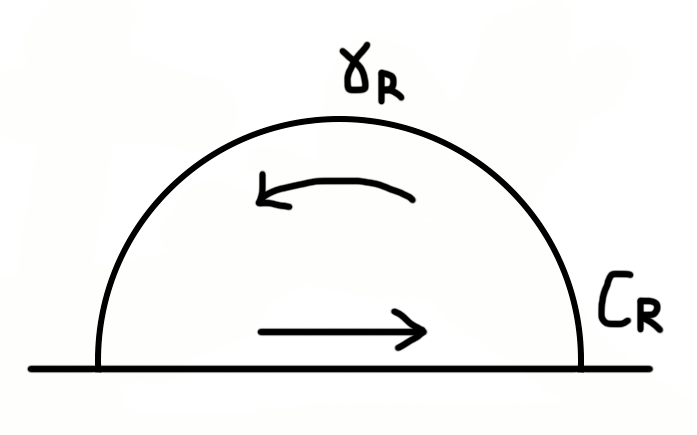
\includegraphics{jordan/2_2.png}
\end{wrapfigure}
\\
$\blacklozenge \hspace{1 mm} \int\limits_{C_R} = \int\limits_{\gamma_R} + \int\limits_{-R}^{R} = 2\pi i \sum\limits_{k=1}^{n} \overset{}{\underset{z_k}{res}}\,f(z) e^{i\alpha z}$ 
\par\bigskip Переходя к пределу и используя при этом лемму Жордана, получаем требуемое.$\blacksquare$
\par\bigskip
\textbf{Замечание 1.} \quad Для $\alpha < 0,\ \alpha = -\beta,\ \beta > 0$ с учётом леммы Жордана имеем:
\begin{center}
    $\int\limits_{-\infty}^{+\infty}e^{-i\beta x} f(x)\, dx = -2\pi i \sum\limits_{k=1}^{n} \overset{}{\underset{z_k}{res}}\,f(z) e^{-i\beta z}$
\end{center}
\par где $z_k$ --- особоая точка в нижней полуплоскости.
\par\bigskip
\textbf{Замечание 2.} \quad Теорема даёт возможность вычислять интегралы вида
\begin{center}
    $\int\limits_{-\infty}^{+\infty} f(x) cos\,x\, dx = Re\int\limits_{-\infty}^{+\infty}e^{i\alpha x} f(x)\, dx$
    \par
    $\int\limits_{-\infty}^{+\infty} f(x) sin\,x\, dx = Im\int\limits_{-\infty}^{+\infty}e^{i\alpha x} f(x)\, dx$
\end{center}

\textbf{Пример.} \quad Вычислить интегралы Лапласа
\begin{center}
    $I_1 = \int\limits_{0}^{+\infty} \frac{cos\,\alpha x}{x^2 + a^2}\, dx, \quad I_2 = \int\limits_{0}^{+\infty} \frac{x\, sin\,\alpha x}{x^2 + a^2}\, dx, \quad a > 0, \alpha > 0$
\end{center}
\par
$I_1 = \frac{1}{2}\int\limits_{-\infty}^{+\infty} \frac{cos\,\alpha x}{x^2 + a^2}\, dx, = \frac{1}{2}Re\int\limits_{-\infty}^{+\infty}\frac{e^{i\alpha x}}{x^2 + a^2} \, dx = \frac{1}{2} Re(2\pi i\; \overset{}{\underset{ia}{res}} \frac{e^{i\alpha z}}{z^2 + a^2}) = \frac{1}{2} Re(2\pi i\; \frac{e^{-\alpha a}}{2ai}) = \frac{\pi}{2a} e^{-\alpha a}$
\par\bigskip Аналогично
\par\bigskip
$I_2 = \frac{1}{2}Im\int\limits_{-\infty}^{+\infty}\frac{x\; e^{i\alpha x}}{x^2 + a^2} \, dx = \frac{1}{2} Im(2\pi i\; \overset{}{\underset{ia}{res}} \frac{z\;e^{i\alpha z}}{z^2 + a^2}) = \frac{1}{2} Im(2\pi i\; \frac{ai\; e^{-\alpha a}}{2ai}) = \frac{\pi}{2} e^{-\alpha a}$






\section{$v.p.  \int\limits_{-\infty}^{\infty} e^{i\alpha x} f(x) \, dx, \alpha>0.$}

Пусть $f(z)$:
\begin{enumerate}
    \item Голоморфна в верхней полуплоскости, за исключением конечного числа изолированных особых точек $z_1\dots,z_n$
    \item Имеет на оси $Ox$ простые полюса $x_1,\dots,x_m$
    \item $|f(z)|\rightarrow 0, z \rightarrow 0, z\geq 0$
\end{enumerate}

При этих условиях интеграл  $\int\limits_{-\infty}^{\infty} e^{i\alpha x} f(x) \, dx$  расходится, но может существовать в смысле главного значения.
\par\bigskip

\begin{wrapfigure}[4]{l}{0.4\linewidth} 
    \vspace{-6ex}
    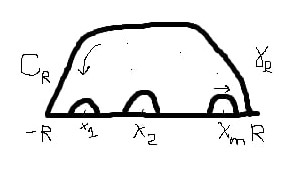
\includegraphics{v.p. e/1.jpg}
\end{wrapfigure}
Построим $C_R$ так, чтобы все особые точки попали в область им ограниченную, а $r_{k\rho}$ не имели общих точек.
Другими словами, $C_R$ контур изображений на рисунке.
\par\bigskip\bigskip
Тогда: $$\int\limits_{C_r} f(z)e^{i\alpha z} dz = \int\limits_{\gamma_R} + \int\limits_{-R}^{x_1-\rho}+\int\limits_{-R}^{x_2-\rho}+\dots+\int\limits_{x_m+\rho}^{R}+\sum\limits_{k=1}^{m}\gamma_{k\rho}= 2\pi i\sum\limits_{k=1}^{u}res e^{i\alpha z}f(z)$$
\par\bigskip
Рассмотрим каждый интеграл в отдельности в левой части этого равенства.
\par\bigskip
$\int\limits_{\gamma_R}\underset{R \to \infty}{\to}0$ в силу леммы Жордана
\par\bigskip
$$\int\limits_{-R_1}^{x_1-\rho}+\dots+\int\limits_{x_m+\rho}^{R}\underset{R \to \infty;\rho \to \infty}{\longrightarrow}  v.p.\int\limits_{-\infty}^{+\infty}f(x) e^{i\alpha x} d(x)$$
\par\bigskip
$\int\limits_{\gamma_{k\rho}} f(z) e^{i\alpha z}dz=\int\limits_{\gamma_{k\rho}}(\frac{C_{-1}^{(k)}}{z-x_k}+C_0^{(k)}+C_1^{(k)}(z-x_k)+\dots)dz=|\int\limits_{\gamma_{k\rho}}(z-x_k)^n dz=|z=x_k+\rho e^{i\phi}|=\int\limits_{\pi}^{0} \rho^n e^{i\phi}i d\phi = -i\rho^{n+1}\int\limits_{0}{\pi}e^{i(n+1)\phi}d\phi\rightarrow 0 $\quad для $\forall n \geqslant 0.$
\par\bigskip
$\int\limits_{\rho_{kg}}\dfrac{dz}{z-x_k}= - \int\limits_{0}{\pi}\dfrac{\rho e^{i\phi}i}{\rho e^{i\phi}}d\phi=-\pi i.$
\par\bigskip
Поэтому, $$\int\limits{\gamma_{kg}} f(z)e^{i\alpha z}dz=-\pi i C_{-1}^{(k)}= -\pi \underset{z=x_k} {res} f(z)e^{idz}$$
\par\bigskip
Переходя к пределу при $R\rightarrow\infty, g\rightarrow 0$ окончательно получаем:
$$v.p. \int\limits_{-\infty}^{\infty}f(z)e^{i \alpha x} dx= 2\pi i \sum\limits{k=1}{n}\underset{z_k}{res} e^{i\alpha z}f+\pi\sum\limits{1}{m}\underset{x_k}{res}fe^{i\alpha x}$$


  \textbf{Примеры:} 
\begin{enumerate}
    \item Интеграл Дирихле $\beta >0$\par
$$\int\limits_{0}^{+\infty}\dfrac{sin\beta x}{x}dx=\dfrac{1}{2}\int\limits_{-\infty}^{+\infty}\dfrac{sin\beta x}{x}dx=\dfrac{1}{2}Im\int\limits_{-\infty}^{\infty}\dfrac{e^{i\beta x}}{x}dx=\dfrac{1}{2}Im\: \pi \:i\: \underset{z=0}{res}\: \dfrac{e^{i\beta z}}{z}=\dfrac{\pi}{2}$$

\item Интеграл Френеля

$$I_1= \int\limits_{0}^{+\infty} cosx^2dx,\: I_2= \int\limits_{0}^{+\infty} sinx^2dx$$

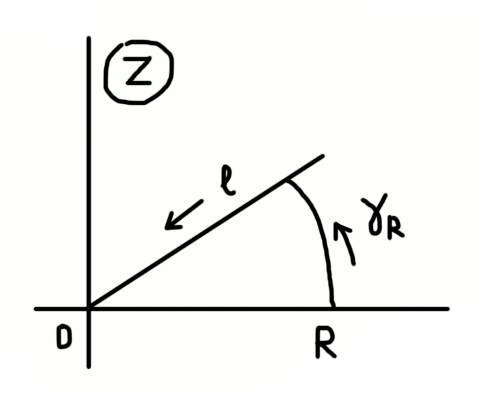
\includegraphics[width=6 cm]{frenel.png}

Рассмотрим $\int\limits_{C_R}e^{i z^2}dx=\int\limits_{0}^{R}e^{i x^2}dx+\int\limits_{\gamma_R}e^{i z^2}dz+\int\limits_{e}e^{i z^2}dz=0$

1)\quad $\int\limits_{0}^{R}e^{i x^2}dx\underset{R\rightarrow\infty}{\longrightarrow}\int\limits_{0}^{+\infty}e^{i x^2}dx$

2)\quad $\int\limits_{\gamma_R}e^{i z^2}dz = |z=Re^{i\phi}|=\int\limits_{0}^{\dfrac{\pi}{4}}e^{iR^2e^{2i\phi}}R\: i\: e^{i\phi}d\phi=>|\int\limits_{\gamma_R}e^{i z^2}dz|\leqslant R \int\limits_{0}^{\dfrac{\pi}{4}}e^{-R^2sin2\phi}d\phi\leqslant R\int\limits_{0}^{\dfrac{\pi}{4}}e^{-R^2\dfrac{\pi}{4}\phi}d\phi=-R\dfrac{\pi}{4R^2}e^{-R^2\dfrac{4}{\pi}\phi}\bigg|_0^{\dfrac{\pi}{4}}=\dfrac{\pi}{4R}(1-e^{R^2}\rightarrow 0),$ при $R\rightarrow 0$.

3) \quad $\int\limits_{e}e^{iz^2}dz=|\underset{0\leqslant	t\leqslant	R}{z=te^{i\dfrac{\pi}{4}}}|=-\int\limits_{0}^{R}e^{it^2e^{i\dfrac{\pi}{2}}e^{i\dfrac{\pi}{4}}}dt= - e^{i\dfrac{\pi}{4}}\int\limits_{0}^{R}e^{-t^2}dt\underset{R\rightarrow\infty}{\longrightarrow}-e^{i\dfrac{\pi}{4}}\dfrac{\sqrt{\pi}}{2}$

Переходя к пределу, получим:

$$\int\limits_{0}^{+\infty}e^{ix^2}dx-\dfrac{\sqrt{\pi}}{2}e^{i\dfrac{\pi}{4}}=0 \Rightarrow\int\limits_{0}^{+\infty}e^{ix^2}dx=\dfrac{\sqrt{\pi}}{2}e^{i\dfrac{\pi}{4}}.$$
\parОтделяя действительную и мнимую части, получим:
$$\int\limits_{0}^{+\infty}cosx^2dx=\int\limits_{0}^{+\infty}sinx^2dx=\dfrac{1}{2}\sqrt{\dfrac{\pi}{2}}$$

\end{enumerate}



\section{Логарифмический вычет}

Пусть в области $D$ задана функция $f$ регулярная за исключением конечного числа изолированных особых точек, являющихся полюсами $a_1,a_2,\dots,a_\phi.$ Составим функцию $lnf(z).$ \par Функцию $\phi(z)::=(ln f(z))'= \dfrac{f'(z)}{f(z)}$ назовем \textbf{логарифмической производной функции $f$}. Вычеты функции $\phi(z)=\dfrac{f'(z)}{f(z)}$ относительно ее особых точек будем называть \textbf{логарифмическими вычетами $f$}. \par\bigskip Какие же точки могут быть особыми для $\phi$? Нетрудно видеть, что таковыми будут нули и полюса функции $f$. Других особых точек быть не может. Исследуем эти точки:
\begin{enumerate}
    \item Пусть точка $z=b\in D$ является нулем кратности $n$ для функции $f$. Тогда $f$ в некоторой окрестности точки $b$, т.е. в $b(b,0,\zeta)$ можно представить в виде $$f(z)=(z-b)^ng(z)$$ где $g$-голоморфна в $z=b$ и $g(b)\ne 0.$ \parТогда $g(z)\ne 0$ и в некоторой окрестности точки $b$ (нам известно, что нули голоморфной функции изолированы). Поэтому, в $B(b,0,\zeta)$ $$lnf(z)=n ln(z-b)+ln g(z)$$  $$\phi(z)=\dfrac{f'(z)}{f(z)}=\dfrac{n}{z-b}+\dfrac{g'(z)}{g(z)},$$ где $\dfrac{g'(z)}{g(z)}$ регулярна в $B(b,0,\zeta)$ и ее разложение в ряд Лорана в окрестности точки $b$ не будет содержать главной части. Тогда $$ \dfrac{f'(z)}{f(z)}=\dfrac{n}{z-b}+ C_0 + C_1(z-b)+C_2(z-b)^2+\dots$$ Отсюда следует, что $$\underset{z=b}{res}\dfrac{f'(z)}{f(z)}=n$$ т.е. в нуле кратности $n$ логарифмическая производная голоморфной функции $f$ имеет полюс первого порядка и логарифмический вычет $f$ равен кратности нуля.
    
    \item Пусть $z=a$ - полюс порядка $p$ функции $f$, тогда $$f(z)=\dfrac{\psi(z)}{(z-a)^p}$$ $\psi(z)$ регулярна в а и $\psi(a)\ne 0\Rightarrow \psi(a)\ne 0$ и в некоторой окрестности точки а.

$$ln f(z) = - p\,ln(z-a)+ln\psi(z)$$
$$\dfrac{f'(z)}{f(z)}= \dfrac{-p}{z-a}+\dfrac{\psi'(z)}{\psi(z)}\quad \Rightarrow \quad \underset{a}{res}\dfrac{f'(z)}{f(z)}=-p.$$

Таким образом, в полюсе порядка p логарифмическая производная функции $f$ имеет простой полюс и логарифмический вычет в этом полюсе равен порядку полюса с обратным знаком.
\end{enumerate}





\section{Принцип аргумента }
\\В дальнейшем, если не оговорено противное, условимся каждый нуль и полюс считать столько раз, каков его порядок и употреблять в этом случае выражения "полное число нулей" и "полное число полюсов".
\par\bigskip
\textbf{Теорема.} \quad
\textit{Пусть \(f\) голоморфна в односвязной замкнутой области \(D\) за исключением конечного числа полюсов \(a_1, a_2, ... a_k\) порядков \(p_1, p_2, ... p_k\) собственно. Пусть \(b_1, b_2, ... b_m\) - нули функции \(f\), порядки которых \(n_1, n_2, ... n_m\) соответственно. 
\\Если \(f\) не имеет ни нулей, ни полюсов на границе \(\delta D\) области \(D\), то 
\( \frac{1}{2\pi} \int\limits_{\delta D}  \frac{f'(z)}{f(z)} dz = N-P\)
\\ где \( N = \sum\limits_{j=1}^{m} n_j \) - полное число нулей, а \( P= \sum\limits_{j=1}^{k} p_j\) - полное число полюсов, а \(\delta D\) обходится в положительном направлении.}\\
\bigskip
\\$\blacklozenge$ \hspace{1 mm} Интеграл теоремы может быть вычислен с помощью основной теоремы о вычетах $$ \frac{1}{2\pi} \int\limits_{\delta D}  \frac{f'(z)}{f(z)} dz = \sum\limits_{k} res_{z_k} \frac{f'(z)}{f(z)}  $$ где \(z_k\) --- особые точки подинтегральной функции. Учитывая результаты исследования предыдущего пункта, имеем  $$ \frac{1}{2\pi} \int\limits_{\delta D}  \frac{f'(z)}{f(z)} dz = n_1 + n_2 + ... + n_m - p_1 - p_2 - ... - p_k = N-P$$  $\blacksquare $  

\par\bigskip
\textbf{Замечание.} \quad Теорема имеет место и для неодносвязной области. 

\par\bigskip Доказанной теореме можно дать удобную геометрическую трактовку.
\par Представим \( f(z) = R e^{i\Phi}\), где \(R=|f(z)|\) , \(\Phi = \arg f(z)\) тогда  \(\ln f(z) = \ln R + i\Phi\)  
\\Поэтому \( d\ln f(z) = \frac{f'(z)}{f(z)} dz = d\ln R + id\Phi \) и , следовательно
$$ \frac{1}{2\pi} \int\limits_{\delta D}  \frac{f'(z)}{f(z)} dz = \frac{1}{2\pi} \int\limits_{\delta D} d\ln R + \frac{1}{2\pi} \int\limits_{\delta D}  d\Phi = N-P$$
\par\bigskip
\\Рассмотрим каждый из интегралов в отдельности 
\begin{wrapfigure}[8]{l}{0.4\linewidth} 
    \vspace{-1ex}
    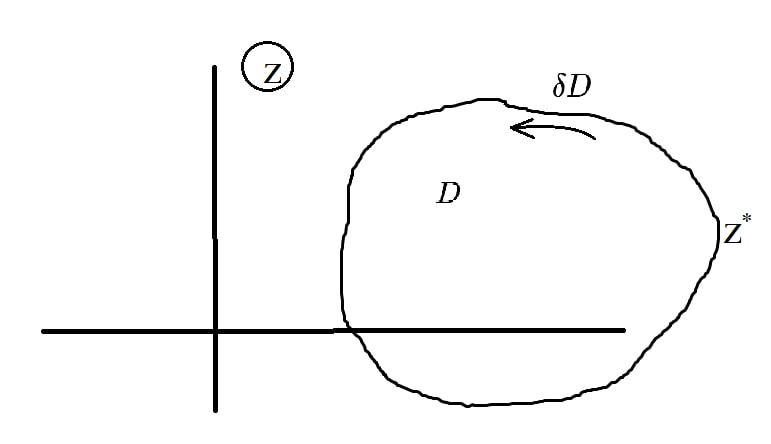
\includegraphics[width=6 cm]{argument/1.jpg}
\end{wrapfigure}
\\Выберем на  \(\delta D\) произвольным образом точку \(z^+\), каждую будем считать начальной точкой при интегрировании. Она же будет и конечной.

\\Функция \(f\) на  \(\delta D\) регулярна, а значит, однозначна. Она не имеет на  \(\delta D\) ни нулей, ни полюсов. Следовательно, однозначной будет и функция \(\ln R = \ln |f(z)|\), так как это уже взята главная ветвь логарифма - однознаяная функция.\par\bigskip \(ln|f(z)|\) - непрерывна на контуре  \(\delta D\) в силу указанных выше обстоятельств. В силу непрерывности \(\int\limits_{\delta D} dln|f(z)|\) можно вычислить по формуле Ньютона-Лейбница, а в силу однозначности, при обходе контура \(\delta D\) точкой \(z\) функция \(ln|f(z)|\) возвращается к первоначальному значению.\par Таким образом, получаем: 
$$\int\limits_{\delta D} d\ln R = \int\limits_{\delta D}  d\ln|f(z)| = \ln|f(z)|\bigg|_{z^*}^{z^*}=0 $$
\parВеличина же  \(\Phi = \arg f(z)\)  может при обходе контура \(\delta D\) измениться. Обозначим изменение аргумента при обходе контура \(\delta D\) через 
\( \Delta_{\delta D} \arg f(z) \)   
\parтогда $$\int\limits_{\delta D} d\phi = \int\limits_{\delta D} d \arg f(z) = \phi _1 - \phi_2 = \Delta_{\delta D} \arg f(z).$$
\par И тогла равенство из теоремы можно записать в следующем виде 
\begin{center}
    \fbox{\(N-P= \frac{1}{2\pi}  \Delta_{\delta D} \arg f(z)\)}
\end{center}
 
\\Это равенство и называют принципом аргумента.
\par\bigskip
В условиях теоремы разность между полным числом нулей и полным  числом полюсов функции \(f\) в области \(D\) равна деленому на \(2\pi\) изменению аргумента этой функции при обходе точкой \(z\) граница области \(\delta D\) в положительном направлении.
\par\bigskip
\textbf{Замечание.} \quad
Принцип аргумента имеет место и в случае, когда \(f(z)\)  голоморфна в \(D\) за исключением конечного числа полюсов и непрерывна в \(\overline{D}\).
\\
\par Изучим геометрический смысл принципа аргумента.
\begin{figure}[bh]
\begin{minipage}[t]{0.5\linewidth}
\center{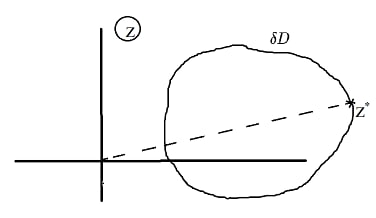
\includegraphics[width=0.6\linewidth]{argument/2.jpg}
\end{minipage}
\hfill
\begin{minipage}[t]{0.5\linewidth}
\center{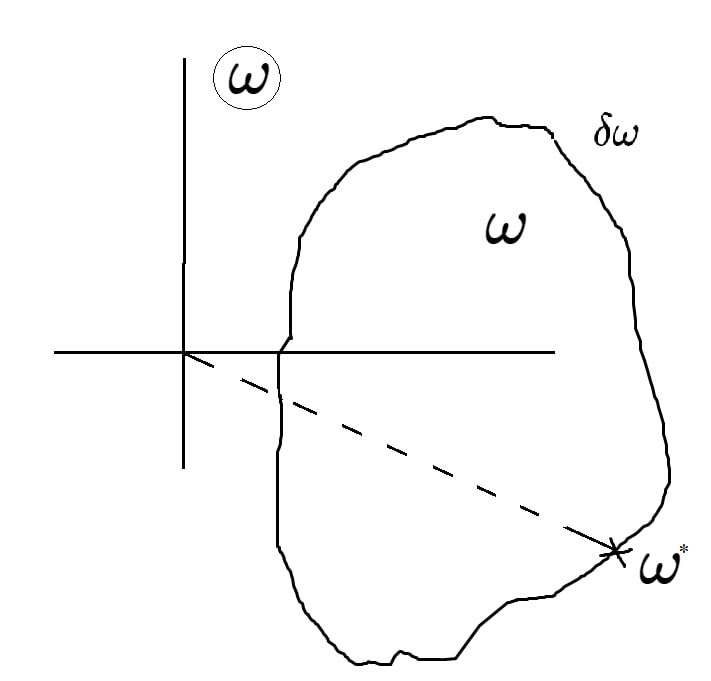
\includegraphics[width=0.6\linewidth]{argument/3.jpg}}
\end{minipage}
\hfill
\end{figure}
\\\parТ.к. \(f\) непрерывна в \(\overline{D}\), то образом области \(D\) при отображении \(\omega = f(z)\) является некоторая область ХЗ в плоскости \(\omega\). При этом \(\delta D \rightarrow \delta\omega \).

\par\bigskip При этом возможны два случая:
\begin{enumerate}
    \item точка \(\omega = 0 \not\in \omega  \) Проследим в этом случае за изменением \(\arg f(z) = \arg \omega \). Это изменение определяется числом полных оборотов вектора \(o\omega\) при полном обходе точкой \(z\) контура \(\delta D \). Нетрудно видеть, что в этом случае \(\Delta_{\delta D} \arg f(z) = \Delta_{\delta D} \arg \omega = 0\), то есть \(N=P\).
\\Если известно о \(f\) чуть больше, скажем, что она голоморфна в \(D\), то сразу же следует, что и нулей у неё в этом случае в \(D\) нет.

\item точка \(\omega = 0 \in D  \)
\par\\Тогда \( \frac{1}{2\pi}  \Delta_{\delta D} \arg f(z) = \frac{1}{2\pi}  \Delta_{\delta D} \arg \omega \) даёт полное число обротов, которое совершает вектор \( o\omega\) при обходе контура \(d\omega\), то есть \(N-P\) показывает изменение  \( \frac{1}{2\pi}  \Delta_{\delta D} \arg f(z) \)

\end{enumerate}
\begin{wrapfigure}[3]{l}{0.3\linewidth} 
    \vspace{-6ex}
    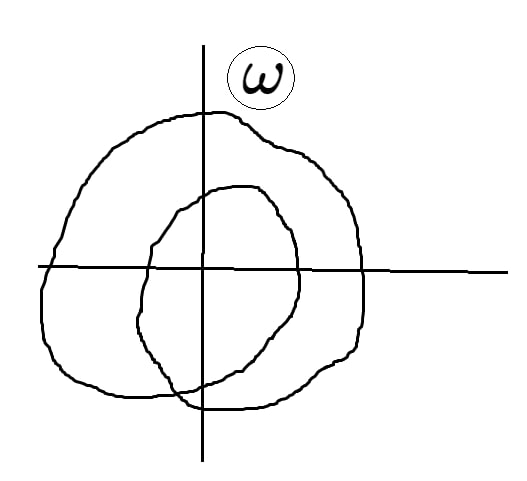
\includegraphics[width=3 cm]{argument/4.jpg}
\end{wrapfigure}

\\ Движение может быть как в положительном, так и в отрицательном направлении. Это зависит от свойст \(f\). На рисунке \(N-P=2\)

\nextline
\par\bigskip
\section{Теоема Руше }
Соображения, восказанные в предыдущем пункте, часто оказывается удобными при подсчёте полного числа нулей функции \(f\) регулярной в заданной области, на основании вышеизложенного, если \(f\) голоморфна в \(\overline{D}\),  то $$N= \frac{1}{2\pi}  \Delta_{\delta D} \arg f(z)$$ 
\\ Oднако во многих случаях вычисления можно упростить, используя следующую теорему:
\par\bigskip
\textbf{Теорема Руше.}
\quad
\textit{Пусть функция \(f\)  и \(g\) регулярны в замкнутой ограниченной области \(\overline{D}\), причём на границе  \(\delta D \) этой области  выполняется \( |f(z)|>|g(z)|\). 
\\ Тогда полное число нулей функции \(f\) в области \(D\) равно полному числу нулей функции \(f+g\) в этой области}
\bigskip\\
$\blacklozenge$  \hspace{1 mm} Так как  \( |f(z)|>|g(z)| \geq 0 \quad \Rightarrow \quad f(z)\) не обращается в 0 на    \(\delta D \).
\par\bigskip Так как  \( |f(z) + g(z)| \geq |f(z)| - |g(z)| > 0 \quad \Rightarrow \quad f+g\) не обращается в 0 на    \(\delta D \).
\par\bigskip Применим к \(f\) принцип аргумента 
$$ N_f =  \frac{1}{2\pi}  \Delta_{\delta D} \arg f(z) $$
\par Сделаем то же для  функции \(f+g\)

\( N_{f+g} =  \frac{1}{2\pi}  \Delta_{\delta D} \arg (f(z) + g(z)) =  \frac{1}{2\pi}  \Delta_{\delta D} \arg f(z)(1 + \frac{g(z)}{f(z)} ) = \frac{1}{2\pi}  \Delta_{\delta D} \arg f(z) + \frac{1}{2\pi}  \Delta_{\delta D} \arg (1 + \frac{g(z)}{f(z)} ) = N_f + \frac{1}{2\pi}  \Delta_{\delta D} \arg (1 + \frac{g(z)}{f(z)} )\) 
\par\bigskip Теперь осталось показать, что последнее слагаемое равно 0. Для этого рассмотрим функцию $$\omega = 1 + \frac{g(z)}{f(z)} $$
$$\omega - 1 =  \frac{g(z)}{f(z)} \quad \Rightarrow \quad |\omega - 1 | =  \frac{|g(z)|}{|f(z)|} < 1$$
\par то есть \(|\omega - 1| < 1\).
\par\bigskip Это неравенство говорит о том, что приобходе точкой \(z\) контура  \(\delta D \) точка \(\omega = 1 + \frac{g(z)}{f(z)} \) описывает замкнутую кривую \(\delta G\), целиком лежащую в круге \(B(1,1)\), то есть контур \(\) не охватывает точку \(\omega = 0\), то есть  \(\omega = 0 \not\in G  \). Тогда на основании принципа аргумента $$\Delta_{\delta D} \arg (1 + \frac{g(z)}{f(z)})=0 $$\par\bigskip окончательно \(N_f = N_{f+g}\)  $\blacksquare $  





\section{Следствие: Основная теорема алгебры}

\hangindent=11pt \hangafter=0 \noindent \textbf{Теорема}

\hangindent=11pt \hangafter=0 \noindent \textit{Всякий многочлен $P_n(z) = C_n z^n + C_{n-1} z^{n-1} + \cdots + az + C_0, \ C_n \not= 0$, степени n с комплексными коэффициентами имеет в компактной плоскости ровно n косплексных корней.}
\par\bigskip

\begin{Proof}
Представим $P_n(z)$ в виде $P_n(z) = f(z) + g(z)$, положив $f(z) = C_n z^n, \ g(z) = C_{n-1} z^{n-1} + \cdots C_0$. Так как $\frac{g(z)}{f(z)} = \frac{C_{n-1}}{C_n} \cdot \frac{1}{z} + \cdots + \frac{C_0}{C_n} \cdot \frac{1}{z^n} \longrightarrow_{z\rightarrow \infty} 0$, то $\exists R_0$ такое, что $\forall z, \ |z|\geqslant R_0 \Rightarrow \left| \frac{g(z)}{f(z)} \right| \leqslant 1$. Возьмём некоторое $R > R_0$. Тогда для $\forall z \in S(0, R) \Rightarrow \left| \frac{g(z)}{f(z)} \right| < 1 \Rightarrow |f(z)| > |g(z)|$

На основании теоремы Руше $N_{P_n} = N_f$. Но $f = a_n z_n$ имеет в круге $B(0, R)$ n нулей, поэтому полное число нулей функции $f+g = P_n(z)$ также равно и в круге $B(0,R)$, а вне круга $P_n(Z)$ не может иметь нулей в силе неравенства $\left| \frac{g(z)}{f(z)} \right| < 1$.
\end{Proof}
\par\bigskip

\textbf{Пример 1.} \quad
Найти число нулей функции $F(z) = z^8 - 4z^5 + z^2 - 1$ в круге $B(0,1)$.
$f = -4z^5; \ g = z^8 + z^2 -1; \ $ на $S(0,1): \ |f(z)| = 4, \ g(z) \leqslant 3 \Rightarrow |f| > |g|$. Так как $N_f = 5 \Rightarrow N_F = 5$.
\par\bigskip

\textbf{Пример 2.} \quad
$F(z) = z^8 + 6z + 10$ в $B(0,1)$
$$f = 10,\ g = z^8 + 6z; \ |f| = 10,\ |g| \leqslant 7 \Rightarrow N_F = 0.$$
\par\bigskip

\textbf{Пример 3.} \quad
$F(z) = z^5 + z^2 + 1$ в $B(0,2)$
$$f = z^5;\ g = z^2+1;\ |f| = 2^5;\ |g|\leqslant 5 \Rightarrow N_F = 5.$$
\par\bigskip

\textbf{Пример 4.} \quad
Показать, что в полуплоскости $Re\, z < 0$, уравнение $z+\lambda - e^z = 0,\ \lambda > 1$, имеет единственный корень.

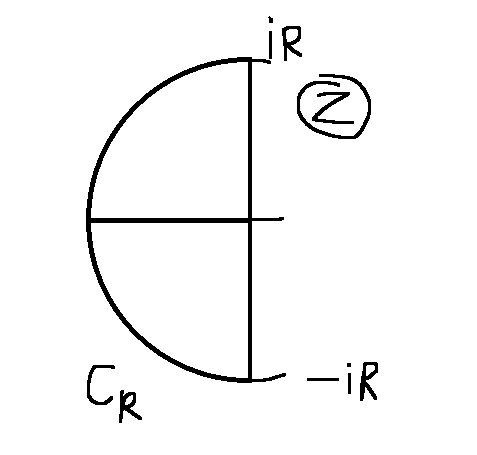
\includegraphics[width=5 cm]{graphic 2.png}

Построим замкнутый контур $C_R$ (см. рисунок). Положим $f(z) = z + \lambda,\ g(z) = -e^z$. На отрезке $[-iR, iR]$ имеем
$$\left. \begin{matrix}
|f(z)| = |\lambda + z| = |\lambda + iy| \geqslant \lambda > 1 \\ |g(z)| = |e^{iy}| = 1
\end{matrix} \right\} \Rightarrow |f| > |g|$$
По теореме Руше $N_f = N_g+f$. Так как $N_f = 1,\ (z = -\lambda$, то и исходное уравнение в области, ограниченной контуром $C_R$, имеет один корень. Ясно, что больше корней быть не может, так как $|f| > |g|$ выполняется для ... /дальше текста не видно. Решите сами, упражнение для читателя/



\section{Определение конформного отображения}

\hspace{14pt} При определении геометрического смысла модуля и аргумента производной ФКП было дано определение конформного отображения.
\par\bigskip

\textbf{Определение}

Взаимно однозначное отображение области $D$ комплексной плоскости $Z$ на области из комплексной плоскости $W$ называется конформным, если это отображение во всех точках $z\in D$ обладает свойствами сохранения углов и постоянства растяжений.
\par\bigskip

Слова "взаимно однозначное отображение" означают, что $f$ --- биекция, то есть отображение должно быть однозначным (каждому $z$ отвечает только одно $w$) и инъективным: различным $z_1$ и $z_2$ соответствуют и различные $w_1$ и $w_2$. Инъективные отображения в т ФКП, как мы уже знаем,называют однолистными, и мы эту терминология тоже сохраним.

Если внимательно проанализировать определение, то можно сделать вывод, что конформное отображение --- это отображение, сохраняющее формы малых фигур.

В этой же лекции (о геометрическом смысле производной) было показано, что если функция $w = f(z)$ является однозначной (в дальнейшем рассматривать будем только однозначные функции) однолистной голоморфной в точке $z_0$, причём $f'(z_0) \not= 0$, то отображение осуществляемое функцией $f$ будет конформным в окрестности точки $z_0$.

Угол между двумя любыми гладкими кривыми, проходящими через точку $z_0$ при отображении $w = f(z)$ не меняется ни по величине, ни по направлению отсчёта, а линейные элементы в точке $z_0$ преобразуются подобным образом.

Отметим,  простейшие свойства конформных отображений, вытекающих непосредственно из определения и свойств однолистных и обратных функций.
\par\bigskip

\textbf{Свойства:}
\begin{enumerate}
    \item Отображение, обратное к конформному, также является конформным.
    \item Композиция двух конформных отображений представляет собой конформное отображение.
    \item Функция $f$, осуществляющая конформное отображение области $D$ на область $W$ может иметь в качестве особой точки не более одного полюса в $D$.
\end{enumerate}


Понятие конформности отображения вводится и для бесконечно удалённой точки.
\par\bigskip

\textbf{Углом между кривыми} $\gamma_1$ и $\gamma_2$, \textbf{проходящими через точку} $z = \infty$, называется угол между образами этих кривых при отображении $\xi = \frac{1}{z}$ в точке $\xi = 0$.
\par\bigskip

Из этого определения и определения конформного отображения вытекает, что отображение $w = \frac{1}{z}$ сохраняет углы между кривыми в каждой точке расширенной комплексной плоскости.

Под конформностью в бесконечно удалённой точке ($z_0 \rightarrow \infty$ или $\infty \rightarrow w_0$ понимают отображение, которое только сохраняет углы между кривыми.
\par\bigskip
Отображение $w = \frac{1}{z}$ конформно во всех точках расширенной комплексной плоскости.
\par\bigskip

\textbf{Пример.} \quad
Пусть два луча выходят из одной и той же конечной точки $z_0$. Тогда угол между этими лучами в точке $z = \infty$ равен углу в точке $z_0$, взятому с обратным знаком.
\par\bigskip

Действительно, для простоты ограничимся случаем $z_0 = 0$.

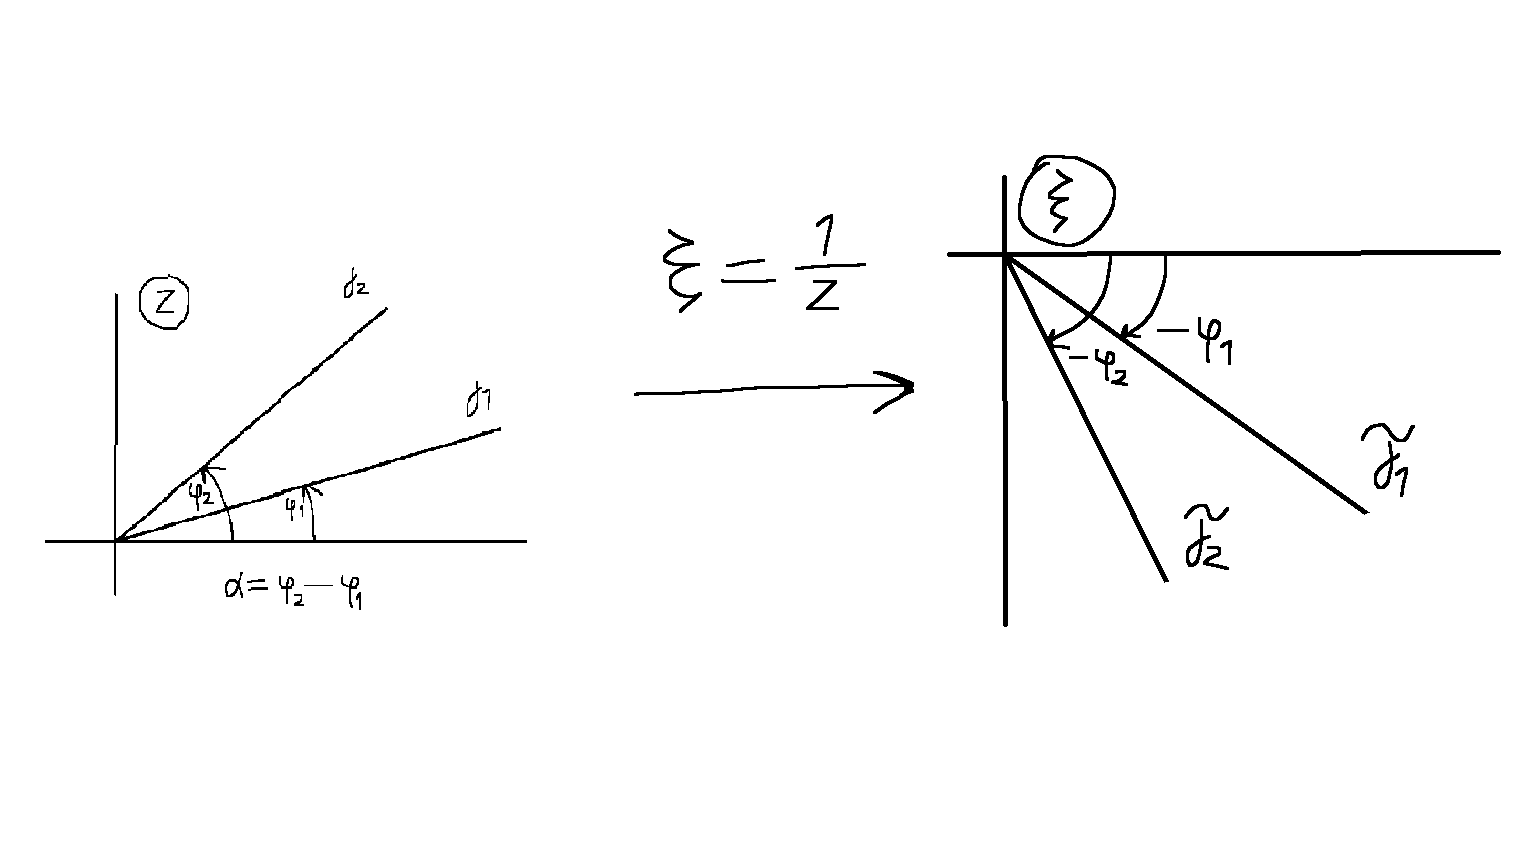
\includegraphics[width=15 cm]{graphic.png}

Угол между $\tilde \gamma_2$ и $\tilde \gamma_1$ в точке $\xi = 0$ равен $(-\phi_2)-(-\phi_1) = -(\phi_2 - \phi_1) = -\alpha$




\section{Необходимое и достаточные условия конформности}

\hangindent=11pt \hangafter=0 \noindent
\textbf{Достаточные условия конформности}
(Нам уже известны)

\textit{Если функция \(w = f(z)\)  является однозначной и однолистной голоморфной функцией в области \(D\) и \(f'(z) \neq 0,  \forall z \in D\) , то отображение \(w = f(z)\) конформно в области \(D\) }
\bigskip

\hangindent=11pt \hangafter=0 \noindent
\textbf{Необходимые условия конформности}
\textit{Пусть функция \(w=f(z)\)  осуществляет конформные отображения области \(D\) комплексной плоскости \textcircled{z} на область  из комплексной плоскости \textcircled{w} и ограничена в \(D\). Тогда функция \(f(z)\) является однолистной и голоморфной в \(D\), причем \(f'(z) \neq 0,  \forall z \in D\)  }

\begin{Proof}
Поскольку отображение конформно, то функция \(w = f(z)\)  однозначна и однолистна.
\begin{center}
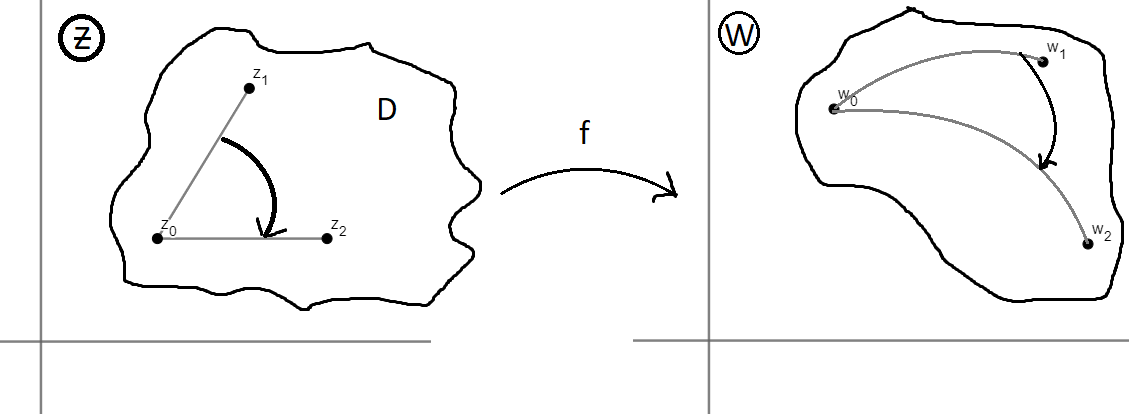
\includegraphics[width=0.5\linewidth]{conform/theorem_figure.png}
\end{center}
Возьмём две точки \(z_1\) и \(z_2\) в области \(D\),  лежащей в некоторой окрестности фиксированной точки \(z_0\):

\[
z_0: \; z_0\xrightarrow{f(x)} w_0, \:z_1\xrightarrow{f(x)} w_1, \: z_2\xrightarrow{f(x)} w_2
\] 

Так как  отображение конформно, что углы между кривыми сохраняются.

Следовательно, \(arg\Delta z_2 - arg\Delta z_1 = arg\Delta w_2 - arg\Delta w_1 \) с точностью до бесконечно малых более высокого порядка чем \(\Delta z\)
\[\text{(Здесь } \Delta z_1 = z_1 - z_0, \;\Delta z_2 = z_2 - z_0, \; \Delta w_1 = w_1 - z_0,\; \Delta w_2 = w_2 - w_0 \text{)}\]
отсюда следует, что:
\[
arg\Delta w_2 - arg\Delta z_2 = arg\Delta w_1 - arg\Delta z_1 
\]
\begin{center}
или  
\end{center}
\[
 arg \frac{\Delta w_2}{\Delta z_2} = arg \frac{\Delta w_1}{\Delta z_1} =:: \alpha
\]

Причём равенство справедливое с точностью до бесконечно малых более высокого порядка чем \(\Delta z\). 

В силу же постоянства растяжений:
\[
\frac{|\Delta w_2|}{|\Delta z_2|} = \frac{|\Delta w_1|}{|\Delta z_1|} =:: k \neq 0
\]
c точностью до бесконечно малых более высокого порядка чем \(\Delta z\).
Поэтому, объединяя, получим:
\[
\frac{\Delta w_2}{\Delta z_2} = \frac{\Delta w_1}{\Delta z_1} =:: k\cdot e^{i\alpha} \neq 0
\]В силу произвола выборе точек \(z_1, z_2\) отсюда следует, что \(\frac{\Delta w}{\Delta z} = ke^{i\alpha} + o(\Delta z)\) это означает что что проведенное рассуждение годится для \(\forall z_0 \in D\), значит \(f \text{ - голоморфна в } D \text{ и } f'(z) \neq 0, \forall z \in D\)
\end{Proof}

\par\bigskip
\textbf{Замечание 1.} \quad Следует отметить, что условие голоморфности \(f\) с \(f(z)\neq 0\)  являются необходимыми, но недостаточными условиями голоморфности.

Если \(f\) голоморфна и \(f'(z) \neq 0\), но \(f\) неоднолистна, то отображение \(f\) не является конформным.

Приведём пример иллюстрирующий это утверждение:

\includegraphics[width=6 cm]{conform/example.png}

Функция \(w =z ^ 4\)  заданная в полукольце \(1 \leq z \leq 2, \; 0 \leq arg\,z \leq \pi\). Функция голоморфна: \(w' = 4z^3\neq 0\). Функция отображает полукольцо на кольцо \(B(0,\,1,\,16), \: 0 \leq arg\,w\leq 4\pi\). Нарушается взаимно-однозначное и, следовательно, отображение не может быть конфорным.

\par\bigskip
\textbf{Замечание 2.} \quad Поскольку отображение \(w = \frac{1}{z}\) комфортно в точке \(z = 0\), а композиция конформных отображений конформно, то если функция \(w = f(z)\) даёт конформное отображение, то \(w = f(\frac{1}{z})\) тоже комфортно. Это говорит о том, что функция дающий конформное отображение области \(D\) на область \(G\)  должна быть голоморфной в области \(D\) за исключением может быть особой точки, в которой может быть полюс первого порядка.


\section{Принцип взаимно-однозначного соответствия}

\hangindent=11pt \hangafter=0 \noindent \textbf{Теорема}
\textit{Пусть функция \(w = f(z)\) является однозначной и голоморфной в области \(D\)  и осуществляет взаимно-однозначное отображение области \(D\) на область \(G\). Тогда это отображение будет конформным в области \(D\)}
\begin{Proof}
Следует показать, что \(f\) - однолистная функция и \(f'(z)\neq 0, \forall z \in D\). Однолистность следует из того, что \(f\) - взаимно-однозначная, то есть биекция.

Докажем, что \(f'(z)\neq 0 \) в \(D\).

Предположим от противного, что \(\exists z_0 \in D\), что \(f'(z_0) = 0\). Так как \(f\) голоморфна в \(D\), то её разложение в ряд по степеням \(z - z_0\) имеет вид:
\[
	f(z) = c_0 + c_k(z - z_0) ^k + c_{k+1}(z-z_0)^{k+1}+..., \; \text{где } k>1 \text{ и }
 c_k \neq 0\]
 
 Точка \(z_0\)не может быть предельной точкой нулей функции \(f'(z)\), так как нули голоморфной функции изолированны, а \(f'(z) \neq const\), в силу условий теоремы. Поскольку \(z_0\) изолированный ноль функции \(f'(z)\), то:
\[
	\exists \delta_1 > 0, \: f'(z) \neq 0, \: \forall z \in \overline{B}(z_0, 0, \delta_1)
\]

Рассмотрим функцию \(\phi(z) ::= c_k + c_{k+1}(z-z_0)+...\)  Так как \(c_k \neq 0\), то в силу непрерывности функции \(\phi(z)\):
\[
\exists \delta_2, \: \phi(z) \neq 0, \: \forall z \in \overline{B}(z_0,\delta_2)
\]

Обозначим \(\delta ::= min\:\{\delta_1, \delta_1\}\) 

Тогда в кольце \(\overline{B}(z_0, 0, \delta)\) одновременно выполняются оба условия, то есть \(f'(z)\neq 0 \text{ и } \phi(z) \neq 0\).

Обозначим \(m ::= \min \limits_{z\in S(z_0, \delta)} |(z-z_0)^k\phi(z)|>0\)

Возьмем произвольное комплексное число \(\alpha\), удовлетворяющее условию \(|\alpha| < m\).
Тогда функции \((z-z_0)^k\phi(z) \text{ и } ((z-z_0)^k\phi(z)  - \alpha = f(z) - c_0 - \alpha\) голоморфны в замкнутом круге \(\overline{B}(z_0,\delta) \) и на его границе \(S(z_0,\delta_2)\) удовлетворяют условию:

\[
	|(z-z_0)^k\phi(z)|\geq m > |\alpha|
\]

На основании теоремы Руше функции \((z-z_0)^k\phi(z) \text{ и } f(z) - c_0 - \alpha\) имееют в круге \(B(z_0,\delta) \) одинаковое число нолей, а именно, к нолей, а именно, к нолей где \(k > 1\). То есть: уравнение \(f(z)-c_0-\alpha\) имеет \(k\) корней в круге \(B(z_0,\delta) \), причём все эти корни простые, так как \(z=z_0\) не является корнем этого уравнения, а \(f'(z)\neq 0\) во всех точках \(B(z_0,\delta)  \setminus \{z_0\}\). Это означает, что в различных точках круга \(B(z_0,\delta) \subset D\) функция \(f\) принимает одно и то же значение а именно \(c_0 + \alpha\) , что противоречит условию взаимной однозначности отображения \(f: \; D \rightarrow G\).
\end{Proof}




\section{Принцип соответствия границ}
При решении конкретных задач на конформные отображения чаще всего достаточно выяснить, во что переходят при отображении границы и не обязательно исследовать все внутренние точки. Это возможно в силу так называемого \textbf{принципа соответствия границ:}
\quad\bigskip

\textit{Пусть в конечной области D, ограниченной простым замкнутым контуром $\partial D$, задана голоморфная функция $w=f(z)$, непрерывная в $\overline{D}$, которая осуществляет взаимно-однозначное отображение контура $\partial D$ на некоторый  контур L комплексной плоскости \textcircled{w}. Если при этом сохраняется направление обхода контуров, то f конформно отображает область D на область G, ограниченную контуром $L=\partial G$.}
\par
\begin{center}
    \includegraphics[width=8 cm]{borders.png}
\end{center}

\begin{Proof}
    Воспользуемся принципом взаимно-однозначного соответствия. Тогда для доказательства теоремы достаточно показать, что f устанавливает взаимно-однозначное соответствие между областями D и G, т.е.:

\begin{enumerate}
    \item Каждому $z\in D \  f$ ставит в соответсвие некоторую точку $w \in G$
    \item Для каждого $w_1 \in G$ найдется единственная точка $z_1 \in D$ такая, что $f(z_1)=w_1$.
\end{enumerate}
\par\bigskip
Возьмем 2 произвольные точки, $w_1 \in G$ и $w_2 \in \mathbb{C}\setminus \overline{G}$ и построим в области D две функции:
$$F_1(z)=f(z)-w_1, z\in D$$
$$F_2(z)=f(z)-w_2, z\in D$$

Посчитаем число нулей для этих функций в области D. Для этого воспользуемся принципом аргумента. Отметим сначала,что $F_1, F_2$ не обращаются в ноль на контуре $\partial D$, т.к. при $z \in \partial D$ точка $w=f(z) \in L$, а мы взяли $w_1 \in G$ и $w_2 \in \mathbb{C}\setminus \overline{G}$
$$N_{F_1}=N_{f-w_1}=\frac1{2\pi} \Delta_{\partial D} \ arg(f(z)-w_1)= \frac1{2\pi} \Delta_L \ arg(w-w_1)=1$$

$$N_{F_2}=N_{f-w_2}=\frac1{2\pi} \Delta_{\partial D} \ arg(f(z)-w_2)= \frac1{2\pi} \Delta_L \ arg(w-w_1)=0$$

Из первого соотношения получаем, что уравнение $f(z)=w_1$ имеет лишь один корень, т.е. $\exists ! z \in D$, такая, что $f(z)=w_1$.

Второе соотношение показывает, что уравнение $f(z)=w_2$ не имеет корней в области D, следовательно, у точки $w_2$ нет прообраза в D, т.е. $\{f(z)|z\in D\}\subset G$

Все это вместе и означает биекцию, и по предыдущему пункту f конформно.
\end{Proof}

\quad\bigskip

\textbf{Замечание 1.} \quad Если f регулярна в D за исключением точки $z_0$, в которой она имеет простой полюс, и $\partial D \to \partial G$ c изменением направления обхода, то D отображается конформно на внешность $\partial G$.
\par\bigskip
\textbf{Замечание 2.} \quad
Имеет место и такое утверждение:\par
Если f отображает конформно D в G, а D, G -- конечные области(граница G не содержит бесконечно удаленную точку), то f непрерывна на $\partial D$ и осуществляет непрерывное и взаимно-однозначное соответствие между точками контуров, причем направление обхода сохраняется.
\par\bigskip
\textbf{Замечание 3.} \quad Теорема имеет место и в случае, когда D и G -- неограниченные области.





\section{Оригинал и изображение}
Преобразование Лапласа возникло из так называемого символического исчисления, которое было ещё популярным в прошлом веке. В его основе лежали формальные операции над символом $p = \dfrac{d}{dt}$. Например. положительная степень $n$ символа $p$ означала $n - $ую производную функции $p^n\cdot x = \dfrac{d^nx(t)}{dt^n}$, а отрицательная степень - интеграл:

\begin{center}
    $\dfrac{1}{p}x = \int\limits_0^tx(\tau)d\tau$
\end{center}

Применение этого символа к функции $x(t) \equiv 1$ приводит к равенствам:

\begin{center}
    $\dfrac{1}{p}\cdot1 = \int\limits_0^tdt = t; \dfrac{1}{p^2} = \int\limits_0^t\tau d\tau = \dfrac{\tau^2}{2}, ..., \dfrac{1}{p^n}\cdot1 = \dfrac{t^n}{n!}$
\end{center}

Популяризовал его инженер-электрик Оливер Хевисайд. Как оно применялось практически? К примеру, уравнение $\dfrac{dx}{dt} - x = 1$ с условиями $x(0) = 0$ заменялось символическим уравнением $px - x = 1$. Отсюда $x = \dfrac{1}{p - 1} = \dfrac{1}{p} \cdot \dfrac{1}{1 - \dfrac{1}{p}} = \dfrac{1}{p}(1 + \dfrac{1}{p} + \dfrac{1}{p^2} + ... + \dfrac{1}{p^n} + ...) = \int\limits_0^t(1 + \tau + \dfrac{\tau^2}{2!} + ... + \dfrac{\tau^n}{n!} + ...)d\tau = \int\limits_0^t e^{\tau}d\tau = e^t - 1$.\par Можете проверить, что ответ получится правильным.
\par\bigskip
Метод работы над символом $p$ не обосновывался, но иногда приводил к неверным результатам. Лишь в 20-ые годы 20-го века математикам надоело такое положение вещей и метод получил обоснование в работах Бромвича и Карсона и стал называтся операционным методом.

Суть его в том, что дифференцирование и интегрирование заменяются алгебраическими операциями, диффиренциальные уравнения --- алгебраическими и т.д.

Основан операционный метод на преобразовании Лапласа, которое ставит в соответствие функции $f(t)$ действительного переменного $t$ функцию $\digamma(p)$ комплексного переменного $p$ с соотношения:

\begin{center}
    $\digamma(p) = \int\limits_0^{+\infty}f(t)e^{-pt}dt (1)$
\end{center}

$p$ --- комплексный параметр, $p = x + iy$.

Интеграл в правой части $(1)$ --- интеграл Лапласа функции $f$, а функция $\digamma(p)$ --- преобразование Лапласа или первообразная по Лапласу. Иногда преобразованием Лапласа называют процесс нахождения функции $\digamma$.

Мы будем пользоваться следующей терминологией: $f(t)$ --- оригинал, $\digamma(p)$ --- изображение. Для обозначения того, что $\digamma$ изображение оригинала $f$ употребляются записи $\digamma(p)\rightarrow f(t), \digamma(p)\rightarrow Lf(t), f(t) = L^{-1}\digamma(p), \digamma(p) \dot{\rightarrow}f(t)$. Мы будем использовать:

\begin{center}
    $f(t) \risingdotseq \digamma(p), \digamma(p) \risingdotseq f(t)$
\end{center}

\textbf{Примеры: }
\begin{enumerate}
    \item $f(t) = 1,\; \digamma(p) = \int\limits_0^{+\infty}1\cdot e^{-pt}dt = -\dfrac{1}{p}e^{-pr}\Bigr|_0^{+\infty} = \dfrac{1}{p}$. \quad Т.е. $1 \risingdotseq \dfrac{1}{p}$.
    
    Заметим, однако, что это верно, если $Re(p) = x > 0$. При $x \leq 0$ интеграл не существует. Однако, функция $\dfrac{1}{p}$ регулярна во всей области комплексного переменного $p$, за исключением $p = 0$ и её значения для $Re(p) < 0$ можем рассматривать как значения изображения $\digamma(p)$ при $Re(p) < 0$. Тогда равенство $1 \risingdotseq \dfrac{1}{p}$ будет иметь место $\forall p$ (аналогично тому, как мы рассматривали $\Gamma$ функцию для отрицательных значений аргумента).
    
    \item $f(t) = e^{t^2}$.
    
    Функция не имеет изображения, т.к. при достаточно больших $t$ $e^{t^2}\cdot e^{-pt} > 1$. При действительных $p$ и интеграл Лапласа расходится.
\end{enumerate}

Примеры показывают, что изображение может существовать, а может и не существовать. Поэтому важно уметь выделять классы функций, являющихся оригиналами.
\par\bigskip
В операционном исчислении принято рассматривать функции, которые удовлетворяют следующим условиям:

\begin{enumerate}
    \item $f(t)$ задана на $R$, причём $f(t) = 0, \forall t < 0$
    \item $f(t)$ --- кусочно-непрерывна на $R$, т.е. на любом конечном промежутке имеет не более конечного числа точек разрыва, причём только первого рода
    \item При $t \rightarrow \infty$ функция $f$ имеет ограниченную степень роста, т.е. существуют такие постоянные $\alpha$ и $M = M(\alpha)$, что $|f(t)| \leq Me^{\alpha t}, \forall t > 0$.
\end{enumerate}

Точная нижняя грань всех $\alpha$, для которых выполняется последнее неравнество, т.е. число $\alpha_0 = inf{\alpha}$ называется \textbf{показателем степени роста $f$}.
\par\bigskip
Отметим, что при $\alpha = \alpha_0$ неравенство может и не выполняться. Например, $f(t) = t$. $t \leq e^{\alpha t}, \forall \alpha > 0, \alpha_0 = 0, t \leq 1 ??$ --- неверно. Однако, оно будет справедливым $\forall \alpha > \alpha_0$.

\par\bigskip
В дальнейшем эти условия, которые мы накладываем на $f$ будет называть \textbf{О -- условиями} и называние 'оригинал' употреблять только для функций, удовлетворяющих О --- условиям. Хотя, как будет отмечено в дальнейшем, функция может быть оригиналом и не удовлетворять О -- условиям. Дело в том, что для функций, удовлетворящим О --- условиям, всегда существует изображение и оно обладает широким спектром свойств.

\par\bigskip
\textbf{Пример.} \quad $\dfrac{1}{\sqrt{t}}$ не удовлетворяет О -- условиям, однако, интеграл (1) сходится, т.е. $\dfrac{1}{\sqrt{t}}$ является оригиналом.
\par\bigskip
Таким образом, как мы покажем ниже, О -- условия являются лишь достаточными условиями для существования изображения, но не необходимыми.

\par\bigskip

Эти условия хороши тем, что их выполнение гарантирует справедливость ряда теорем, составляющих основное содержание операционного исчисления.

В приложениях операционное исчисление используется главным образом для решения дифференциальных уравнений, удовлетворяющих некоторым начальным условиям. Т.к. за начальный момент всегда можно принять момент $t = 0$, а что происходит до начального момента, физиков чаще всего не интересует, то условие $f \equiv 0, t < 0$ не является обременительным, а условия 2, 3 для функций, используемых в приложениях, чаще всего выполняются.

\par\bigskip
Одной из простейших функций, удовлетворящющих О -- условиям, является функция Хевисайда.

\begin{center}
 $1(t) = $ 
 \begin{cases}
   1, & $t \geq 0$\\
   0 & $t < 0$$}
 \end{cases}
\end{center}

Показатель роста $\alpha_0 = 0$. Изображение её, по сути, мы нашли в примере 1:

\begin{center}
    $1(t) \risingdotseq \dfrac{1}{p}$
\end{center}
\par\bigskip



    \section{Достаточные условия существования изображения}

\textbf{Теорема.}\ \textit{Всякий оригинал $f(t)$, удовлетворяющий О --- условиям, имеет изображение. Это изображение $\digamma(p)$ есть фукнция регулярная в полуплоскости $Re(p) > \alpha_0$, где $\alpha_0$ - показатель степени роста $f$}.
\begin{Proof}
    Пусть $f$ --- оригинал, удовлетворяющий О --- условиям и $\alpha_0$ --- его показатель степени роста. Рассмотрим $p$ такое, что $Re(p) > \alpha_0, p = x + iy$. Выберем $\varepsilon > 0$ так, чтобы $x = Re(p) > \alpha_0 + \varepsilon$. Тогда справедлива оценка:

$|\digamma(p)| = |\int\limits_0^{+\infty} e^{-pt}f(t)dt| \leq \int\limits_0^{+\infty} e^{-xt}|f(t)|dt \leq \int\limits_0^{+\infty} e^{-xt}Me^{(\alpha_0 + \varepsilon)t} = M\cdot\int\limits_0^{+\infty} e^{(-x + \alpha_0 + \varepsilon)t} = \dfrac{Me^{(-x + \alpha_0 + \varepsilon)t}}{\alpha_0 - x + \varepsilon}\Bigr|_0^{+\infty} = \dfrac{M}{x - \alpha_0 - \varepsilon} (2)$
\par\bigskip
Из неравенства (2) вытекает, что функция $\digamma(p)$ мажорирует абсолютно сходящимся интегралом, что означает сходимость, т.е. существование изображения $\digamma(p)$.

Если же $x \geq x_0 > \alpha_0$, то согласно (2) приходим к оценке:

\begin{center}
    $|\digamma(p)| < \dfrac{M}{x_0 - \alpha_0 - \varepsilon} = \Bigr[ \varepsilon := \dfrac{x_0 - \alpha_0}{2} \Bigr] = \dfrac{M_1}{x_0 - \alpha_0}$
\end{center}

что означает равномерную сходимость интеграла Лапласа $\forall p$, удовлетворяющих условию $Re(p) \geq x_0 > \alpha_0$.

\par\bigskipДругими словами, интеграл Лапласа сходится локально равномерно в полуплоскости $Re(p) > \alpha_0$

\begin{center}
    \includegraphics[width=13 cm]{original/shodimost.png}
\end{center}
\parДалее разобъём $[0; +\infty)$ точками $0 = t_0 < t_1 < ... < t_n < ..., n \rightarrow \infty$ на отрезки $[t_{k-1}, t_k]$, на которых функция $f$ непрерывна, и представим $\digamma(p)$ в виде ряда:

\begin{center}
    $\digamma(p) = \int\limits_0^{+\infty}f(t)e^{-pt}dt = \sum\limits_{k=1}^{+\infty}\int\limits_{t_{k-1}}^{t_k}f(t)e^{-pt}dt = \sum\limits_{k=1}^{+\infty}\digamma_k(p)$
\end{center}

Этот ряд сходится локально равномерно в полуплоскости $Re(p) > \alpha_0$, т.к. там сходится локально равномерно соответствующий интеграл. Члены этого ряда являются функциями регулярными в этой полуплоскости. Действительно:

$\digamma'_k(p) = \lim\limits_{\Delta p \rightarrow 0}\dfrac{\digamma_k(p + \Delta p) - \digamma(p)}{\Delta p} = \lim\limits_{\Delta p \rightarrow 0} \dfrac{1}{\Delta p}(\int\limits_{t_{k-1}}^{t_k}f(t)e^{-(p + \Delta p)t})dt - \int\limits_{t_{k-1}}^{t_k}f(t)e^{-pt} = $ 

$ = \lim\limits_{\Delta p \rightarrow 0}\int\limits_{t_{k-1}}^{t_k}f(t)e^{-pt}\dfrac{e^{-\Delta pt} - 1}{\Delta p}dt = \lim\limits_{\Delta p \rightarrow 0}\int\limits_{t_{k-1}}^{t_k}f(t)e^{-pt}\dfrac{-\Delta pt}{\Delta p}dt = -\int\limits_{t_{k-1}}^{t_k}tf(t)e^{-pt}dt$ --- есть непрерывная функция $p$. Это означает, что производная $\digamma'_k$ существует и непрерывна $\Rightarrow \digamma_k$ регулярная функция $p$.

По теореме Вейерштрасса и сумма ряда будет функцией регулярной в $Re(p) > \alpha_0$
\end{Proof}
\par\bigskip

\textbf{Замечания}

\begin{enumerate}
    \item Можно показать, что если интеграл Лапласа сходится при $p = p_0$, то $\digamma(p)$ --- регулярна в полуплоскости $Re(p) > Re(p_0)$
    \item Фукнцию $\digamma(p)$ регулярную при $Re(p) > \alpha_0$ чаще всего можно аналитически продолжить на более широкую область. Обычно $\digamma(p)$ оказывается регулярной во всей комплексной плоскости за исключением некоторого числа изолированных особых точек, причём все они лежат в полуплоскости $Re(p) \leq \alpha_0$
    \item Из формулы (2) следует, что $|\digamma(p)| \rightarrow 0$ при $Re(p) \rightarrow \infty$
    \item Из теоремы следует, что не всякая функция $\digamma(p)$ может служить изображением какой-либо функции, являющейся оригиналом. Например, $tg(p)$ имеет бесконечное множество полюсов $p_k = \dfrac{2k - 1}{2}\pi$ и нельзя указать полуплоскости $Re(p) > \alpha$, где $tg(p)$ --- изображение. Или $p, p^2, sqrt(p), sin(p)$ не изображения, т.к. не стремятся к нулю при $p \rightarrow \infty$
    \item Преобразование Хевисайда: $\digamma^*(p) = p\digamma(p)$
\end{enumerate}


\section{Изображения некоторых функций}
\subsection*{$1) \quad 1(t) \risingdotseq \frac{1}{p}$}
В дальнейшем под функцией $f(t)$ будем понимать функцию $1(t) \cdot f(t)$, т.е. равную нулю для $t < 0$ и равную $f(t)$ для $t > 0$. Для удобства $1(t)$ писать не станем.

\subsection*{$2)$\quad\textsl{Экспонента} $f(t) = e^{at}$}
Показатеь степени роста, очевидно, $Re$ $p > Re$ $a$.
\par\bigskip
\begin{center}
    $e^{at} \risingdotseq \frac{1}{p - a}$, $Re$ $p > Re$ $a$.
\end{center}
\par\bigskip
\subsection*{$3)$\quad\textsl{Степенная функция} $f(t) = t^\nu$, $\nu \in \mathbb{R}$}

Показатель степени роста $\alpha_0 = 0$.
\par\bigskip
$\mathcal{F}(p) = \int\limits_{0}^{+\infty} t^{\nu}  e^{-pt}\, dt$.
\par\bigskip
Сначала предположим, что $p$ - действительное. Тогда:
\par\bigskip
$\mathcal{F}(p) = \int\limits_{0}^{+\infty} t^\nu e^{-pt}\,dt = \biggl[ pt = \tau, dt = \frac{d\tau}{p} \biggr] = \frac{1}{p^{\nu + 1}} \int\limits_{0}^{+\infty} \tau^\nu e^{-\tau}\,d\tau = \frac{\Gamma(\nu + 1)}{p^{\nu + 1}}$, $p > 0$.
\par\bigskip
Отметим, что $\mathcal{F}(p)$ существует для для $\nu > -1$, хотя $f(t) = t^\nu$, $\nu > -1$ и не удоволетворяет $O$ -  условиям.
\par\bigskip
Анализируя $\mathcal{F}(p)$, видим, что $\mathcal{F}(p)$ существует для $\forall p > 0$, т.е.  $\frac{\Gamma(\nu + 1)}{p^{\nu + 1}}$ голоморфна для $\forall p > 0$. Такую функцию называют аналитическим продолжением $\mathcal{F}(p)$ с действительной оси и впоследствии мы покажем, что в такой ситуации формула справедлива для $\forall p$ таких, что $Re$ $p > 0$. Итак:
\begin{center}
    $t^\nu \risingdotseq \frac{\Gamma(\nu + 1)}{p^{\nu + 1}}$, $Re$ $p > 0$, $\nu > -1$
\end{center}
\par\bigskip
если $\nu = n  \in \mathbb{N}$, то
\begin{center}
    $t^n \risingdotseq \frac{n!}{p^{n + 1}}$, $Re$ $p > 0$
\end{center}


\section{Свойства изображений}
\subsection*{1) Линейность изображения}
\par
\textsl{Если}
\par\bigskip
\begin{center}
$f_1 \risingdotseq \mathcal{F}_1, $ $Re$ $p > \alpha_1$
\par
$f_2 \risingdotseq \mathcal{F}_2, $ $Re$ $p > \alpha_2$,
\end{center}
\par
\textsl{то:}
\begin{center}
\par 
$c_1 f_1 + c_2 f_2 \risingdotseq c_1 \mathcal{F}_1 + c_2 \mathcal{F}_2$\,, $Re$ $p > \max\{\alpha_1, \alpha_2\}$
\end{center}
\par\bigskip
$\blacklozenge$ \quad Следует из линейности интеграла Лапласа \quad $\blacksquare$
\par\bigskip
\textbf{Примеры:}
\begin{center}
$1)$ $\ch{t} = \frac{e^t + e^{-t}}{2} \risingdotseq \frac{1}{2} (\frac{1}{p - 1} + \frac{1}{p + 1}) = \frac{p}{p^2 - 1}$
\par\bigskip
$2)$ $\sh{t} = \frac{e^t - e^{-t}}{2} \risingdotseq \frac{1}{2} (\frac{1}{p - 1} - \frac{1}{p + 1}) = \frac{1}{p^2 - 1}$
\par\bigskip
$3)$ $\cos{t} = \frac{e^{it} + e^{-it}}{2} \risingdotseq \frac{1}{2} (\frac{1}{p - i} + \frac{1}{p + i}) = \frac{p}{p^2 + 1}$
\par\bigskip
$4)$ $\sin{t} = \frac{e^{it} - e^{-it}}{2i} \risingdotseq \frac{1}{2i} (\frac{1}{p - i} + \frac{1}{p + i}) = \frac{1}{p^2 + 1}$
\end{center}
\par\bigskip
\subsection*{2)Теорема подобия }
\par
\textsl{Если}
\begin{center}
$f(t) \risingdotseq \mathcal{F}(p), $ $Re$ $p > \alpha_0$ и $\lambda > 0$
\end{center}
\par
\textsl{то:}
\begin{center}
\par 
$f(\lambda t) \risingdotseq \frac{1}{\lambda} \mathcal{F}(\frac{p}{\lambda}), $ $Re$ $p > \alpha_0 \lambda$
\end{center}
\par\bigskip
$\blacklozenge$ \quad $f(\lambda t) \risingdotseq \int\limits_{0}^{+ \infty} f(\lambda t) e^{-pt}\, dt = \biggl[\lambda t = \tau, dt = \frac{d\tau}{\lambda} \biggr] = \frac{1}{\lambda} \int\limits_{0}^{+\infty} f(\tau) e^{-\frac{p\tau}{\lambda}}\, d\tau = \frac{1}{\lambda} \mathbb{F}(\frac{p}{\lambda})$ \quad $\blacksquare$
\par\bigskip
\textbf{Примеры:}
\begin{enumerate}
    \item $\cos{\omega t} \risingdotseq \frac{1}{\omega} \cdot \frac{\frac{p}{\omega}}{\frac{p^2}{\omega^2} + 1} = \frac{p}{p^2 + \omega^2}$
    \item $\sin{\omega t} \risingdotseq \frac{\omega}{p^2 + \omega^2}$
    \item $\sh{\omega t} \risingdotseq \frac{\omega}{p^2 - \omega^2}$
    \item $\ch{\omega t} \risingdotseq \frac{p}{p^2 + \omega^2}$
\end{enumerate}

\par\bigskip
\subsection*{3) Теорема запаздывания }
\par
\textsl{Если}
\begin{center}
$f(t) \risingdotseq \mathcal{F}(p), $ $Re$ $p > \alpha_0$
\end{center}
\par
\textsl{то:}
\begin{center}
\par 
$f(t - a) \risingdotseq e^{-pa} \mathcal{F}(p), $  где $f(t-a) \equiv 0, $ $t < a$ 
\end{center}
\par\bigskip
$\blacklozenge \quad f(t - a) \risingdotseq \int\limits_{a}^{+ \infty} f(t - a) e^{-pt}\, dt = \biggl[ t - a = \tau \biggr] = \int\limits_{0}^{+ \infty} f(\tau) e^{-ap} e^{-p\tau}\, d\tau = e^{-ap}\mathcal{F}(p) \quad \blacksquare$
\par\bigskip

\subsection*{4) Теорема смещения}
\par
\textsl{Если}
\begin{center}
$f(t) \risingdotseq \mathcal{F}(p), $ $Re$ $p > \alpha_0$
\end{center}
\par
\textsl{то:}
\begin{center}
\par 
$e^{\beta t}f(t) \risingdotseq \mathcal{F}(p - \beta),\, \beta \in \mathbb{C}, \, Re \, p > \alpha_0 + Re \, \beta$ 
\end{center}
\par\bigskip
$\blacklozenge \quad e^{\beta t}f(t) \risingdotseq \int\limits_{0}^{+ \infty} f(t) e^{\beta t} e^{-pt}\, dt = \mathcal{F}(p - \beta) \quad \blacksquare$


\subsection*{5) Изображение производной}
\textit{Если} $f(t) \risingdotseq F(p), Rep > \alpha_0$ и $f'(t)$ \textit{является оригиналом, то} 
$$f'(t) \risingdotseq pF(p) - f(t_0)$$
\begin{Proof}
    $f'(t) \risingdotseq \int\limits_{0}^{+\infty} f'(t)e^{-pt}\, dt = \begin{bmatrix} u = e^{-pt} \quad dv = f'(t)dt\\ du = -pe^{-pt}dt \quad v = f(t) \end{bmatrix} = f(t)e^{-pt}\  \bigg|_{0}^{+\infty}\ +
    p \int\limits_{0}^{+\infty} f(t)e^{-pt}\,dt = pF(p) - f(t_0)$
\end{Proof}
\par\bigskip 
\textbf{Следствие 1.} \quad Если $f^{(n)}(t)$ оригинал, то 
$$f^{(n)}(t) \risingdotseq p^n F(p) - p^{n-1} f(t_0) - p^{n-2} f'(t_0) - \dots - pf^{(n-2)}(t_0) - f^{(t_0)}$$
\parФормула доказывается по индукции.
\par\bigskip
В частности 
$$f''(t) \risingdotseq p^2 F(p) - p f(t_0) - f'(t_0)$$
\par\bigskip
\textbf{Следствие 2.} \quad $\lim\limits_{|p| \rightarrow \infty} p F(p) = f(t_0)$



\subsection*{6) Интегрирование оригинала}

Если $f(t)=F (p),\; Rep >\alpha_0$, \quad то 
$\int\limits_{0}^{t}f(\tau)d\tau=\dfrac{F(p)}{p}, Rep>\alpha_0$.
\begin{Proof}
    $\phi(t)::= \int\limits_{0}^{t}f(\tau)d\tau  \alpha \geq 0$

$\phi(t)$- оригинал с тем же показателем роста , что и $f(t)$. Первые два условия очевидны. \parТретье:$$|\phi(t)|\leq\int\limits_{0}^{t}|f(\tau)|d\tau\leqM\int\limits_{0}^{t}e^{\alpha\tau}d\tau=\dfrac{M}{\alpha}e^{\alpha\tau}\bigg|\limits_0^t\leq M, e^{\alpha\tau}$$

Обозначим $\Phi(p)=\phi(t),\; \phi(0)=0$.
Воспользуемся изображением производной $$\phi'(t)=p \: \Phi(p)-\phi(+0)$$ \par т.к. $\phi(t)= f(t),$ получим $$f(t)=F(p)=p\Phi(p)\rightarrow \Phi(p)=\dfrac{F(p)}{p}$$
\end{Proof}


\textbf{Пример:} \quad $1=\dfrac{1}{p}\quad\Rightarrow\quad t=\dfrac{\dfrac{1}{p}}{p}=\dfrac{1}{p^2}$

\subsection*{7) Дифференцирование изображения }
\parЕсли $f(t)= F(p),\; Rep>\alpha_0,$ то 

\begin{center}
    $F'(p)=-tf(t),\; Rep>\alpha_0$\\
    $F^{(n)}(p)=(-1)^nt^nf(t),\; Rep>\alpha_0$
\end{center}

Поскольку Т -- регулярна, то возможно дифференцирование по правилу Лейбница.

$$F'(p)=\int\limits_{0}^{+\infty}(-t\;f(t))e^{-pt}dt=-tf(t)$$ \par Дальше по индукции.
\par\bigskip
\textbf{Пример.} \quad $sint=\dfrac{1}{p^2+1}\quad \Rightarrow \quad - sint= -\dfrac{2p}{(p^2+1)^2}$

\subsection*{8) Интегрирование изображения}
Если $\dfrac{f(t)}{t}$-оригинал и $f(t)= F(p), Rep > \alpha_0,$ то $\dfrac{f(t)}{t}=\int\limits_{p}^{\infty}F(\iota)d\iota,$ причем путь интегрирования лежит в полуплоскости $ Rep\geq x_0> \alpha_0.$ 

\begin{Proof}
    Рассмотрим $$\dfrac{f(t)}{t}= J(p)=\int\limits_{f(t)}^{\tau}e^{-pt}dt. J(p)$$ \par она регулярна в $Rep>\alpha_0$, причем $J(\infty)=0.$ \par\bigskip По теореме о дифференцировании изображения $$J'(p)=(-t)\dfrac{f(t)}{t}=-f(t).$$ \parНо $f(t)=F(p).$ Поэтому $J'(p)=-F(p)$ \parт.е. $I(p)$ -есть из первообразныхдля функции $-F(p)$, причем та, которая на $\infty$ обращается в нуль. Это означает, что $$\int\limits_{p}^{\infty}(-F(s))ds=J(\infty)-J(p)=-J(p)$$ Отсюда следует: $$J(p)=\int\limits_{p}^{+\infty}F(s)ds,$$ т.е. $$\dfrac{f(t)}{t}=\int\limits_{p}{+\infty}F(s)ds.$$
\end{Proof}
\par\bigskip

\textbf{Пример:}
\begin{enumerate}
    \item $\dfrac{sint}{t}=\int\limits_{p}^{+\infty}\dfrac{ds}{1+s^2}= \dfrac{\pi}{2}-arctg\; p=arctg\; p$
    \item $\int\limits_{0}^{t}\dfrac{sint}{t}dt=\dfrac{arctg\;p}{p}$
\end{enumerate}

\section{Свертка функций}
 
\textbf{Сверткой функций} $f$ и $g$ на $[0,+\infty]$, обозначаемой $(f\cdot g)$ называется функция 

$$\phi(t)=(f\cdot g)(t)= \int\limits_{0}^{t}f(\tau)g(t-\tau)d\tau$$

Свертка функций не зависит от порядка свертываемых функций $f$ и $g$, т.е. $f\cdot g=g\cdot f$

$(f*g)(t)=\int\limits_{0}^{t}f(\tau)g(t-\tau)d\tau=|t-\tau=u|=-\int\limits_{t}^{0}f(t-u)g(u)du=\int\limits_{0}^{t}g(u)f(t-u)du=(g\cdot f)(t)$

Таким образом, свертка функций симметрична
\par\bigskip
$\textbf{Лемма:}$ \textit{Если функции} $f$ \textit{и} $g$ \textit{являются оригиналами с показателями степени роста} $\alpha_0$ и $\beta_0$ \textit{соответственно, то их свертка также оригинал с показателем степени роста} $\gamma_0=max{\alpha_0,\beta_0}$
\begin{Proof}
    Нам нужно проверить 0-условия. Два первых очевидны. \par\bigskip
    Посмотрим третье.

$|(f*g)(t)|=|\int\limits_{0}^{t}g(t-\tau)d\tau|\leq\int\limits_{0}^{t}|f(\tau)|\cdot|g(t-\tau)d\tau\leq\int\limits_{0}^{t}M_1e^{\alpha_0+\epsilon_1)\tau}\cdot M_2 e^{p_0+\epsilon_2)(t-\tau)}d\tau=$ 

$M_1M_2e^{(\beta_0+\epsilon_2)t}\int\limits_{0}^{t}e^{(\alpha_0-\beta_0+\epsilon_1-\epsilon_2)\tau}d\tau=M_1M_2e^{(\beta_0+\epsilon_2)t}\dfrac{e^{(\alpha_0-\beta_0+\epsilon_1-\epsilon_2)\tau}}{\alpha_0-\beta_0+\epsilon_1-\epsilon_2}\bigg|\limits_{0}^{t}=$ 

$=\dfrac{M_1M_2}{\alpha_0-\beta_1+\epsilon_1-\epsilon_2} e^{(\beta_0+\epsilon_2)t}(e^{(\alpha_0-\beta_0+\epsilon_1-\epsilon_2)t}-1)=\dfrac{M_1M_2}{\alpha_0-\beta_0+\epsilon_1-\epsilon_2} (e^{(\alpha_0+\epsilon_1)t}-e^{(\beta_0+\epsilon)t})\leq$

\begin{equation*}
 \leq
 \begin{cases}
  M_3e^{(\alpha_0+\epsilon_1)t},\alpha_0\succeq\beta_0\\
  M_4e^{(\beta_0+\epsilon_2)t}, \alpha_0\prec\beta_0	
 \end{cases}
\end{equation*}

Эта оценка и доказывает лемму.
\end{Proof}

\par\bigskip
$\textbf{Теорема Бореля}$(Изображения, свертки)
\textit{Если} $f$ \textit{и} $g$ \textit{оригиналы и }$f=F, g=G,$ \textit{то} $$(f\cdot g)(t)=F(p)\cdot G(p)$$


\begin{Proof}
    $\int\limits_{0}^{t}f(\tau)g(t-\tau)d\tau=\int\limits_{0}^{+\infty}e^{-pt}dt\int\limits_{0}^{t}f(t)g(t-\tau)d\tau=$

=|изменяем порядок интегрирования|=$\int\limits_{0}^{+\infty}f(t)d\tau \int\limits_{\tau}^{+\infty}e^{-pt}g(t-\tau) dt =$

=|По теореме запаздывания внутренний интеграл равен $e^{-p\tau}G(p)$|=

$=\int\limits_{0}^{+\infty}f(\tau)e^{-p\tau}G(p)d\tau= G(p)\cdot F(p)$
\end{Proof}
\par\bigskip

\textbf{Пример:} найти оригинал по изображению

$\dfrac{p^2}{(1+p^2)^2};\quad \dfrac{p}{1+p^2} = cost\Rightarrow$

$\dfrac{p^2}{(1+p^2)^2}= \int\limits_{0}^{t}cos\tau\cdot cos(t-\tau)d\tau= \dfrac{1}{2}\int\limits_{0}^{t}(cost+cos(2\tau-t))d\tau=\dfrac{1}{2}(\tau cost+\dfrac{1}{2}sin(2\tau-t))\bigg|\limits_0^t=$

$=\dfrac{1}{2}(tcost+\dfrac{1}{2}sint+\dfrac{1}{2}sint)=\dfrac{1}{2}(tcost+sint)$

\section{Интеграл Дюамеля}
В приложениях операционного исчисления часто приходится иметь дело со случаем, когда изображения функций имеют вид $p(F(p)\cdot G(p),$ причем оригиналы для $F(p)$ и $G(p)$ известны. Оказывается, что с помощью оригиналов $f(t)$ и $g(t)$ можно найти оригинал и для изображения $pF(p)\cdot G(p)$. Действительно, запишем это выражение в виде:
\par\bigskip

$pF(p)\cdot G(p)= f(+0)\cdot G(p)+(pF(p)-f(+0))G(p)$ или в виде

$pF(p)\cdot G(p)= g(+0)\cdot F(p)+(pG(p)-g(+0))G(p)$
\par\bigskip
На основании свойства "изображение производной" имеют место соотношения:

$$pF(p)-f(+0)=f'(t), pG(p)-g(+0)=g'(t)$$
\par Применяя теперь свойство линейности, теорему Бореля и учитывая, что симметричность свертки, получаем, что оригинал изображения $pF(p)G(p)$ можно представить в одном из четырех видов:

$pF(p)\cdot G(p)=f(+0)g(t)+\int\limits_{0}^{t}f'(\tau)g(t-\tau)d\tau$

$pF(p)\cdot G(p)=f(+0)g(t)+\int\limits_{0}^{t}g(t)f'(t-\tau)d\tau$

$pF(p)\cdot G(p)=g(+0)f(t)+\int\limits_{0}^{t}g'(\tau)f(t-\tau)d\tau$

$pF(p)\cdot G(p)=g(+0)f(t)+\int\limits_{0}^{t}f(t)g'(t-\tau)d\tau$

Эти формулы и называют интегралами Дюамеля.




\section{Формула Меллина}
Как найти изображение по оригиналу нам известно: следует вычислить интеграл Лапласа или воспользоваться свойствами изображения. 
Сейчас нас будет интересовать обратная задача: по заданному изображения найти оригинал.

\begin{enumerate}
\item Есть различные таблицы изображений, наиболее часто встречающихся в приложениях функций, так что при решении конкретных задач часто удается найти в справочнике оригинал для полученного изображения.

\item Приведенные ранее свойства в некоторых случаях позволяют решить и обратную задачу построения оригинала по известному изображению.
\end{enumerate}
Однако это способы подбора и они не всегда применимы. Сейчас мы перейдем к изложению общего метода построения оригинала по изображению.
\paragraph{Теорема.}

\textit{Пусть голоморфная функция} \textsl{F(p)}\textit{, заданная в области} \textsl{Rep > $\alpha_0$} \textit{является изображением кусочно-гладкой функции} \textsl{f(t)}, \textit{удовлетворяющий} \textsl{O-условиям} \textit{с показателем роста}  \textsl{$\alpha_0$}.
\textit{Тогда имеет место формула:}
$$ \textsl{f(t)} = \displaystyle\frac{1}{2\pi i} \int_{x-i\infty}^{x+i\infty}e^p^tF(p)dp, \qquad    \textsl{x > $\alpha_0,$} \qquad  (1) $$
\textit{называемая} \textit{\textbf{формулой Меллина.}}

\begin{Proof}
    \text{ Отметим прежде всего, что кроме О-условий, \textsl{f(t)} предполагается}

\text{кусочно-дифференцируемой.}

Пусть \textsl{x > $\alpha_0,$}. Рассмотрим вспомогательную функцию
\[
\varphi(t) = e^{-xt}f(t)
\]

Функция {$\varphi$}(t) - кусочно-непрерывная, поскольку таковой является \textsl{f(t)}. Кроме того, {$\varphi$}(t) - абсолютно интегрируема. Действительно, |{$\varphi$(t)| = e^{-xt}|f(t)|}\leq {$Me^{-xt}e^{(\alpha_0+\epsilon)t}$}=
{$Me^{(-x-\alpha_0-\epsilon)t}$}.

Выберем {$\epsilon$} так, чтобы {$x-\alpha_0-\epsilon>0$}. Так как {$x>\alpha_0$}, то это всегда возможно. Тогда ясно, что
{$\int_{0}^{+\infty}|\varphi(t)|dt$} существует.

В этих условиях {$\varphi(t)$} можно представить интегралом Фурье.
$$ \varphi(t) = \displaystyle\frac{1}{2\pi}  \int_{-\infty}^{+\infty}dq\int_{-\infty}^{+\infty}\varphi(\tau)e^i^q^{(t-\tau)}d\tau, \qquad (2) $$

Причем в точках разрыва {$\varphi$} интеграл сходится к {$\frac{\varphi(t_0 + 0) + \varphi(t_0 - 0)}{2}$}.

Подставим в (2) {$\varphi = e^{-xt}f(t),\quad x>\alpha_0$}: 

$$ e^{-xt}f(t) = \displaystyle\frac{1}{2\pi}  \int_{-\infty}^{+\infty}dq\int_{-\infty}^{+\infty}e^{-x\tau}f(\tau)e^i^q^{(t-\tau)}d\tau = [f(\tau)=0, \tau<0] =

= \displaystyle\frac{1}{2\pi} \int_{-\infty}^{+\infty}e^{iq}^tdq \int_{0}^{+\infty}f(\tau)e^{-(x+iq)\tau}d\tau =
\displaystyle\frac{1}{2\pi}  \int_{-\infty}^{+\infty}e^{iqt}F(x + iq)dq$$.
\par\bigskip
Умножим обе части на {$e^{xt}$}:
\[
    f(t) = \displaystyle\frac{1}{2\pi}  \int_{-\infty}^{+\infty}e^{(x+iqt)}F(x + iq)dq =
        
    \displaystyle\frac{1}{2\pi i}  \int_{-\infty}^{+\infty}e^{(x+iqt)}F(x + iq)d(x + iq) =
    [x + iq = p] = \displaystyle\frac{1}{2\pi i} \int_{x-i\infty}^{x+i\infty}e^p^tF(p)dp.
\]

\begin{center}
    \includegraphics[width=10 cm]{mellin/2.jpg}
\end{center}
\par\bigskip
В интеграле q - действительное, меняется от -{$\infty \text{ до} +\infty$}, то есть q пробегает всю действительную ось. При замене x+iq=p как будет меняться p? 
\par\bigskip
$iq$ пробегает мнимую ось, а $x+iq$ - вертикальная прямая, проходящая через точку x действительной оси,
\end{Proof}

\paragraph{Замечание 1.}
Интеграл в правой части формулы Меллина понимается как $$\lim_{A \to \infty}\int_{x-iA}^{x+iA}e^{pt}F(p)dp$$ то есть в смысле главного значения. Это следует из того, что так понимается интеграл Фурье, который мы использовали.

\paragraph{Замечание 2.}
Левая часть $(f(t))$ в формуле Меллина не зависит от x, и все рассуждения теоремы справедливы для любого x > {$\alpha_0$}. Отсюда следует, что и стоящий справа в (1) интеграл Меллина также не зависит от x, то есть интегрирование можно вести по любой прямой, параллельной мнимой оси, и расположенной в полуплоскости \textsl{Rep > {$\alpha_0$}}.

\paragraph{Замечание 3.}
Формула Меллина определяет функцию {$\tau(t)$} только в точках ее непрерывности, так как интеграл Фурье, используемый в доказательстве, сходиться к значению функции только в точках непрерывности.

\paragraph{Замечание 4.}
Из теоремы вытекает единственность. Если 2 оригинала {$f_1(t) \textsl{ и } f_2(t)$} имеют одно и тоже изображение \textsl{F(p)}, то в точках непрерывности они совпадают, потому что они выражаются через \textsl{F(p)} с помощью одного и того же интеграла.

\paragraph{Следствие (изображение произведения).}
Пусть {$f(t)\risingdotseq F(p)$}, \textsl{Rep>{$\alpha_o$}},  {$g(t)\risingdotseq G(p)$}, \textsl{Rep>{$\beta_0$}}. Тогда произведение \textsl{fg} также является оригиналом с показателем роста {$\alpha_0 + \beta_0$} и имеет местро формула
$$ \textsl{f(t)g(t)} \risingdotseq \displaystyle\frac{1}{2\pi i} \int_{x-i\infty}^{x+i\infty}F(q)G(p-q)dq = \displaystyle\frac{1}{2\pi i} \int_{x-i\infty}^{x+i\infty}G(q)F(p-q)dq.  $$
\blacklozenge \quadФункция {$f(t)g(t)=::h(t)$} 
\text{ удовлетворяет О-условиям и ее показатель роста равен } \\{$\alpha_0 + \beta_0$}. Это очевидно. Изображение \textsl{h(t)} можно найти по формуле
$$ f(t)g(t) \risingdotseq \int_{0}^{+\infty}f(t)g(t)e^{-pt}dt.
$$

Заменим стояющую под интегралом функцию \textsl{f} по формуле Меллина:
$$ f(t)g(t) \risingdotseq \displaystyle\frac{1}{2\pi i}  \int_0^{+\infty}g(t)e^{-pt}dt\int_{x-i\infty}^{x+i\infty}F(q)e^{tq}dq =$$ 
= (поменям порядок интегрирования, что возможно а силу равномерной сходимости обоих интегралов) = {$ \displaystyle\frac{1}{2\pi i}  \int_{x-i\infty}^{x+i\infty}F(q)dq\int_0^{+\infty}g(t)e^{-pt}e^{qt}dt = \\
\displaystyle\frac{1}{2\pi i}  \int_{x-i\infty}^{x+i\infty}F(q)G(p-q)dq. $}

Поменяя местами \textsl{f \text{ и } g}, получим другую из формул, \blacksquare.

\section*{Условия существования оригинала}

При выводе формулы Меллина мы предполагали, что \textsl{F(p)} является изображением некоторого оригинала, то есть теорема утверждает, что если \textsl{f(t)} является оригиналом и \textsl{F(p)} - его изображение и вдобавок \textsl{f(t)} кусочно-гладкая, то имеет место формула Меллина.

Что касается обратного утверждения, то у нас нет никаких оснований утверждать, что для произвольной функции \textsl{F(p)} функция \textsl{f(t)}, определяемая интгралом Меллина,будет удовлетворять условиям, налагаемым на оригинал и, следовательно, преобразованию Лапласа. Но если на \textsl{F(p)} наложить некоторые дополнительные условия, то это утверждение будет иметь место.

Следующая теорема дает достаточные условия того, что \textsl{F(p)} является изображением некоторог оригинала \textsl{f(t)}.

\paragraph{Теорема обращения.}
\textit{Пусть} \textsl{F(p)} \textit{удовлетворяет следующим условиям:}
\begin{enumerate}
    \item \textsl{F(p)} \textit{голоморфна в полуплоскости} \textsl{Rep > {$\alpha_0$}}.

    \item \textit{В области} \textsl{Rep > {$\alpha_0$}}\textit{ равномерно относительно} {$arg p \in [-\displaystyle\frac{\pi}{2} , \displaystyle\frac{\pi}{2}]$}\textit{ функция} \textsl{F(p)} 
    \textit{стремится к нулю при} $|p| \longrightarrow\infty$.

    \item $F(p)$ \textit{\text{абсолютно интегрируема вдоль любой прямой}} $Rep=x, x > \alpha_0$, \textit{то есть сходится интеграл} $\int_{x-i\infty}^{x+i\infty}|F(p)|dp$.
\end{enumerate}

\textit{Тогда при} \textsl{Rep > {$\alpha_0$}} \textit{функция} \textsl{F(p)} \textit{является изображением функции} \textsl{f(t)}, \textit{определяемой интегралом Меллина}
$$ \textsl{f(t)} = \displaystyle\frac{1}{2\pi i} \int_{x-i\infty}^{x+i\infty}e^p^tF(p)dp, \qquad    \textsl{x > $\alpha_0$} \qquad  (*)$$\\
\begin{Proof}
    \text{ Прежде всего покажем, что интеграл (*) существует. В силу условия 3): }

$$|f(t)| = |\displaystyle\frac{1}{2\pi i}\int_{x-i\infty}^{x+i\infty}e^{pt}F(p)dp|\leq\displaystyle\frac{1}{2\pi}\int_{x-i\infty}^{x+i\infty}|e^{(x+iy)t}||F(p)|ds\leq

\leq\displaystyle\frac{1}{2\pi }\int_{x-i\infty}^{x+i\infty}e^{xt}|e^{iyt}||F(p)|ds$$\leq\text{[В силу 3) последний интеграл сходится}{$,\exists M_1]$}\leq \displaystyle\frac{e^{xt}}{2\pi}{$M_1 = Me^{xt}$}.

Отсюда следует, что интеграл Меллина в данном случае сходится, причем {$\forall t \in [0, \tau]$} сходимость равномерная.

Кроме того, полученная оценка говорит о том, что формула \textsl{f(t)} имеют ограниченную степень роста, которая равна {$\alpha_0$}.

Для доказательства того, что определяемая по формуле (*) функция {$f(t)$} является оригиналом, нам следует показать, что:
\begin{enumerate}
    \item интеграл (*) не зависит от x и определяет только функцию t,
    \item {$f(t)\equiv0$} для t < 0,
    \item изображение {$f(t)$} есть {$F(p)$}.
\end{enumerate}

В таком порядке и будем доказывать.
\begin{enumerate}
    \item Построим в {$Rep>\alpha_0$} замкнутый контур Г, изображенный на чертеже. Здесь {$x_1, x_2$} - произвольные различные действительные числа, {$x_1>\alpha_0, x_2>\alpha_0$}. A > 0, A - постоянная.
     \begin{center}
        \includegraphics[width=12 cm]{mellin/3.jpg}
    \end{center}
    Так как функция {$F(p)$} голоморфна в  {$Rep>\alpha_0$}, то {$F(p)e^{pt}$} также голоморфна и по теореме Коши {$\int\limits_\Gamma e^{pt}F(p)\,dp$} = 0
   
    Устремим A к +\infty \text{ при фиксированных } {$x_1, x_2$}. В силу условия 2) теоремы интегралы по горизонатльным отрезкам стремятся к нулю, поэтому
    $$\int_{x_1-i\infty}^{x_1+i\infty}e^{pt}F(p)dp = \int_{x_2-i\infty}^{x_2+i\infty}e^{pt}F(p)dp$$ что в силу произвола в выборе {$x_1, x_2$} означает, что интеграл (*) не зависит от {$x$} и определяет только функцию переменной {$t$}.
    \item Покажем теперь, что {$f(t)\equiv0$} для {$t$} < 0.
    
    Построим закмнутый контур {$C_R$}, изображенный на чертеже, расположенный в {$Rep>\alpha_0$}.
    
    \begin{center}
        \includegraphics[width=8 cm]{mellin/1.jpg}
    \end{center}
    По теореме Коши {$\int\limits_{C_R} e^{pt}F(p)\,dp$} = 0 для любого {$t$}, в частности и для отрицательных. Этот интеграл запишем в виде суммы двух интегралов:
    $$\int\limits_{\gamma_R} e^{pt}F(p)\,dp  + \int_{x-iR}^{x+iR} e^{pt}F(p)\,dp$$
    
    Устремим \textsl{R} к бесконечности. К первому интегралу применима лемма Жордана при {$t < 0$}:
    $$\lim_{R \to \infty} \int\limits_{\gamma_R} e^{pt}F(p)dp = 0 $$
    ({$t$} играет роль {$\alpha,  t = -\beta, \beta > 0$}, см. замечания к лемме Жордана)
    
    Тогда   $$\lim_{R \to \infty} \int_{x-iR}^{x+iR} e^{pt}F(p)dp = \int_{x-i\infty}^{x+i\infty} e^{pt}F(p)dp = 0 \Longrightarrow f(t) = 0,   \forall t<0$$
    \item  Осталось доказать, что изображение {$f(t)$}, определяемое формулой (*), и есть {$F(p)$}.
    
    Построим изображение этой функции и рассмотрим ее значение при некотором произвольном значении {$p_0, Rep_0 > \alpha_0$}.
    $$
    f(t) \risingdotseq \int_{0}^{+\infty}e^{-p_0t}f(t)dt = \displaystyle\frac{1}{2\pi i}\int_{0}^{+\infty} e^{-p_0t}dt \int_{x-i\infty}^{x+i\infty} e^{pt}F(p)dp =\otimes.
    $$
    
    Внутренний интеграл не зависит от {$x$}, поэтому выберем {$x$} так, чтобы выполнялось условие {$\alpha_0 < x < Rep_0$} и поменяем порядок интегрирования, что возможно в силу равномерной сходимости интегралов.
    
    Получим:
    $$
    f(t) \risingdotseq \displaystyle\frac{1}{2\pi i}\int_{x-i\infty}^{x+i\infty}F(p)dp \int_{0}^{+\infty}e^{-p_0 -p}f(t)dt = \displaystyle\frac{1}{2\pi i}\int_{x-i\infty}^{x+i\infty}\displaystyle\frac{F(p)}{-p+p_0}dp = \\
    
    \qquad -2\pi i \hspace{2mm} \displaystyle\frac{1}{2\pi i}\hspace{2mm}  \underset{p_0}{res} \hspace{2mm} \displaystyle\frac{F(p)}{p_0-p} = F(p_0) 
    $$
    
    \par Возьмем контур из пукнта 2. и рассмотрим 
    $$-\displaystyle\frac{1}{2\pi i}\int\limits_{C_R}\displaystyle\frac{F(p)}{p-p_0}dp = -F(p_0) = -\displaystyle\frac{1}{2\pi i}\int_{x-iR}^{x+iR}\displaystyle\frac{F(p)}{p-p_0}dp - \displaystyle\frac{1}{2\pi i}\int\limits_{\gamma_R}\displaystyle\frac{F(p)}{p-p_0}dp $$
    Второй интеграл стремится к 0 в силу условия 2) теоремы, а первый стремится к $F(p)$.

Таким образом, изображение Лапласа определяемой формулой (*) функции {$f(t)$} в произвольной точке {$p_0$} есть {$F(p_0) \Longrightarrow f(t) \risingdotseq F(p)$}
    
\end{enumerate}
\end{Proof}





    \section{Вычисление интеграла Меллина}
Будем вести разговор о том, как вычислить интеграл Меллина в случае, если известно, что $F(p)$ --- изображение.

    $$f(t) = \dfrac{1}{2\pi i}\int\limits_{x-i\infty}^{x+i\infty}e^{pt}F(p)dp,\quad x > \alpha_0, t > 0$$

Во многих случаях интеграл Меллина, дающий выражение оригинала через известное изображение, может быть вычислен с помощью вычетов.

Предположим, что функция $F(p)$, заданная первоначально в полуплоскости $Re(p) > \alpha_0$ аналитически продолжима на всю плоскость компактного переменного и имеет лишь конечное число изолированных особых точек.

\begin{wrapfigure}[10]{l}{0.5\linewidth} 
    \vspace{0ex}
    \includegraphics{zamknytiyKontur.png}
\end{wrapfigure}

Рассмотрим замкнутый контур \\$C_R = \gamma_R \cup [x - iR, x + iR]$ так, чтобы все особые точки попали в область, ограниченную контуром. 
\par\bigskip
Тогда $\dfrac{1}{2 \pi i} \int\limits_{C_R}e^{pt}F(p)dp = \dfrac{1}{2 \pi i}\int\limits_{\gamma_R}e^{pt}F(p)dp + \dfrac{1}{2 \pi i}\int\limits_{x - iR}^{x + iR}e^{pt}F(p)dp$.
\par\bigskip
Т.к. особых точек конечное число, то можно так подобрать $R$, что все они попадут внутрь контура $C_R$ и тогда $\dfrac{1}{2 \pi i} \int\limits_{C_R}e^{pt}F(p)dp = \sum\limits_{x=1}^{n}res_{p_k}(F(p)e^{pt})$. 
\par\bigskip
Переходя к пределу при $R \rightarrow \infty$ и учитывая, что при $F(p) \rightarrow 0$ к интегралу по $\gamma_R$ можно применить лемму Жордана ($t > 0$) и $\int\limits_{\gamma_R}e^{pt}F(p)dp \xrightarrow[R \rightarrow \infty]{} 0$ (см. следствие к лемме Жордана), получим:

\begin{center}
    $\dfrac{1}{2 \pi i}\int\limits_{x - i\infty}^{x + i\infty} e^{pt}F(p)dp = \sum\limits_{k=1}^n res_{p_k}e^{pt}F(p)$ или $f(t) = \sum\limits_{k=1}^n res_{p_k}e^{pt}F(p)$
\end{center}

Результат сформулируем в виде теоремы:

\textbf{Теорема}

\textit{Если функция $F(p)$ удовлетворяет усорвиям теоремы обращения, аналитически продолжима на всю плоскость (p), имеет при этом лишь конечное число изолированных особых точек $p_k, k = \overline{1, n}$ и $F(p) \rightarrow 0$ при $|p| \rightarrow \infty$ для $Re(p) < \alpha_0$, то для $t > 0$:}

\begin{center}
    $\dfrac{1}{2 \pi i}\int\limits_{x - i\infty}^{x + i\infty} e^{pt}F(p)dp = \sum\limits_{k=1}^n res_{p_k}e^{pt}F(p)$
\end{center}

\textbf{Пример:} Найти оригинал, если $F(p) \dfrac{1}{p^2(p^2 - 1)}$
\par\bigskip
Функция удовлетворяет всем условиям теоремы, особые точки $p = 0, p = \pm1$.

$f(t) = res_{p=0}\dfrac{e^{pt}}{p^2(p^2 - 1)} + res_{p=1}\dfrac{e^{pt}}{p^2(p^2 - 1)} + res_{p=-1}\dfrac{e^{pt}}{p^2(p^2 - 1)} = (\dfrac{e^{pt}}{p^2 - 1})_{p=0}^{'} + \dfrac{e^t}{2} + \dfrac{e^{-t}}{-2} = -t + sht$

\section{Теоремы разложения}

Будут рассмотрены частные случаи функции $F(p)$, когда определение оригинала по изображению производятся особенно просто.

\paragraph{I теорема разложения}
\textit{Пусть $F(p)$ аналитически продолжима на всю плоскость комплексного переменного (p) и точка $p = \infty$ является правильной точкой для $F(p)$, т.е. $F(p) = \sum\limits_{n=0}^{\infty}\dfrac{C_n}{p^n}$. Тогда оригинал для $F(p)$ определяется формулой $f(t) = 1(t)\sum\limits_{n=0}^{\infty}C_{n+1}\dfrac{t^n}{n!} (*)$.}
\begin{Proof}
    Т.к. $F(p) \xrightarrow[|p| \rightarrow \infty]{} 0 \Rightarrow C_0 = 0$ и $F(p) = \dfrac{1}{p}(C_1 + \dfrac{C_2}{p} + \dfrac{C_3}{p^2} + ...) = \dfrac{1}{p}\psi(p) \Rightarrow |F(p)| \leq \dfrac{M}{R}, $ для $ |p| \geq R, M - const.$

Поэтому $|c_n| = |\dfrac{1}{2\pi i} \int\limits_{\gamma_R} F(p)p^{n-1}dp| \leq \dfrac{1}{2 \pi}\int\limits_{\gamma_R} |F(p)||p|^{n-1}dp \leq \dfrac{1}{2 \pi}\dfrac{M}{R} R^{n-1} 2 \pi R = M \cdot R^{n-1}, R - fix.$

\par\bigskip
Из этой оценки следует сходимость ряда $(*)$.

Действительно: $$|\sum\limits_{n=0}^{\infty}C_{n+1}\dfrac{t^n}{n!}| \leq \sum\limits_{n=0}^{\infty}|C_{n+1}|\dfrac{|t|^n}{n!} \leq M \cdot \sum\limits_{n=0}^{\infty}R^{n}\dfrac{t^n}{n!} = M \cdot e^{R|t|}$$

Отсюда вытекает абсолютная сходимость $\forall t$. Кроме того отсюда следует, что ряд $(*)$ представляет собой функцию с ограниченной степенью ряда и ряд $(*)$ сходится равномерно в любом круге конечного радиуса как степенной ряд, определяя тем самым непрерывную функцию.
$$\sum\limits_{n=0}^{\infty}C_{n+1}\dfrac{t^n}{n!} =:: \widetilde{f}(t), \forall t$$

\begin{equation*}
\widetilde{f}(t) = 
 \begin{cases}
   \sum C_{n+1}\dfrac{t^n}{n!}&t < 0\\
   f(t) &t > 0
 \end{cases}
\end{equation*}

Осталось показать, что изображение $\widetilde{f}(t)\cdot 1(t)$ есть $F(p)$. Для этого умножим обе части на $e^{-pt}$ и проинтегрируем по $t$ в пределах от 0 до $+\infty$. Это можно сделать, т.к. ряд сходится равномерно (проинтегрировать почленно).

Получим: $\int\limits_{0}^{+\infty}e^{-pt}f(t)dt = \sum\limits_{n=0}^{\infty}\dfrac{C_{n+1}}{n!}\int\limits_{0}^{+\infty}t^ne^{-pt}dt = \sum\limits_{n=0}^{\infty}\dfrac{C_{n+1}}{n!}\dfrac{n!}{p^{n+1}} = \sum\limits_{n=0}^{\infty}\dfrac{C_{n+1}}{p^{n+1}} = F(p) \Rightarrow f(t) = F(p)$ 
\end{Proof}


\paragraph{II теорема разложения}
\textit{Пусть} $F(p) = \dfrac{F_1(p)}{F_2(p)}$ --- \textit{рациональная функция, т.е. частное двух многочленов, причём }$degF_1 < degF_2$. \textit{В этом случае оригинал для} $F(p)$ \textit{можно найти вычислив интеграл Меллина с помощью вычетов}.

\par\bigskip

Однако, ещё проще оригинал для $F(p)$ найти разложив дробь $F(p)$ на простейшие и воспользовавшись формулами, которые следуют из свойств оригиналов и изображений.

\begin{center}
    $\dfrac{A}{p - \alpha} \risingdotseq B \dfrac{t^{n-1}e^{\alpha t}}{(n - 1)!}$
\end{center}

Выделим два случая:

\begin{enumerate}
    \item Все корни знаменятеля простые: $p_1, ..., p_n \Rightarrow f(t) = \sum\limits_{k=1}^{n}res_{p_k}\dfrac{F_1(p)}{F_2(p)}e^{pt} = \sum\limits_{k=1}^{n}\dfrac{F_1(p_k)}{F_2(p_k)}e^{p_kt}$
    \item Знаменатель имеет корни $p_k$ кратности $m_k, k = \overline{1, l}$ ($m_k$ все, либо некоторые могут быть равны и 1, т.е. пункт 1 выходит от сюда как частный случай). Тогда вычисляя интеграл Меллина с помощью вычетов приходим к формуле:
    
    $$f(t) = \sum\limits_{k=1}^{l}res_{p_k}\dfrac{F_1(p)}{F_2(p)}e^{pt} = \sum\limits_{k=1}^{l}\dfrac{1}{(m_k - 1)!}\lim\limits_{p \rightarrow p_k}\dfrac{d^{m_k-1}}{dp^{m_k-1}}F(p)(p - p_k)^{m_k}e^{pt}$$
    
    Можно использовать и другую формулу:
    $$f(t) = \sum\limits_{k=1}^{l}\sum\limits_{\nu=1}^{m_k}\dfrac{A_{k\nu}}{(m_k - \nu)!}t^{m_k - \nu}e^{p_kt}$$\\ где $A_{k\nu} = \dfrac{1}{(\nu - 1)!}\lim\limits_{p \rightarrow p_k}\dfrac{d^{\nu-1}}{dp^{\nu-1}}F(p)(p - p_k)^{m_k}e^{pt}$
\end{enumerate}




\section{Некоторые приложения операционного исчисления}

\subsection{Решение СТЛОД-n}

Рассмотрим уравнение:
$$x^{(n)}(t)+a_1x^{(n-1)}(t)+...+a_n x=f(t)\quad\quad \textbf{(1)}$$

с начальными условиями: $x^{(k)}(0)=x_k,\quad k=\overline{0,...,n-1}$
\par\bigskip
Здесь $a_1,...,a_n, x_0,...,x_{n-1}$ -- заданные постоянные, f(t) -- заданная функция t.

Если f(t) и $x^{(k)}(t)$ являются оригиналами, то для решения уравнения (1) применяют преобразование Лапласа.

Делается это следующим образом:

Обозначим $x(t)\risingdotseq X(p), \quad f(t)\risingdotseq F(p)$

По свойству дифференцирования оригинала:
\quad\bigskip

$x'\risingdotseq px(p)-x_0, \quad x^{''}\risingdotseq p^2x(p)-px_0-x_1$

- - - - - - - - - - - - - - - - - - - - - - - - - - - - - - - - - - - 

$x^{(n)}(t) \risingdotseq p^nx(p)-x_0p^{n-1}-x_1p^{n-2}-...-x_{n-2}p-x_{n-1}$
\quad\bigskip

Поэтому, преобразуя (1) по Лапласу, получим:

$p^nx(p)-x_0p^{n-1}-x_1p^{n-2}-...-x_{n-2}p-x_{n-1}+a_1(p^{n-1}x(p)-x_0p^{n-2}-...-x_{n-2})+...+a_nx(p)=F(p)$

или $$Z(p)*X(p)-\Psi(p)=F(p),$$ где $Z(p)=p^n-a_1p^{n-1}-...-a_n$ --- характеристический многочлен.
$$X(p)=\frac{F(p)+\Psi(p)}{Z(p)}$$

$\Psi(p)$ --- многочлен степени, не превышающей n-1, зависящий от начальных условий.

После этого по изображению восстанавливается оригинал x(t), который и является решением: $$x(t)\risingdotseq \frac{F(p)+\Psi(p)}{Z(p)}$$

Задача упрощается в случае нулевых начальных условий.

Здесь $\Psi(p)=0$ и $X(p)=\frac{F(p)}{Z(p)}$

\par\bigskip
\textbf{Примеры:}
\begin{enumerate}
    \item $x^{''}+x=t, \quad x(0)=x'(0)=1$
    $x(t)\risingdotseq X(p)\quad x^{''}\risingdotseq p^2X(p)-p-1$

$ p^2X(p)-p-1-X(p)=\frac1{p^2}=> X(p)=\frac{p+1}{p^2+1}+\frac1{p^2(p^2+1)}=\frac{p}{p^2+1}+\frac1{p^2}\risingdotseq cos(t)+t$

\item $y^{''}-4y'+4y=x^3e^{2x}, \quad y(0)=y'(0)=0$

$p^2Y(p)-4pY+4Y=\frac{6}{(p-2)^4}$

$Y(p)=\frac{6}{(p-2)^6}\risingdotseq \frac{6}{5!}x^5e^{2x}=\frac{x^5}{20}e^2x$

\item $x^{(4)}-x^{''}=1, \quad x(0)=x'(0)=x^{''}(0)=x^{'''}(0)=0$

$x(t)=-\frac{t^2}{2}-1+ch(t)$
\end{enumerate}


Продемонстрированным выше способом среди всех решений мы находим частное нужное решение, в то время как при применении классических методов нужно сначала найти общее решение, а лишь потом частное, таким образом, данный метод облегчает нам работу.
\par\bigskip
Операционный метод позволяет также найти и общее решение, для чего достаточно считать, что $x_k=c_{k+1},\quad k=\overline{0,1,...,n-1}$

\par\bigskip
\textbf{Пример:}

$x^{''}+4x=8sin(2t),\quad x(0)=C_1,\ x'(0)=C_2$

$p^2X(p)-pC_1-C_2-4X(p)=\frac{16}{p^2+4}$

$X(p)=\frac{C_1p+C_2}{p^2+4}+\frac{16}{(p^2+4)^2} \risingdotseq C_1cos(2t)+\frac{C_2}{2}sin(2t)+sin(2t)-2tcos(2t)$

\section{Применение интеграла Дюамеля}

Он чаще всего находит применение при решении СТЛОД-n  с нулевыми начальными условиями
$$L[x]=x^{(n)}(t)+a_1x^{(n-1)}(t)+...+a_n x=f(t),\quad x(0)=x'(0)=...=x^{(n-1)}(0)=0,\quad (1)$$ если известно решение этого уравнения y(t) с нулевыми же начальными условиями и правой частью(неодноростью), равной 1.
$$L[y]=1,\quad y^{(k)}(0)=0, \ k=\overline{0,...,n-1}\quad\quad(2)$$

Предполагая, что функции f(t),x(t),y(t) являются оригиналами, обозначая их изображения соответственно через F,X,Y, запишем (1) в операторной форме:

$$X(p)(p^2+a_1p^{n-1}+...+a_n)=F(p)$$

То же проделаем и с (2):

$$Y(p)(p^2+a_1p^{n-1}+...+a_n)=\frac1{p}$$

Разделив одно на другое, приходим к соотношению:

$$X(p)pY(p)F(p)$$

Применив интеграл Дюамеля, приходим к искомому решению в виде:

$$x(t)=\int\limits_0^t y'(\tau)f(t-\tau)d\tau$$

или в виде:

$$x(t)=y(t)f(0)+\int\limits_0^t f'(\tau)y(t-\tau)d\tau$$

\textbf{Пример:}\quad $x^{''}+x=t, \quad x(0)=x'(0)=0$

Cначала решим $x^{''}+x=1$

$p^2x+x=\frac1{p}=>X(p)=\frac1{p(p^2+1)}\risingdotseq \int\limits_0^t sin(\tau)d\tau=1-cos(t)$

Поэтому:

$x(t)=(1-cos(t))*0+\int\limits_0^t 1*(1-cos(t-\tau))d\tau=t+\left. sin(t-\tau)\right|\limits_0^t=t-sin(t)$

\section{Решение ОД с переменными коэффициентами}

Пример: 

$tx^{''}+x'+tx=0, \quad x(0)=1,\  x'(0)=0$

$x\risingdotseq X,\quad\quad x'\risingdotseq pX(p)-1,\quad\quad x^{''}\risingdotseq p^2X(p)-p$

$tx\risingdotseq -X'(p),\quad\quad tx^{''}\risingdotseq -(p^2X(p)-p)'=-2pX(p)-p^2X'(p)+1$

и уравнение в операционной форме принимает вид:

$$-2pX(p)-p^2X'(p)+1+pX(p)-1-X'(p)=0$$

$$(p^2+1)X'(p)=-pX(p)=>\frac{x'(p)}{x(p)}=\frac{-p}{p^2+1}$$

Интегрируем:

$$ln\  |x(p)|=-\frac1{2} ln\ (p^2+1) +ln\  C=> X(p)=\frac{C}{\sqrt{p^2+1}}$$

$$X(p)=\frac{C}{p}\left(1+\frac1{p^2}\right)^{-1/2}=\frac{C}{p}\left(1+\sum\limits_{n=1}^\infty \frac{(-1)^n (2n-1)!!}{2^n*n!*p^{2n}}\right)=$$

$$=\frac{C}{p}+C*\sum\limits_{n=1}^\infty \frac{(-1)^n (2n-1)!!}{2^n*n!*p^{2n+1}}\risingdotseq C\left(1+\sum\limits_{n=1}^\infty \frac{(-1)^n (2n-1)!!}{2^n*n!}* \frac{t^{2n}}{(2n)!}\right)=$$
$$=C\left(1+\sum\limits_{n=1}^\infty \frac{(-1)^n (2n-1)!!}{2^n*n!*(2n-1)!!}* \frac{t^{2n}}{n!*2^n}\right)= C\left(1+\sum\limits_{n=1}^\infty \frac{(-1)^n *t^{2n}}{2^{2n}(n!)^2}\right)=$$

$$C\sum\limits_{n=0}^\infty \frac{(-1)^n *t^{2n}}{2^{2n}(n!)^2}=x(t)$$

т.к. $x(0)=1,=>\  C=1$

Сумма полученного ряда обозначается $J_0(t)$ и называется функцией Бесселя нулевого порядка 

$J_0(t)\risingdotseq \frac1{\sqrt{p^2+1}}$


\section{Решение СтЛОД}
\textbf{Пример 1.}
$$
\left\{
\begin{aligned}
x' + x - y = e^t \\
y' + 3x -2y = 2e^t\\
\end{aligned}
}\right

\par\bigskip
\left\{
\begin{aligned}
p X(p) - 1 + X(p) - Y(p) = \frac{1}{p-1}\\
p Y(p) - 1 + 3X(p) -2 Y(p) = \frac{2}{p-1}\\
\end{aligned}
\right.
$$
$ \Rightarrow X(p) = Y(p) = \frac{1}{p-1} $ 
\par\bigskip $ X(t) = Y(t) = e^t$
\par\bigskip 
$\textbf{Пример 2.}$
$$
\left\{
\begin{aligned}
x'' -+ 3 y''  - x = 0\\
 x^. + 2y^. -2 y = 0 \\
\end{aligned}
\right.
$$ $
x(0) = x^. (0) =  y (0) = 0
\\y^.(0) = -\frac{2}{3}
$
$$
\left\{
\begin{aligned}
p^2 X(p) +3(p^2Y(p)+ \frac{2}{3}) - x(p) = 0\\
p x(p) +2p Y(p)  - 2 Y(p) = 0\\
\end{aligned}
\right.
$$
$ \Rightarrow X(p) = \frac{3p-2}{(p+2)(p-\frac{1}{2})} ; Y(p) = \frac{2p}{(p+2)(p-\frac{1}{2})} $ 
\\$$
\left\{
\begin{aligned}
x(t)= \frac{16}{5} e^{-2t} - \frac{1}{5}e^{\frac{t}{2}}\\
 y(t)= \frac{8}{5}e^{-2t}+ \frac{2}{5}e^{\frac{t}{2}} \\
\end{aligned}
\right.
$$

Отметим, что если начальные условия заданы в точке \(t_0\), \(x(t_0)= x_0 \), \(x'(t_0)=x_1\), ... , то задача сводится к рассмотренной замкнутой \(t-t_0 = \tau \)
\par\bigskip
\\ \textbf{Пример: }
\\ $x''-3x'+2x=te^{3t}, x(1)=x'(t)=1
\\ \tau := t-1, x(t) = x(1- \tau) :: = y(\tau),$
\\причём считаем что, так как нас интересует \(t>1\).
\par\bigskip
\\Тогда \(y'' (\tau) - 3 y'(\tau) +2y(\tau) = (1+\tau)e^{3(\tau + 1 )}, y(0)=y'(0)=1\) 
\\Перейдем к изображению
$p^2 Y(p) - p-1-3(pY(p)-1)+2Y(p)=e^3 (\frac{1}{p-3}+ \frac{1}{(p-3)^2})$
\\$Y(p)= \frac{p-2}{p^2-3p+2}+e^3\frac{p-2}{(p-3)^2}^2 = \frac{1}{p-1} + \frac{e^3}{4}(\frac{1}{p-1}-\frac{1}{p-3}+\frac{2}{(p-3)}  )^2 =e^\tau +\frac{e^3}{4}(e^\tau - e^{3\tau}+2\tau e ^{3\tau})$  
\par\bigskip


\section{Решение интегральных уравнений Вольтерра типа свёртки}
С помощью преобразования Лапласа хорошо решаются интегральные уравнения Вольтерра второго рода типа свёртки.
\\ $$x(t)=f(t)+\int\limits_0^t K(t-\tau)x(\tau)d\tau\quad(1)$$   
\\ и интегральные уравнения Вольтерра типа свёртки первого рода 
\\ $$\int\limits_0^t K(t-\tau)x(\tau)d\tau = f(t)\quad (2)$$
\par\bigskip 
Будем предпологать, что \(f(t)\) и \(K(t)\) - оригиналы. Тогда \(x(t)\) - тоже оригинал.
\\ Применяя к обеим частям уравнений (1) и (2) преобразование Лапласа и учитывая формулу изображение свёртки, будем иметь соответственно
\par\bigskip
$$X(p)=F(p)+K(p)X(p)\quad (3)$$                  
\par и
$$K(p)X(p)=F(p) \quad (4)$$
\par\bigskip
Находим \(X(p)\): 
$$ X(p) = \frac{F(p)}{1-K(p)} \quad (5)$$                               
$$ X(p) = \frac{F(p)}{K(p)} \quad (6)$$
\par\bigskip
\\ Находя оригинал для \(X(p)\), получаем решение исходной задачи.
\par\bigskip
\textbf{Примеры:}
\par\bigskip
\\1) $x(t)=\sin t + \int\limits_0^t e^{t-\tau} x(\tau)d\tau$
\\ $X(p)=\frac{1}{p^2+1}+ \frac{1}{p-1} * X(p) \Rightarrow X(p)= \frac{p-1}{(p^2+1)(p-2)}
\\ \Rightarrow x(t)= \frac{e^{2t}}{5}- \frac{\cos t}{5}+ \frac{3}{5} \sin t $
\par\bigskip
\\2) $\int\limits_0^t (t-\tau)^2 x(\tau) d\tau = sh t - \sin t
\\ \frac{2}{p^3}X(p)= \frac{1}{p^2-1}- \frac{1}{p^2+1} \Rightarrow X(p)=\frac{p^{3-p+p}}{2(p^2-1)}-\frac{p^{3+p-p}}{2(p^2+1)}=\frac{p}{2}+ \frac{p}{2(p^2-1)}-\frac{p}{2}+ \frac{p}{2(p^2+1)}= \frac{1}{2}(cht + \cos t) $
\par\bigskip
\\ 3) Решить интегро-дифференциальное уравнение:
\par\bigskip
$y'-2\int\limits_0^t e^{t-\tau} y(\tau)d\tau=0$,   $y(0)=1
\\pY(p)-1 - 2\frac{1}{p-1} Y(p)=0 \Rightarrow (p-\frac{2}{p-1})Y(p)=1 \Rightarrow Y(p)= \frac{p-1}{p^2-p-2}=\frac{p-1}{(p+1)(p-2)} \Rightarrow y(y)= \frac{-2}{-3}e^{-t}+\frac{1}{3}e^{2t}=\frac{2}{3}e^{-t}+\frac{1}{3}e^{2t} $  
\par\bigskip 
\\ Проверка:

\\ $-\frac{2}{3}e^{-t}+\frac{2}{3}e^{2t}-2\int\limits_0^t e^{t-\tau}(\frac{2}{3}e^{-\tau} +\frac{1}{3}e^{2\tau})d\tau= -\frac{2}{3} e^{-t}+\frac{2}{3}e^{2t}+\frac{2}{3}e^{t-2\tau}\bigg| _0^t - \frac{2}{3}e^{t+\tau}\bigg| _0^t = -\frac{2}{3} e^{-t}+\frac{2}{3}e^{2t} + \frac{2}{3} e^{-t}-\frac{2}{3}e^{t}  -\frac{2}{3} e^{2t}+\frac{2}{3}e^{t} = \text{Все слагаемые сокращаются}= 0$\par\bigskip
\\ 4) $y''+\int\limits_0^x \sin (x-\tau)(y''(\tau)+y(\tau))d\tau=2\cos x$,
$
y(0)=0
y'(0)=0
\\p^2Y(p)+ \frac{1}{p^2+1}(p^2Y(p)+Y(p))=\frac{2p}{p^2+1}
\\Y(p)=\frac{2p}{(p^2+1)^2}=-(\frac{1}{p^2+1})'=t\sin t$
\par\bigskip 
\\ Системы решаются аналогично 
\par\bigskip 


\section{Вычисление несобственных интегралов}
Имеет место формула Парсеваля
\[
\int\limits_{0}^{+\infty}f(t)G(t)dt = \int\limits_{0}^{+\infty}g(t)F(t)dt
\]
где \(f \risingdotseq F,\; g \risingdotseq  G\)
Доказательство этой формулы произведем проверкой
\begin{Proof}
\[
\int\limits_{0}^{+\infty}f(t)G(t)dt = \int\limits_{0}^{+\infty}f(t)dt\int\limits_{0}^{+\infty}g(\tau)e^{-t\tau}d\tau = [\text{Меняем порядок интегрирования}] \implies 
\]
\[
\implies \int\limits_{0}^{+\infty}g(\tau)d\tau\int\limits_{0}^{+\infty}f(t)e^{-t\tau}dt = \int\limits_{0}^{+\infty}g(t)F(t)dt
\]
\end{Proof}


\textbf{Пример 1.}

\[
\int \limits_{0}^{+\infty}\frac{\sin t}{t}dt
\]
Обозначим \(f(t) = \sin t, \: G(t) = \frac{1}{t},\text{тогда }F(t) = \frac{1}{t^2 + 1}, g(t) = 1\). То есть имеем:
\[
\int \limits_{0}^{+\infty} \frac{dt}{1+t^2} = \frac{\pi}{2}
\]


\textbf{Пример 2.}
\[
\int \limits_{0}^{+\infty}\frac{\sin ax - a \sin x}{x^2}dx
\]
Обозначим \(f(t) = \sin ax - a\sin x, \: G(t) = \frac{1}{x^2},\text{тогда }F(t) = \frac{a}{x^2 + a^2}-\frac{a}{x^2 + 1}, g(t) = x\). То есть имеем:
\[
\int\limits_{0}^{+\infty} (\frac{at}{x^2 + a^2}-\frac{at}{x^2 + 1})dt = [\frac{a}{2}\ln{\frac{t^2 + a^2}{t^2 + 1}}| _{0}^{+\infty}] = \frac{-a}{2} \ln{a^2}
\]


\textbf{Пример 3.}
\[
\int \limits_{0}^{+\infty}\frac{1-\cos{xt}}{t^2}dt
\]
Обозначим \(f(t) = 1-\cos{xt}, \: G(t) = \frac{1}{t^2},\text{тогда }F(t) = \frac{1}{t}-\frac{t}{t^2 + x^2}, g(t) = x\). То есть имеем:
\[
\int \limits_{0}^{+\infty} (1-\frac{t^2}{t^2 + x^2})dt = x^2 \cdot \frac{1}{x}\arctan{\frac{t}{x}}_{0}^{+\infty} = x \cdot \frac{\pi}{2} sgn x = \frac{\pi}{2} |x|
\]

\textbf{Пример 4.}
\[
\int \limits_{0}^{+\infty}\frac{\cos{z}-e^{-z}}{z}dz
\]
Обозначим \(f(t) = \cos{z}-e^{-z}, \: G(t) = \frac{1}{z},\text{тогда }F(t) = \frac{p}{p^2 + 1} - \frac{1}{p + 1}, g(t) = 1\). То есть имеем:
\[
\int \limits_{0}^{+\infty} (\frac{p}{p^2 + 1} - \frac{1}{p + 1})dp = \frac{1}{2}\ln{p^2 + 1} - \ln(p+1)|_{0}^{+\infty} = \ln {\frac{\sqrt{p^2 + 1}}{p+1}} | _{0}^{+\infty} = 0
\]

\section{Некоторые другие преобразования}

Наряду с изученным преобразованием Лапласа, также рассматривают и другие преобразования среди которых упомяну:

\begin{itemize}
    \item Преобразование Хевисайда	
    \item Двустороннее преобразование Лапласа		
    \item  Преобразование Меллина		
    \item   Преобразование Гильберта		
    \item Преобразование Ханкеля(Ганкеля)	
\end{itemize}


Особо заслуживает быть упомянутым преобразование Фурье

\section{Преобразование Фурье}

Это преобразование следующего вида:

\[
	F(y)  ::= \frac{1}{\sqrt{2\pi}}\int\limits_{-\infty}^{+\infty}f(t)e^{iyt}dt\text{  (иногда } e^{-iyt} \text{)}
\]

Функцию \(f\) считают действительной (или комплекснозначной)

Функция \(F\) - комплекснозначная.

\[
    f \xrightarrow{\Phi} F
\]

\(f\) предполагается кусочно-непрерывной и абсолютно интегрируемой.
Это преобразование во многом обладает свойствами сходными со свойствами преобразования Лапласа.
Все основные теоремы, свойства и т.д. имеют свои аналоги, которые близки по форме.

Из интеграла Фурье в комплексной форме
\[
    f(x) = \frac{1}{2\pi}\int\limits_{-\infty}^{+\infty}dy\int\limits_{-\infty}^{+\infty}f(t)e^{iy(t-x)}dt,
\]
который может быть записан в виде:

\[
    f(x) = \frac{1}{\sqrt{2\pi}}\int\limits_{-\infty}^{+\infty}(\frac{1}{\sqrt{2\pi}}\int\limits_{-\infty}^{+\infty}f(t)e^{iyt}dt)e^{-iyx}dy
\]

Так как \(\frac{1}{\sqrt{2\pi}}\int\limits_{-\infty}^{+\infty}f(t)e^{iyt}dt = F(y)\), то:
\[
    f(x) = \frac{1}{\sqrt{2\pi}}\int\limits_{-\infty}^{+\infty}F(y)e^{-iyx}dx
\]
т.е. если известно преобразование Фурье \(F\) функции \(f\), то \(f\) восстанавливается достаточно просто.

Последнюю формулу называют обратным преобразованием Фурье.

Наряду с этим преобразованием рассматривают косинус- и синус- преобразования Фурье:

\[
\begin{cases}
	F_c(y)=\sqrt{\frac{2}{\pi}}\int\limits_{0}^{+\infty}f(t)\cos yt dt \\
	F_s(y)=\sqrt{\frac{2}{\pi}}\int\limits_{0}^{+\infty}f(t)\sin yt dt 
\end{cases}
\]


Они рассматриваются для ƒ=0 для t < 0 и являются действительными для функции


\section{Аналитическое продолжение}
\textbf{Теорема единственности}
\par\bigskip
\textsl{
Пусть $f(z)$ голоморфна в конечной области $\mathscr{D}$ и $z_n \in \mathscr{D}$ последовательность нулей функции $f$, причём все $z_n$ различны, $f(z_n) = 0$, $n = 1,2,\dots$ и $z_n \to z_0 \in \mathscr{D}$ при $n \to \infty$. Тогда $f(z) = 0, \forall z \in \mathscr{D}$.}
\par\bigskip
$\blacklozenge$ $1)$ Представим $f$ рядом Тейлора в окрестности точки $z_0$ 
\begin{center}
$$f(z) = \sum_{k = 0}^{+\infty} c_n (z - z_0)^k$$
\end{center}
\par\bigskip
Предположим, что не все $c_k$ равны нулю. Тогда либо $f(z_0) = 0$, либо $f(z) \not = 0$, но в любом случае $\exists$ окрестность точки $z_0$ такая, что для всех $z$ из этой окрестности $f(z) \not = 0$, за исключением, быть может, точки $z_0$, но это противоречит тому, что $f(z_n) = 0$ и $z_n \to z_0$. Значит все коэффиценты этого ряда равны нулю, ряд сходится в круге $B(z_0, R_0)$, где $R_0$ - расстояние от точки $z_0$ до границы области $\mathscr{D}$, т.е. $R_0 = \rho(z_0, \partial \mathscr{D}$. Итак в  $B(z_0, R_0)$ $f(z) \overset{\mathscr{D}}{\equiv} 0$.
\par
$2)$ Пусть $z^*$ произвольная точка области $\mathscr{D}$. Соединим точки $z^*$ и $z_0$ спрямляемой кривой $\ell$, лежащей в $\mathscr{D}$. Пусть $d = \rho(\ell, \mathscr{D})$ т.к. $\mathscr{D}$ - открытое множество, а $\ell \subset \mathscr{D}$, то $d > 0$. Построим систему кругов $B(\zeta_k, \frac{d}{2})$, где $\zeta_k$ - точка пересечения $S(\zeta_{k-1}, \frac{\alpha}{2})$ и $\ell$. Все круги принадлежат $\mathscr{D}$. $\forall$ точку $B(z_0, R_0)$ можно считать предельной точкой нулей функции $f$, в том числе и $\zeta_1$. По первой части теоремы следует, что $f(z) \equiv 0$ в круге $B(\zeta_1, \frac{\alpha}{2})$. За конечное число шагов приходим в точку $z^* \Rightarrow f(z^*) = 0 \Rightarrow f(z) \equiv 0$ $\blacksquare$
\par\bigskip
\textbf{Следствие 1}
\par\bigskip
\textsl{Пусть $f$ голоморфна в конечной области $\mathscr{D}$ и $f(z) = 0, \forall z \in \xi \subset \mathscr{D}$, при чём $\xi$ имеет предельную точку. Тогда $f(z) \overset{\mathscr{D}}{\equiv} 0$.}
\par\bigskip
$\blacklozenge$ По определению предельной точки $\mathfrak{J}(z_k)$, $z_k$ - различны, $z_n \in \xi$, $z_n \to z_0$, т.к. $f(z_n) = 0$ и $z_n \in \mathscr{D}$, то по теореме $f(z) \overset{\mathscr{D}}{\equiv} 0$. $\blacksquare$
\par\bigskip
\textbf{Следствие 2}
\par\bigskip
\textsl{Пусть $f$ и $g$ голоморфны в конечной области $\mathscr{D}$ и совппадают на множестве $\xi \in \mathscr{D}$, $\xi$ обладает предельной точкой. Тогда $f(z) \overset{\mathscr{D}}{\equiv} g(z)$}.
\par\bigskip
$\blacklozenge$ $h = f - g$ --- голоморфные в $\mathscr{D}$ и $h(z) \overset{\xi}{\equiv} 0$. По следствию 1 $h \overset{\mathscr{D}}{\equiv} 0$, т.е. f $\overset{\mathscr{D}}{\equiv} g$. $\blacksquare$
\par\bigskip
\textbf{Замечание 1}
\par\bigskip
\textsl{Функция $f \overset{\mathscr{D}}{\not \equiv} 0$ и голоморфная в $\mathscr{D}$ в $\forall$ ограниченной области $\omega \subset \mathscr{D}$ может иметь лишь конечное число нулей.}
\par\bigskip
$\blacklozenge$ Если бы число нулей в $\omega$ было бесконечно, то на основании принципа выбора из этой последовательности можно бы было выделить сходящуюся подпоследовательность. Поскольку $\omega$ замкнуто, то и предел выделенной последовательности лежал бы в $\omega$. Тогда по теореме $f(z) \overset{\omega}{\equiv} 0 \Rightarrow f(z) \overset{\mathscr{D}}{\equiv} 0$ $\blacksquare$
\par\bigskip
\textbf{Замечание 2}
\par\bigskip
\textsl{Предельная точка нулей не может быть правильной для голоморфной функции (исключая случай $f(z) \overset{\mathscr{D}}{\equiv} 0$)}
\par\bigskip
$\blacklozenge$ Действительно, если бы она была правильной, то $0 = f(z_n) \underset{n \to \infty}{\to} f(z_0) = 0$, а это противоречит тому, что нули голоморфной функции изолированы. $\blacksquare$
\par\bigskip
\textbf{Пример}
\par\bigskip
$f(z) = \sin{\frac{1}{z}}$ голоморфна и $f(z) \not \equiv 0, z \not = 0$, нули $z_n = \frac{1}{\pi n} \to 0$ при $n \to \infty$ т.е. точка $z = 0$ предельная для нулей и $z_0$ - особая точка. В данном случае существенно особая точка.
\par\bigskip
\textbf{Замечание 3}
\par\bigskip
\textsl{Теорема единственности является одним из важнейших своиств голоморфных функций и лишний раз подчёркивает насколько сильно отличаются свойства голоморфных функций от я хачу питсу свойств дифференциируемых функций действительного переменного. Пусть, например $f(x)$ и $g(x)$ бесконечное число раз дифференциируемы на $[a, b]$ и $[\alpha, \beta] \subset [a, b]$ и $f \overset{[\alpha, \beta]}{\equiv} g$, то $f$ и $g$ не обязаны совпадать на $[a, b]$}





\section{Понятие об аналитическом продолжении}
Пусть  $f$ задана на множестве $\epsilon$, функция $F$ голоморфна в области $D$, содержащей множество $\epsilon(\epsilon\subset  D)$ и $F \stackrel{\epsilon}{\equiv} f.$
Тогда функцию $F$ называют аналитическим продолжением функции $f$(с множества $\epsilon$ в область $D$.
\paragraph*{Теорема.}
\textit{Пусть множество} $\epsilon$ \textit{имеет предельную точку} $z_0\subset D$. \textit{Тогда аналитическое продолжение фуекции} $f$ \textit{с множества} $\epsilon$ \textit{в область} $D$ \textit{единственно}
\bigskip
\begin{Proof}
    Пусть $f$ допускает два аналитических продолжения $T_1(z)$ и $T_2(z)$ с ${\epsilon}$ в $D.$ Так как $F$ $T_1(z)\stackrel{\epsilon}{\equiv}T_2(z) = f(z)$, то по теореме единственности $T_1(z)\stackrel{D}{\equiv}T_2(z).$
\end{Proof}

\par\bigskip

\textbf{Пример.} \quad Найдем аналитическое продолжение функции $f(z)=\sum\limits_{n=0}^{\infty}Z^n.$
Ряд сходится и является функцией, регулярной в круге $B(0,1)$ и мы можем его просуммировать. В круге $B(0,1)$

$f(z)=\sum\limits_{n=0}^{\infty}z^n=\dfrac{1}{1-z},z\in B(0,1)$

Рассмотрим в расширенной комплексной плоскости с выброженной точкой $z=1$ регулярную функцию $$F(z)=\dfrac{1}{1-z}\quad F(z)\stackrel{B(0,1)}{\equiv}f(z)$$ следовательно, $F(z)=\dfrac{1}{1-z}$ является аналитическим продолжением функции $f(z)$ с множества $B(0,1)$ в расширенную плоскость с выброшенной точкой.



\section{Аналитическое продолжение элементарных функций}

Теорема единственности голоморфной функции позволяет автоматически распространить на комплексную плоскость элементарные функции действительного переменного.

Если на отрезке $(a,b)$ действительной оси задана непрерывная дифференциируемая функция $f(x)$ действительного переменного, что в некоторой области $D$ комплексной плоскости, содержащей этот отрезок, может существовать лишь одна функция $f(z)$, голоморфная в $D$, которая принимает значения $f(x)$ на отрезке $(a,b).$

Если такая функция существует,то она называется аналитическим продолжением функции $f$ действительной переменной $x$ в комплексную плоскость.

Одним из практических способов распространения в комплексную область является следующий:$f(x)$ представляется степенным рядом с радиусом сходимости $R_x>0,$ затем полагают $x:=z$ и получают функцию $f(z)-$ голоморфную, представленную степенным рядом с радиусом сходимости $R=R_x$(радиус сходимости определяется лишь набором коэффициентов.

\textbf{Пример.} \quad $e^x=\sum\limits_{k=0}^{\infty}\dfrac{x^k}{k!}, R_x=\infty$

$e^z=\sum\limits_{k=0}^{\infty}\dfrac{z^k}{k!}$ --- сходится во всей плоскости комплексного переменного, следовательно, сумма ряда голоморфна при всех $z$. Если $z=x,$ то $e^z=e^x$, т.к. ряды совпадают. 
\parТаким образом,полученная функция и есть продолжение $e^k$ в комплексную плоскость.
\parАналогично продолжаются в комплексную плоскость и другие функции:
\begin{center}
    $sinz,cosz,thz,ctgz,chz,tgz...,$ многочлены и т.д.и т.п.
\end{center}

Теорема единственности позволяет продолжить в комплексную плоскость не только функции, но и соотношения,тождества, формулы, имеющие место для действительного переменного.
\par\bigskip
Например: для действительного переменного имеет место тождество $sin^2x+cos^2x=1. $ Естественно поставить вопрос, имеет ли место это тождество для комплексного аргумента? Рассмотрим функцию $F(z)=sin^2z+cos^2z-1$ переменной $z$. $F(z)$ --- регулярная во всей комплексной плоскости, причем для действительных $z$: $F(z)\equiv0.$ По теореме единственности $F(z)\stackrel{e}{\equiv}0,$ т.е. $sin^2z+cos^2z=1$.
\par\bigskip
Аналогично доказываются и такие формулы: 
\par 
$e^{z_1+z_2},\; sin(z+2\pi)=sinz,\; ch_2z-sh^2z=1,\; e^{lnz}=z,\par cos(z_1+z_2)=cosz,\; cosz_2-sinz_1,\; sinz_e \; \text{и т.д.}$


\section{Аналитическое продолжение функций}
\subsection{Аналитическое продолжение вдоль цепочки областей}
С помощью аналитического продолжения получается обобщение голоморфной функции.

Пусть даны две области $D_0$ и $D_1$ и пусть их пересечение $D_{01}=D_0 \cap D_1$ не пусто и является областью.
\begin{wrapfigure}{L}{0pt}
    \begin{tikzpicture} [scale = 0.75]
        \draw (0, 0) circle [x radius=1.5cm, y radius=10mm];
        \draw (2, 0) circle [x radius=1.5cm, y radius=10mm];   
        \begin{scope}
            \clip (0, 0) circle [x radius=1.5cm, y radius=10mm];
            \clip (2, 0) circle [x radius=1.5cm, y radius=10mm];   
            \fill[pattern=north east lines] (-5, -5) rectangle (5, 5);
        \end{scope}
        \node at (-0.2, 0) {$D_0$};
        \node at (2.2, 0) {$D_1$};
    \end{tikzpicture}    
\end{wrapfigure}
Пусть функции $f_0$ и $f_1$ голоморфны в областях $D_0$ и $D_1$ соответственно и совпадают в области $D_{01}$, то есть
$f_0(z) \overset{D_{01}}{\equiv} f_1(z)$

Тогда $f_1(z)$ называется непосредственным аналитическим продолжением функции $f_0(z)$ из области $D_0$ в область $D_1$.
Такое продолжение единственно на основании теоремы единственности.

Пусть теперь дана цепочка областей $D_0, D_1, \dotsc, D_n$ таких, что $D_j \cap D_{j+1} = D_{jj+1}, \; j=0, 1, \dotsc, n-1$ не пусто.
\begin{wrapfigure}{R}{0pt}
    \begin{tikzpicture}[scale=0.7]
        \draw (0, 0) circle[radius=1];
        \draw (1.3, -0.3) circle[x radius=1.5, y radius=1];
        \draw (3, -0.3) circle[radius=1];
        \draw (7, -0.5) circle[x radius=1, y radius=0.7];
        \draw (8, -0.3) circle[radius=0.7];
    
        \node[circle, fill, inner sep=0.7pt] at (4.5, -0.3) {};
        \node[circle, fill, inner sep=0.7pt] at (5, -0.3) {};
        \node[circle, fill, inner sep=0.7pt] at (5.5, -0.3) {};
    
        \begin{scope}
            \clip (0, 0) circle[radius=1];
            \clip (1.3, -0.3) circle[x radius=1.5, y radius=1];
            % \clip (3, -0.3) circle[radius=1];
            % \clip (7, -0.5) circle[x radius=1, y radius=0.7];
            % \clip (8, -0.3) circle[radius=0.7];    
    
            \fill[pattern=north east lines] (-8, -8) rectangle (8, 8);
        \end{scope}
        \begin{scope}
            \clip (1.3, -0.3) circle[x radius=1.5, y radius=1];
            \clip (3, -0.3) circle[radius=1];
    
            \fill[pattern=north east lines] (-8, -8) rectangle (8, 8);
        \end{scope}
        \begin{scope}
            \clip (7, -0.5) circle[x radius=1, y radius=0.7];
            \clip (8, -0.3) circle[radius=0.7];    
            \fill[pattern=north east lines] (-8, -8) rectangle (8, 8);
        \end{scope}
    
        \node at (-1.4, 0.7) {$D_0$};
        \node at (1.6, 1) {$D_1$};
        \node at (8.8, 0.4) {$D_n$};
    \end{tikzpicture}    
\end{wrapfigure}
Пусть существуют функции $f_0, f_1, \dotsc, f_n$ такие, что каждая последующая функция $f_{j+1}$ является непосредственным продолжением предыдущей $f_j$ из области $D_j$ в область $D_{j+1}$.
Это значит, что функции $f_j$ голоморфны в областях $D_j$ и $f_j \overset{D_{jj+1}}{\equiv} f_{j+1}$.

Тогда функцию $f_n(z)$ называют аналитическим продолжением функции $f_0(z)$ из области $D_0$ вдоль цепочки областей в область $D_n$.
Такое продолжение единственно. Полученный набор функций 
\[ \{f_0, \dotsc, f_n\} = \{f_j\}_{j=1}^n \]
определяет некоторую функцию $F(z)$ в области $D = \bigcup\limits_{j=0}^n D_j$

Её значения определяются по формуле
\[F(z)=f_j(z), \quad z \in D_j\]

\begin{wrapfigure}{l}{0pt}
    \begin{tikzpicture}[scale=0.6]
        \draw (0, 0) circle[x radius=1, y radius=0.9];
        \draw (2.3, 0) circle[x radius=2.1, y radius=1];
        \draw (2, -2.1) circle[x radius=2.3, y radius=0.8, rotate=45];
        \draw (-0.3, -3) circle[radius=1];
        \draw (-1.1, -1.5) circle[x radius=0.7, y radius=1.6];
    
        \begin{scope}
            \clip (0, 0) circle[x radius=1, y radius=0.9];
            \clip (2.3, 0) circle[x radius=2.1, y radius=1];
            \fill[pattern=north east lines] (-2, -2) rectangle(2, 2);
        \end{scope}
        \begin{scope}
            \clip (2.3, 0) circle[x radius=2.1, y radius=1];
            \clip (2, -2.1) circle[x radius=2.3, y radius=0.8, rotate=45];
            \fill[pattern=north east lines] (-3, -3) rectangle(5, 5);
        \end{scope}
        \begin{scope}
            \clip (2, -2.1) circle[x radius=2.3, y radius=0.8, rotate=45];
            \clip (-0.3, -3) circle[radius=1];
            \fill[pattern=north east lines] (-5, -5) rectangle(3, 3);
        \end{scope}
        \begin{scope}
            \clip (-0.3, -3) circle[radius=1];
            \clip (-1.1, -1.5) circle[x radius=0.7, y radius=1.6];
            \fill[pattern=north east lines] (-5, -5) rectangle(3, 3);
        \end{scope}
        \begin{scope}
            \clip (0, 0) circle[x radius=1, y radius=0.9];
            \clip (-1.1, -1.5) circle[x radius=0.7, y radius=1.6];
            \fill[pattern=north east lines] (-5, -5) rectangle(3, 3);
        \end{scope}
    \end{tikzpicture}
    
\end{wrapfigure}
Эта функция может оказаться и неоднозначной, так как цепочка областей может пересекаться.
Например, $D_0$ может замкнуться с $D_n$, а $f_0$ и $f_n$ необязаны совпадать на этом пересечении.

\begin{wrapfigure}{L}{0pt}
    \includegraphics[scale=0.2]{1 (1).png}
\end{wrapfigure}
Например, возможна и такая картинка.\\
$f_0 \overset{D_{01}}{\equiv} f_1(z)$, а на $\widetilde{D}_{01}$ значения $f_0$ и $f_1$ могут быть различны и тогда $F(z)=f_0(z), \; z \in \widetilde{D}_{01}$, либо $F(z)=f_1(z), \; z \in \widetilde{D}_{01}$

Многозначная (вообще говоря) функция $F(z)$ по построению склеена из однозначных элементов~--- голоморфных функций $f_0, \dotsc, f_n$.

Аналитической функцией $F(z)$ называется набор таких элементов, полученных из исходного элемента $f_0(z)$ аналитическим продолжением по всем цепочкам областей, по которым продолжение возможно.

Эти элементы ещё называют голоморфными ветвями. По исходному элементу аналитическая функция строится однозначно.

\subsection{Аналитическое продолжение с помощью степенных рядов}
Одним из алгоритмов, реализующих аналитическое продолжение вдоль цепочки областей является аналитическое продолжение с помощью степенных рядов.

Пусть $f_0(z)$ задана в $D_0$ и голоморфна. Возьмём произвольную точку $z_0 \in D_0$ и представим $f_0(z)$ степенным рядом по степеням $z-z_0$.
\[f_0(z) = \sum_{n=0}^\infty c_n(z-z_0)^n\]
Для этого ряда существуют две возможности:
\begin{enumerate}
    \item Радиус сходимости $R_0$ не превосходит расстояния от точки $z_0$ до границы $\partial D_0$ области $D_0$ при любом выборе точки $z_0 \in D_0$.
    Тогда аналитическое продолжение функции $f_0(z)$ из области $D_0$ невозможно.

    \item Существует в области $D_0$ точка такая, что радиус сходимости ряда $R_0 > \rho(z_0, \partial D_0)$. В этом случае область $D_1 = B(z_0, R_0)$ имеет с $D_0$ общую часть $D_{01}$. \\
    \begin{center}
        \begin{tikzpicture}
            \draw (0, 0) circle[radius=1];
            \draw (-2, 0) circle[x radius=2, y radius=0.7];
        
            \begin{scope}
                \clip (0, 0) circle[radius=1];
                \clip (-2, 0) circle[x radius=2, y radius=0.7];    
                \fill[pattern=north east lines] (-2, -2) rectangle(2, 2);
            \end{scope}
            \node[circle, fill, inner sep=0.7pt] at (-0.5, 0) {};
            \node at (-0.5, 0.2) {$z_0$};
            \node at (-2, 0) {$D_0$};
            \node at (0.5, 0) {$D_1$};
            \node at (-1.1, 0.9) {$D_{01}$};
        
        \end{tikzpicture}    
    \end{center}
    В области $D_1$ степенной ряд представляет собой регулярную функцию $f_1(z)$, которая в $D_{01}$ сопадает с $f_0(z)$ и, следовательно, $f_1(z)$ является непосредственным аналитическим продолжением $f_0(z)$.
    Далее строим таким образом аналитическое продолжение $f_0(z)$ вдоль цепочки кругов.
\end{enumerate}
Вейерштрасс построил пример непродолжаемой функции: $\displaystyle f_0(z) = \sum_{n=0}^\infty z^{2^n}$~--- сходится в круге $B(0,1)$.
На любой дуге $S(0,1)$, даже если она сколь угодно мала, лежит бесконечное число особых точек.

Следует отметить, что продолжение с помощью переразложения степенных рядов малоэффективно. Чаще всего используют другие приёмы.

\subsection{Аналитическое продолжение через границу}
В ряде случаев для аналитического продолжения функции $f_0(z)$, заданной в области $D_0$ используется следующий приём. Пусть области $D_0$ и $D_1$ имеют в качестве общего участка границы кусочно-гладкую кривую $l_{01}$.
Пусть в $D_0$ задана голоморфная функция $f_0(z)$, а в $D_1$~--- голоморфная функция $f_1(z)$, причём $f_0$ непрерывна в $D_0 \cup l_{01}$, а $f_1$ непрерывна в $D_1 \cup l_{01}$ и $f_0 \overset{D_{01}}{\equiv} f_1(z)$.

Тогда $\displaystyle F(z) = 
\begin{cases}
    f_0(z), & z \in D_0 \cup l_{01} \\
    f_1(z), & z \in D_1
\end{cases}$
\quad будет голоморфной в области $D_0 \cup l_{01} \cup D_1$. \\
То есть $f_1$ является непосредственным аналитическим продолжением функции $f_0(z)$ в область $D_1$.


\section{Аналитическое продолжение вдоль кривой.}

\textbf{Элементом в точке} $z_0$ будем называть функцию $f_{z_0}(z)$, регулярную в некоторой окрестности этой точки. Два элемента называются \textbf{эквивалентными}, если они заданы в одной и той же точке и совпадают в некоторой окрестности этой точки. Далее всякий элемент будем рассматривать с точностью до эквивалентности.

\par\bigskip
Пусть на кривой $l$ задана непрерывная функция $\varphi(z)$. Пусть, кроме того, в каждой точке $\zeta \in l$ задан элемент $f_{\zeta}(z)$ и этот элемент совпадает с $\varphi(z)$ на некоторой дуге кривой $l$, содержащей точку $\zeta$.

\begin{center}
    \includegraphics[width=8 cm]{continueCurve/l.png} 
\end{center}


Тогда элемент $f_{z_1}(z)$ в конечной точке $z_1$ кривой $l$ называется \textbf{аналитическим продолжением} элемента $f_{z_0}(z)$ вдоль кривой $l$ из точки $z_0$.

В этом случае говорят также, что элемент $f_{z_0}(z)$ аналитически продолжен вдоль кривой $l$ или, что этот элемент допускает аналитическое продолжение вдоль кривой $l$.\\


\textbf{Замечание 1.}\quad Функцию $\varphi(z)$, заданную на кривой $l$, считаем однозначной функцией точек кривой $l$. Под этим понимается следующее: если кривая $l$ задана уравнением \\ $z=\sigma(t)$, $\alpha \leqslant t \leqslant \beta$, то каждой точке $z_t = \sigma(t)$ кривой $l$ отвечает одно число $\varphi(z_t)$ -- значение функции $\varphi$ в точке $z_t$ кривой $l$.

Однако функция $\varphi(z)$, как функция точек плоскости $Z$ может быть и неоднозначной, если кривая $l$ имеет самопересечения.

Функция $\varphi(z)$ связана с элементами на кривой следующим образом: если $\zeta$ - точка кривой $l$ и $f_{\zeta}(z)$ - элемент в этой точке, то $\varphi(\zeta) =  f_{\zeta}(\zeta)$. \\


\textbf{Замечание 2.}\quad Если элемент $f_{z_0}(z)$ можно аналитически продолжить вдоль кривой $l$, то его можно аналитически продолжить и вдоль цепочти областей, покрывающей кривую $l$.

\begin{center}
    \includegraphics[width=8 cm]{continueCurve/circles.png} 
\end{center}

Далее, элемент $f_{z_0}(z)$ можно аналитически продолжить вдоль любой кривой $l'$ достаточно близкой к $l$ и имеющей те же концы. В этом случае конечный элемент $f_{z_1}(z)$ получается тем же.

Верно и обратное! Если элемент $f_{z_0}(z)$ можно аналитически продолжить вдоль таких же областей, то его можно аналитически продолжить вдоль любой кривой, содержащейся  в этой цепочке.\\

\textbf{Без доказательства отметим, что:}
\textit{Аналитическое продолжение данного элемента вдоль данной кривой единтсвенно.}
\par\bigskip

\textbf{Определение.}\quad Пусть в точке $z_0$ задан элемент $f(z)$. Продолжим его аналитически вдоль всех кривых с началом в точке $z_0$, по которым такое продолжение возможно. Полученное множество элементов называется \textbf{аналитической функцией, порожденной элементом} $f(z)$. Множество всех таких кривых называется \textbf{множеством допустимых кривых}. 
\par\bigskip
Такое определение аналитической функции ввел Вейерштрасс. Две аналитические функции по определению равны тогда и только тогда, когда их исходные элементы эквивалентны. В силу теоремы о том, что аналитическое продолжение единственно, существует только одна аналитическая функция, порожденная данным элементом.
\par\bigskip
Эквивалентные элементы порождают одну и ту же аналитическую функцию. Множество значений, которые принимает аналитическая функция $\digamma(z)$ в точке $z$ совпадает с множеством тех значений, которые принимают все её элементы в этой точке.


\section{Римановы поверхности.}

Как уже отмечалось, аналитическая функция представляет собой функцию уже в несколько необычном понимании: а именно приходим к понятию многозначной функции, т.е. функции, которая в одной точке может принимать несколько значений.

В связи с этим, многозначные функции могут иметь изолированные особые точки нового типа по сравнению с теми, которые мы изучали -- точки ветвления.\par\bigskip

\textbf{Определение.}\quad Пусть функция $\digamma(z)$ аналитическая в проколотой окрестности точки $z_0$ и $z_0$ является для неё особой точкой (либо $\digamma$ не определена в этой точке, либо у неё нет элеметна в этой точке) и неоднозначна в окрестности этой точки. Тогда $z_0$ называют \textbf{точкой ветвления функции} $\digamma(z)$.

\par\bigskip
При обходе по любой замкнутой кривой точки ветвления мы приходим к другому значению функции $\digamma$. При этом возможны два случая:
\begin{enumerate}
    \item Через конечное число оборотов $m$ мы вернемся к первоначальному значению элемента.
    
    Тогда $z_0$ называют \textbf{алгебраической точкой ветвления (порядка $m$)}
    \item Каждый обход приводит к новому элементу, т.е. навое значение $\digamma(z)$
    
    $z_0$ -- \textbf{логарифмическая точка ветвления}.
\end{enumerate}


Аналитическую многозначную функцию иногда удобнее бывает трактовать как однозначную, но заданную на более сложном многообразии, чем первоначальное множество (область).\\


\textbf{Пример.}\quad $\sqrt{z}$ \par\bigskipВ результате аналитического продолжения получаем двузначную функцию: в каждой точке два значения. Точки $0$ и $\infty$ -- точки ветвления. Для того, чтобы построить риманову поверхность функции $\sqrt{z}$, возьмем два экземпляра плоскости, разрезанной по лучу от $z = 0$ до $z = \infty$, например, по положительной части действительной оси. Наложим их друг на друга и склеим крест-накрест. При обходе вокруг точки $z = 0$, переходим с одной плоскости на другую. На полученном многообразии фунция  $\sqrt{z}$ однозначна. \\

(Риманова поверхность для функции  $\sqrt{z}$):

\includegraphics[width=9 cm]{Riemann/Riemann_sqrt.svg.png}


Аналогично строят риманову поверхность функции $\sqrt[n]{z}$, у которой точками ветвления являются так же $0$ и $\infty$. Разрезы можно проводить как угодно.\\


$\sqrt{(z-1)(z-2)}$ -- точки ветвления $1$ и $2$ \\

(Риманова поверхность для функции  $\sqrt[4]{z}$ ):

\includegraphics[width=9 cm]{Riemann/800px-Riemann_surface_4th_root.jpg}\\


$Ln(z)$ -- бесконечное число экземпляров плоскостей.\par
(Риманова поверхность для функции  $Ln(z)$):

\includegraphics[width=9 cm]{Riemann/Riemann_surface_log.svg.png}


\end{document}
